\documentclass[10pt,a4paper]{report}  % default square logo 

\usepackage{stix2} % stix2 font
\usepackage{amsmath,amssymb,amsfonts,bm}
\usepackage[all]{xy}

\usepackage{newunicodechar}
\newunicodechar{ρ}{{$\rho$}}
\newunicodechar{ψ}{{$\psi$}}
\newunicodechar{ν}{{$\nu$}}
\newunicodechar{δ}{{$\delta$}}
\newunicodechar{τ}{{$\tau$}}
\newunicodechar{α}{{$\alpha$}}
\newunicodechar{θ}{{$\theta$}}
\newunicodechar{θ}{{$\theta$}}
\newunicodechar{ϑ}{{$\vartheta$}}
\newunicodechar{ϕ}{{$\phi$}}

\newunicodechar{⟨}{{$\langle$}}
\newunicodechar{⟩}{{$\rangle$}}
\newunicodechar{∝}{{$\propto$}}
\newunicodechar{∑}{{$\sum$}}
\newunicodechar{∏}{{$\prod$}}
\newunicodechar{×}{{$\times$}}
\newunicodechar{ℓ}{{$\ell$}}
\newunicodechar{π}{{$\pi$}}
\newunicodechar{⋅}{{$\cdot$}}
\newunicodechar{∈}{{$\in$}}
\newunicodechar{≡}{{$\equiv$}}
 % special manual handling for missing unicode chars in raw code

\usepackage{geometry}
    \geometry{
        a4paper,
        left=25mm,
        right=25mm,
        top=25mm,
        bottom=30mm
        % total={170mm,257mm},
        % left=30mm,
        % right=30mm,
        % top=35mm,
        % bottom=35mm
    }
\usepackage[shortlabels]{enumitem} % to customize enumerate

\usepackage{graphicx}
\usepackage{xcolor}
\usepackage{url}

\definecolor{celestialblue}{rgb}{0.29, 0.59, 0.82}
\definecolor{darkpink}{rgb}{0.91, 0.33, 0.5}
\usepackage[colorlinks=true, linkcolor=darkpink]{hyperref}

\usepackage{minted} % to insert code: \begin{minted}[linenos, breaklines, mathescape, numbersep=5pt, gobble=2, frame=lines, framesep=2mm]{julia} ... \end{minted}

\usepackage{diagbox}
\usepackage{appendix}
\usepackage{ragged2e}


% macros to fill in the thesis frontpage
\newcommand{\thesistitle}{Symmetry, Topology and Strong Correlations in\\ Twisted 2D Materials}
\newcommand{\department}{Boston College\\[5mm] The Graduate School of Arts and Sciences\\[5mm] Department of Physics}
\newcommand{\name}{Xiaodong Hu}
\newcommand{\defenseinfo}{submitted in partial fulfillment of the requirements\\[5mm] for the degree of\\[5mm] \emph{Doctor of Philosophy}}
\newcommand{\defensetime}{April 2024}

\renewcommand{\maketitle}{
    \thispagestyle{empty}
    % \null\vfill
    \begin{center}
        {\Huge \department\\}
        \vspace{15mm}
        {\Huge {\bfseries \thesistitle}\\}
        \vspace{15mm}
        {\Large
            a dissertation\\[5mm] by\\[5mm]
            {\bfseries \name}\\
            \vspace{15mm}
            \null\vfill
            {\defenseinfo\\[15mm] \defensetime}
        }
    \end{center}
}
\renewenvironment{abstract}{
    \begin{center}
        \textbf{Abstract}
    \end{center}
    \noindent
}


\newcommand{\dd}{{\mathrm d}}


\begin{document}

%this baselineskip gives sufficient line spacing for an examiner to easily
%markup the thesis with comments
\baselineskip=18pt plus1pt

%set the number of sectioning levels that get number and appear in the contents
\setcounter{secnumdepth}{3}
\setcounter{tocdepth}{3}


\maketitle                  % create a title page from the preamble info
% \include{dedication}        % include a dedication.tex file
% \include{acknowlegements}   % include an acknowledgements.tex file
% \chapter*{Abstract}

Twisted two-dimensional (2D) van der Waals (vdW) materials have become a fertile ground for discovering novel quantum phenomena. The stacking of layers and twisting angles serve as independent tuning parameters, expanding the search space for quantum phases of matter for both experimentalist and theorists. Additionally, the formation of moiré superlattices, as a unique property of twisted vdW materials, is able to cover a wide range of energy and length scales controlled by the twisting angles. This makes such platform an efficient playground for exploring exotic quantum phases. This thesis is divided into two parts based on whether moiré physics is involved.

In the first part, we focus on the fractional Chern insulators (FCI) realized on the moir\'e miniband of twisted transition metal dichalchogenides. FCI were proposed theoretically about a decade ago. These exotic states of matter are fractional quantum Hall states realized when a nearly flat Chern band is partially filled, even in the absence of an external magnetic field. Recently, exciting experimental signatures of such states have been reported in twisted MoTe$_2$ bilayer systems. Motivated by these experimental and theoretical progresses, in this paper, we develop a projective construction for the composite fermion states (either the  Jain's sequence or the composite Fermi liquid) in a partially filled Chern band with Chern number $C=\pm1$, which is capable of capturing the microscopics, e.g., symmetry fractionalization patterns and magnetoroton excitations. On the mean-field level, the ground states' and excitated states' composite fermion wavefunctions are found self-consistently in an enlarged Hilbert space. Beyond the mean-field, these wavefunctions can be projected back to the physical Hilbert space to construct the electronic wavefunctions, allowing direct comparison with FCI states from exact diagonalization on finite lattices. We find that the projected electronic wavefunction corresponds to the \emph{combinatorial hyperdeterminant} of a tensor. When applied to the traditional Galilean invariant Landau level context, the present construction exactly reproduces Jain's composite fermion wavefunctions. We apply this projective construction to the twisted bilayer MoTe$_2$ system. Experimentally relevant properties are computed, such as the magnetoroton band structures and quantum numbers.

In the second part, we focus on the platform of twisted 2D superconductors where moir\'e physics is absent. We first consider the twisted Ising superconductors like NbSe$_2$ and TaS$_2$. These materials have demonstrated Ising superconductivity down to atomically thin layers. Due to the spin-orbit coupling, these superconductors have the in-plane upper critical magnetic field far beyond the Pauli limit. We theoretically demonstrate that, twisted bilayer Ising superconductors separated by a ferromagnetic buffer layer can naturally host chiral topological superconductivity with Chern numbers, which can be realized in heterostructures like $\mathrm{NbSe_2/CrCl_3/NbSe_2}$. Under appropriate experimental conditions the topological superconducting gap can reach $>0.1$ meV, leading to readily observable signatures such as the quantized thermal Hall transport at low temperatures. Then we take twisted 2D superconductors as a general platform for transport measurement study. 2D superconductors have been realized in various atomically thin films such as the twisted bilayer graphene, some of which are anticipated to involve unconventional pairing mechanism. Due to their low dimensionality, experimental probes of the exact nature of superconductivity in these systems have been limited. We propose, by applying a \emph{vertical} supercurrent to a bilayer superconductor where the mirror symmetry is naturally broken by the twisting, there will be anomalous thermal Hall effect induced by the supercurrent that can serve as a sharp probe for the \emph{in-plane} anisotropy of the superconducting gap function. This effect occurs in the \emph{absence} of an external magnetic field and spontaneous breaking of the time-reversal symmetry in the ground state. We derive explicit formulas for the induced thermal Hall conductivity and show them to be significant in the examples of twisted cuprates and twisted FeSe where monolayer superconductivity have already been observed. Though technical challenges still exist, we propose this to be a generic probe of the gap anisotropy in a twisted bilayer superconductor.          % include the abstract


\tableofcontents            % generate and include a table of contents
\listoffigures              % generate and include a list of figures
\listoftables


%now include the files of latex for each of the chapters etc
\chapter{General Prologue}
\section{Introduction}
Condensed matter physics is a subject about \emph{phases}. In fact, the central topics of condensed matter physics are
\begin{enumerate}
    \item to discover novel quantum state of phases;
    \item to understand the intricate phase transitions among them.
\end{enumerate}
Clearly it is sensible to talk about the transitions between phases only \emph{after} we get to know what exactly theses phases are.

The concept of phases is developing along with the growth of condensed matter physics in the past centry. There are two milestones: the concept of \emph{Landau fermi liquid} and the phenomena of \emph{spontaneous symmetry breakings}. Landau fermi liquid theory adiabatically connects the interacting electronic fluids with the non-interacting electron gas, with introduction of \emph{quasiparticles} [Landau, Abrikosov]. Quasiparticles has become the most fundenmental object to describe the weakly-interacting systems. This object is so universal that it was believed to constitute our real world at every energy scales. In the pioneering paper of Anderson \cite{anderson1972more}, the philosophy of \emph{emergence} was first proposed, as an independent declaration of condensed matter physics, wherein spontaneous symmetry breaking is explained as the fundamental mechanism for the emergent behavior of quasiparticles at different energy scales.

Spontaneous symmetry breaking is really not a new concept: it occurs everyday in our normal life. Taking water as the example, as a normal fluid it is continuously translational-invariant and isotropic, or has $\mathbb R^3\times\mathrm{O}(3)$ symmetry in the language of group theory. When cooling down below the freezing point, solid ice will be formed, leaving just discrete translation symmetry and discrete rotation symmetries.


Due to the early success in explanation of Fermi liquid \cite{landau1959theory}, He-II superfluidity \cite{landau1941theory}, and BCS superconductivity \cite{bardeen1957theory,bardeen1957microscopic}, it has been a long time for people to believe that the combined paradigm of Landau fermi liquid theory (with quasiparticles) and spontaneous symmetry breaking, tells the whole story of condensed matter theory. With the help of renormalization group (RG) analysis, people at that time even tends to believe that everything in condensed matter physics is predictable, as long as the quasiparticle properties and system symmetries are given.

However, the subsequntly discoveries of unconventional high-$T_c$ superconductivity beyong BCS theory, from cuprates \cite{bednorz1986possible}, to iron-based superconductors \cite{kamihara2006iron} and Nickel-based superconductors \cite{li2019superconductivity}, from bulk materials like YBCO [] and BiSSCO [] to thin-film materials like monolayer FeSe \cite{liu2012electronic} and twisted bilayer graphene (tBLG) \cite{cao2018correlated,cao2018unconventional}, have all declared the breakdown of quasiparticle pictures. And the discoveries of integer quantum Hall effect (IQHE) \cite{klitzing1980new} and fractional quantum Hall effect (FQHE) \cite{tsui1982two,willett1987observation}, together with the following proposals and realizations on the huge family of topological insulators (TI) \cite{bernevig2006quantum,hsieh2008topological} and topological superconductors \cite{xu2014artificial}, have all revealed the importance of \emph{topology} in condensed matter physics, which has been longly overlooked by the traditional paradigm of Landau fermi liquid thoery and spontaneous symmetry breakings. Particularly, nowadays \emph{topological orders} \cite{wen1990topological,levin2005string,chen2010local,wen2002quantum}, first proposed by Wen in understanding of the ground state degeneracy in FQHE \cite{wen1990ground}, has become the fundamental language in describing and classification of these phenomena. And the interplay between topological orders and \emph{symmetries} has been further developed into a vast framework classifying all quatum phases of matter in our universe, including \emph{symmetry-protected topological trivial states (SPT)} \cite{chen2013symmetry} and \emph{symmetry-enriched topological orders states (SET)} \cite{mesaros2013classification}.

It can be seen that the concept of phases in condensed matter physics has been highly complexified due to the interplay of symmetry, topology, and strong-correlations. In this thesis, I will focus on the study of the quantum phases of matter in two-dimensional (2D) space, particularly in the context of the \emph{twisted} 2D materials exhibiting all these complexities. The thesis is organized as follows
\begin{itemize}
    \item In the beginning, I will generally introduce the complexity brought by dimensionality (particularly 2D), symmetry and topology. I will take graphene and transition metal dichalcogenides as two typical examples of 2D materials, and discuss the complexity carried by the new tunability of twisting angles, especially on \emph{Moir\'{e} physics}.
    \item Then as the main part of the thesis, I will list three of my works on twisted 2D materials. The former two works are about 2D superconductors, where complexities of free-fermion topology, symmetries, and twistings are involved. The other recent long work is for \emph{fractional Chern insulators} (FCI), the lattice analogue of FQHE. In construction of the framework, all factors of complexity mentioned above get intertwined, including Moir\'{e} physics, strong correlations, and symmetry-enriched topological orders.
\end{itemize}

\section{Complexity from Dimensionality: 2D}
In this section, I will briefly discuss the complexity of the condensed matter systems from the perspective of dimensionality. Particularly, I will focus on the two-dimensional systems, as it is the main topic of this thesis. \textbf{[todo!]}
\begin{itemize}
    \item \textbf{Statistics in 2D: Anyons.} The most famous example exhibiting the particularity of the two-dimensional space is on the classification of elementary particles. The modern thoery explaining the statistics of elementary particles is to consider the \emph{dynamic process of braiding} \cite{laidlaw1971feynman,wu1984general}. In path-integral formalism, it is
          \begin{equation*}
              _f\langle \{\bm x_N\}|\{\bm x_N\}\rangle_i\equiv\int_{\gamma}\mathcal D\{\bm x_N\}\, e^{iS[\{\bm x_N\}]}=\sum_{[\gamma]\in\pi_1(M_N)}\chi([\gamma])\int_{\gamma\in[\gamma]}\mathcal D\{\bm x_N\}\, e^{iS[\{\bm x_N\}]}.
          \end{equation*}
          Here we sum up all paths $\gamma\in M_N$ of the configuration space $M_N$ connecting the initial/final states. We further grouped them into topologically inequivalent sectors, classified by the first homotopy class $\pi_1(M_N)$.

          Clearly $M_N\subset\mathbb R^{Nd}=\mathbb R^d\times\cdots\times\mathbb R^d$ is the subspace of the full $N$-particle configuration space. Now because we are interested in the braiding processes only, all the trivial configurations that have particles occupying the same positions $\Delta=\{(\bm x_1,\cdots,\bm x_N)|\exists i\neq j, \bm x_i=\bm x_j\}$ should be excluded. Due to the indistinguishability of $N$-particles, any mutual exchange (relabeling) of particles described by the permutation group $S_N$ should be considered as the same configuration . As a result, the configuration space $M_N=(\mathbb R^{Nd}\backslash \Delta)/S_N$. Depending on the spatial-dimensionality, we have the following results \cite{wu1984general}:
          \begin{itemize}
              \item In $d=1$: there is no sense to talk about braiding operations.
              \item In $d=2$: $\pi_1(M_N)=B_N\equiv\langle\sigma_1\cdots\sigma_{n-1}|\sigma_i\sigma_j=\sigma_j\sigma_i,\sigma_i \sigma_{i+1}\sigma_i=\sigma_{i+1}\sigma_i \sigma_{i+1}\rangle$ is the \emph{braid group}.
              \item In $d\geq3$: $\pi_1(M_N)=S_N\equiv\langle\sigma_1\cdots\sigma_{n-1}|\sigma_i^2=1,\sigma_i\sigma_j=\sigma_j\sigma_i,\sigma_i \sigma_{i+1}\sigma_i=\sigma_{i+1}\sigma_i \sigma_{i+1}\rangle$ is the \emph{permutation group}.
          \end{itemize}
          For one-dimension representations $\rho:\sigma_i\mapsto e^{i\theta_i}$, the presentation constraints shared by $S_N$ and $B_N$ simply tells $\theta_i=\theta_{i+1}=\theta$. Relation $\sigma_i^2=1$ in $S_N$ futher fixes $\theta=0,\pi$, or weight $\chi_\pm([\alpha])=\pm1$ as the sign of the permutations, explaining the \emph{spin-statistics theorem} or the origin of bosons/fermions in $(3+1)$-d field theory. For braid group, however, $\chi_\theta([\alpha])=e^{i\theta}$ can be chosen arbitrarily. Each abelian representation $\chi_\theta$ corresponds to one \emph{abelian anyons} \cite{wilczek1982quantum}.

          The above argument \emph{implicitly assume that the Hilbert space of a collection of particles at specified positions is one-dimensional}. If we release that assumption by considering a many-particle state with extra $\mathcal D$-degeneracy (the \emph{total quantum dimension} \cite{kitaev2006topological,levin2006detecting}) apart from the degeneracy in conventional sense such as single-particle's spin/flavor/valley/band indices, then the amplitude between the initial/final states becomes
          \begin{equation*}
              _f\langle\{\bm x_N\},n|\{\bm x_N\},n'\rangle_i=\sum_{[\gamma]\in\pi_1(M)}\chi_{nn'}([\gamma])\int_{\gamma\in[\gamma]}\mathcal D\{\bm x_N\}\, e^{iS[\{\bm x_N\}]},
          \end{equation*}
          where $\mathcal D$-dimensional non-abelian representation $\chi:\pi_1(M_N)\rightarrow\mathrm{GL}_{\mathcal D}(V)$ enters. In two-dimensional space, $\chi: B_N\rightarrow\mathrm{GL}_{\mathcal D}(V)$ gives the classification of \emph{non-abelian anyons}\footnote{The \emph{parastatistics}, named for non-abelian representation of higher dimensional space, though exits in mathematical sense, is excluded in the path integral formalism in the long proof of Ref. \cite{laidlaw1971feynman}}. Besisdes the non-abelian mutual statistics, there is another intrinsic property called the \emph{fusion rules} $\phi_a\star\phi_b=\sum_c N^c_{ab}\phi_c$ by considering the composite particle . As an appreciation of the complexity in 2D, it is enough to pause the discussion here.

    \item \textbf{Disorder in 2D: Weak Localization.} In the seminal paper by ``the gang of four'' Abrahams, Anderson, Licciardello, and Ramakrishnan in Ref. \cite{abrahams1979scaling}, a scaling theory is constructed with the strong hypothesis that the change of the conductance $G$ with the length scale $L$ depends solely on the conductance at previous length scales, and not, for example, independently on $L$ or on the strength of the disorder. The RG equation for the conductance is then a single-parameter scaling equation
          \begin{equation*}
              \dfrac{\mathrm d\ln G}{\mathrm d\ln L}=\beta(G(L)).
          \end{equation*}
          In the weak disorder limit $G\gg1$ where Ohm's law is expected to hold (or microscopically the diffusive Drude physics dominates), the conductance $G=1/R=\sigma\frac{L}{A}\sim\sigma L^{2-d}$, giving
          \begin{equation*}
              \lim_{\ln G\rightarrow\infty}\beta(G)=d-2.
          \end{equation*}
          While in the strong disorder limit $G\ll1$ where Anderson's strong-disorder perturbation thory [] holds, and the conductance should drop off exponentially with the system size $G(L)=G_0 e^{-L/\xi}$, or
          \begin{equation*}
              \lim_{\ln G\rightarrow-\infty}\beta(G)=-\frac{L}{\xi}\simeq\ln G\rightarrow-\infty.
          \end{equation*}
          Naive smooth connection of these two limit regimes tells that (see Fig. \ref{fig:scaling_of_Anderson_localization})
          \begin{itemize}
              \item In $d=1$: $\beta(G)<0$ and the system will always flow to the insulating regime.
              \item In $d=2$: marginal case.
              \item In $d=3$: there is one critical point $G_c$ above which the system will flow to the metallic regime, and below which the system will flow to the insulating regime.
          \end{itemize}
          \begin{figure}[!htp]
              \centering
              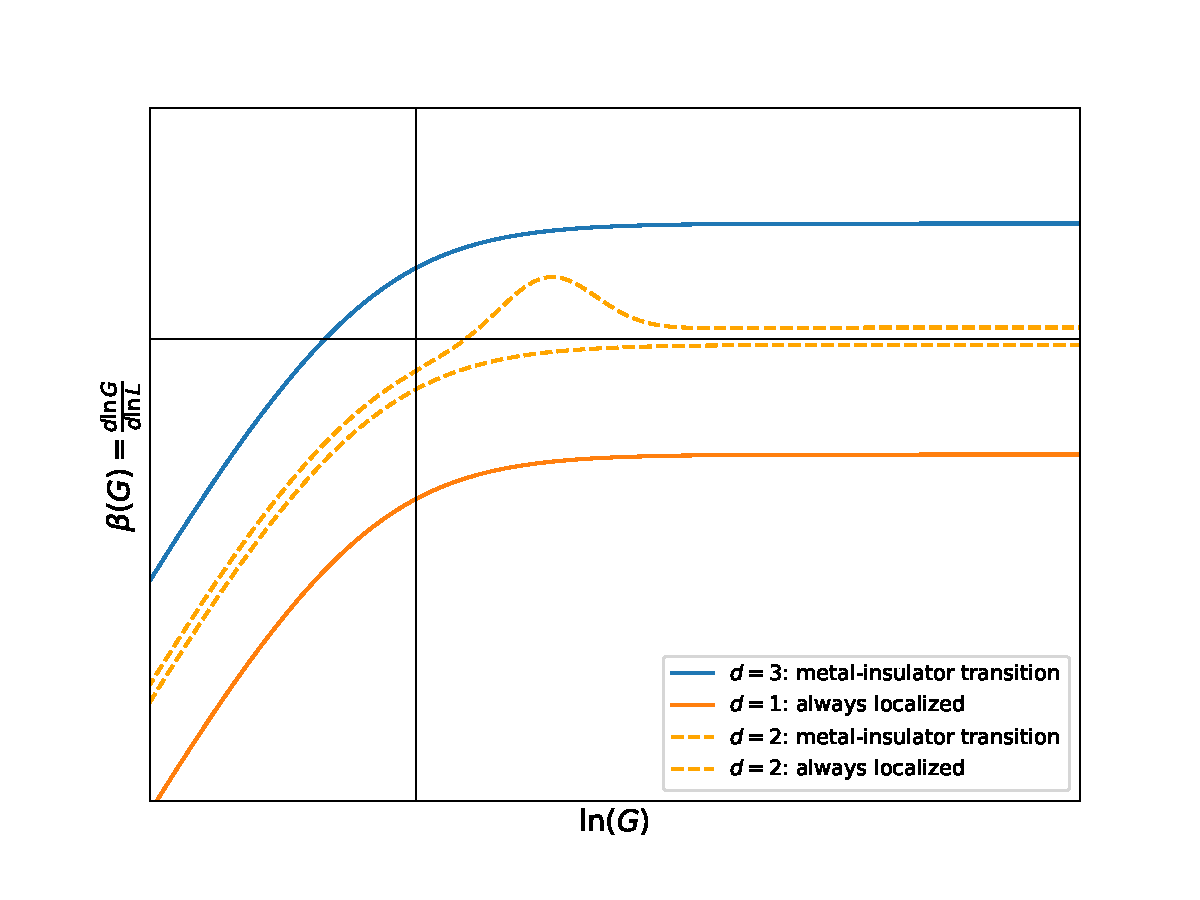
\includegraphics[width=0.7\textwidth]{figures/scaling_of_Anderson_localization.pdf}
              \caption{Schematic Plot on the RG Flow of the Conductance}
              \label{fig:scaling_of_Anderson_localization}
          \end{figure}
\end{itemize}

\section{Complexity from Symmetry and Topology}
Modern classification theory on quantum phases of matter is based on the intrinsic property of the quantum states: quantum entanglement. The concept of \emph{local unitary transformation} (LU) was proposed first in classificaltion of the matrix product states representation of the 1D gapped spin systems
\begin{equation*}
    |\Psi\rangle=\sum_{s_1,\cdots,s_N}\mathop{\mathrm{Tr}}\bigg[A_1^{s_1}A_2^{(s_2)}\cdots A_N^{(s_N)}\bigg]|s_1,s_2,\cdots,s_N\rangle,
\end{equation*}
by Chen, Gu and Wen in \cite{chen2011classification} . They quickly realize that the framework of LU can be generalized to other quantum phases in \cite{chen2010local}, resulting in the famous map:

\subsection{Free fermion Topology: Example of 10-fold Way}
The key feature of SPT state is the presence of the \emph{gapless} edge states that are protected by the symmetry. Namely we


\subsection{Symmetry Enrichment: SPT and SET}
Symmetry protected topological (SPT) order exists in gapped systems with global symmetry. The ground state of the system does not spontaneously break the symmetry, has no fractional excitation, yet cannot be smoothly connected to a product state without explicitly breaking the symmetry. The nontrivial natural of the SPT order can be manifested in two ways:
\begin{enumerate}
    \item As nontrivial edge states which must either be gapless, spontaneously break symmetry or support anomalous SF pattern (with bulk dimension $\geq3$) as long as the global symmetry is not explicitly broken.
    \item For SPT phases with unitary on-site symmetry, gauging the symmetry results in nontrivial gauge theories whose gauge fluxes have nontrivial braiding statistics.
\end{enumerate}

It was shown that a large class of SPT phases in boson/spin systems in dimension d has a one to one correspondence with equivalence classes of group cocycles $H^{d+1}(G, U (1))$ [Witten]. For unitary G, gauging the symmetry results in $d$ dimensional Dijkgraaf-Witten (DW) gauge theory characterized also by the equivalence class of cocycles []. For example, the double semion theory in 2D is a DW gauge theory of gauge group $\mathbb Z_2$ corresponding to the nontrivial element in $H^3 (\mathbb Z_2 , U(1))$. For definition of group cocycles and discussion of their relation with SPTs and gauge theories , see Refs. [].
For the discussion in this review, it suffices to know that the set of equivalence classes of group cocycles in $H^{d+1}(G, U (1))$ forms an abelian group. For $d=0$, elements in $H^1(G, U(1))$ corresponds to one dimensional representations of $G$ which have a one to one correspondence with symmetry charges of $G$. For $d=1$, elements in $H^2(G, U(1))$ corresponds to projective representations of $G$ with $U(1)$ coefficient; such projective representations are realized as degenerate edge states of one dimensional SPT phases. We collect a few simple mathematical results of $H^{d+1}(G, U (1))$, for $d\geq1$, ...


\section{Complexity from Twisting: Moir\'{e} Physics}
\subsection{2D Materials}
\subsubsection{Graphene}
Historically, there exists many arguments claiming the non-existence of 2D materials due to the instability under finite thermal fluctuations\footnote{For example, a naive (so \emph{wrong}) entropy argument goes as following: Note that 2D material has less vibration modes than 3D materials of the same particle number, the entropy contribution from these vibration modes should be smaller in 2D, so is not entropy-favored.}, and even Lev Landau made mistakes here\footnote{Landau claim the non-existence based on the experimental facts that no divergence has been observed under a disorder to order (like liquid to crystal) phase transition.}. All of these arguments are disputed by the discovery of graphene in 2004 by Geim and Novoselov \cite{novoselov2004electric}. And the realistic two-dimensional world has been opened since then.

Graphene is well-known for the appearance of Dirac points in its band structure. For the honeycomb lattice constituted of carbon atoms only, there exists sublattice (inversion) symmetry between $A,B$ sublattices. For spinless electrons, where Hamiltonian is written in such pseudospin basis as a general two-by-two matrix $H(\bm k)=\bm d(\bm k)\cdot\bm \tau$ with real vector coefficients $\bm d(\bm k)$, the inversion operator $\mathcal P$ exchanging $A,B$ sites can be represented as $P=\tau_x$. Graphene also possesses time-reversal symmetry, and for spinless electrons the time-reversal operator is simply a complex conjugate $T=K$. Therefore, the combination of inversion symmetry and time-reversal symmetry keeping the momentum unchanged: $\mathcal P\mathcal T:\bm k\mapsto\bm k$, requires the Hamiltonian to satisfy
\begin{equation*}
    \tau_x^{-1}H^*(\bm k)\tau_x=H(\bm k),
\end{equation*}
implying $d_3(\bm k)=0$ or $H(\bm k)=d_1(\bm k)\tau_x+d_2(\bm k)\tau_y$ with ALL matrix element off-diagonal. Now because both the momentum and the Hamiltonian share the same dimensionality, \emph{given one zero solution of the eigen equation $\det|\lambda I-H(\bm k)|=0$, any perturbation preserving the inversion and time-reversal symmetries, i.e., constituted of $\tau_x$ and $\tau_y$ matrices, cannot destroy such zero point}. That is the typical example of symmetry-protected Dirac points (if exists) in graphene.

To obtain the low-energy description of graphene, we can consider the spatial $C_3$ rotation symmetry at the $K$ and $K'$ points, and implement the constraint from $C_3$ rotation operations that
\begin{equation}\label{eq:C3 rotation constraint}
    C_3^{-1}H(\bm k)C_3=H(\mathcal C_3^{-1}\bm k).
\end{equation}
\noindent Precisely speaking, we can expand the general Hamiltonian around $K$ and $K'$ to the lowest linear-order
\begin{equation*}
    d_1(\bm k)=a_{10}+a_{11}k_x+a_{12}k_y,\quad d_2(\bm k)=a_{20}+a_{21}k_x+a_{22}k_y,\quad d_3(\bm k)=a_{30}+a_{31}k_x+a_{32}k_y,
\end{equation*}
or
\begin{equation*}
    H(\bm k)=\begin{pmatrix}
        a_{30}+a_{31}k_x+a_{32}ky                                & (a_{10}-ia_{20})+(a_{11}-ia_{21})k_x+(a_{12}-ia_{22})k_y \\
        (a_{10}+ia_{20})+(a_{11}+ia_{21})k_x+(a_{12}+ia_{22})k_y & -a_{30}-a_{31}k_x-a_{32}k_y
    \end{pmatrix}
\end{equation*}
and insert back to the constraint Eq. \eqref{eq:C3 rotation constraint}. As a result, one gets
\begin{equation*}
    a_{31}=a_{32}=0,\quad a_{10}=a_{20}=0,\quad a_{12}=-a_{21},\quad a_{11}=a_{22}.
\end{equation*}
Since the diagonal contribution has been excluded from the PT symmetry, we end up with the well-known Dirac cone Hamiltonian
\begin{equation}
    H_K(\bm k)=\hbar v_F\bm k\cdot\bm\tau.
\end{equation}

\subsubsection{Transition Metal Dichalcogenides (TMDs)}
Apart from the typical example of graphene, there are also growing interests in other atomically thin 2D material for their potential application in next-generation of nano devices. In particular, due to its easy fabrication on mechanical exfoliation, transition-metal dichalcogenides (TMD) stands out as the most promising representatives.



TMDs of chemical formula MX$_2$, typically comprise a plane having hexagonally-placed transition metal atoms M (group-IIIB to group-IIB) placed between two chalcogen atom-based hexagonal planes X (e.g., S, Se, Te). There are three monolayer structures: the \emph{trigonal prismatic} 1H phase, the \emph{distorted octahedral} 1T phase, and the \emph{dimerized} 1T' phase, as are shown in Fig. \ref{fig:TMD_electonic_properties}.
\begin{figure}[!htp]
    \centering
    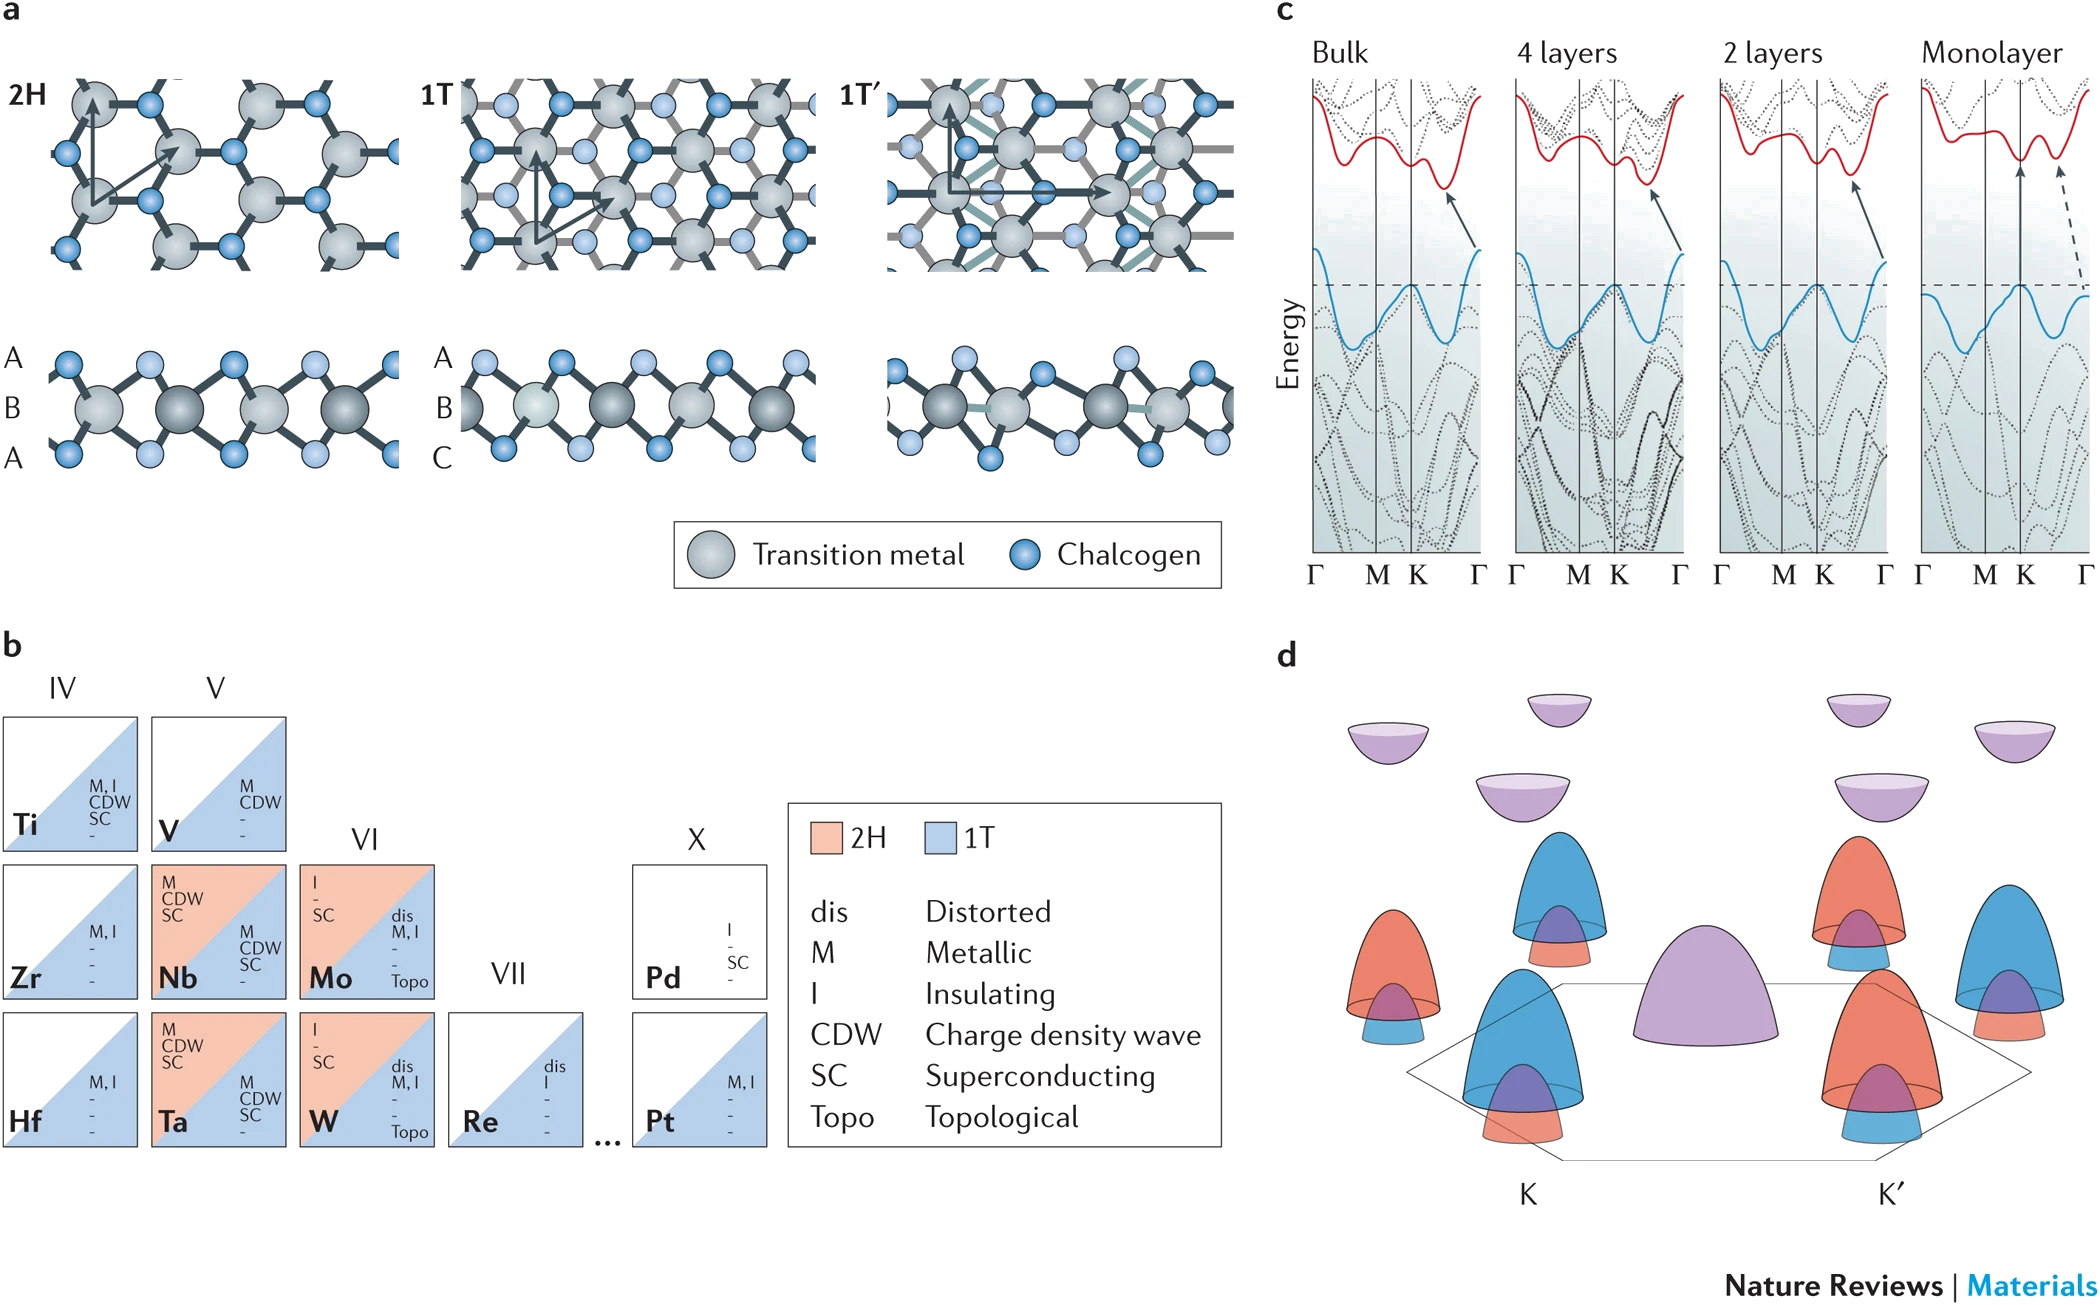
\includegraphics[width=1.0\textwidth]{figures/TMD.png}
    \caption{\textbf{Structure and electronic properties of TMDs} adapted from Ref. \cite{manzeli20172d}. \textbf{a |} Atomic structure of single layers of TMD in their \emph{trigonal prismatic} (2H), \emph{distorted octahedral} (1T) and \emph{dimerized} (1T') phases. \textbf{b |} ``Periodic table'' of known layered TMDs, organized based on the transition metal elements, their existing structural phases (2H, 1T and 1T'), and the observed electronic phases (see the right panel). \textbf{c |} Evolution of the band structure of 2H-MoS$_2$ from bulk material down to monolayers. Clearly a indirect gap to direct gap transition occurs for monolayer material only. \textbf{d |} Schematic band structure of 2H-MoS$_2$, showing the spin splitting (orange and blue colors) at K and K' points.)}
    \label{fig:TMD_electonic_properties}
\end{figure}
We will mostly focus on the group V and group VI transition metal elements, particularly those with 1T and 1T' phases shown to be unstable. So without loss of generalization, when we talk about monolayer TMDs in this thesis, we always refer to the 1H phase structure.
% \begin{figure}[!htp]
%     \centering
%     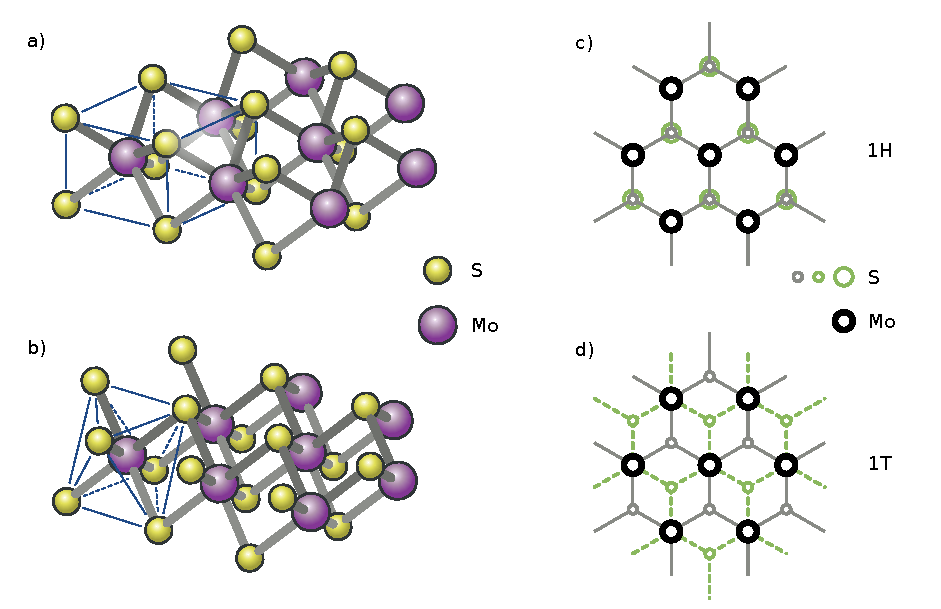
\includegraphics[width=0.8\textwidth]{figures/MoTe2_crystal_structure.pdf}
%     \caption{\textbf{Monolayer $\mathrm{MoS_2}$} (extracted from \url{https://en.wikipedia.org/wiki/Transition_metal_dichalcogenide_monolayers}). a) and c) for 1H phase of monolayer $\mathrm{MoS_2}$, and b) and d) for 1T phase of $\mathrm{MoS_2}$, which is \emph{metastable}. c) and d) are schematic top views, respectively. The 1H ground state has prismatic structure of chalcogen atoms surrounding the transition metal atoms, and the top/bottom layer of chalcogen atoms are the same. The metastable 1T phase shows octahedral structure, less relevant to our discussion, can be viewed by rotating all chalcogen atoms on the top layer by 30 degrees with respect to the lower layers.}
%     \label{fig:MoTe2_crystal_structure}
% \end{figure}
% The 1T phase is \emph{metastable} and is NOT relevant to our discussion. 


For monolayer TMDs of 1H phase, the corresponding bulk material are mostly of 2H stacking form, with alternating alignment of transition metal atoms and chalcogen atoms, as is shown in (a) in Fig. \ref{fig:MoS2_Di}.
\begin{figure}[!htp]
    \centering
    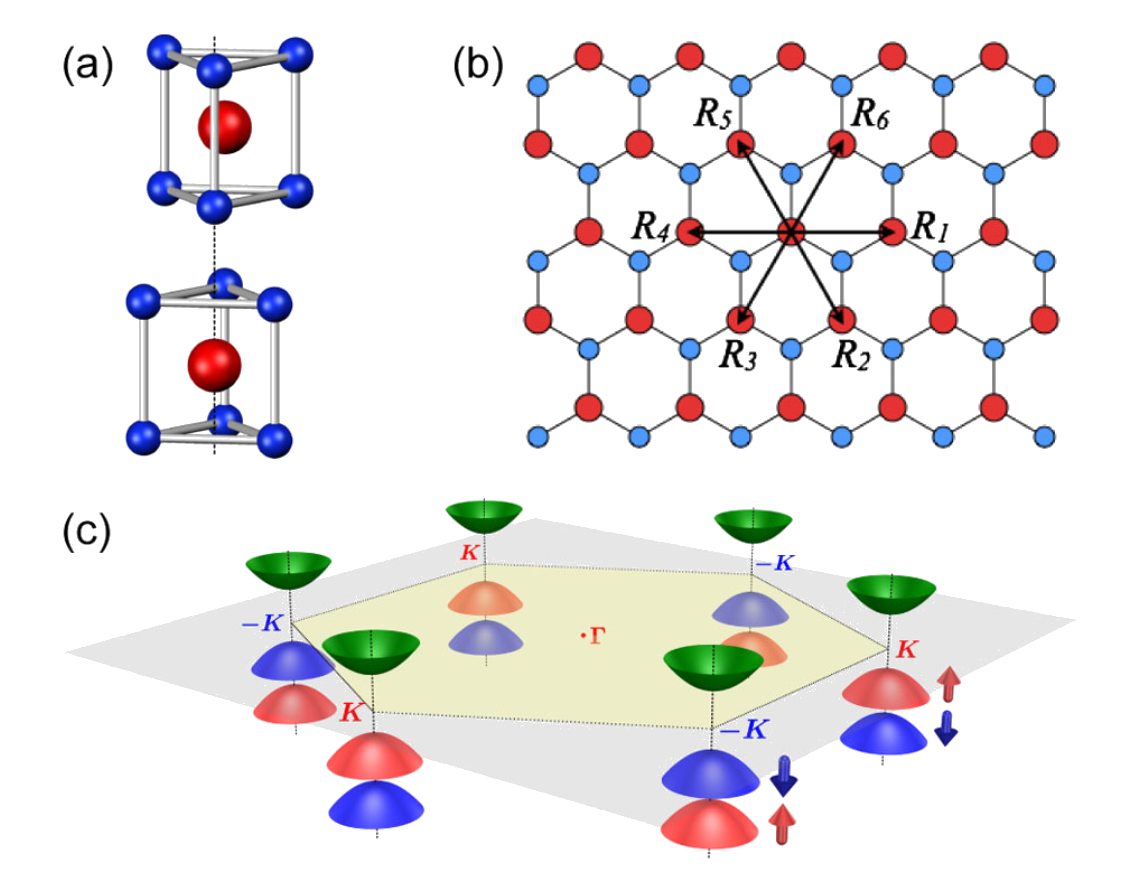
\includegraphics[width=0.8\textwidth]{figures/MoS2_Di.png}
    \caption{Figure adapted from Ref. \cite{xiao2012coupled}. (a) The unit cell of bulk 2H-MoS2. (b) Top view of MoS$_2$ monolayer. (c) Schematic drawing of the band structure at the band edges located at the K points.}
    \label{fig:MoS2_Di}
\end{figure}
Experimentally, there has been reports on the emergence of the peak in the optical spectroscopy study in Ref. \cite{mak2010atomically} and photoluminescence (PL) signals in Ref. \cite{splendiani2010emerging}, which is ascribed as the manifestation on the evolution of of the TMD band structure from bulk's indirect gap to monolayer's direct $K$-$K$ gaps, see (c) in Fig. \ref{fig:TMD_electonic_properties}.

Taking group-IV dichalcogenides MX$_2$ as the example, the 2H stacking bulk material has space group $D_{6h}$ with inversion symmetry (see (a) in Fig. \ref{fig:MoS2_Di}), but reduces to $D_{3h}$ breaking the inversion symmetry down to monolayers. For monolayer MX$_2$, DFT calculation tells that the relevant orbitals within the conduction and valence bands are all from partially-filled d-orbitals \cite{mattheiss1973band}. From symmetry aspect, the trigonal prismatic crystal field splits\footnote{See the character table for point group $D_{3h}$ \url{http://symmetry.jacobs-university.de/cgi-bin/group.cgi?group=603&option=4}.} the d-orbitals of transition metal elements into three groups: $A_1'(d_{z^2})$, $E'(d_{xy}, d_{x^2-y^2})$, and $E''(d_{xz}, d_{yz})$. But the in-plane $z\rightarrow-z$ mirror symmetry forbid the contribution from $E''$ (since both $d_{xz}$ and $d_{yz}$ changes sign under the mirror operation), leaving only $A_1'$ and $E'$ irreps contributing to the band structure.

Now we can start the $\bm k\cdot\bm p$ analysis around $K$ and $K'$ points. Clearly the only possibility to construct the two states orthogonal to each other (corresponding to $K$ and $K'$) is to insert the valley index $\tau=\pm1$ to the below irreps:
\begin{equation*}
    |\phi_1\rangle=|d_{z^2}\rangle, \quad|\phi_{2,\tau}\rangle=\dfrac{1}{\sqrt{2}}(|d_{xy}\rangle+i\tau|d_{x_2-y^2}\rangle)
\end{equation*}
And then the effective Hamiltonian can be expanded in terms of Pauli matrices as $H_\tau(\bm k)=\bm d(\bm k)\cdot\bm\sigma$. The diagonal parts represent the $K$-$K$ (or $K'$-$K'$) direct band gap $\Delta$. Up to the lowest order expansion, we can write
\begin{equation*}
    H=\begin{pmatrix}
        \Delta/2                 & \alpha k_x+\beta k_y \\
        \alpha^* k_x+\beta^* k_y & -\Delta/2
    \end{pmatrix}.
\end{equation*}
Then again due to $C_3$ symmetry, one can show that $\beta=i\alpha$ and we obtain the result
\begin{equation}\label{eq:MoS2 kdotp}
    H=\hbar v_F(\tau k_x\sigma_x+k_y\sigma_y)+\frac{\Delta}{2}\sigma_z.
\end{equation}

Now let us include the spin-orbit couplings (SOC) $\lambda\bm L\cdot\bm S$. This is equivalent to evaluate the matrix element $\langle \phi_{\alpha, s_1}|\bm L\cdot\bm S|\phi_{\beta, s_2}\rangle$.

\begin{equation}
    H_{\text{SOC}}=\lambda\bm\sigma\cdot(\nabla U\times\bm p)
\end{equation}

Standard $\bm k\cdot\bm p$ theory tells that the SOC contribution is to evaluate the

% \ref{fig:monolayer_TMD_band_structure}.
% \begin{figure}[!htp]
%     \centering
%     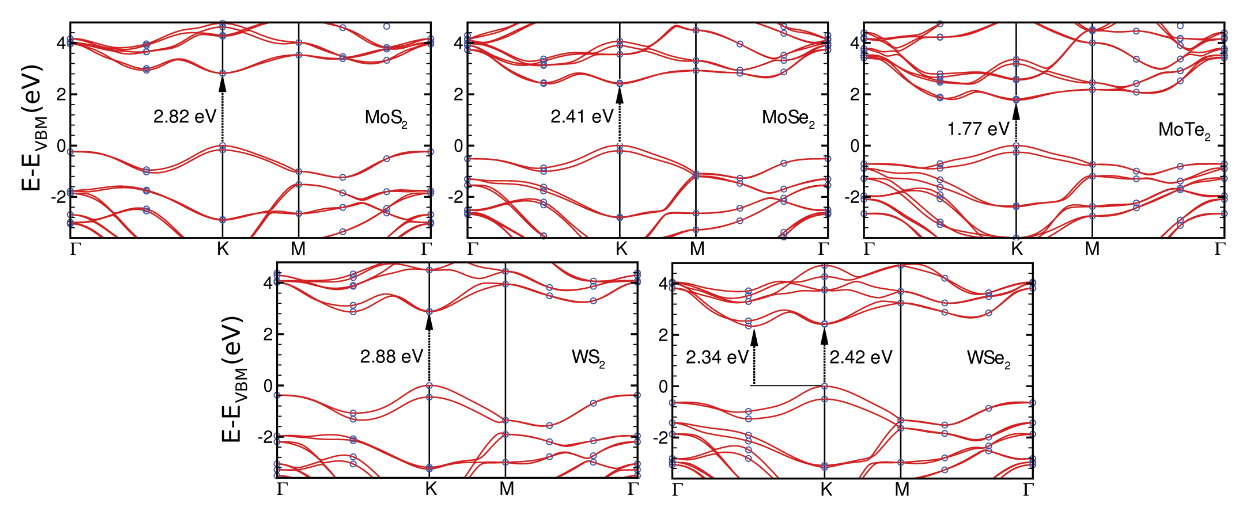
\includegraphics[width=0.8\textwidth]{figures/monolayer_TMD_band_structure.png}
%     \caption{DFT band structures for several MX$_2$ monolayer materials (extracted from \cite{ramasubramaniam2012large}).}
%     \label{fig:monolayer_TMD_band_structure}
% \end{figure}

% For typical monolayer TMD material, there are gap

% The M-X bonds within layers are mostly covalent, while weak Van der Waals forces hold the sandwiched layers. A

% Taking the prototypical group-VI dichalcogenide as the example, for example $\mathrm{MoS_2}$, a nice feature of



\subsection{Twisting with Moir\'{e} Physics}
Moir\'e patterns are known as the interference patterns generated when two or more periodic structures are overlaid. The interference pattern exhibits a new large-scale periodic structure (coin as \emph{Moir\'{e} scale}) on top of the original one, so that the original lattice information is smeared out, leaving physics occurring at such new Moir\'{e} scale $a_M\sim a/\theta$. In momentum-space, this is equivalent to have a largely reduced Moir\'e Brillouin zone (mBZ) with the Moir\'e reciprocal vector $b_M\sim \theta b$, \textbf{giving rise to a large number of $N_M\sim N/\theta^2$ Moir\'e bands due to the \emph{zone folding effect}}. This is desirable since the new Moir\'e unit cell now encloses a number of $N_M\sim N/\theta^2$ atoms from the $N$ atoms within the orignal unit cell. Clearly not all value of $\theta$ gives an integer $N_M$. Those $\theta$ that indeed gives an integer $N_M$ are \emph{commensurate} angles. However, in the small twisting regime where $N_M\gg1$, it is OK to always take $N_M$ as an integer, and consider \emph{incommensurate angles} as well.

As a result, the band width $\Delta$ of the original periodic structure is also highly suppressed to $\Delta\theta^2$ within mBZ. Plus the possible tunnelings between different mBZ sectors, which has no reason to stay to be zero, we will naturally end up with gapped Moir\'e bands as isolated \emph{flat bands}, where strong correlations play important roles because the electron kinetics are almost quenched. To sum up, the Moir\'e Hamiltonian can be constructed as the following two steps:
\begin{enumerate}
    \item Enlarge unit cell to Moir\'e super unit cell, which is equivalent to partition the original BZ into many mBZ connected with Moir\'e reciprocal vectors. This serve as the diagonal part of the huge Moir\'e Hamiltonian.
    \item These mBZs can talk to each other through the interlayer tunnelings. This will serve as the off-diagonal part of the Moir\'e Hamiltonian.
\end{enumerate}

\subsubsection{Twisted Bilayer Graphene}
Before dive into the details, let us first fix the geometry of twisted bilayer graphene (tBLG). For each layer, we take the bravias vector $\bm a_1=\frac{a}{2}(\sqrt{3},3), \bm a_2=\frac{a}{2}(-\sqrt{3},3)$ with the sublattice crystal vector $\bm\delta_A=\bm 0, \bm\delta_B=\frac{1}{3}(\bm a_1+\bm a_2)$, so that the reciprocal vector reads $\bm b_1=\frac{2\pi}{3a}(\sqrt{3},1), \bm b_2=\frac{2\pi}{3a}(-\sqrt{3},1)$, and the BZ edge $K$-point is $\bm K=\frac{1}{3}(\bm b_1-\bm b_2)$. Monolayer graphene is known for the presence of Dirac points at $K$ (or $K'$) points. Denoting the layer index as $l=\pm1$, we can start with stacking two Dirac cone Hamiltonian around $K$ (or $K'$) point with separated top/bottom bloch basis ${|\bm k_l,\alpha\rangle}$
\begin{equation*}
    H_K = \sum_{l=\pm 1}\sum_{\bm k_l\in\text{BZ}_l}\sum_{\alpha\alpha'} c_{\bm k_l,\alpha'}^\dagger \hbar v_F[(\bm k_l-\bm K_l)\cdot\bm\sigma]_{\alpha'\alpha} c_{\bm k_l,\alpha}.
\end{equation*}

As is discussed above, if we stack two layers of graphene with a relative commensurate twist angle $\theta$. The Moir\'e Hamiltonian should be constructed by partitioning the sum of orignal Bloch states $|\bm k\rangle$ for $\bm k\in\text{BZ}$ into the sum within the mBZ, plus the sum over distinct mBZ sectors connected with Moir\'e reciprocal vectors
\begin{equation*}
    \{|\bm k_l\rangle\}_{\bm k_l\in\text{BZ}}\rightarrow\{|\bm k_l+\bm Q_l\rangle\}_{\bm k_l\in\text{mBZ},\bm Q_l=\{l_1\bm b_{M1}+l_2\bm b_{M2}\}}.
\end{equation*}

As is seen in Fig. \ref{fig:tBLG_geometry}.

\begin{figure}[!htp]
    \centering
    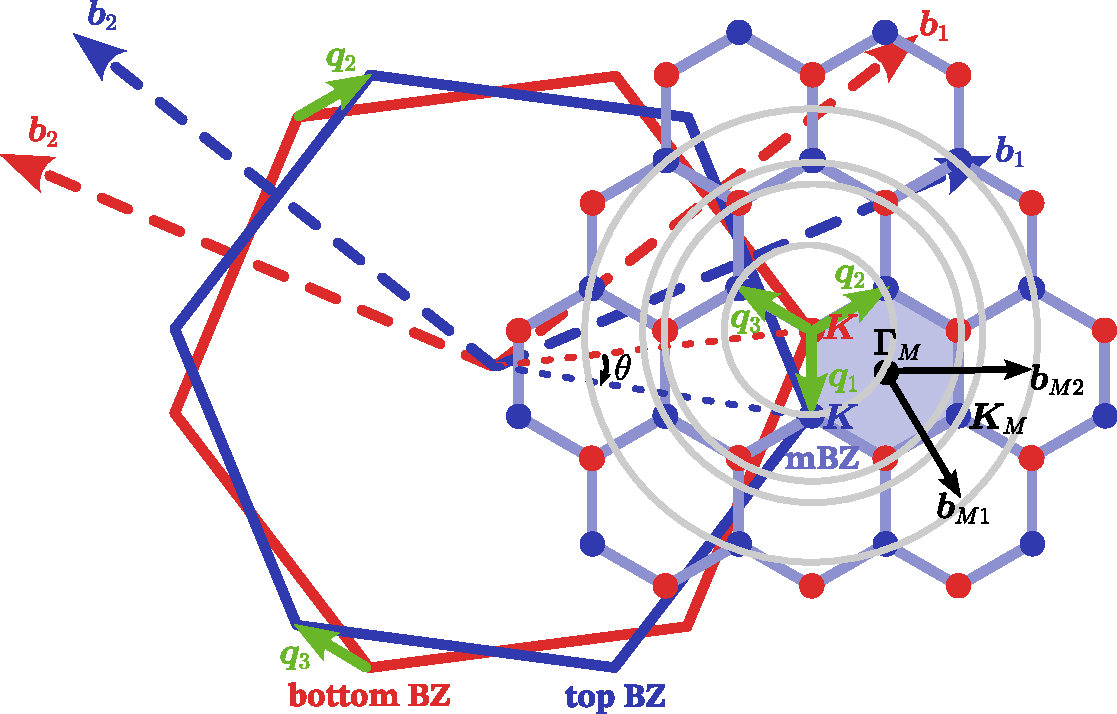
\includegraphics[width=0.95\textwidth]{figures/tBLG_geometry.pdf}
    \caption{Moir\'e Brillouin Zone of Twisted Bilayer Graphene. Blue (top) hexagonal BZ is rotated by $-\theta/2$, red (bottom) hexagonal BZ is rotated by $\theta/2$. The Moir\'e BZ (mBZ) is the shaded hexagonal. Gray dashed circles represents the truncation shells for the interference of interlayer tunnelings.}
    \label{fig:tBLG_geometry}
\end{figure}

Next step is to consider the tunnelings among each mBZ sectors. Generally, this is to think about the interlayer tunneling matrix elements for some interlayer tunneling Hamiltonian $H_{\text{interlayer}}$:
\begin{align*}
    T_{\bm k_l,\alpha;\bm k_{l'},\alpha'} & = \langle\bm k_l,\alpha|H_{\text{interlayer}}|\bm k_{l'},\alpha'\rangle                                                                                                                                                                 \\
                                          & \equiv\frac{1}{N}\sum_{\bm R_l,\bm R_l'}\sum_{\alpha,\alpha'} e^{-i\bm k_l\cdot(\bm R_l+\bm\delta_{l,\alpha})}e^{i\bm k_{l'}\cdot(\bm R_{l'}+\bm\delta_{l',\alpha'})}t(\bm R_l+\bm\delta_{l,\alpha}, \bm R_{l'}+\bm\delta_{l',\alpha'})
\end{align*}
where we recognize the real-space tunneling between Wannier centers $\langle\bm R_l,\alpha|H_{\text{interlayer}}|\bm R_l',\alpha'\rangle\equiv T(\bm R_l+\bm\delta_{l,\alpha}, \bm R_{l'}+\bm\delta_{l',\alpha'})$. And because Wannier center is highly localized, \emph{two-center approximation} \cite{bistritzer2011moire} can be made so that $T(\bm R_l+\bm\delta_{l,\alpha}, \bm R_{l'}+\bm\delta_{l',\alpha'})\simeq T(\bm R_l+\bm\delta_{l,\alpha} - \bm R_{l'}-\bm\delta_{l',\alpha'})$. Introducing the Fourier component of the the real-space tunneling $t_{ll'}^{\alpha\alpha'}(\bm q)$ (due to translation symmetry)
\begin{align*}
    T(\bm R_l+\bm\delta_{l,\alpha} - \bm R_{l'}-\bm\delta_{l',\alpha'}) & = \frac{1}{N}\frac{1}{A}\sum_{\bm q}t_{ll'}^{\alpha\alpha'}(\bm q) e^{i\bm q\cdot(\bm R_l+\bm\delta_{l,\alpha} - \bm R_{l'}-\bm\delta_{l',\alpha'})},
\end{align*}
we have
\begin{align}
    T_{\bm k_l,\alpha;\bm k_{l'},\alpha'} & =\frac{1}{A}\sum_{\bm q}\left(\frac{1}{N}\sum_{\bm R}e^{i\bm R_l\cdot(\bm q-\bm k_l)}\right)\left(\frac{1}{N}\sum_{\bm R'}e^{-i\bm R_{l'}\cdot(\bm q-\bm k_{l'})}\right) \sum_{\alpha\alpha'} t_{ll'}^{\alpha\alpha'}(\bm q) e^{i\bm \delta_{l,\alpha}\cdot\bm(\bm q-\bm k_l)}e^{-i\bm\delta_{l',\alpha'}\cdot(\bm q-\bm k_{l'})} \nonumber \\
                                          & = \frac{1}{A}\sum_{\bm q}\sum_{\bm G_l}\delta_{\bm q-\bm k_l,\bm G_l}\sum_{\bm G_{l'}}\delta_{\bm q-\bm k_{l'},\bm G_{l'}}\sum_{\alpha\alpha'} t_{ll'}^{\alpha\alpha'}(\bm q) e^{i\bm \delta_{l,\alpha}\cdot\bm(\bm q-\bm k_l)}e^{-i\bm\delta_{l',\alpha'}\cdot(\bm q-\bm k_{l'})}                                                \nonumber \\
                                          & = \sum_{\bm G_l,\bm G_{l'}}\sum_{\alpha\alpha'} \frac{t_{ll'}^{\alpha\alpha'}(\bm k_l+\bm G_l)}{A} e^{i\bm\delta_{l,\alpha}\cdot\bm G_l}e^{-i\bm \delta_{l',\alpha'}\cdot\bm G_{l'}}\delta_{\bm k_l+\bm G_l,\bm k_{l'}+\bm G_{l'}}.\label{eq:two-center_approximation}
\end{align}
The momentum-space expression Eq. \eqref{eq:two-center_approximation} is the general result of the two-center approximation. The Dirac delta function signatures the momentum convervation of the tunneling processes.

In the setup of twisted bilayer graphene, Eq. \eqref{eq:two-center_approximation} can be further simplified by looking at the small shift around the $K$ or $K'$ point $\bm k_l\rightarrow\bm k_l+\bm K_l$ for $|\bm k_l|\ll1$.



\subsubsection{Twisted TMD}
For bilayer Moir\'e materials, the Moir\'e interference patterns can be formed when two layers (not have be fully identical) are relatively displaced with a vector $\bm d$ and properly rotated by some \emph{commensurate} angle $\theta$.


It has been already shown in monolayer group-IV TMDs that the strong spin-orbit coupling and broken inversion symmetry lifts spin degeneracy within the conduction band $\sim100$meV. Thus for a bilayer TMD material of the same kinds (\emph{homobilayer}), for example, twisted bilayer MoTe$_2$, the $K$ or $K'$ valley valence band (pinned with spin) can be separated out in our discussion, resulting a simple two-band model with layer pseudospin at each valley.



\subsection{Twisting without Moir\'{e} Physics}
\subsubsection{Twisted Cuprates}

% \chapter{Supercurrent-induced Anomalous Thermal Hall Effect as a New Probe to Superconducting Gap Anisotropy}

\begin{abstract}
    Two-dimensional superconductors have been realized in various atomically thin films such as the twisted bilayer graphene, some of which are anticipated to involve unconventional pairing mechanism. Due to their low dimensionality, experimental probes of the exact nature of superconductivity in these systems have been limited. We propose, by applying a \emph{vertical} supercurrent to a bilayer superconductor where the mirror symmetry is naturally broken by the twisting, there will be anomalous thermal Hall effect induced by the supercurrent that can serve as a sharp probe for the \emph{in-plane} anisotropy of the superconducting gap function. This effect occurs in the \emph{absence} of an external magnetic field and spontaneous breaking of the time-reversal symmetry in the ground state. We derive explicit formulas for the induced thermal Hall conductivity and show them to be significant in the examples of twisted cuprates and twisted FeSe where monolayer superconductivity have already been observed. Though technical challenges still exist, we propose this to be a generic probe of the gap anisotropy in a twisted bilayer superconductor.
\end{abstract}

\section{Introduction}
The discovery of the correlated insulating phases and superconductivity in twisted bilayer graphene (TBG) \cite{cao2018unconventional,cao2018correlated} has spurred intense interest in twisted two-dimensional (2D) heterostructures, leading to the notion of \emph{twistronics} as a new form of electronic device. To understand the (possibly unconventional) superconductivity realized in these systems, intense experimental investigations have been on-going \cite{oh2021evidence,kim2022evidence,lake2022pairing}. While the majority of transport studies on twisted bilayers focuses on electrical transport at the moment, thermal transport has long been established as a powerful and complementary tool for investigating the nature of elementary excitations, particularly in superconductors where ordinary electric transport measurement is ineffective \cite{krishana1997plateaus,chiao2000low,sutherland2003thermal,durst2003weak,zhang2001giant,cvetkovic2015berry}. More recently, quantized thermal Hall conductivity at low temperature became a signature of the topologically ordered ground states in correlated materials \cite{banerjee2018observation,yokoi2021half}. In this work, we show that the thermal Hall response can be a sensitive probe of the {\it gap anisotropy} in twisted bilayer superconductors, or TBS for short. 

The gap function $\varDelta_{\bm{k}}$ of a superconductor has immense implications for the underlying pairing mechanism and the quasiparticle transport. It may be deduced in the angle-resolved photoemission spectroscopy (ARPES) \cite{shen1993anomalously,ding1996angle,zhang2016superconducting}, or through the quasiparticle interference (QPI) imaging in scanning tunneling spectroscopy \cite{hanaguri2007quasiparticle,sprau2017discovery}. Resolving the gap anisotropy in ARPES becomes challenging though for low temperature superconductors where $\varDelta_{\bm{k}}$ is smaller than the experimental resolution. For twisted heterostructures, resolving the momentum space structure within a small moir\'e Brillouin zone (BZ) necessitates the QPI imaging over a formidably large area in the real space. As the demand to resolve the gap structure in TBS grows, limitations of existing experimental probes seem to loom larger. A natural question to ask, at this stage, is whether it is possible to invent a new probe of the gap anisotropy for very small $\varDelta_{\bm{k}}$. Here we propose a supercurrent-induced anomalous thermal Hall effect (SATHE) as one possible way to directly probe the gap anisotropy in TBS. 

Fig \ref{fig: setup}.(a) shows the schematic setup for SATHE. The TBS may be a vertical Josephson junction (JJ) formed by stacking two atomically thin superconducting films with a certain twist angle, or an intrinsic twisted bilayer superconductor as in TBG. SATHE is a nonlinear response of heat, created by simultaneously applying a \emph{vertical} supercurrent $\bm J_S$ and an {\it in-plane} temperature gradient, with the resulting {\it transverse in-plane} flow of heat. In contrast to the conventional thermal Hall effect (THE) which occurs when the ground state breaks the time-reversal symmetry (TRS), SATHE can occur for ground states that preserve the TRS. No external magnetic field is required to observe SATHE. 

\begin{figure}[!ht]
	\centering
	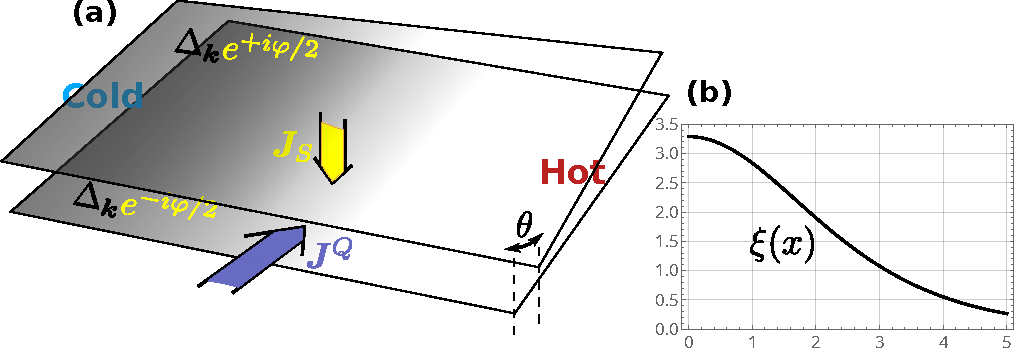
\includegraphics[width=0.8\textwidth]{contents/SATHE/figures/illustration.pdf}
	\caption{(a) SATHE for bilayer-SC. The vertical supercurrent $\bm{J}_S$, or equivalently, a pairing phase twist $\varphi$ between the two layers of, either a vertical JJ or an intrinsic bilayer superconductor, would induce an in-plane thermal Hall effect in a bilayer superconductor. In the former case, an insulating buffer layer may be present (not shown).  (b) an illustration for the dimensionless function $\xi(x)$ in Eq.(\ref{eq:xi}).}
	\label{fig: setup}
\end{figure}

Our proposal thus differs for most proposals of THE including, for instance, Ref. \cite{can2021high} where the JJ spontaneously breaks TRS in the absence of applied supercurrent. It bear resemblance to the Sodemann-Fu proposal for nonlinear electrical Hall effect \cite{sodemann2015quantum,ma2019observation}, in that in both proposals the \emph{unperturbed} ground state preserves TRS. One can think of the nonlinear electrical Hall effect as arising from the first electric field driving an imbalance of the fermion distribution, and the second electric field is used to probe the Hall response. In our proposal, the supercurrent is employed to drive Berry curvature out of its equilibrium form, then a temperature gradient is applied to induce the thermal Hall response. In this sense, SATHE can be taken as a thermal analogue of the nonlinear Hall effect.

When the supercurrent is not too large, one can linearize the current-phase relation $\bm J_S \propto\varphi$ and SAHTE becomes the perturbative change of the thermal Hall conductivity $\delta \kappa_{xy}$ proportional to the phase twist, $\delta\kappa_{xy}\simeq\varphi\cdot\chi_{\varphi xy}$, with $\chi_{\varphi xy}$ capturing the nonlinear response of the system. Similar to nonlinear Hall effect, the breaking of inversion symmetry is necessary to elicit the desired responses. The observation of SATHE additionally requires the breaking of in-plane and out-of-plane mirror symmetries, which are not conditions normally present in the family of nonlinear Hall effects, but are naturally satisfied in the TBS. The conditions for observing SATHE are therefore not any more stringent than those of other proposed nonlinear Hall effect, at least from the perspective of symmetry requirement. 

\section{Main Results}
For TBS with a multiband electronic structure, the pairing Hamiltonian is generally $\sum_{a,b} \varDelta_{\bm{k}}^{a,b} c^\dagger_{a,\bm{k}} c^\dagger_{b,-\bm{k}}$, with $a,b$ ranging over the bands. We firstly study the simple situation where only the \emph{intraband pairing} is present: $\varDelta_{\bm{k}}^{a,b}=0$ for $a\neq b$. Assuming that $|\varDelta_{\bm{k}}|$ is much smaller than the energy difference between bands in the normal state,  we find that a small pairing phase difference $\varphi$ between the layers in the TBS induces a change of the Berry curvature and leads to the SATHE formula
\begin{align}
    & \frac{\delta\kappa_{xy}^{\text{intra.}}}{T} = \varphi\cdot \frac{\chi_{\varphi xy}^{\text{intra.}}}{T} =\varphi \cdot\frac{k_B^2}{16\pi^2\hbar} \sum_{\text{FS}}\mathop{\mathrm{sign}}(v_F)\notag\\
	% \frac{\delta\kappa^{\text{intra.}}_{xy}}{\delta\varphi\cdot T}=&\frac{k_B^2}{16\pi^2\hbar} \sum_{\text{FS}}\mathop{\mathrm{sign}}(v_F)\notag\\
	&\qquad\times\oint_{\text{FS}}\dd k_\parallel\,\xi\bigg(\frac{\varDelta_{\bm{k}}(T)}{k_BT}\bigg)\cdot\partial_{k_\parallel} [\langle u_{\bm{k}}|\hat L|u_{\bm{k}}\rangle] .  \label{eq:main_result}
\end{align}
Here $\chi_{\varphi xy}^{\text{intra.}}$ is the intraband transport coefficient for SATHE, $\xi(x)$ is the dimensionless function (see Fig.\ref{fig: setup} (b))
\begin{align}\label{eq:xi}
	\xi(x)\equiv\int_{|x|}^\infty\mathrm{d}x' \sqrt{x'^2-x^2}\frac{x'}{1+\cosh(x')},
\end{align}
and $|u_{\bm{k}}\rangle$ is the Bloch state at the Fermi level in the \emph{normal} state. The dimensionless Hermitian operator $\hat L$ is the generator of Doppler shift due to $\varphi$, and equals $\hat L=\mathop{\mathrm{diag}}\{\mathbf{1},\mathbf{-1}\}$ in the layer space  for a vertical JJ but gets more complicated for an intrinsic bilayer superconductor (see below and Supplemental Material (SM) \cite{SM}). The loop integral is performed over each Fermi surface (FS) and $k_\parallel$ is the counterclockwise tangential momentum at the Fermi surface. The $\mathop{\mathrm{sign}}(v_F)=\pm 1$ characterizes whether the FS is electron-like or hole-like (a single band may host multiple FS's). Clearly if $\varDelta_{\bm{k}}$ is $\bm{k}$-independent, the loop integral over the FS reduces to a total derivative and vanishes identically.

\section{The $\hat L$ operator and Doppler shift}
The normal state tight-binding Hamiltonian for the bilayer can be written in a block form:
\begin{align}
	H_0(\bm{k})=\begin{pmatrix} H_0^t(\bm{k}) & T_\perp(\bm{k}) \\ T^\dagger_{\perp}(\bm{k}) & H_0^b(\bm{k})\end{pmatrix},\label{eq:H_0}
\end{align}
where $t/b$ labels the top/bottom layer, and $T_\perp$ represents the interlayer hopping. In the superconducting state, pairing terms are introduced. Introducing the pairing phase difference $\varphi$ due to the applied supercurrent is equivalent to performing a gauge transformation $H_0\rightarrow U (\varphi) H_0U^\dagger (\varphi)$ (Doppler shift) while keeping the pairing terms unchanged, and $\hat L$ is its generator: $U(\varphi)\equiv e^{-i\frac{\varphi}{4} \hat L}$. For a vertical JJ, $\hat L=\mathop{\mathrm{diag}}\{\mathbf{1},\mathbf{-1}\}$. For an intrinsic superconductor, $\hat L$ depends on the atomic orbital positions normal to the bilayer plane (see SM \cite{SM} and also Ref. \cite{crowley2022supercurrent} therein).

For a JJ, since $|u_{\bm{k}}\rangle$ is the eigenstate of $H_0(\bm{k})$, $\langle u_{\bm{k}}|\hat L|u_{\bm{k}}\rangle \in [1,-1]$ serve as the indicator of the layer-component of the state. If $T_\perp$ is absent, top/bottom layers decouple and $\langle u_{\bm{k}}|\hat L|u_{\bm{k}}\rangle =\pm 1$, leading to vanishing SATHE according to Eq.(\ref{eq:main_result}), consistent with physical intuitions. 

\section{Derivation of Eq. (\ref{eq:main_result})}
Here we show how to derive the SATHE formula of Eq. (\ref{eq:main_result}) while leaving the more technical parts to \cite{SM}. The thermal Hall conductance in a 2D superconductor is  related to the superconducting Berry curvature \cite{qin2011energy,sumiyoshi2013quantum} as
\begin{align}
	\frac{\kappa_{xy}}{T}=-\frac{k_B^2}{2\hbar}\int_{-\infty}^\infty dE \frac{E^2}{(k_B T)^2} \boldsymbol{\sigma}(E) f'(E),\label{eq:kappa}
\end{align}
where $f(E)$ is the Fermi-Dirac function, and 
\begin{align}
	\boldsymbol{\sigma}(E)\equiv -\sum_\mathbf{a} \int_{E_{\bm{k}}<E} \frac{d^2k}{(2\pi)^2} \boldsymbol{\Omega}^\mathbf{a}_{\bm{k}}. \label{eq:sigma}
\end{align}
(Bold fonts are used for quantities related to the superconducting BdG state, to be distinguished from the normal state ones.) Here $\boldsymbol{\Omega}^\mathbf{a}_{\bm{k}}=-2\mathop{\mathrm{Im}}\langle\partial_{k_x} \mathbf{u}^\mathbf{a}_{\bm{k}}|\partial_{k_y} \mathbf{u}^\mathbf{a}_{\bm{k}}\rangle$ is the superconducting Berry curvature while $\mathbf{a}$ labels bands of the Bogoliubov–de Gennes (BdG) Hamiltonian
\begin{align}\label{eq:H}
\mathbf H(\bm{k})=\left(\begin{array}{cc}
		H_0(\bm{k}) & \boldsymbol{\Delta}_{\bm k} \\
		\boldsymbol{\Delta}_{\bm k} & -H_0(\bm{k})
	\end{array}\right).
\end{align}
The BdG Hamiltonian \eqref{eq:H} is written in the Nambu basis $\{\psi_{ \bm k},\Lambda^\dagger\psi_{-\bm k}^\dagger\}$ where $\psi_{\bm k}$ is a collection of fermion operators in the band basis, and $\boldsymbol{\Delta}_{\bm k}^\dagger=\boldsymbol{\Delta}_{\bm k}$. The time reversal transformation works on $\psi_{\bm k}$ as $\psi_ {\bm k}\rightarrow \Lambda K \psi_{\bm k}$, where $K$ is complex conjugation and $\Lambda$ is some unitary operation.  

The energy eigenvalues of the BdG Hamiltonian are ordered into pairs $\pm \mathbf E_{1,\bm{k}},\pm \mathbf E_{2,\bm{k}},\cdots$ with $\mathbf E_{1,\bm k}<\mathbf E_{2,\bm k}<\cdots$ and $\mathbf a=\pm1,\pm2,\cdots$ are used to label the bands such that $\mathbf E_{-\mathbf a,\bm{k}}=-\mathbf E_{\mathbf a,\bm{k}}$. Assuming only the intraband pairing is present, we have $\mathbf E_{|\mathbf a|,\bm{k}}=(\epsilon_{|\mathbf a|,\bm{k}}^2+\varDelta_{|\mathbf a|,\bm{k}}^2)^{1/2}$, where $\epsilon_{a,\bm{k}}$ is the normal state band energy ($a=1,2,...$). We assume that only the $a=1$ band crosses the Fermi level, and all other bands lie strictly above or below it. This allows us to define the interband energy scale as $t\equiv \min |\epsilon_{b,\bm{k}}|$ ($b\neq 1$). The gap function of the first band is defined as $\varDelta_{\bm{k}}\equiv \varDelta_{1,\bm{k}}$. We will consider the weak-pairing limit $|\varDelta_{\bm{k}}|\ll t$, so only the lowest-energy states with $\mathbf a=\pm 1$ need to be included to the leading-order $\varDelta_{\bm k}/t$ expansion of the Berry curvature
\begin{align}
	\boldsymbol \Omega ^{\mathbf a}_{\bm{k}}  \doteq -\mathop{\mathrm{Im}}\left\{\frac{\mathop{\mathrm{Tr}}[\mathbf P_{\mathbf a} \partial_{k_x} \mathbf H \mathbf P_{-\mathbf a} \partial_{k_y}\mathbf H \mathbf P_{\mathbf a}]}{(\mathbf E_{\mathbf a}-\mathbf E_{-\mathbf a})^2}-(x\leftrightarrow y)\right\},\label{eq:Omega}
\end{align}
where $\mathbf P_{\mathbf a}\equiv |\mathbf u^{\mathbf a}_{\bm{k}}\rangle\langle {\mathbf u}^{\mathbf a}_{\bm{k}}|$ is the projector in the Nambu space.

After a small phase twist $\varphi$ is turned on, $\mathbf H, \mathbf E_{\pm\mathbf a}, \mathbf P_{\pm \mathbf a}$ appearing in Eq. (\ref{eq:Omega}) all receive some corrections, which propagate through the THE formulas in Eqs. \eqref{eq:kappa} and \eqref{eq:sigma}. However, as shown in \cite{SM}, only the change in $\mathbf P_{\pm \mathbf a}$ is important when the unperturbed ground state obeys TRS. In the end, the intraband pairing contribution gives 
\begin{align}
	\delta \boldsymbol\Omega^{\mathbf a,\text{intra.}}_{\bm{k}}&\doteq \varphi\sum_{\mathbf b\neq \pm\mathbf a}4 \mbox{Im\,Tr}[ ( \partial_{k_x}\mathbf P_{\mathbf a} ) ( \partial_{k_y}\mathbf P_{-\mathbf a} ) \mathbf P_{\mathbf b} (\partial_\varphi\mathbf P_{\mathbf a} ) \mathbf P_{\mathbf a}]\notag\\
    &\qquad-(x\leftrightarrow y),
\end{align}
To the leading order of $\varDelta_{\bm k}/t$ expansion and focusing on the $\mathbf a = \mathbf 1$ band, we find
\begin{equation}
	\delta \boldsymbol\Omega^{\mathbf 1,\text{intra.}}_{\bm{k}}=-\varphi\cdot\frac{\varDelta_{\bm{k}}^2}{4\mathbf E_{\mathbf 1}^3}\big(v_x \partial_{k_y} - v_y \partial_{k_x}\big)\langle u^1_{\bm{k}}|\hat L|u^1_{\bm{k}}\rangle,\label{eq:Omega_intra}
\end{equation}
with $v_{x,y}\equiv \partial_{k_{x,y}} \epsilon_{1,\bm{k}}$ the normal state Fermi velocity. 

The change in Berry curvature is now fully described with normal state wave functions, and exhibits high concentration near the Fermi surface due to  $\mathbf{E}_{\mathbf 1}^3$ in the denominator. Identifying $\hat L|u_{\bm k}^1\rangle=4i\partial_\varphi|u_{\bm k}^1\rangle$, the derivative $\partial_{k_y}\langle u_{\bm k}^1|\hat L|u_{\bm k}^1\rangle=4\Omega_{y,\varphi}$ becomes the \emph{$\varphi$-twist Berry curvature}, with one component along the momentum direction and the other along the phase twist $\varphi$.

Equation \eqref{eq:Omega_intra} thus demonstrates how the change of Berry curvature in the superconducting state is intricately composed of the gap function, and a mixed Berry curvature in the momentum-phase space. Plugging Eq. (\ref{eq:Omega_intra}) into Eq. (\ref{eq:kappa}) and after some efforts, the main result of our paper Eq. (\ref{eq:main_result}) is established. 


\section{Interband pairing and nodal superconductivity}
When interband pairing is present, the calculation becomes more sophisticated but the final result turns out to be simple. Introducing the normal state projector $P_c\equiv |u^c_{\bm{k}}\rangle\langle u^c_{\bm{k}}|$, the interband pairing gives $\boldsymbol\Delta_{\bm{k}}^{\text{inter.}}=\sum_{b\neq c}P_b \boldsymbol\Delta_{\bm{k}} P_c$, which can be eliminated from the BdG Hamiltonian in Eq. (\ref{eq:H}) by a small unitary rotation 
\begin{equation}
    e^{i\mathcal S\otimes\bm\tau_2}\mathbf H(\bm k) e^{-i\mathcal S\otimes\bm\tau_2}\doteq H_0(\bm k)\otimes\bm\tau_3 + \boldsymbol\Delta_{\bm k}^{\text{intra.}}\otimes\bm\tau_1 .
\end{equation}
Here $\bm\tau$ are Pauli matrices in the Nambu space, and $\mathcal S \equiv \sum_{a\neq b}P_a\boldsymbol\Delta_{\bm k}P_b/(\epsilon_{a,\bm k}-\epsilon_{b,\bm k})$ can be viewed small simply because $\boldsymbol\Delta_{\bm k}/(\epsilon_{a,\bm k}-\epsilon_{b,\bm k})\sim\varDelta_{\bm k}/t$ is small in the weak-pairing limit. Based on this useful property, all previous perturbative analysis for the intraband pairing can be extended to interband pairing as well, with only one modification replacing the projector $\mathbf P_{\mathbf a}$ by $\widetilde{\mathbf P}_{\mathbf a} = e^{-i\mathcal S\otimes\bm\tau_2}\mathbf P_{\mathbf a} e^{i\mathcal S\otimes\bm\tau_2}$. Collecting all $\varphi$-linear terms contributing to the change of the Berry curvature in Eq. \eqref{eq:Omega} seems to be more complicated, but to the leading order of $\varDelta_{\bm k}/t$ the interband contribution can be neatly arranged as \cite{SM}
\begin{align}
	&\delta \boldsymbol\Omega^{\mathbf 1,\text{inter.}}_{\bm{k}}=\varphi\cdot\frac{- {\mathbf d}_{\bm{k}}\cdot(\partial_{k_x}{\mathbf d}_{\bm{k}}\times \partial_{k_y} {\mathbf d}_{\bm{k}})}{2\mathbf E^3_\mathbf 1},\label{eq:Omega_inter} \\
    &{\mathbf d}_{\bm{k}}\equiv(\varDelta_{\bm{k}}, G_{\bm{k}},\epsilon_{1,\bm{k}}),\quad G_{\bm{k}}\equiv\frac{-1}{2}\mbox{Re}[\langle u^1_{\bm{k}}|\boldsymbol{\Delta}^{\text{inter.}}_{\bm{k}}\hat L|u^1_{\bm{k}}\rangle].\nonumber
\end{align}
Equation \eqref{eq:Omega_inter} is clearly reminiscent of the Berry curvature of the effective two-band model%
\begin{equation}\label{eq:H_eff}
	\mathbf H_{\text{eff}}=\varphi\cdot\partial_\varphi \epsilon_{1,\bm{k}}\boldsymbol\tau_0+\epsilon_{1,\bm{k}}\boldsymbol\tau_3+\varDelta_{\bm{k}}\boldsymbol\tau_1+\varphi\cdot G_{\bm{k}}\boldsymbol\tau_2.
\end{equation}
within the perturbative regime. Indeed, we show that $\mathbf H_{\text{eff}}$ is exactly the low-energy effective Hamiltonian of the TBS itself with insertion of phase twist \cite{SM} $\mathbf H_{\text{eff}}^{\mathbf a}=\widetilde{\mathbf P}_{\mathbf a}\mathbf H[\varphi]\widetilde{\mathbf P}_{\mathbf a}\doteq\widetilde{\mathbf P}_{\mathbf a}\mathbf H\widetilde{\mathbf P}_{\mathbf a}+\varphi\cdot\widetilde{\mathbf P}_{\mathbf a}(\partial_\varphi\mathbf H)\widetilde{\mathbf P}_{\mathbf a}$, so could serve as a faithful model to compute $\delta\mathbf\Omega_{\bm k}^{\mathbf 1,\text{inter.}}$.

In calculating $\delta \kappa_{xy}$ in Eq. \eqref{eq:kappa} one should add the two Berry curvature contributions $\delta \boldsymbol\Omega^{\mathbf 1}_{\bm{k}} = \delta \boldsymbol\Omega^{\mathbf 1,\text{intra.}}_{\bm{k}} + \delta \boldsymbol\Omega^{\mathbf 1,\text{inter.}}_{\bm{k}}$ in Eq. \eqref{eq:sigma}. Among the two, the intraband Berry curvature part can be converted to the Fermi surface integral form in Eq. (\ref{eq:main_result}) but not the interband part. For calculating the latter contribution we can directly use Eqs. \eqref{eq:kappa}-\eqref{eq:sigma} with $\delta \boldsymbol\Omega^{\mathbf 1,\text{inter.}}_{\bm{k}}$ given in Eq. \eqref{eq:Omega_inter}.

Although in principle the interband contribution for SATHE cannot be neglected, there are many physical situations in which the interband pairing and thus the interband contribution to THE does become small. For instance, if each monolayer of TBS itself is superconducting as in a vertical JJ, $\boldsymbol\Delta_{\bm k}$ in Eq. (\ref{eq:H}) is diagonal in the monolayer band basis. For small twist angle $\theta\ll1$, a unitary transformation to the band basis also induces interband pairing components in $\boldsymbol\Delta_{\bm k}$, which are proportional to $\theta$ and can be ignored. 

If the system is an intrinsic TBS like TBG, the intra- and inter-band pairings should be determined self-consistently. For example, for boson-mediated superconductivity, the multiband Eliashberg formulation may be applied, which is characterized by the electron-boson coupling matrix $[\alpha^2(\omega)F(\omega)]_{ab}$, where $a,b$ label bands. Either in the regime that intraband coupling is dominant $[\alpha^2(\omega)F(\omega)]_{a=b}\gg [\alpha^2(\omega)F(\omega)]_{a\neq b}$, or in the regime that the intraband coupling is dominant $[\alpha^2(\omega)F(\omega)]_{a=b}\ll [\alpha^2(\omega)F(\omega)]_{a\neq b}$, it is easy to show that only the intraband pairing is significant \cite{dolgov2009interband}.

However, there is one particular scenario in which the interband contributions may be dominant, and that is when the superconductivity in the TBS is nodal. In this case, the node would develop a mass gap $m_{\bm k}=\varphi\cdot G_{\bm{k}}$ right at the nodal point upon the application of a phase twist $\varphi$, and a Chern number transfer $\Delta C=\pm \frac{1}{2}$ between the low-energy BdG bands occurs per node. When the net transferred Chern numbers $n$ from all the nodes is nonzero, the system becomes a chiral topological superconductor with quantized THE $\delta\kappa_{xy}^{\text{inter.}}\equiv\varphi\cdot\chi_{\varphi xy}^{\text{inter.}}=ng_0$ in the low-temperature limit $k_BT\ll |m|$, where $\chi_{\varphi xy}^{\text{inter.}}$ is the interband transport coefficient for SATHE, and $g_0\equiv\pi k_B^2T/(6\hbar)$ is the quantum of thermal conductance. In our perturbative treatment, $\chi_{\varphi xy}^{\text{inter.}}$ diverges in the low-$T$ regime. This supercurrent-driven topological superconductivity has been discussed in the context of twisted cuprate bilayers \cite{volkov2023current,volkov2023magic,can2021high,song2022doping} and twisted NbSe$_2$ heterostructures \cite{hu2022engineering}.


\section{Applications to FeSe and cuprates}
To demonstrate the possibility of observing SATHE in real materials we consider two examples: vertical JJ's formed by twisted nodeless FeSe, and the nodal cuprate superconducting films. The $\varDelta_{\bm{k}}$ in both of these 2D superconductors has been well characterized by ARPES due to the large energy scale of $\varDelta_{\bm{k}}$ and high transition temperatures. Note that due to the dimensionless nature of the SATHE response, the supercurrent-induced $\kappa_{xy}$ only depends on the ratio $\varDelta_{\bm{k}}/k_B T$ as in Eq. \eqref{eq:main_result} and the SATHE response of low-$T_c$ superconductors after appropriate rescaling must be similar to the examples we consider now.

Monolayer FeSe is reported to host a significant nodeless gap anisotropy of the form $\varDelta_{\bm{k}}=\varDelta_0+\varDelta_2\cos2\theta_{\bm{k}}+\varDelta_4\cos4\theta_{\bm{k}}$, where $\varDelta_0=9.9$meV, $\varDelta_2=-1.4$meV, and $\varDelta_4=1.2$meV \cite{zhang2016superconducting}. The $C_4$-rotation-related elliptic $M$-pockets positioned at $(\pm\frac{\pi}{2},\pm\frac{\pi}{2})$ within the two-iron BZ \cite{brouet2012impact,borisenko2016direct,yi2015observation} can be described by the $\bm{k}\cdot\bm{p}$ expansion within $\mathrm{Fe}$'s $\{3d_{xz},3d_{yz}\}$ orbitals \cite{agterberg2017resilient,ran2009nodal} as $H_M=\left(\frac{1}{2m}(k_x^2+k_y^2)-\mu\right)+a k_xk_y\tau_z$, where $\tau_z$ is a Pauli matrix in the orbital space, $\mu=0.08$eV, $1/2m=1.4$eV$\cdot\text{\AA}^2$ and $a=0.6$eV$\cdot\text{\AA}^2$. Since all Fermi pockets are near the zone boundary, moir\'e zone folding effect comes into play, and Bistritzer-MacDonald model \cite{bistritzer2011moire} is used to construct the normal state Hamiltonian. For example, to the lowest truncation of the moir\'e BZ, two hopping proccesses corresponding to $\delta\bm{q}^{t,b}=\pm 2K_M\sin\frac{\theta}{2}\hat{k}_y$ are included for all four of the $M$-pockets (see Fig.2 in SM \cite{SM}). We set $T_\perp^{d_{xz}^t\text{-}d_{xz}^b}(\delta\bm{q}^{t,b})=T_\perp^{d_{yz}^t\text{-}d_{yz}^b}(\delta\bm{q}^{t,b})\simeq T_\perp=15$meV and ignore all interorbital hoppings. After turning on such simple $T_\perp$ with a twist angle $\theta=11.5^\circ$, the Fermi surfaces reconstruct within the moir\'e BZ (see Fig. \ref{fig: FS and kappa_xy} (a1)). 

We secondly consider a twisted bilayer of cuprates \footnote{Note that the currently available cuprate van der Waals materials is Bi2212, which is a bilayer of Cu-O planes. Consequently, twisted \emph{double} bilayer is more experimental relevant at present. Our twisted bilayer model can viewed as a minimal illustration on SATHE for twisted nodal superconductors.} with a $d$-wave gap anisotropy $\varDelta_{\bm{k}}=\varDelta_N\cos2\theta_{\bm{k}}$ \cite{kanigel2007protected,kondo2015point} and the reported relation $8.5k_BT_c=2\varDelta_N$ \cite{kendziora1996superconducting,anzai2013relation}. The normal state bilayer Hamiltonian is constructed by first taking the tight-binding model in Ref. \cite{eschrig2003effect} as the monolayer Hamiltonian, and then obtaining the interlayer tunneling $T_\perp(\bm{k})=t_z\big(\frac{1}{4}(\cos k_x^t-\cos k_y^t)(\cos k_y^b-\cos k_y^b)+a_0\big)$ from the detailed orbital analysis in Refs. \cite{song2022doping,markiewicz2005one}. The constant $a_0=0.4$ is determined from DFT simulations \cite{markiewicz2005one}. We set (i) $t_z=0.025t_0$ ($t_0$=leading hopping strength within the $\mathrm{CuO}_2$ plane) with $\theta=0.6^\circ$ (chiral topological superconductor) and (ii) $t_z=0.01t_0$ with $\theta=17.2^\circ$ (topologically trivial superconductor) and plot the corresponding Fermi surfaces in Fig. \ref{fig: FS and kappa_xy} (b1) and (c1), respectively \cite{volkov2023current,volkov2023magic}. Here we neglect the moir\'e zone folding effect for several reasons. First, based on the two-center approximation \cite{bistritzer2011moire}, far away from the zone boundary the moir\'e zone folding effect may be neglected. Second, the moir\'e zone folding effect for the Fermi surfaces near the zone boundary does not modify the Fermi surface topology, leaving the results qualitatively unchanged.

The interband and intraband contributions to SATHE for twisted bilayers of FeSe and cuprates are plotted in Fig. \ref{fig: FS and kappa_xy} (a2)-(c2). In our linearized scheme, $\kappa_{xy}$ and $\chi_{\varphi xy}$ are related simply by $\kappa_{xy} = \varphi \cdot \chi_{\varphi xy}$. We plot $\kappa_{xy}$ rather than $\chi_{\varphi xy}$ because the latter apparently diverges as $\varphi \rightarrow 0$ while $\kappa_{xy}^{\text{inter.}}$ remains finite in a supercurrent-driven topological superconductor as shown in Fig. \ref{fig: FS and kappa_xy} (b2). For illustrative purposes, phase twist $\varphi=1$ rad is chosen for computation \footnote{Josephson phase twist $\varphi=1$ rad is taken, primarily to exhibit the strength of the transport coefficient $\chi_{\varphi xy}^{\text{intra.}}$ from the intraband contribution along with the quantized behavior of $\kappa_{xy}$ arising from the interband one. The former component contributes to the thermal Hall conductivity simply as $\kappa_{xy}^{\text{intra.}}=\varphi\cdot\chi_{\varphi xy}^{\text{intra.}}$, as along as we remain within the \emph{linear regime} of the sine current-phase relation, which is satisfied simply because $\sin1.0\doteq0.84\approx1.0$. Therefore, the choice $\varphi=1$ rad can still be considered small in our perturbative treatment, and with such choice the plot of $\kappa_{xy}$ also directly reflects the strength of the SATHE transport coefficient $\chi_{\varphi xy}$ that we are concerned with.}. The interband contribution is evaluted by using the integral formula of Eq. \eqref{eq:main_result}. For the interband contribution we rely on Eqs. \eqref{eq:kappa}-\eqref{eq:sigma} with the Berry curvature obtained in Eq. \eqref{eq:Omega_inter}. 

As shown in Fig. \ref{fig: FS and kappa_xy}, the intraband contribution plays a dominant role for SATHE in both twisted FeSe (a2) and the topological trivial case of twisted cuprates (c2), while interband contribution dominates in topological nontrivial case of twisted cuprates (b2), especially in the low-temperature regime. 
Note that the $\kappa_{xy}$ in the proposed SATHE can reach $\sim 10^{-1}$ of the thermal conductance quantum when the gap anisotropy is significant, e.g., in the FeSe example. We conclude that SATHE can be a sizable effect, detectable in the foreseeable future.
\begin{figure}[!ht]
	\centering
	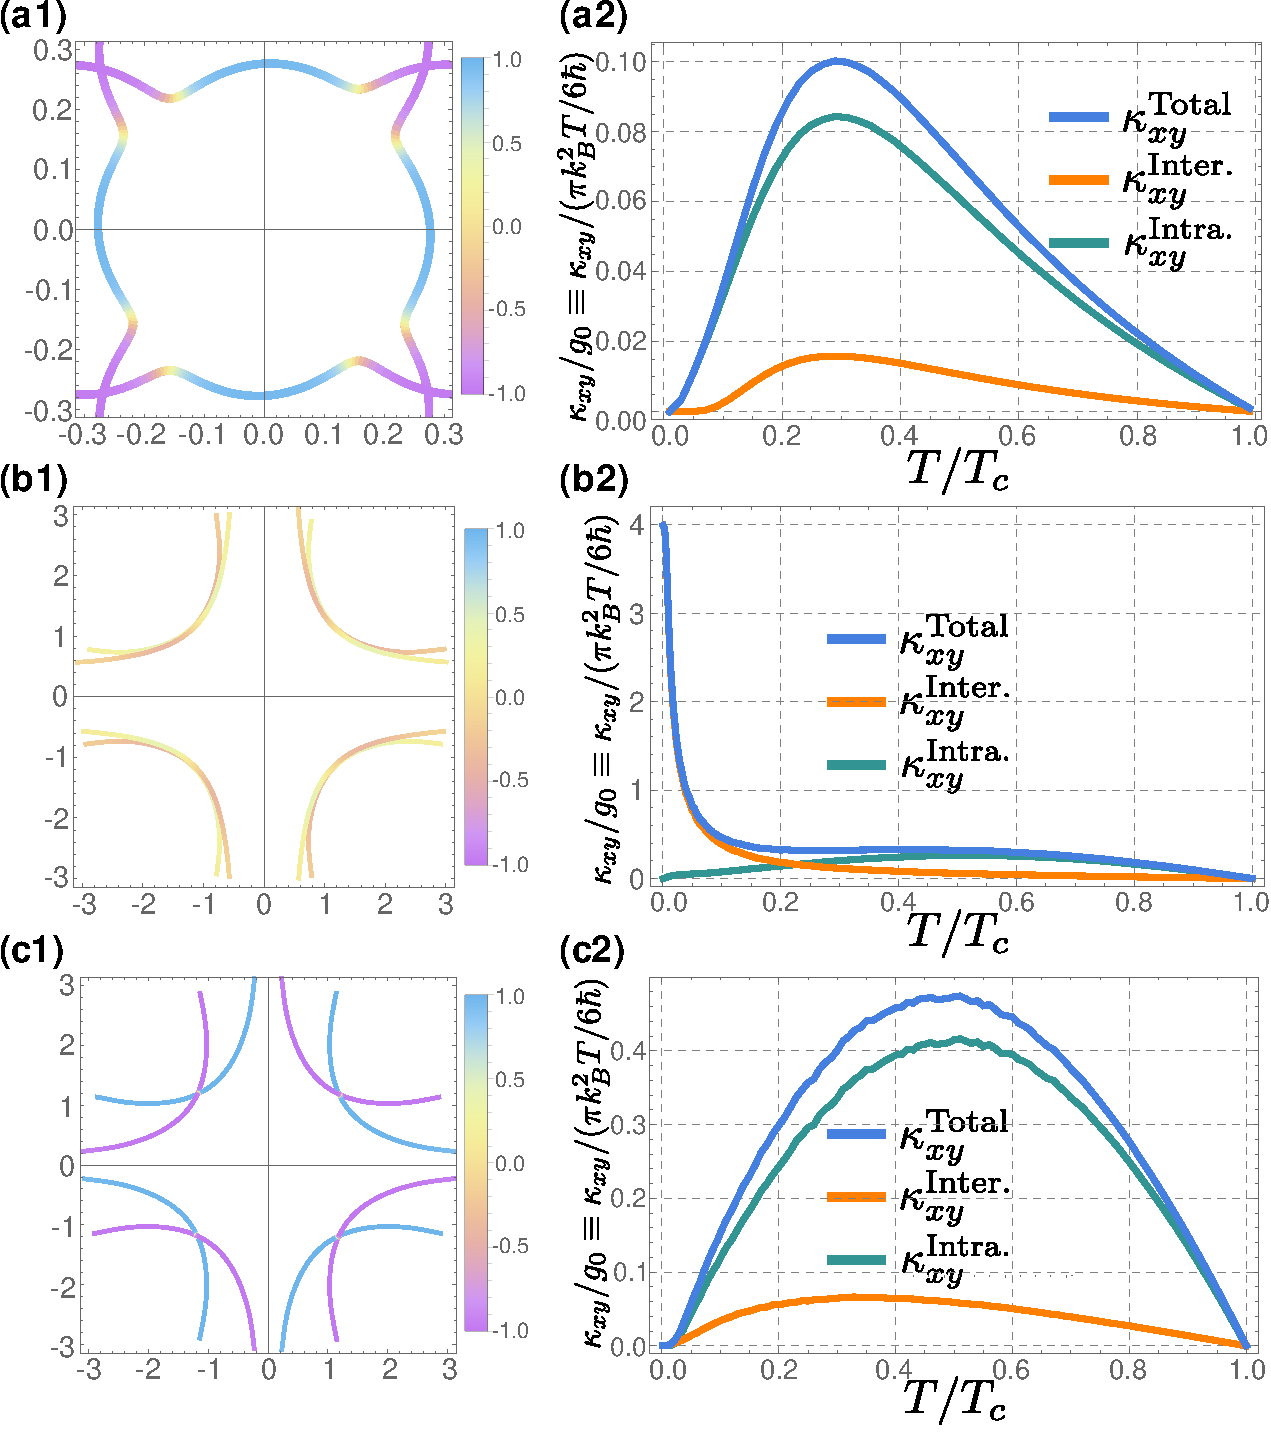
\includegraphics[width=0.85\textwidth]{contents/SATHE/figures/combined.pdf}
	\caption{(a): JJ formed by twisted bilayer FeSe. (b) and (c): the topological non-trivial and trivial phases induced by the supercurrent in JJ formed by twisted bilayer cuprates. The twisted Fermi surfaces are shown on the left panels. For FeSe the moir\'e zone folding effect plays an important role on the topology of reconstructed Fermi surfaces. The color scheme on each Fermi surface represents the strength of $\langle u_{\bm{k}}|\hat{L}|u_{\bm{k}}\rangle\in[-1,1]$, serving as the indicator of the layer-component of states. For all three cases, $\kappa_{xy}$ is computed in unit of the thermal conductance quantum $g_0$ as a function of temperature, and a simple mean-field temperature-dependence of $\varDelta_{\bm{k}}(T)=\varDelta_{\bm{k}}(T=0)\sqrt{1-T/T_c}$ is implemented. For the topologically nontrivial case (b), gaps $\sim 0.2$meV are generated around superconducting nodes, leading to a Chern number $C=8$ topological superconductivity, while for the topological trivial case (c) the net Chern number is zero.}
	\label{fig: FS and kappa_xy}
\end{figure}


\section{Conclusion and Discussion}
We propose the supercurrent-induced anomalous thermal Hall effect, SATHE, as a new probe to the in-plane gap anisotropy of bilayer superconductors. Different from the conventional thermal Hall effect, the ground state preserve the time reversal symmetry. A pair of probes --- a vertically applied supercurrent and a horizontal temperature gradient --- is applied to induce the in-plane nonlinear thermal Hall response. Being a thermal response, it works on 2D superconductors where usual electrical probes fail. Since no external magnetic field needs to be applied, SATHE avoids the complications of vortices in the mixed state and probes purely the quasiparticle dynamics in superconductors. 

Within the BdG framework we showed that SATHE is sensitive to the in-plane gap anisotropy in the twisted bilayer superconductor, and could be large enough to serve as a new experimental probe of gap structure for atomically thin superconducting 2D crystals including twisted bilayer graphene systems, for which experimental probes have been limited due to the low dimensionality. We believe SATHE can eventually find its place as an effective probe of 2D twisted materials, in particular for low $T_c$ superconductors where SATHE can serve as a sensitive measure of the gap anisotropy. 

\begin{subappendices}
\section{The Doppler shift and the gauge transformation due to the supercurrent}
The Doppler shift effect due to supercurrent has been discussed in textbooks and carefully in a recent paper by Crowley and Fu \cite{crowley2022supercurrent}. Below we follow the notation in the Appendix B of Ref. \cite{crowley2022supercurrent}.

To model a superconducting state in the presence of a finite supercurrent with supercurrent velocity $\mathbf u $, it is convenient to consider a moving reference frame $S'$ which is moving at a velocity $\mathbf u$ relative to the lab frame $S$. In the moving frame $S'$, there is no supercurrent and the superconducting order parameter is spatially uniform. 

Microscopically, the Galilean transformation between the frame-$S$ and frame-$S'$ is implemented by the unitary:
\begin{align}
	U_{\mathbf u}&=e^{\frac{i}{\hbar}\mathbf u\cdot \mathbf g},& \mathbf g&=M\mathbf R-\mathbf K t,
\end{align} 
where $\mathbf K$ is the total momentum and $\mathbf R$ is the center of mass:
\begin{align}
	\mathbf K&=\int d\mathbf r\,c_{\mathbf r,\sigma}^\dagger (-i\hbar \nabla) c_{\mathbf r,\sigma},&\mathbf R&=\frac{1}{M}\int d\mathbf r\,c_{\mathbf r,\sigma}^\dagger c_{\mathbf r,\sigma}m \mathbf r.
\end{align}
Here $M$ is the total mass, and $\sigma$ labels electron's spin. Under Galilean transformation, in the real-space basis:
\begin{align}
	U^\dagger_{\mathbf u} c^\dagger_{\mathbf r,\sigma}U_{\mathbf u}=c^\dagger_{\mathbf r-\mathbf u t,\sigma}e^{\frac{-i}{\hbar}m\mathbf r\cdot \mathbf u+\frac{i}{\hbar}m u^2t/2}.
\end{align}
Namely, the electron state $c^\dagger_{\mathbf r,\sigma}$ in frame-$S$ is transformed into the electron state $c^\dagger_{\mathbf r-\mathbf u t,\sigma}$ in frame-$S'$. The \emph{spatially uniform} pairing field in frame-$S'$ then can be represented in the real-space basis:
\begin{align}
	\hat\Delta_{S'}=\int d\mathbf r_1 d\mathbf r_2 \Delta(\mathbf r_1-\mathbf r_2) c^\dagger_{\mathbf r_1-\mathbf u t,\sigma_1}\epsilon_{\sigma_1,\sigma_2} c^\dagger_{\mathbf r_2-\mathbf u t,\sigma_2},
\end{align}
where we assumed spin-singlet pairing for simplicity, and $\epsilon_{\sigma_1,\sigma_2}$ is the Levi-Civita symbol. Performing the inverse Galilean transformation, one finds the pairing field in frame-$S$ is:
\begin{align}
	\hat\Delta_{S}=U_{\mathbf u}\hat\Delta_{S'}U^\dagger_{\mathbf u}=\int d\mathbf r_1 d\mathbf r_2 e^{\frac{i}{\hbar}m(\mathbf r_1+\mathbf r_2)\cdot \mathbf u}\Delta(\mathbf r_1-\mathbf r_2) c^\dagger_{\mathbf r_1,\sigma_1}\epsilon_{\sigma_1,\sigma_2} c^\dagger_{\mathbf r_2,\sigma_2},
\end{align}

One concludes that in the lab frame-$S$, the Cooper pair carries a nonzero center-of-mass momentum $2m\mathbf u$ due to the supercurrent. The mean-field Hamiltonian in the frame-$S$ is given by:
\begin{align}
	H^{MF}_{S}=H_0+\hat\Delta_{S},
\end{align}
where $H_0$ is the normal state Hamiltonian. One may now perform a space-dependent and time-independent gauge transformation $\mathbf U$ (which is different from the Galilean transformation) to eliminate the spatial dependence in the pairing field $\hat\Delta_S$:
\begin{align}
	\mathbf U &= e^{\frac{-i}{\hbar} \int d\mathbf r\,c^\dagger_{\mathbf r,\sigma} c_{\mathbf r,\sigma}m\mathbf r\cdot \mathbf u },& \mathbf U c^\dagger_{\mathbf r,\sigma} \mathbf U^\dagger&= e^{\frac{-i}{\hbar} m\mathbf r\cdot \mathbf u} c^\dagger_{\mathbf r,\sigma}
\end{align}

$H^{MF}_{S}$ after this unitary becomes:
\begin{align}
	\tilde H^{MF}_{S}\equiv \mathbf U H^{MF}_{S} \mathbf U^\dagger= \mathbf U H_0 \mathbf U^\dagger+\int d\mathbf r_1 d\mathbf r_2\Delta(\mathbf r_1-\mathbf r_2) c^\dagger_{\mathbf r_1,\sigma_1}\epsilon_{\sigma_1,\sigma_2} c^\dagger_{\mathbf r_2,\sigma_2},
\end{align}

In $\tilde H^{MF}_{S}$, the pairing field restores the form as if supercurrent is absent, and the normal state Hamiltonian becomes Doppler-shifted due to the gauge transformation. If we denote the phase factor $e^{\frac{-i}{\hbar}m\mathbf r\cdot\mathbf u}\equiv e^{-i\varphi(\mathbf r)/2}$, the supercurrent density is:
\begin{align}
	\mathbf J_s=-e n_s \mathbf u=-e  \frac{\hbar n_s}{2m} \nabla \varphi(\mathbf r),\label{eq:current_relation}
\end{align}
where we introduced the electron's superfluid density $n_s$, and $\varphi (\mathbf r)$ can be identified as the phase of the pairing order parameter, which recovers a well-known result. Generally speaking, the superfluid density may be spatially dependent $n_s(\mathbf r)$. For a uniform supercurrent density, due to current conservation, this implies that the superfluid velocity $\mathbf u(\mathbf r)$ would be spatially dependent. Namely, $\mathbf u(\mathbf r)$, or $\nabla \varphi$, would be larger when $n_s(\mathbf r)$ is smaller. In this situation, the unitary $\mathbf U$ should be modified as:
\begin{align}
	\mathbf U &= e^{\frac{-i}{\hbar} \int d\mathbf r\,c^\dagger_{\mathbf r,\sigma} c_{\mathbf r,\sigma}m \int_{\mathbf 0}^{\mathbf r} d\mathbf r'\cdot \mathbf u(\mathbf r') },& \mathbf U c^\dagger_{\mathbf r,\sigma} \mathbf U^\dagger&= e^{\frac{-i}{\hbar} m\int_{\mathbf 0}^{\mathbf r} d \mathbf r'\cdot \mathbf u(\mathbf r')} c^\dagger_{\mathbf r,\sigma}\equiv e^{-i\varphi(\mathbf r)/2}c^\dagger_{\mathbf r,\sigma},
\end{align}
and one still has $\mathbf u(\mathbf r)=\frac{\hbar}{2m}\nabla \varphi(\mathbf r)$.

The bottom line is that no matter the system is a bilayer Josephson junction or an instrinsic bilayer superconductor, a finite vertical supercurrent state is always modeled by the gauge transformation $c^\dagger_{\mathbf r,\sigma}\rightarrow e^{-i\varphi(\mathbf r)/2} c^\dagger_{\mathbf r,\sigma}$ that transforms the normal state electronic structure $H_0\rightarrow \mathbf U H_0 \mathbf U^\dagger$ while leaving the pairing field spatially uniform (as if the supercurrent is absent), as we have done in Eq.(4) in the main text. Here $\varphi(\mathbf r)$ satisfies Eq.(\ref{eq:current_relation}), and is only depending on the vertical coordinate $z$: $\varphi(\mathbf r)=\varphi(z)$.

The difference between the two cases lies in the details of the profile of $\varphi(z)$. In the case of a bilayer Josephson junction, the superfluid density is concentrated in each monolayers, while between the two layers $n_s$ is small. Consequently, the gradient of the phase $\varphi(z)$ is essentially located between the two layers. In the case of an intrinsic bilayer superconductor, $\varphi(z)$ would be a more smooth function of $z$. We schematically plot the phase $\varphi(z)$ of the gauge transformation for the two cases in Fig.\ref{fig:schematic_phase}.
\begin{figure}\label{fig:schematic_phase}
	\centering
    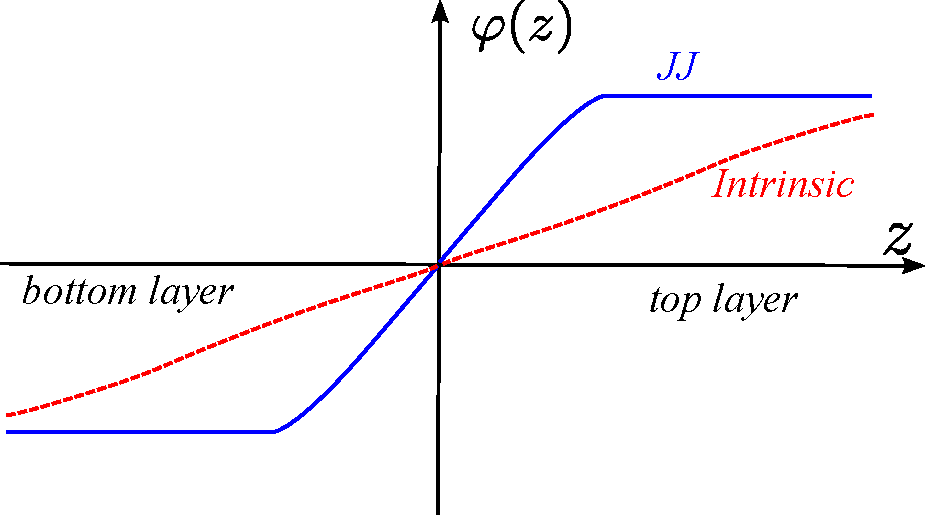
\includegraphics[width=0.4\textwidth]{contents/SATHE/figures/schematic_phase.pdf}
	\caption{The schematic plot of the phase $\varphi$ involved in the gauge transformation to describe a finite supercurrent state. The two curves represent the case of a Josephson junction (JJ) and an intrinsic bilayer superconductor(Intrinisic) respectively.}
\end{figure}

We now consider the situation that $\varphi(z)$ interpolates the top layer $\delta\varphi/2$ to the bottom layer $-\delta\varphi/2$. The Doppler shift unitary is generated via $\hat L$: $\mathbf U=e^{-i\frac{\delta\varphi}{4} \hat L}$. 
\begin{itemize}
	\item In the case of a vertical JJ, $\hat L$ can written in the tight-binding basis, where the $\pm\mathbf 1$ blocks correspond to the top/bottom layers:
	\begin{align}
		\hat L_{\text{JJ}}=\hat c^\dagger \begin{pmatrix} \mathbf{1}&0\\0&\mathbf{-1}\end{pmatrix} c.
	\end{align} 
	\item In the case of an intrinsic bilayer superconductor, assuming the superfluid density is uniform, $\hat L$ is a diagonal matrix whose diagonal matrix elements are given by $\frac{z_\alpha}{z_0}$, where $z_\alpha$ is the atomic coordinate of the orbital-$\alpha$ and $\pm z_0$ is the position of the top/botom layers.
	\begin{align}
		\hat L_{\text{Intrinsic}}=\sum_\alpha c_\alpha^\dagger \frac{z_\alpha}{z_0} c_\alpha
	\end{align}
\end{itemize} 


\section{Details on the Derivation of the Main Result} \label{app:Derivation_Details}

\subsection{Supercurrent-indcued Berry Curvature for Intraband Pairing}
Here we provide details of the derivation of the main result Eq.(1) in the main text. Because only $\mathbf a=\pm 1$ bands contribute to the low-energy Berry curvature, we will start with Eq.(8) in the main text.

Denoting the $c$-th eigenstate of $H_0(\bm{k})$ as $|u^c_{\bm{k}}\rangle$: $H_0(\bm{k})|u^c_{\bm{k}}\rangle=\epsilon_{c,\bm{k}}|u^c_{\bm{k}}\rangle$, and introducing the normal state projector $P_c\equiv |u^c_{\bm{k}}\rangle\langle u^c_{\bm{k}}|$, we can define the BdG projector into the low energy Hilbert space:
\begin{align}
	\mathbf P \equiv P_1\otimes \boldsymbol \tau_0,
\end{align}
where $\boldsymbol \tau_0$ is the identity Pauli matrix in the particle-hole space.
The low-energy BdG Hamiltonian is simply the two-by-two matrix, which perfectly decouples from the high energy Hilbert space if only intraband pairing is present (which we call \emph{intraband pairing assumption} below):
\begin{align}
	\mathbf P \mathbf H \mathbf P= P_1\otimes (\epsilon_{1,\bm{k}}\boldsymbol\tau_3+\varDelta_{\bm{k}}\boldsymbol\tau_1).
\end{align}
Here $\varDelta_{\bm{k}}$ is chosen to be real due to the time-reversal symmetry. In addition, Projector $\mathbf P$ satisfies an important identity with any operator of the following form:
\begin{align}
	\mathbf A^\vee\equiv A \otimes \boldsymbol\tau_0 \Rightarrow \mathbf P\mathbf A\mathbf P=\langle u^1_{\bm{k}}|A|u^1_{\bm{k}}\rangle\mathbf P,
\end{align}
which in turn indicates $\mathbf P_{-\mathbf a}\mathbf{A^\vee} \mathbf P_{\mathbf a}=0$.

After the pairing phase twist $\delta \varphi$ are turned on, $\mathbf H, \mathbf E_{\pm\mathbf a}, \mathbf P_{\pm \mathbf a}$ all receive perturbations in Eq.(8) in the main text. $\delta\mathbf H$ and $\delta\mathbf E_{\pm\mathbf a}$ do not contribute because $\partial_\varphi\mathbf H$ and $\partial_{k_x}\partial_\varphi\mathbf H$ both have the form of $\mathbf A^\vee$ \emph{under the intraband assumption}. For instance:
\begin{align}
	\partial_\varphi \mathbf H=\partial_\varphi H_0(\bm{k})\otimes\boldsymbol\tau_0\label{eq:partial_varphi}.
\end{align}
Thus we are left with the $\delta \mathbf P_{\pm \mathbf a}$ contribution only:
\begin{align}
\frac{\delta \boldsymbol \Omega ^{\mathbf a}}{\delta \varphi}\doteq \frac{- \mbox{Im\,Tr}[\mathbf P_{\mathbf a} \partial_{k_x} \mathbf H \mathbf P_{-\mathbf a} \partial_{k_y}\mathbf H \partial_\varphi\mathbf P_{\mathbf a}]}{\mathbf E_{\mathbf a}^2}-(x\leftrightarrow y).
\end{align}
Here we used the time-reversal symmetry combined with the particle-hole symmetry, which dictates that the $\delta \mathbf P_{-\mathbf a}$ contribution and $\delta \mathbf P_{\mathbf a}$ contribution are identical. After inserting $\mathbf 1=\sum_{\mathbf c} \mathbf{P}_{\mathbf c}$ in front of $\partial_\varphi \mathbf P_{\mathbf a}$, and noting that only terms with $\mathbf c\neq \pm \mathbf a$ contributes \emph{under the intraband pairing assumption}, the above expression can be rewritten as:
\begin{align}
	\frac{\delta \boldsymbol \Omega ^{\mathbf a}}{\delta \varphi}\doteq &\sum_{\mathbf b\neq \pm\mathbf a}\frac{\mbox{Im\,Tr}[\mathbf P_{\mathbf a} \partial_{k_x} \mathbf H \mathbf P_{-\mathbf a} \partial_{k_y}\mathbf H \mathbf P_{\mathbf b}\partial_\varphi\mathbf H \mathbf P_{\mathbf a}]}{\mathbf E_{\mathbf a}^2(\mathbf E_{\mathbf b}-\mathbf E_{\mathbf a})}-(x\leftrightarrow y)\notag\\
	=&\sum_{\mathbf b\neq \pm\mathbf a}\frac{ \mbox{Im\,Tr}[\mathbf P_{\mathbf a} \partial_{k_x} \mathbf H \mathbf P_{-\mathbf a} \partial_{k_y}\mathbf P_{\mathbf b}\partial_\varphi\mathbf H \mathbf P_{\mathbf a}]}{\mathbf E_{\mathbf a}^2(\mathbf E_{\mathbf b}-\mathbf E_{\mathbf a})}(\mathbf E_{\mathbf b}+\mathbf E_{\mathbf a})-(x\leftrightarrow y)\notag\\
	=&\sum_{\mathbf b\neq \pm\mathbf a}\frac{2 \mbox{Im\,Tr}[\mathbf P_{\mathbf a} \partial_{k_x} \mathbf H \mathbf P_{-\mathbf a} \partial_{k_y}\mathbf P_{\mathbf b}\partial_\varphi\mathbf H \mathbf P_{\mathbf a}]}{\mathbf E_{\mathbf a}(\mathbf E_{\mathbf b}-\mathbf E_{\mathbf a})}-(x\leftrightarrow y)\notag\\
	&\qquad+\sum_{\mathbf b\neq \pm\mathbf a}\frac{ \mbox{Im\,Tr}[\mathbf P_{\mathbf a} \partial_{k_x} \mathbf H \mathbf P_{-\mathbf a} \partial_{k_y}\mathbf P_{\mathbf b}\partial_\varphi\mathbf H \mathbf P_{\mathbf a}]}{\mathbf E_{\mathbf a}^2}-(x\leftrightarrow y).\label{eq:Omega_middle}
\end{align}
The term in the last line vanishes \emph{under the intraband pairing assumption}: $\mathbf P =\mathbf P_1+\mathbf P_{-1}$, $\sum_{\mathbf b\neq \pm\mathbf a}\partial_{k_y}\mathbf P_{\mathbf b}=-\partial_{k_y}\mathbf P$, and the fact that $\partial_{k_y}\mathbf P\partial_\varphi \mathbf H$ takes the form of $\mathbf A^\vee$. We therefore arrive at:
\begin{align}
	\frac{\delta \boldsymbol \Omega ^{\mathbf a,\text{intra.}}}{\delta \varphi}\doteq&\sum_{\mathbf b\neq \pm\mathbf a}4 \mbox{Im\,Tr}[\partial_{k_x}\mathbf P_{\mathbf a}  \partial_{k_y}\mathbf P_{-\mathbf a} \mathbf P_{\mathbf b}\partial_\varphi\mathbf P_{\mathbf a}\mathbf P_{\mathbf a}]-(x\leftrightarrow y)\notag\\
	=&\sum_{\mathbf b\neq \pm\mathbf a}\frac{2 \mbox{Im\,Tr}[\mathbf P_{\mathbf a} \partial_{k_x}\mathbf H \mathbf P_{-\mathbf a} \partial_{k_y}\mathbf H\mathbf P_{\mathbf b}\partial_\varphi\mathbf H\mathbf P_{\mathbf a}]}{ \mathbf E_{\mathbf a} (\mathbf E_{\mathbf b}-\mathbf E_{\mathbf a})(\mathbf E_{\mathbf b}-\mathbf E_{-\mathbf a})}-(x\leftrightarrow y)\notag\\
	\doteq &\sum_{b\neq 1}\frac{2 \mbox{Im\,Tr}[\mathbf P_{\mathbf a} \partial_{k_x}\mathbf H \mathbf P_{-\mathbf a} \partial_{k_y}\mathbf H(\mathbf P_{b}+\mathbf P_{-b})\partial_\varphi\mathbf H\mathbf P_{\mathbf a}]}{ \mathbf E_{\mathbf a} (\epsilon_{b}-\epsilon_{1})^2}-(x\leftrightarrow y)\notag\\
	= &\sum_{b\neq 1}\frac{2 \mbox{Im\,Tr}[\mathbf P_{\mathbf a} \partial_{k_x}\mathbf H \mathbf P_{-\mathbf a} \partial_{k_y}\mathbf H P_b\otimes\boldsymbol\tau_0 \partial_\varphi\mathbf H\mathbf P_{\mathbf a}]}{ \mathbf E_{\mathbf a} (\epsilon_{b}-\epsilon_{1})^2}-(x\leftrightarrow y)
\end{align}

Now we are ready to connect with the properties of the normal state. Introducing two-dimensional eigenvectors $|\boldsymbol\alpha_\mathbf c\rangle$ in the particle-hole subspace:
\begin{align}
	|\mathbf u^{\mathbf c}_{\bm{k}}\rangle=|u^{|\mathbf c|}_{\bm{k}}\rangle\otimes|\boldsymbol\alpha_\mathbf c \rangle,
\end{align}
and noting that
\begin{align}
	\partial_{k}\mathbf H=\partial_{\bm{k}} H_0(\bm{k})\otimes\boldsymbol\tau_3+O(\partial_{\bm{k}}\boldsymbol\Delta_{\bm{k}}),\label{eq:partial_k}
\end{align}
together with Eq.(\ref{eq:partial_varphi}), one has:
\begin{align}
	\frac{\delta \boldsymbol \Omega ^{\mathbf a,\text{intra.}}}{\delta \varphi}\doteq &\sum_{b\neq 1}\frac{2 |\langle \boldsymbol\alpha_\mathbf a|\tau_3| \boldsymbol\alpha_{-\mathbf a}\rangle|^2 \mbox{Im\,Tr}[P_1 \partial_{k_x}H_0 P_1 \partial_{k_y} H_0 P_b \partial_\varphi H_0 P_1]}{ \mathbf E_{\mathbf a} (\epsilon_{b}-\epsilon_{1})^2}-(x\leftrightarrow y)\notag\\
	=&\sum_{b\neq 1}\frac{2 |\langle \boldsymbol\alpha_\mathbf a|\tau_3| \boldsymbol\alpha_{-\mathbf a}\rangle|^2 v_x \mbox{Im\,Tr}[ P_1 \partial_{k_y} H_0 P_b \partial_\varphi H_0 P_1]}{ \mathbf E_{\mathbf a} (\epsilon_{b}-\epsilon_{1})^2}-(x\leftrightarrow y)\notag\\
	=&- \frac{v_x|\langle \boldsymbol\alpha_\mathbf a|\tau_3| \boldsymbol\alpha_{-\mathbf a}\rangle|^2     }{\mathbf E_{\mathbf a}}\Omega_{k_y,\varphi}-(x\leftrightarrow y)=- \frac{\varDelta_{\bm{k}}^2}{\mathbf E_{\mathbf a}^3}v_x  \Omega_{k_y,\varphi}-(x\leftrightarrow y),
\end{align}
where $v_x\equiv \partial_{k_x} \epsilon_{1,\bm{k}}$, and $\Omega_{k_y,\varphi}\equiv -2\mbox{Im}[\langle\partial_{k_y} u^1_{\bm{k}}|\partial_\varphi u^1_{\bm{k}}\rangle]$ is the \emph{normal-state} Berry curvature w.r.t. $k_y$ and $\varphi$. Using the fact that $|\partial_\varphi u^1_{\bm{k}}\rangle=\frac{-i}{4}\hat L |u^1_{\bm{k}}\rangle$, the normal-state Berry curvature $\Omega_{k,\varphi}$ can also be expressed as
\begin{align}
	\Omega_{k,\varphi}=\frac{1}{4}\partial_{\bm{k}}\langle u^1_{\bm{k}}|\hat L|u^1_{\bm{k}}\rangle,
\end{align}
so that Eq.(10) in the main text is obtained.


\subsection{Fermi Surface Integral}
The SATHE can be computed using Eq.(5) and Eq.(6) in the main text. Define
\begin{align}
	\boldsymbol\Omega(E)\equiv \sum_{\mathbf a}\int \frac{d^2k}{(2\pi)^2}\boldsymbol\Omega^\mathbf a_{\bm{k}}\delta(E-\mathbf E_{\mathbf a,\bm{k}}),
\end{align}
we have $\boldsymbol\sigma (E)=\boldsymbol\sigma(0)-\int_0^E dE'\boldsymbol\Omega(E')$. Here $\boldsymbol\sigma(0)=0$ due to the time-reversal symmetry and the nodeless assumption.

Because the change of the Berry curvature is concentrated near the Fermi surface due to the $\mathbf E_{\mathbf a}$ denominator, and proportional to $1/\varDelta_{\bm{k}}$ right at the Fermi surface, it is convenient to represent $\boldsymbol\Omega(E)$ as a Fermi surface integral as following:
\begin{align}
	\frac{\delta\boldsymbol\Omega(E)}{\delta\varphi}
	\doteq &\sum_{\text{FS}}\frac{1}{(2\pi)^2}\oint _{\text{FS},\epsilon_{\bm{k}}\equiv\pm\sqrt{E^2-\varDelta_{\bm{k}}^2}} dk_\parallel \frac{|E|}{|\epsilon_{\bm{k}}|}\frac{1}{\hbar |v_F|}\mathbf\Omega^{\mathop{\mathrm{sign}}(E)}_{\bm{k}}\notag\\
	\doteq &\sum_{\text{FS}}\frac{-2}{(2\pi)^2}\oint _{\text{FS}} dk_\parallel \frac{|E|}{\sqrt{E^2-\varDelta_{\bm{k}}^2}}\frac{1}{\hbar |v_F|}\frac{\varDelta_{\bm{k}}^2}{E^3}(v_x\Omega_{k_y,\varphi}-v_y\Omega_{k_x,\varphi})\notag\\
	=&\mathop{\mathrm{sign}}(E)\sum_{\text{FS}}\frac{-1}{2\pi^2}\oint _{\text{FS}} dk_\parallel \frac{\varDelta_{\bm{k}}^2}{E^2\sqrt{E^2-\varDelta_{\bm{k}}^2}}\frac{1}{\hbar |v_F|}(v_x\Omega_{k_y,\varphi}-v_y\Omega_{k_x,\varphi})\notag\\
	=&\mathop{\mathrm{sign}}(E)\sum_{\text{FS}}\frac{-\mathop{\mathrm{sign}}(v_F)}{2\pi^2\hbar}\oint _{\text{FS}} d\vec k_\parallel \cdot (\Omega_{k_x,\varphi},\Omega_{k_y,\varphi}) \frac{\varDelta_{\bm{k}}^2}{E^2\sqrt{E^2-\varDelta_{\bm{k}}^2}}\notag\\
	=&\mathop{\mathrm{sign}}(E)\sum_{\text{FS}}\frac{-\mathop{\mathrm{sign}}(v_F)}{8\pi^2\hbar}\oint _{\text{FS}} d k_\parallel \partial_{k_\parallel} \langle u_{\bm{k}}|\hat L|u_{\bm{k}} \rangle \frac{\varDelta_{\bm{k}}^2}{E^2\sqrt{E^2-\varDelta_{\bm{k}}^2}}.
\end{align}

Integrating out $E$ in advance, we get
\begin{align}
	\boldsymbol\sigma(E)=\sum_{\text{FS}}\frac{\mathop{\mathrm{sign}}(v_F)}{8\pi^2\hbar}\oint _{\text{FS}} d k_\parallel \partial_{k_\parallel} \langle u_{\bm{k}}|\hat L|u_{\bm{k}} \rangle \frac{\sqrt{E^2-\varDelta_{\bm{k}}^2}}{|E|}\Theta(|E|-|\varDelta_{\bm{k}}|).
\end{align}

We finally arrive at the result using Eq.(5) in the main text:
\begin{align}
	\frac{\delta\kappa_{xy}}{\delta\varphi T}=\sum_{\text{FS}}\frac{\mathop{\mathrm{sign}}(v_F)k_B^2}{16\pi^2\hbar}\oint _{\text{FS}} d k_\parallel \partial_{k_\parallel} \langle u_{\bm{k}}|\hat L|u_{\bm{k}} \rangle \xi\bigg(\frac{\varDelta_{\bm{k}}}{T}\bigg).
\end{align}



\section{Supercurrent-indcued Berry Curvature for Interband Pairing}
When interband pairing is present, additional terms need to be considered. However, one can always perform a small unitary rotation $e^{iS\otimes\boldsymbol\tau_2}$ to eliminate the interband pairing:
\begin{align}
	S\equiv \sum_{a\neq b}\frac{P_a\boldsymbol \Delta^{\text{inter.}}_{\bm{k}} P_b}{\epsilon_{a,\bm{k}}+\epsilon_{b,\bm{k}}}, \quad S^\dagger=S.
\end{align}
Since $\mathbf H = H_0\otimes\boldsymbol\tau_3+ (\boldsymbol \Delta^{\text{intra.}}+\boldsymbol\Delta^{\text{inter.}})\otimes \boldsymbol \tau_1$, we have:
\begin{align}
	e^{iS\otimes\boldsymbol\tau_2}\mathbf H e^{-iS\otimes\boldsymbol\tau_2}\doteq & H_0\otimes\boldsymbol\tau_3+(\boldsymbol \Delta^{\text{intra.}}+\boldsymbol\Delta^{\text{inter.}})\otimes \boldsymbol \tau_1+(i)[S\otimes\boldsymbol\tau_2,H_0\otimes\boldsymbol\tau_3]\notag\\
	=& H_0\otimes\boldsymbol\tau_3+(\boldsymbol \Delta^{\text{intra.}}+\boldsymbol\Delta^{\text{inter.}})\otimes \boldsymbol \tau_1+(i) (SH_0+H_0S)\otimes (i)\boldsymbol\tau_1\notag\\
	=&H_0\otimes\boldsymbol\tau_3+(\boldsymbol \Delta^{\text{intra.}}+\boldsymbol\Delta^{\text{inter.}})\otimes \boldsymbol \tau_1+(-1) \boldsymbol\Delta^{\text{inter.}}_{\bm{k}}\otimes \boldsymbol\tau_1\notag\\
    =&H_0\otimes\boldsymbol\tau_3+\boldsymbol \Delta^{\text{intra.}}\otimes \boldsymbol \tau_1
\end{align}

Denoting the projectors in the presence of interband pairing as $\widetilde {\mathbf P}_{\mathbf c}$, we have $\widetilde {\mathbf P}_{\mathbf c}\doteq e^{-i S\otimes\boldsymbol\tau_2}\mathbf P_{\mathbf c}e^{i S\otimes\boldsymbol\tau_2}$. Basically, in all the previous derivations for the intraband case, we only need to replace $\mathbf P_{\mathbf c}$ by $\widetilde {\mathbf P}_{\mathbf c}$, which corresponds to performing the small unitary transformation for the operators like $\partial_\varphi\mathbf H\rightarrow e^{i S\otimes\boldsymbol\tau_2}\partial_\varphi\mathbf H e^{-i S\otimes\boldsymbol\tau_2}$. In this way $\partial_\varphi \mathbf H$ has a correction $[i S, \partial_\varphi H_0]\otimes\boldsymbol\tau_2$ and is no longer $\propto \boldsymbol\tau_0$. We can leave all the energies $\mathbf E_{\mathbf c}$ unchanged since they receive second order contributions from $\boldsymbol\Delta^{\text{inter.}}$.

After inspection, to the leading order of $\varDelta/t$, one can identify three sources of interband contributions. First, we do need to consider $\delta_\varphi \partial_{\bm{k}} \mathbf H$ in Eq.(8) in the main text. Second, in the first line of Eq.(\ref{eq:Omega_middle}), $\mathbf b=-\mathbf a$ needs to be included. Third, the term in the last line of Eq.(\ref{eq:Omega_middle}) is no longer vanishing. We term them as \emph{Part-A,B,C} and compute them one by one below.

\emph{Part-A:} For the $\delta_\varphi \partial_{\bm{k}} \mathbf H$ contributions, 
\begin{align}
	\left.\frac{\delta\boldsymbol\Omega^{\mathbf a}_{\bm{k}}}{\delta\varphi}\right|_{A} 
    &= \frac{-\mbox{Im\,Tr}\big[\mathbf P_{\mathbf a}\partial_{k_x}\mathbf H \mathbf P_{-\mathbf a} [iS\otimes\boldsymbol\tau_2,\partial_{k_y}\partial_{\varphi}\mathbf H] \mathbf P_{\mathbf a}\big]}{2\mathbf E^2_{\mathbf a}}-(x\leftrightarrow y)\notag\\
	&=\frac{-\mbox{Im\,Tr}\big[\mathbf P_{\mathbf a}(\partial_{k_x}H_0\otimes\boldsymbol\tau_3 +\partial_{k_x}\boldsymbol\Delta\otimes\boldsymbol\tau_1 ) \mathbf P_{-\mathbf a} [iS\otimes\boldsymbol\tau_2,\partial_{k_y}\partial_{\varphi}H_0\otimes\boldsymbol\tau_0] \mathbf P_{\mathbf a}\big]}{2\mathbf E^2_{\mathbf a}}\notag\\
    &\qquad-(x\leftrightarrow y)\notag\\
	&=-\langle u^1_{\bm{k}}|[iS,\partial_{k_y}\partial_{\varphi}H_0]|u^1_{\bm{k}}\rangle\notag\\
    &\qquad\times\frac{v_x\mbox{Im}\big[\langle\boldsymbol\alpha_{\mathbf a}|\boldsymbol\tau_3  |\boldsymbol\alpha_{-\mathbf a}\rangle\langle\boldsymbol\alpha_{-\mathbf a}|\boldsymbol\tau_2 |\boldsymbol\alpha_{\mathbf a}\rangle\big]+\langle u^1_{\bm{k}}|\partial_{k_x}\boldsymbol\Delta|u^1_{\bm{k}}\rangle \mbox{Im}\big[\langle\boldsymbol\alpha_{\mathbf a}|\boldsymbol\tau_1  |\boldsymbol\alpha_{-\mathbf a}\rangle\langle\boldsymbol\alpha_{-\mathbf a}|\boldsymbol\tau_2 |\boldsymbol\alpha_{\mathbf a}\rangle\big]}{2\mathbf E^2_{\mathbf a}}\notag\\
    &\qquad-(x\leftrightarrow y).
\end{align}
Noting a few identities:
\begin{align}
	&\boldsymbol\tau_2|\boldsymbol\alpha_{-\mathbf a}\rangle\langle\boldsymbol\alpha_{-\mathbf a}|\boldsymbol\tau_2=|\boldsymbol\alpha_{\mathbf a}\rangle\langle\boldsymbol\alpha_{\mathbf a}|\notag\\  
	&\partial_{k_x}\mathbf E_\mathbf a=\mbox{Tr}[\mathbf P_\mathbf a (\partial_{k_x} H_0\otimes \boldsymbol \tau_3+\partial_{k_x} \boldsymbol\Delta\otimes \boldsymbol \tau_1)\mathbf P_\mathbf a]=v_x \frac{\epsilon_{1,\bm{k}}}{\mathbf E_a}+\langle u^1_{\bm{k}}|\partial_{k_x}\boldsymbol\Delta|u^1_{\bm{k}}\rangle \frac{\varDelta_{\bm{k}}}{\mathbf E_\mathbf a}\notag\\
	&\partial_{k_x} \mathbf E_\mathbf a=\frac{\varDelta_{\bm{k}}\partial_{k_x}\varDelta_{\bm{k}}+\epsilon_{1,\bm{k}}v_x}{\mathbf E_\mathbf a}\notag\\
	&\Rightarrow \langle u^1_{\bm{k}}|\partial_{k_x}\boldsymbol\Delta|u^1_{\bm{k}}\rangle = \partial_{k_x}\varDelta_{\bm{k}}\notag\\
	&\langle\boldsymbol\alpha_{\mathbf a}|\boldsymbol\tau_1  |\boldsymbol\alpha_{\mathbf a}\rangle=\frac{\varDelta_{\bm{k}}}{\mathbf E_\mathbf a}, \;\;\langle\boldsymbol\alpha_{\mathbf a}|\boldsymbol\tau_3  |\boldsymbol\alpha_{\mathbf a}\rangle=\frac{\epsilon_{1,\bm{k}}}{\mathbf E_\mathbf a}
\end{align}
we have:
\begin{align}
	\left.\frac{\delta\boldsymbol\Omega^{\mathbf a}_{\bm{k}}}{\delta\varphi}\right|_{A}
	=&-\frac{\langle u^1_{\bm{k}}|[iS,\partial_{k_y}\partial_{\varphi}H_0]|u^1_{\bm{k}}\rangle}{2\mathbf E^3_{\mathbf a}}\big(-\varDelta_{\bm{k}} v_x+\epsilon_{1,\bm{k}}\partial_{k_x}\varDelta_{\bm{k}}\big)-(x\leftrightarrow y)\notag\\
\end{align}

\emph{Part-B:} This term is:
\begin{equation}
	\frac{\mbox{Im\,Tr}[\mathbf P_{\mathbf a} \partial_{k_x} \mathbf H \mathbf P_{-\mathbf a} \partial_{k_y}\mathbf H \mathbf P_{-\mathbf a}\partial_\varphi\mathbf H \mathbf P_{\mathbf a}]}{\mathbf E_{\mathbf a}^2(\mathbf E_{-\mathbf a}-\mathbf E_{\mathbf a})}-(x\leftrightarrow y)
\end{equation}
Note that $\mathbf P_{-\mathbf a} \partial_{k_y}\mathbf H \mathbf P_{-\mathbf a}=\partial_{k_y}\mathbf E_{\mathbf -a}\mathbf P_{-\mathbf a}$,
\begin{align}
	\left.\frac{\delta\boldsymbol\Omega^{\mathbf a}_{\bm{k}}}{\delta\varphi}\right|_{B}=&\frac{\partial_{k_y}\mathbf E_{\mathbf a}}{2\mathbf E_{\mathbf a}^3}\mbox{Im\,Tr}[\mathbf P_{\mathbf a} (\partial_{k_x}H_0\otimes\boldsymbol\tau_3+\partial_{k_x}\boldsymbol\Delta\otimes\boldsymbol\tau_1) \mathbf P_{-\mathbf a} [iS,\partial_\varphi H_0]\otimes\boldsymbol\tau_2 \mathbf P_{\mathbf a}]-(x\leftrightarrow y)\notag\\
	=&\frac{\partial_{k_y}\mathbf E_{\mathbf a}}{2\mathbf E_{\mathbf a}^3}\langle u^1_{\bm{k}}|[iS,\partial_\varphi H_0]|u^1_{\bm{k}}\rangle\mbox{Im\,Tr}[\mathbf P_{\mathbf a} (\partial_{k_x}H_0\otimes\boldsymbol\tau_3+\partial_{k_x}\boldsymbol\Delta\otimes\boldsymbol\tau_1) \mathbf P_{-\mathbf a}\boldsymbol\tau_2 \mathbf P_{\mathbf a}]  -(x\leftrightarrow y)\notag\\
	=&\frac{\partial_{k_y}\mathbf E_{\mathbf a}}{2\mathbf E_{\mathbf a}^3}\langle u^1_{\bm{k}}|[iS,\partial_\varphi H_0]|u^1_{\bm{k}}\rangle\mbox{Im\,Tr}[\mathbf P_{\mathbf a} (\partial_{k_x}H_0\otimes\boldsymbol\tau_3+\partial_{k_x}\boldsymbol\Delta\otimes\boldsymbol\tau_1) \boldsymbol\tau_2 \mathbf P_{\mathbf a}]  -(x\leftrightarrow y)\notag\\
	=&\frac{\partial_{k_y}\mathbf E_{\mathbf a}}{2\mathbf E_{\mathbf a}^3}\langle u^1_{\bm{k}}|[iS,\partial_\varphi H_0]|u^1_{\bm{k}}\rangle (-v_x\langle\boldsymbol\alpha_{\mathbf a}|\boldsymbol\tau_1| \boldsymbol\alpha_{\mathbf a}\rangle + \langle u^1_{\bm{k}}|\partial_{k_x}\boldsymbol\Delta|u^1_{\bm{k}}\rangle \langle\boldsymbol\alpha_{\mathbf a}|\boldsymbol\tau_3| \boldsymbol\alpha_{\mathbf a}\rangle ) -(x\leftrightarrow y)\notag\\
	=&\frac{\partial_{k_y}\mathbf E_{\mathbf a}}{2\mathbf E_{\mathbf a}^4}\langle u^1_{\bm{k}}|[iS,\partial_\varphi H_0]|u^1_{\bm{k}}\rangle \big(-\varDelta_{\bm{k}} v_x+\epsilon_{1,\bm{k}}\partial_{k_x}\varDelta_{\bm{k}}\big) -(x\leftrightarrow y)\notag\\
	=&\frac{(v_y\epsilon_{1,\bm{k}}+\varDelta_{\bm{k}}\partial_{k_y}\varDelta_{\bm{k}})}{2\mathbf E_{\mathbf a}^5}\langle u^1_{\bm{k}}|[iS,\partial_\varphi H_0]|u^1_{\bm{k}}\rangle \big(-\varDelta_{\bm{k}} v_x+\epsilon_{1,\bm{k}}\partial_{k_x}\varDelta_{\bm{k}}\big) -(x\leftrightarrow y)
\end{align}
After $(x\leftrightarrow y)$ antisymmetrization, we get
\begin{align}
	\left.\frac{\delta\boldsymbol\Omega^{\mathbf a}_{\bm{k}}}{\delta\varphi}\right|_{B}=&\frac{-1}{2\mathbf E_{\mathbf a}^3}\langle u^1_{\bm{k}}|[iS,\partial_\varphi H_0]|u^1_{\bm{k}}\rangle v_x\partial_{k_y}\varDelta_{\bm{k}} -(x\leftrightarrow y)
\end{align}

\emph{Part-C:} Note that 
\begin{align}
\partial_{k_y} \widetilde{\mathbf P}_{\mathbf b}\doteq \partial_{k_y}\big[\mathbf P_{\mathbf b}+[-i S\otimes\boldsymbol\tau_2,\mathbf P_{\mathbf b}]\big]\doteq e^{-i S\otimes\boldsymbol\tau_2}\partial_{k_y}\mathbf P_{\mathbf b}e^{i S\otimes\boldsymbol\tau_2}+[-i \partial_{k_y}S\otimes\boldsymbol\tau_2,\mathbf P_{\mathbf b}]
\end{align}
The contribution from the last line of Eq.(\ref{eq:Omega_middle}) becomes:
\begin{align}
	\left.\frac{\delta\boldsymbol\Omega^{\mathbf a}_{\bm{k}}}{\delta\varphi}\right|_{C} 
    &\doteq \frac{ -\mbox{Im\,Tr}[\mathbf P_{\mathbf a} \partial_{k_x} \mathbf H \mathbf P_{-\mathbf a} \partial_{k_y}\mathbf P [iS\otimes \boldsymbol\tau_2,\partial_\varphi\mathbf H] \mathbf P_{\mathbf a}+\mathbf P_{\mathbf a} \partial_{k_x} \mathbf H \mathbf P_{-\mathbf a} [-i \partial_{k_y}S\otimes\boldsymbol\tau_2,\mathbf P]\partial_\varphi\mathbf H \mathbf P_{\mathbf a}]}{\mathbf E_{\mathbf a}^2}\notag\\
    &\qquad-(x\leftrightarrow y)\notag\\
	&=\frac{-1}{\mathbf E_{\mathbf a}^3}\big(-\varDelta_{\bm{k}} v_x+\epsilon_{1,\bm{k}}\partial_{k_x}\varDelta_{\bm{k}}\big)\mbox{Re\,Tr}[\partial_{k_y}P_1[iS,\partial_\varphi H_0]P_1+P_1 i\partial_{k_y}S \partial_\varphi H_0 P_1]\notag\\
    &\qquad-(x\leftrightarrow y)\notag\\
	&=\frac{-1}{2\mathbf E_{\mathbf a}^3}\big(-\varDelta_{\bm{k}} v_x+\epsilon_{1,\bm{k}}\partial_{k_x}\varDelta_{\bm{k}}\big)\mbox{Re\,Tr}[2\partial_{k_y}P_1[iS,\partial_\varphi H_0]P_1+P_1 [i\partial_{k_y}S ,\partial_\varphi H_0] P_1]\notag\\
    &\qquad-(x\leftrightarrow y)
\end{align}

Let's add part-A and part-C together. 
\begin{align}
	\left.\frac{\delta\boldsymbol\Omega^{\mathbf a}_{\bm{k}}}{\delta\varphi}\right|_{A+C}=&\frac{-1}{2\mathbf E_{\mathbf a}^3}\big(-\varDelta_{\bm{k}} v_x+\epsilon_{1,\bm{k}}\partial_{k_x}\varDelta_{\bm{k}}\big)\partial_{k_y}\Big[\mbox{Re\,Tr}[P_1[iS,\partial_\varphi H_0]P_1]\Big]-(x\leftrightarrow y)\notag\\
	=&\frac{-1}{2\mathbf E_{\mathbf a}^3}\big(-\varDelta_{\bm{k}} v_x+\epsilon_{1,\bm{k}}\partial_{k_x}\varDelta_{\bm{k}}\big)\partial_{k_y}\langle u^1_{\bm{k}}|[iS,\partial_\varphi H_0]|u^1_{\bm{k}}\rangle-(x\leftrightarrow y)
\end{align}
The quantity $\langle u^1_{\bm{k}}|[iS,\partial_\varphi H_0]|u^1_{\bm{k}}\rangle$ here and in part-B can be easily computed, which we denote as $G_{\bm{k}}$:
\begin{align}
	G_{\bm{k}}\equiv&\langle u^1_{\bm{k}}|[iS,\partial_\varphi H_0]|u^1_{\bm{k}}\rangle=-2\mbox{Im}[\langle u^1_{\bm{k}}| S \partial_\varphi H_0|u^1_{\bm{k}}\rangle]=-2\sum_{b\neq 1}\mbox{Im}[\langle u^1_{\bm{k}}| S |u^b_{\bm{k}}\rangle\langle u^b_{\bm{k}}|\partial_\varphi H_0|u^1_{\bm{k}}\rangle]\notag\\
	&=-2\sum_{b\neq 1}\mbox{Im}\Big[\frac{\langle u^1_{\bm{k}}| \boldsymbol\Delta^{\text{inter.}} |u^b_{\bm{k}}\rangle\langle u^b_{\bm{k}}|\partial_\varphi H_0|u^1_{\bm{k}}\rangle}{\epsilon_{1,\bm{k}}+\epsilon_{b,\bm{k}}}\Big]\doteq-2\sum_{b\neq 1}\mbox{Im}\Big[\frac{\langle u^1_{\bm{k}}| \boldsymbol\Delta^{\text{inter.}} |u^b_{\bm{k}}\rangle\langle u^b_{\bm{k}}|\partial_\varphi H_0|u^1_{\bm{k}}\rangle}{-\epsilon_{1,\bm{k}}+\epsilon_{b,\bm{k}}}\Big]\notag\\
	&=2\sum_{b\neq 1}\mbox{Im}[\langle u^1_{\bm{k}}| \boldsymbol\Delta^{\text{inter.}} |u^b_{\bm{k}}\rangle\langle u^b_{\bm{k}} |\partial_\varphi u^1_{\bm{k}}\rangle]=2\mbox{Im}[\langle u^1_{\bm{k}}| \boldsymbol\Delta^{\text{inter.}} |\partial_\varphi u^1_{\bm{k}}\rangle]\notag\\
    &=\frac{-1}{2}\mbox{Re}[\langle u^1_{\bm{k}}| \boldsymbol\Delta^{\text{inter.}}\hat L | u^1_{\bm{k}}\rangle]
\end{align}
Putting together, we finally get
\begin{align}
	\frac{\delta\boldsymbol\Omega^{\mathbf a,\text{inter.}}_{\bm{k}}}{\delta\varphi} &= \left.\frac{\delta\boldsymbol\Omega^{\mathbf a}_{\bm{k}}}{\delta\varphi}\right|_{A+B+C}=\notag\\
    &=\frac{-1}{2\mathbf E_{\mathbf a}^3}\big(-\varDelta_{\bm{k}} v_x+\epsilon_{1,\bm{k}}\partial_{k_x}\varDelta_{\bm{k}}\big)\partial_{k_y}G_{\bm{k}}+\frac{-1}{2\mathbf E_{\mathbf a}^3}G_{\bm{k}} v_x\partial_{k_y}\varDelta_{\bm{k}}-(x\leftrightarrow y)
\end{align}

It is also instructive to study the behavior of $\partial_\varphi\mathbf H$ in the low energy subspace:
\begin{align}
	\widetilde{\mathbf P} \partial_\varphi\mathbf H \widetilde{\mathbf P} &= \mathbf P\partial_\varphi\mathbf H \mathbf P+\mathbf P[iS\otimes\boldsymbol\tau_2,\partial_\varphi\mathbf H]\mathbf P\notag\\
     &=\langle u^1_{\bm{k}}|\partial_\varphi H_0| u^1_{\bm{k}}\rangle\mathbf P +\langle u^1_{\bm{k}}|[iS,\partial_\varphi H_0] |u^1_{\bm{k}}\rangle\mathbf P\boldsymbol\tau_2\mathbf P
\end{align}
The low energy effective Hamiltonian in the presence of $\delta\varphi$ becomes:
\begin{align}
	\mathbf H_{\text{eff}}=\delta\varphi\partial_\varphi\epsilon_{1,\bm{k}}\boldsymbol\tau_0+\epsilon_{1,\bm{k}}\boldsymbol\tau_3+\varDelta_{\bm{k}}\boldsymbol\tau_1+\delta\varphi G_{\bm{k}}\boldsymbol\tau_2=\delta\varphi\partial_\varphi\epsilon_{1,\bm{k}}\boldsymbol\tau_0+\mathbf{d}_{\bm{k}}\cdot\vec{\boldsymbol{\tau}},
\end{align}
where we introduced vector $\mathbf{d}_{\bm{k}}\equiv (\varDelta_{\bm{k}},\delta\varphi G_{\bm{k}},\epsilon_{1,\bm{k}})$. We merely showed that the interband contribution can be faithfully computed using this effective 2-by-2 Hamiltonian:
\begin{align}
	\delta\boldsymbol\Omega^{\mathbf a,\text{inter.}}_{\bm{k}} &= -2\mbox{Im\,Tr}[p_{\mathbf a}\partial_{k_x}p_{\mathbf a}\partial_{k_y}p_{\mathbf a}]\notag\\
    &=\frac{-d_{\bm{k}}\cdot(\partial_{k_x}\mathbf{d}_{\bm{k}} \times \partial_{k_y}\mathbf{d}_{\bm{k}})}{2\mathbf a|\mathbf{d}_{\bm{k}}|^3}\doteq \frac{-\mathbf{d}_{\bm{k}}\cdot(\partial_{k_x}\mathbf{d}_{\bm{k}} \times \partial_{k_y}\mathbf{d}_{\bm{k}})}{2\mathbf E_{\mathbf a}^3}\propto \delta\varphi
\end{align}
$p_{\mathbf a}=\frac{1}{2}(1+\mathbf a \frac{\mathbf{d}_{\bm{k}}\cdot\vec{\boldsymbol\tau}}{|\mathbf{d}_{\bm{k}}|})$ is the projector in this effective model.

When the superconductivity is nodal, near a node, the effective theory becomes a Dirac equation:
\begin{align}
\mathbf H^{\text{node}}_{\text{eff}}=\delta\varphi\partial_\varphi\epsilon_{1,\bm{k}}\boldsymbol\tau_0+\hbar v_F k_\perp\boldsymbol\tau_3+\hbar v_\Delta k_\parallel\boldsymbol\tau_1+m\boldsymbol\tau_2,
\end{align}
where $\hbar v_\Delta =\frac{\partial \varDelta_{\bm{k}}}{\partial k_\parallel}$, and $m=\delta\varphi G_{\bm{k}_{\text{node}}}$ is the mass gap generated by the supercurrent. It is easy to show that the nodal contribution to $\boldsymbol\sigma(E)$ is
\begin{align}
\boldsymbol\sigma^{\text{node}}(E)=\begin{cases}
      \frac{C}{2\pi}, & \text{if } -|m|<E<|m|, \\
      \frac{C |m|}{2\pi|E|}, & \text{otherwise}.
    \end{cases}
\end{align}
Here $C=\pm \frac{1}{2}$ is the Chern number transferred due to $m$. Performing the energy integral in Eq.(5) in the main text, in the low temperature limit $k_BT\ll |m|$ one recovers the quantized $\kappa^{\text{node}}_{xy}/T=\frac{k_B^2}{\hbar}\frac{C\pi}{12}$. However, in the high-temperature limit $m\ll k_B T$, we have:
\begin{align}
\frac{\kappa_{xy}^{\text{node}}}{T}\doteq  -\frac{k_B^2}{\hbar}\frac{C |m|}{2\pi k_BT}\int^{\infty}_{0} x f'(x) dx=\frac{k_B^2}{\hbar}\frac{C \ln 2 }{2\pi}\frac{ |m|  }{k_B T}.
\end{align}
Namely there is a $1/T$ tail in $\frac{\kappa_{xy}}{T}$.

As a final remark, in the absence of $\delta\varphi$, it is easy to show that the Berry curvature is nonsingular near the Fermi surface. Consequently, one does not need to consider the contribution to SATHE from $\partial_\varphi \mathbf E_{\mathbf a}$ in the leading order of $\varDelta/t$ expansion.

\section{Fermi Surface Reconstruction for Twisted Bilayer FeSe}
The effective $\bm{k\cdot p}$ model in the main text is written in the oribtal space of $\{3d_{xz},3d_{yz}\}$. Because the dominant hopping processes occur within \emph{the same} orbitals, we can treat each orbital separately, or equivalently go back to the single-iron Brillouin zone to work with one ellipse on each direction. The right horizontal elliptic $M$-pocket of monolayer FeSe is simply described with
\begin{equation}\label{H_mono_FeSe}
	h=-\widetilde{\mu} + a(k_x-k_M)^2 + bk_y^2
\end{equation}
with $\mu=-0.08$eV, $a=1.08\text{eV}\cdot\text{\AA}^2$ and $b=1.6\text{eV}\cdot\text{\AA}^2$. Denoting the rotated monolayer Hamiltonian as $h_{\pm\theta/2}(\bm{k})$, the rotated bilayer Hamiltonian \emph{without} interlayer tunnelings is then simply a two-by-two diagonal matrix $H_{\text{w/o }T_\perp}=\mathop{\mathrm{diag}}\{h_{\theta/2}(\bm{k}), h_{-\theta/2}(\bm{k})\}$.

Under small twisting angles, two-center approximation applies \cite{bistritzer2011moire} and the general tunneling strength between the top/bottom Bloch states $|\psi^t_{\alpha,\bm{k}^t}\rangle$ and $|\psi^b_{\beta,\bm{k}^b}\rangle$ takes the form of
\begin{equation}\label{two-center approximation}
	t_{\bm{k}^t,\bm{k}^b}^{\alpha\beta}\equiv\langle\psi_\alpha^t|H|\psi_\beta\rangle=\dfrac{1}{V}\sum_{\bm{G}^t,\bm{G}^b}\delta_{\bm{k}^t+\bm{G}^t,\bm{k}^b+\bm{G}^b}\cdot e^{-i\bm{G}^b\cdot\bm{\tau}^b_\alpha}\cdot t_{\alpha\beta}(\bm{k}^t+\bm{G}^t)\cdot e^{i\bm{G}^t\cdot\bm{\tau}^t_\beta},
\end{equation}
where $\bm{G}^{t,b}$ are the reciprocal vector of the top/bottom layer and $\bm{\tau}_\alpha^t$ and $\bm{\tau}_\beta^b$ are the sublattice position of the wannier centers of top/bottom states. Now that only one state is left in the single-iron Brillouin zone, we can simply take $t_{\alpha\beta}(\bm{k}^t+\bm{G}^t)=\delta_{\alpha\beta}t(\bm{k}^t+\bm{G}^t)$.

The low-energy form of the interlayer tunnelings can be obtained with the expansion $\bm{k}^{t,b}\equiv\bm{q}^{t,b}+\bm{K}_M^{t,b}$, $|\bm{q}^{t,b}|\ll1$. Assuming that the tunneling function $t(\bm{k}^t+\bm{G}^t)$ only depends on the norm of its arguments, we can take the approximation that
\begin{equation*}
	t(\bm{k}^t+\bm{G}^t)\equiv t(\bm{q}^t+\bm{K}_M^t+\bm{G}^t)\doteq t(|\bm{K}_M|).
\end{equation*}
Since $|\bm{K}_M|\gg|\bm{q}^{t,b}|$, only terms with momentum differences $\bm{k}^t+\bm{G}^t-\bm{k}^b-\bm{G}^b\propto\theta$ will be left due to the delta function in Eq.\eqref{two-center approximation}. Taking the right $M$-pocket as an example, up to the lowest-order truncation on the grids of the scattering vectors, only two terms of $\delta\bm{q}^t$ and $\delta\bm{q}^b$ need to be included, as is seen in Fig.\ref{fig:M-pocket Moire}.
\begin{figure}[!htp]
	\centering
	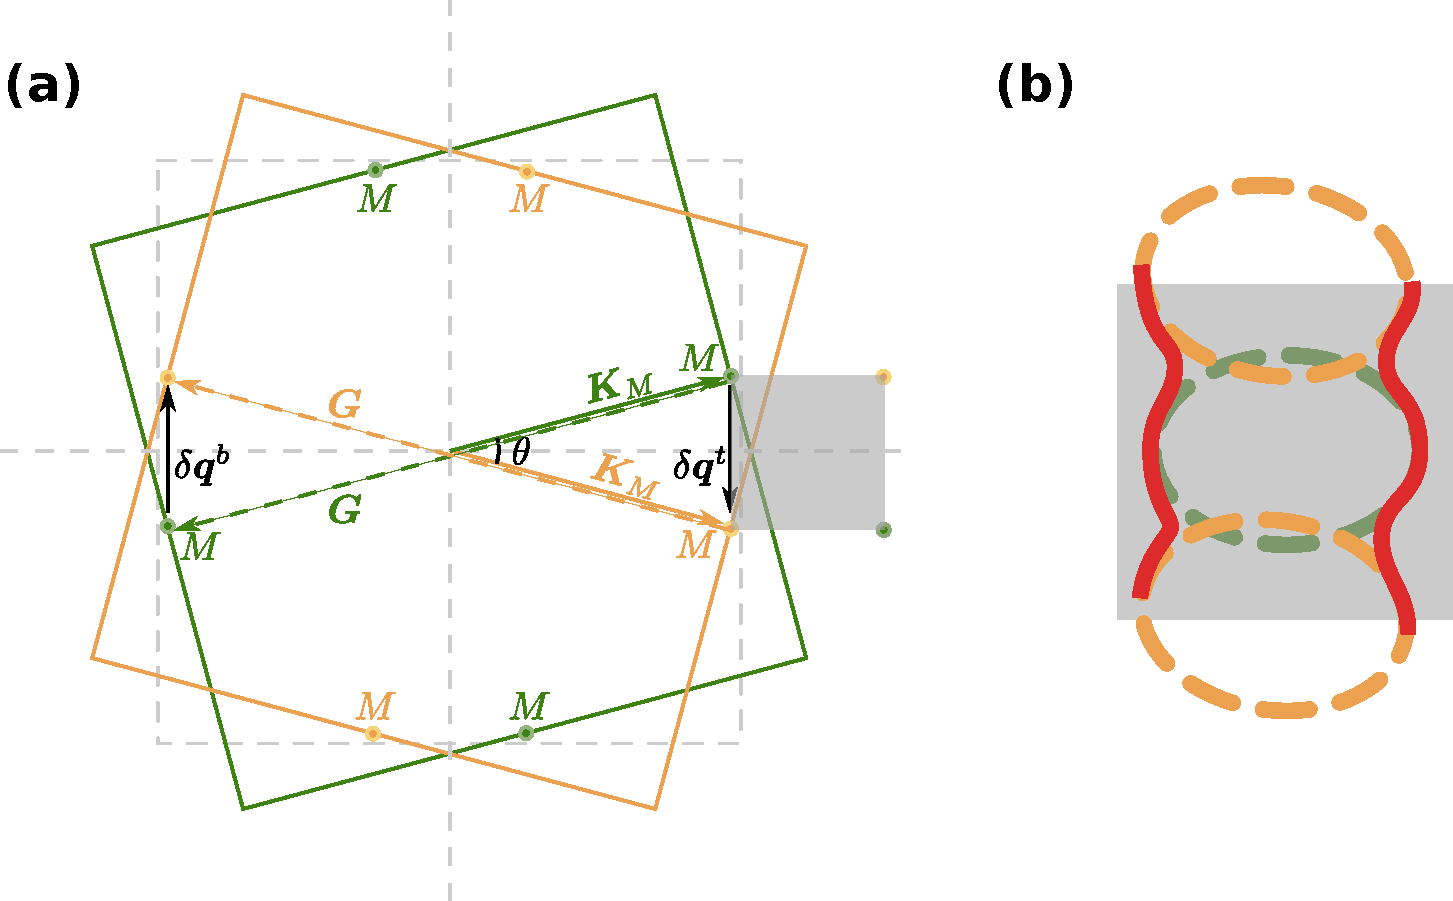
\includegraphics[width=0.85\textwidth]{contents/SATHE/figures/rotated_M-pocket.pdf}
	\caption{(a) Rotated top layer (green) and bottom layer (orange). The interference of all different hopping processes capture the spatial variation of interlayer tunnelings, which determines the moir\'{e} Brillouin zone (gray square). Up to the lowest truncation on such moir\'{e} k-shell, there are just two vertical hopping vectors $\delta\bm{q}^t$ and $\delta\bm{q}^b$ involved in the reconstruction of the left/right $M$-pockets (ditto for the top/bottom ones under a $C_4$-rotation). (b) Illustration for the moire-pattern-involved Fermi surface reconstruction. Taking the top layer elliptic Fermi surface (green dashed lines) as the reference, both the rotated bottom layer (down orange dashed lines) and the copied $M$-pockets due to $G_x$ (up orange dashed lines) involve in the reconstruction of the Fermi surfaces (red solid lines).}
	\label{fig:M-pocket Moire}
\end{figure}
Denoting $t(|\bm{K}_M|)/V\equiv w$, such truncation gives rise to the minimal moir\'{e} Hamiltonian
\begin{equation}\label{moire Hamiltoinian}
	H^{\text{moir\'{e}}}(\bm{k})=\left(\begin{array}{ccc}
		h_{\theta/2}(\bm{k}) & w & w \\
		w & h_{-\theta/2}(\bm{k}+\delta\bm{q}^t) & 0 \\
		w & 0 & h_{-\theta/2}(\bm{k}+\delta\bm{q}^b)
	\end{array}\right).
\end{equation}
The moir\'{e} pattern-induced Fermi surface reconstruction is then obtained by diagonalization Eq.\eqref{moire Hamiltoinian}, which recovers the two vertical \emph{open} curves in (a1) of Fig.2 in the main text. The other two horizontal curves comes from the interference of the hopping processes between the up/down $M$-pockets.

\end{subappendices}
% \chapter{Projective Construction of Composite Fermion States in Fractional Chern Insulators}

\newcommand{\llangle}{\langle\!\langle}
\newcommand{\rrangle}{\rangle\!\rangle}


\section{Introduction}
Fractional Chern insulators (FCI) were theoretically proposed about a decade ago \cite{neupert2011fractional,tang2011high,sheng2011fractional,sun2011nearly,regnault2011fractional,xiao2011interface} as fractional quantum Hall states in the absence of the external magnetic field. Different from the traditional fractional quantum Hall (FQH) states realized in Landau Levels (LL), in FCI the electrons partially fill a nearly flat Chern band, and the Berry's curvature from the Chern band plays the role of the magnetic field. When Coulomb interactions are strong enough compared with the bandwidth of the Chern band, fractional quantum Hall states may be realized, which may host Abelian or non-Abelian anyon excitations. Although the theoretical possibility of such fascinating correlated states of matter in realistic materials has been known for quite some time, and intensive experimental efforts have been made in various candidate materials \cite{xie2021fractional}, only recently the experimental signatures of FCI have been reported in twisted MoTe$_2$ bilayer systems \cite{cai2023signatures,zeng2023thermodynamic,park2023observation,xu2023observation} and rhombohedral pentalayer graphene/hBN moiré superlattice \cite{lu2024fractional}.

In traditional FQH states, the energy scale of the excitations is determined by the Coulomb energy scale $\frac{e^2}{\epsilon l_B}$, where $l_B$ is the magnetic length and $\epsilon$ is the dielectric constant. In FCI, however, $l_B$ should be essentially replaced by the lattice constant $a$ of the crystalline order. This suggests that FCI states, as a matter of principle, may host dynamics with much larger energy scales, and could be ideal experimental platforms to investigate quantum phenomena like anyon statistics. The ongoing theoretical development mainly focus on clarifying the criterion to realize FCI phases, from ideal flatband condition to vortexability \cite{roy2014band,wang2021exact,wang2023origin,estienne2023ideal,ledwith2023vortexability}, and on constructing analytic ground state wavefunctions in certain limits \cite{ledwith2020fractional,dong2023many,wang2023origin}. However, the microscopic theoretical tools suitable to study FCI states are limited: the main theoretical tools currently available include exact diagonalization (ED) and density matrix renormalization group (DMRG) numerics \cite{haldane1985finite,feiguin2008density,dong2023anomalous,dong2023composite,yu2023fractional,goldman2023zero,dong2023theory}. Several outstanding issues are directly related to the ongoing experimental efforts, yet they are challenging to answer using the available theoretical tools. Below, we remark on some of them.

Some of these issues concern the ground state properties of FCI systems. One crucial question is whether the experimental FCI states realize entirely new states of matter, that are not adiabatically connected to the traditional LL FQH states. Theoretically, from the classification viewpoint, such new states of matter could exist from two perspectives. First, the topological order, namely the anyon contents of the FCI states may not be realized in traditional FQH states. Second, even if the topological orders of the FCI states is identical to the traditional FQH states, the presence of the crystalline symmetry may enrich the topological orders, giving rise to different symmetry-enriched topological (SET) states \cite{mesaros2013classification,lu2016classification}. One such SET phenomenon that has been discussed in the literature is the analog of the Wen-Zee shift \cite{wen1992shift} for the discrete crystalline rotation symmetry group \cite{manjunath2023rotational,han2019generalized,li2020fractional,zhang2022fractional}, which is related to the spin angular momentum carried per quasiparticle. Nontrivial Wen-Zee shift would lead to, for instance, fractionally quantized charges at lattice disclinations in the bulk \cite{li2020fractional,zhang2022fractional}.

In the traditional FQH context, the composite fermion states \cite{jain1989composite} are associated with a simple mean-field picture. After the flux attachment \cite{jain1990theory}, the electron in a physical LL becomes a composite fermion (CF) that sees an effective magnetic field -- a fraction of the physical magnetic field. Consequently, the CF fills an integer number of effective composite fermion LLs. The Jain's sequence at filling $\nu=\frac{p}{2ps+1}$ corresponds to attaching $2s$-unit of flux to the electron, and the CF fills $p$ CF LLs. Note that the CF wavefunction is a free fermion state in this mean-field picture -- a Slater determinant. The physical electronic wavefunction, e.g., the Laughlin's wavefunctions, obviously, is not a Slater determinant.

In the FCI context, this mean-field picture is expected to be modified naturally: the electron LL is replaced by a Chern band, while the CF Chern bands also replace the CF LLs. Physically, the different CF LLs are characterized by the spin angular momentum carried per CF: for the $n$-th ($n=0,1,2...$) CF LL, the CF carries spin angular momentum $l=n$. Although continuous rotation symmetry is absent in the FCI context, the angular momentum mod $m$ is still sharply defined for  $C_m$ crystalline rotation symmetry.

% [Illustration figure of CF LL's.]
\begin{figure}[!htp]
    \centering
    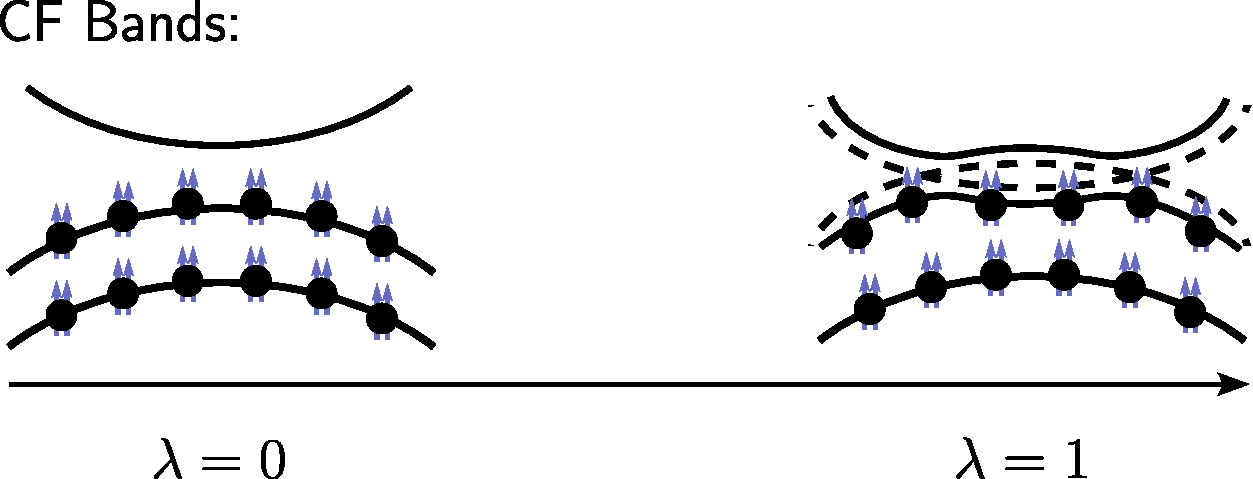
\includegraphics[width=0.45\textwidth]{figures/FCI/CF_band_Wen-Zee_shift_transition.pdf}
    \caption{Illustration for the possible change of Wen-Zee shift due to the CF band inversion when tunning the parameter $\lambda$, so that the CF states at $\lambda=0$ and $\lambda=1$ belongs to different SET phases.}
    \label{fig:CF band inversion}
\end{figure}

As a thought experiment, one may imagine smoothly deforming the electronic Hamiltonian $H(\lambda)$ with a parameter $\lambda$ while preserving the physical symmetries so that a LL CF state at $\lambda=0$ is connected with an FCI CF state at $\lambda=1$. The question is whether or not the two states are in the same quantum phase.  The physics of topological insulators teaches us that band inversion may give rise to new states of matter. Indeed, when the CF Chern bands have a full band inversion from $\lambda=0$ to $\lambda=1$, the system would have a corresponding change of the Wen-Zee shift, in which case the two states are in different SET phases. See FIG.\ref{fig:CF band inversion} for illustration.


Some other theoretical issues are about the dynamical properties of the FCI states. For instance, the magnetorotons are the charge-neutral bulk excitations and have been experimentally probed using Raman scattering in the traditional FQH systems \cite{pinczuk1998light,kang2000inelastic,kukushkin2009dispersion}. In the presence of the Galilean invariance, the magnetoroton at wavevector $q=0$ has been recently interpreted by Haldane as the collective mode of the geometry fluctuations \cite{haldane2011geometrical,haldane2009hall}, analogous to the graviton, carrying angular momentum $l=\pm 2$ \cite{yang2012model}.  In the FCI systems, there is no reason these magnetorotons necessarily carry angular momentum  $l=\pm 2$. What are the crystalline quantum numbers carried by the magnetorotons in FCI systems? How to theoretically compute the magnetoroton spectra in FCI systems? These questions are also relevant to the quantum phase transitions involving FCI states. For instance, when magnetorotons become gapless at certain momenta, the system is expected to break translational symmetry and develop charge density wave order.

Due to the limitation of the small system sizes for ED and the difficulty of implementing DMRG on sizable torus samples, answering questions about the crystalline quantum numbers has been challenging for FCI systems. Developing new theoretical tools to investigate these important questions would be desirable.

On the other hand, a different class of quantum systems hosting topologically ordered phases is the quantum spin liquids. There, a nice theoretical tool is available: projective constructions such as the Schwinger-boson and Abrikosov-fermion methods \cite{arovas1988functional,read1991large,sachdev1991large,sachdev1992kagome,wang2010schwinger,wen1991mean,wen2002quantum,gros1989physics,tay2011variational}. These projective constructions are very helpful: they provide mean-field theories for the topologically ordered states by enlarging the physical Hilbert space. The mean-field wavefunctions can be improved by projection back to the physical space, leading to physical wavefunctions that can be directly compared with other numerical methods, e.g., ED and DMRG. The detailed microscopic information, such as the crystalline symmetry quantum numbers carried by the ground states and excited states, is accessible in these methods. However, in FCI systems, similar projective construction has been lacking.

Motivated by these issues, we establish a projective construction for the composite fermion states in fractional Chern insulators in this paper. Our main results can be summarized as a general procedure. The procedure input is the Hamiltonian $\mathbf H_{\text{CB}}$ describing a partially filled Chern band with Chern number $C=\pm 1$, which we want to investigate. The procedure output is two-fold. First, on the mean-field level, the procedure outputs a Hartree-Fock (HF) mean-field Hamiltonian for the CF states in an enlarged Hilbert space, whose ground state is the CF wavefunction $|\psi^{MF}_{CF}\rangle$ and is a Slater determinant. The excitations of the system (e.g., the magnetoroton collective modes) can be calculated within the time-dependent Hartree-Fock (TDHF) framework. Second, beyond the mean-field level, the CF wavefunction can be projected into the physical electronic wavefunction $|\psi_{e}(\psi^{MF}_{CF})\rangle=\mathbf P |\psi^{MF}_{CF}\rangle$ ($\mathbf P$ is a projector), which turns out to be a so-called hyperdeterminant of a tensor and can be compared with wavefunctions obtained from ED.

The paper is organized as follows. Because we will discuss both $|\psi^{MF}_{CF}\rangle$ and $|\psi_{e}(\psi^{MF}_{CF})\rangle$, to avoid confusion, below we will denote the former wavefunction as the mean-field (MF) CF state, while the latter wavefunction as the electronic (or projected) CF state.  To present a self-contained discussion, in Sec.\ref{sec:review} we briefly review several related pieces of previous works, including Jain's CF construction \cite{jain1990theory}, Murthy-Shankar's Hamiltonian formalism \cite{murthy2003hamiltonian}, the construction of $\nu=1$ bosonic composite Fermi liquid developed by Pasquier-Haldane \cite{pasquier1998dipole} and Read \cite{read1998lowest}. In Sec.\ref{sec:M_S_finite} we discuss the general projective construction on finite-size crystalline systems for composite fermion states (either in the Jain's sequence or the composite Fermi liquid), which is based on Murthy-Shankar's construction.  This projective construction leads to the MF CF ground states and excited states on the mean-field level, as well as a projection operation $\mathbf P$ to go beyond the mean-field. In Sec.\ref{sec:proj}, we study the mathematical details of the projection $\mathbf P$ operation and show that the general projected CF states are hyperdeterminants of tensors. We then connect our results with previous works including Jain's construction in the traditional FQH context and the parton construction in the FCI context. Interestingly, despite the current construction reproduces Jain's wavefunctions in the traditional Galilean invariant Landau level context, in the absence of the Galilean invariance (e.g. in a FCI system), the present construction and the naive generalization of Jain's prescription are \emph{different} in general. In Sec.\ref{sec:benchmark}, we apply this general procedure to two microscopic FCI models: a toy model of mixed Landau levels introduced by Murthy and Shankar \cite{murthy2012hamiltonian}, and the realistic model for the twisted bilayer MoTe$_2$ \cite{wang2023fractional}. Experimentally relevant properties of the FCI states are computed, such as the magnetoroton quantum numbers and spectra. Finally, we discuss possible future developments of our construction and conclude in Sec.\ref{sec:conclusion}


\section{A brief review of related previous works}\label{sec:review}
\subsection{Jain's composite-fermion construction}
Jain's wavefunctions for composite fermion states \cite{jain1989composite,jain1989incompressible,jain1990theory,jain2007composite,balram2013state} are based on the seminal idea of the flux attachment. To describe the fractional quantum Hall states at filling $\nu=\frac{p}{2ps+1}$ where $p,s\in\mathbb Z$ are integers, Jain proposed the following wavefunctions in the symmetric gauge of the lowest Landau level with the open boundary condition \cite{kamilla1996composite}:
\begin{align}\label{eq1. Jain's wave function}
    \psi_{\frac{p}{2ps+1}}=\mathcal P_{\text{LLL}} \prod_{i<j} (z_i-z_j)^{2s}\cdot \chi_p(z,\bar z)
\end{align}
Here $\chi_p(z,\bar z)$ is the Jain's composite fermion wavefunction with $p$-filled Landau levels. The flux attachment in this scheme is achieved by the Jastrow factor $(z_i-z_j)^{2s}$: when one electron moves around another electron by a circle, this factor gives a $4\pi s$ phase shift, similar to when an electron moves around $2s$-flux tube. The projection operation $\mathcal P_{\text{LLL}}$ ensures the final wavefunction is within the lowest Landau level (LLL). Precisely, Jain proposes the prescription to replace $\bar z$ by the derivative $\mathcal P_{\text{LLL}}: \bar z\rightarrow 2 l_e^2 \frac{\partial}{\partial z}$, where $l_e$ is the electron's magnetic length. By moving all the derivatives to the left, the obtained wavefunction is holomorphic as required by the LLL. Jain's wavefunctions, after adapted to appropriated boundary conditions, have been demonstrated to have excellent overlap with those obtained from the exact diagonalization.

Jain's composite fermion wavefunction $\chi_p(z,\bar z)$ is a single Slater determinant. In the simplest $p=1$ case, it is the Vandermonde determinant together with the Gaussian factor:
\begin{align}
    \chi_{p=1} & =\det\left|\begin{array}{cccc}
                                z_1^0  & z_2^0  & z_3^0  & \cdots \\
                                z_1^1  & z_2^1  & z_3^1  & \cdots \\
                                z_1^2  & z_2^2  & z_3^2  & \cdots \\
                                \vdots & \vdots & \vdots & \ddots
                            \end{array}\right|\exp\left[-\sum_{i}\frac{|z_i|^2}{4l_e^2}\right]\notag                         \\
               & =\prod_{i<j}(z_i-z_j)~\exp\left[-\sum_{i}\frac{|z_i|^2}{4l_e^2}\right].\label{eq.2 Jain's CF wave function}
\end{align}
In this particular case, the projection $\mathcal P_{\text{LLL}}$ is unnecessary since $\bar z$ is not present, and Jain's wavefunctions becomes Laughlin's wavefunctions \cite{laughlin1983anomalous}.

Despite the success of Jain's wavefunctions in the FQHE, how to generalize them to the context of FCI remains unclear. In fact, we want to mention two conceptual puzzles in Jain's original construction, which motivated us to develop the new construction. First, the physical meaning of the composite fermion Landau levels needs to be clarified. For instance, how many composite fermion Landau levels are there? In a finite-size system, the dimension of the physical electronic Hilbert space is finite. It would be unphysical to have a construction involving an infinite number of composite fermion Landau levels. So, if this number is finite for a finite-size sample, what is it?

Second, let us pay attention to the Gaussian factor $\exp\left[-\sum_{i}\frac{|z_i|^2}{4l_e^2}\right]$ in the composite fermion state Eq.\eqref{eq.2 Jain's CF wave function}. The puzzle is the appearance of the \emph{electronic} magnetic length $l_e$. On the one hand, this is required by Jain's prescription to obtain a wavefunction $\psi_{\frac{p}{2ps+1}}$ within the LLL of the electrons. On the other hand, physically, if the composite fermion sees a weaker magnetic field with an effective magnetic length $l_{CF}>l_e$, wouldn't $l_{CF}$ be appearing in the Gaussian?

We will come back to these two puzzles in Sec.\ref{sec:connection_jain}, where we demonstrate that the new construction solves both puzzles naturally.

\subsection{Murthy-Shankar's Hamiltonian theory}
Focusing on the composite fermion states, Murthy and Shankar developed a Hamiltonian theory for FQHE \cite{murthy2003hamiltonian}. Let us first set up some basic notations. The electron's full position operator $\bm r_e$ can be separated into the mutually commuting guiding-center $\mathcal R_e$ and cyclotron $\eta_e$ degrees of freedom:
\begin{align}
    \bm r_e=\mathcal R_e+\eta_e,
\end{align}
satisfying the algebra:
\begin{align}\label{eq:e_guiding_center}
    [\mathcal R_{e,x},\mathcal R_{e,y}]=-il_e^2, \quad [\eta_{e,x},\eta_{e,y}] & =il_e^2
\end{align}

For the dynamics within the LLL, the $\eta_e$ degrees of freedom are frozen and one needs to focus on the guiding-center part of the density operator ($i$ labels the particle)
\begin{align}
    \pmb{\boldsymbol\rho}_e(\mathbf q_e)=\sum_{i}e^{i\mathbf q_e\cdot \mathcal R_{e(i)}},\label{eq:e_density}
\end{align}
which satisfies the Girvin-MacDonald-Platzman (GMP) algebra \cite{girvin1986magneto}
\begin{align}
    [\pmb{\boldsymbol\rho}_e(\mathbf q_e),\pmb{\boldsymbol\rho}_e(\mathbf q_e')] & =2i\sin\left[\frac{\mathbf q_e\times \mathbf q_e'}{2}l_e^2\right]\pmb{\boldsymbol\rho}_e(\mathbf q_e+\mathbf q_e')\label{eq:GMP}
\end{align}
The electron Hamiltonian constrained within the LLL can be represented using this density operator. For instance, for the Coulomb interaction,
\begin{align}
    \mathbf H_e=\frac{1}{2 A}\sum_{\mathbf q_e} e^{-\frac{\mathbf q_e^2l_e^2}{2}}v(\mathbf q_e):\pmb{\boldsymbol\rho}_e(\mathbf q_e)\pmb{\boldsymbol\rho}_e(-\mathbf q_e):,
\end{align}
where $v(\mathbf q_e)=\frac{2\pi e^2}{\epsilon |\mathbf q_e|}$ and $A$ is the real-space sample size.

To achieve the flux attachment, Murthy and Shankar introduced auxiliary degrees of freedom, the vortex guiding-center $\mathcal R_v$, to enlarge the Hilbert space:
\begin{align}
    [\mathcal R_{v,x},\mathcal R_{v,y}] & =il_v^2.\label{eq:v_guiding_center}
\end{align}
Here the vortex magnetic length $l_v=\frac{l_e}{c}$ with $c=\sqrt{\frac{2ps}{2ps+1}}$. Physically, $\mathcal R_v$ describes the vortex that carries an electric charge $q_v$ that has an opposite sign of the electron's electric charge $q_e$:  $q_v=-\frac{2ps}{2ps+1}q_e$. With these auxiliary degrees of freedom, the full composite fermion degrees of freedom can be constructed, including the mutually commuting guiding-center and the cyclotron components:
\begin{align}
    \mathcal R_{CF}=\frac{\mathcal R_e-c^2\mathcal R_v}{1-c^2}, \quad \eta_{CF}=\frac{c}{1-c^2}(\mathcal R_v-\mathcal R_e), \label{eq:CF_substitution}
\end{align}
satisfying the algebra:
\begin{align}
    [\mathcal R_{CF,x},\mathcal R_{CF,y}]=-il_{CF}^2, \quad [\eta_{CF,x},\eta_{CF,y}]=il_{CF}^2.\label{eq:CF_algebra}
\end{align}
Here the CF magnetic length $l_{CF}=\frac{l_e}{\sqrt{1-c^2}}=\sqrt{2ps+1}l_e$, which can be interpreted as the CF electric charge $q_{CF}=\frac{q_e}{2ps+1}$. We also list the inverse transformation of Eq.(\ref{eq:CF_substitution}):
\begin{align}
    \mathcal R_e=\mathcal R_{CF}+c\cdot\eta_{CF}, \quad \mathcal R_v=\mathcal R_{CF}+\frac{1}{c}\eta_{CF}\label{eq:CF_substitution_inverse}
\end{align}

If we denote the electron's and the vortex's single-particle Hilbert spaces as $\mathcal H_e$ and $\mathcal H_v$,  the composite fermion lives in an enlarged Hilbert space $\mathcal H_{CF}=\mathcal H_e\otimes \mathcal H_v$, that can be decomposed into CF's guiding-center and the cyclotron components: $\mathcal H_{CF}=\mathcal H_{\mathcal R_{CF}}\otimes \mathcal H_{\eta_{CF}}$.

Any physical operator $\hat O_e$ acting in the electronic Fock space, including the Hamiltonian $\mathbf H_e$, then can be mapped to the composite fermion Fock space. As a fundamental example, the electron's density operator can be identified with:
\begin{align}
    \pmb{\boldsymbol\rho}_e(\mathbf q_e)=\sum_{i}e^{i\mathbf q_e\cdot \mathcal R_{e(i)}} \rightarrow \sum_{i}e^{i\mathbf q_e\cdot\left[\mathcal R_{CF(i)}+c\cdot\eta_{CF(i)}\right]}  \label{eq:rho_CF_substitution}
\end{align}
The composite fermion states with $p$-filled CF LLs can be viewed as the Hartree-Fock mean-field ground states of $\mathbf H_e$. In addition, the bulk excitations such as the magnetorotons spectra can be computed within the time-dependent Hartree-Fock framework \cite{murthy1999hamiltonian, murthy2001hamiltonian}. These mean-field results are qualitatively consistent with other calculation methods.

More recently, Murthy and Shankar generalized this Hamiltonian approach to the context of FCI \cite{murthy2012hamiltonian}. This generalization is based on two important observations. First, the bloch states in a Chern band with Chern number $C=\pm 1$ can be mapped to the wavefunctions in the LLL on a torus \cite{haldane1985periodic}. Accordingly, an FCI Hamiltonian with $C=\pm 1$ can be exactly mapped to an electronic Hamiltonian in the LLL, with the presence of a crystalline potential. Second, the density operators as $\rho_e(\mathbf q_e)$ in Eq.(\ref{eq:e_density}) on a finite-size torus actually form a complete basis for any fermion bilinears (i.e., single-body operators). Therefore, any density-density interactions can also be straightforwardly mapped into the LLL problem based on Eq.(\ref{eq:rho_CF_substitution}).

In Murthy-Shankar's Hamiltonian construction, the physical origin of the CF LL is clear as it is a consequence of the enlarged Hilbert space. The relation with Jain's wavefunctions, however, remains a puzzle. It is also unclear how to improve beyond the mean-field treatment, a challenge related to the gauge structure of the construction that was first studied by Read \cite{read1998lowest} in the context of the bosonic $\nu=1$ composite Fermi liquid, as we will discuss shortly.

\subsection{Pasquier-Haldane-Read construction for the bosonic $\nu=1$ composite fermion liquid}
The Pasquier-Haldane's work \cite{pasquier1998dipole} considered bosonic charged particles at $\nu=1$. Here, one may argue that after attaching one unit flux, the boson becomes a composite fermion that sees no effective magnetic field, which forms a composite Fermi sea. The boson's Fock space is enlarged by introducing fermions with two indices $c_{mn}$ satisfying the usual algebra:
\begin{align}
    \{c_{mn},c^\dagger_{m'n'}\}=\delta_{mm'}\delta_{nn'}.
\end{align}
Here $m,n\in 1,2,...N$, and $N$ is the number of bosonic particles and the number of orbitals in the LLL. The basis states of the physical Fock space of bosons are then constructed as
\begin{align}
    |m_1,m_2,...,m_N\rangle=\epsilon^{n_1,n_2,...,n_N} c_{n_1m_1}^\dagger c_{n_2m_2}^\dagger ... c_{n_N m_N}^\dagger|0\rangle,\label{eq:Read_projection}
\end{align}
where $|0\rangle$ is the vacuum of the $c_{mn}$ fermion's Fock space, and $\epsilon$ is the fully antisymmetric Levi-Civita symbol, and we have used the Einstein notation. Read \cite{read1998lowest} studied the mean-field theory and gauge fluctuations of this theory. As any theory involving an enlarged Hilbert space, the physical state is obtained only when the gauge redundancy is removed. In the present case, the constraint that the physical states need to satisfy is exactly the invariance under the $SU(N)_R$ transformation generated by (apart from the trace):
\begin{align}
    \pmb{\boldsymbol\rho}^R_{nn'}=c^\dagger_{nm} c_{mn'}
\end{align}
On the other hand, the physical density operators are:
\begin{align}
    \pmb{\boldsymbol\rho}^L_{mm'}=c^\dagger_{nm'} c_{mn}
\end{align}
Note that $\pmb{\boldsymbol\rho}_R$ and $\pmb{\boldsymbol\rho}_L$ commute. The constraint can then be implemented as the identity on the operator level: $\pmb{\boldsymbol\rho}^R_{nn'}=\delta_{nn'}$, which is treated using the Hartree-Fock and time-dependent Hartree-Fock approximation (also called the conserving approximation) in Ref.\cite{read1998lowest}.

The Pasquier-Haldane-Read construction, although only applicable to the bosonic $\nu=1$ CFL, is closely related to the Murthy-Shankar Hamiltonian theory, which we will explain below.

\section{The projective construction on a finite-size system}\label{sec:M_S_finite}
In this section, step by step, we present a general projective construction of CF states applicable for both traditional FQHE and FCI systems. Several steps of this construction are based on Murthy-Shankar's Hamiltonian theory but on finite-size systems.

\emph{In this paper, to avoid confusion, we will always use the regular font for operators in the single-particle Hilbert spaces and the bold font for corresponding operators in many-particle Fock spaces.}

\subsection{Mapping a Chern band to the lowest Landau level}
Soon after the theoretical proposal of the FCI, it is understood that a generic Chern band with Chern number $C=\pm1$ can be mapped to the LLL preserving the crystalline symmetries\cite{qi2011generic,wu2013bloch, jian2013crystal}. Recently, further investigations have been made on various ideal Chern band conditions which could allow exact mapping of ground state wavefunctions between FCI systems and FQH systems, in the presence of certain short-range interactions\cite{roy2014band,wang2021exact,wang2023origin,estienne2023ideal,ledwith2020fractional,ledwith2023vortexability,dong2023many}. However, in the present work, we are motivated to investigate generic FCI states which potentially are far away from the FQH systems. Therefore, we will focus on the generic Chern band mapping\cite{qi2011generic,wu2013bloch, jian2013crystal} without invoking ideal band conditions.

In this section, we present a detailed construction for such a mapping. The main results are summarized as follows. We construct the bloch basis in the LLL in Eq.(\ref{eq:bloch_condition},\ref{eq:rho_matrix_element}), represented using the Jabobi's $\vartheta$-function introduced by Haldane and Rezayi\cite{haldane1985periodic} as illustrated in Fig.\ref{fig:LLL_bloch_basis}. A Hamiltonian in a generic Chern band $\mathbf H_{CB}$ can then be exactly mapped to a Hamiltonian in the LLL $\mathbf H_{e}$ following the Hilbert space mapping in Eq.(\ref{eq:CB_LLL_map}). The crystalline translation/rotation symmetries in $\mathbf H_{CB}$ are mapped into the magnetic translation/rotation symmetries in $\mathbf H_{e}$ in Eq.(\ref{eq:CB_map_LLL_symmetry}). Note that since the Hamiltonian $\mathbf H_{e}$ in the LLL faithfully contains all the lattice-scale physics of $\mathbf H_{CB}$, $\mathbf H_{e}$ generally does not have Galilean invariance as in the traditional FQH problems. Finally, for the purpose of performing practical calculations, it is convenient to represent $\mathbf H_{e}$ using the electron density operators in the LLL as shown in Eq.(\ref{eq:H_e}).

Firstly, let us introduce the single-particle bloch basis in the LLL. The mutually commuting guiding-center and cyclotron degrees of freedom in the LLL are ($e>0$):
\begin{align}
    \mathcal R_e=\bm r_e-\eta_e, \quad \eta_e=\frac{l_e^2}{\hbar}\hat z\times (\mathbf p_e+e\mathbf A_e),
\end{align}
where the magnetic length $l_e\equiv \sqrt{\frac{\hbar}{eB_e}}$. The usual kinetic Hamiltonian only depends on the $\eta_e$:
\begin{align}
    H_K= \frac{(\mathbf p_e+e\mathbf A_e)^2}{2m_e}=\frac{\hbar^2}{2m_e l_e^4}\eta_e^2.
\end{align}
Without loss of generality, we choose the Landau gauge $\mathbf A_e=(B_e y,0)$ in this section. The subscript $e$ highlights the objects for physical electrons, because, in the next step, we will introduce similar objects for vortices and composite fermions.

\emph{Throughout this paper, unless explicitly stated otherwise, we focus on the case with $B_e>0$, whose LLL has a Chern number $C=-1$.} For Chern band systems whose Chern number $C=+1$, one needs to perform a time-reversal transformation to map to the LLL discussed here.

\emph{To save notation, we will interchangeably use the complex number $z\equiv x+iy$ to represent a vector $\bm r\equiv(x,y)$}. The single-particle magnetic translation operator is
\begin{align}
    D_e(z_0)\equiv U_{T,e}(z_0)T_e(z_0),
\end{align}
where $T_e(z_0)$ is the usual translation operator: $T_e(z_0)\psi_e(z)=\psi_e(z-z_0)$, and $U_{T,e}(z_0)$ is the associated gauge transformation that is fixed up to a $U(1)$ phase factor. One choice to fix this $U(1)$ phase ambiguity is to define $D_e(z_0)$ as the density operator:
\begin{align}
    D_e(z_0)\equiv\rho_e(\mathbf q_{e, z_0})=e^{i \mathbf q_{e, z_0} \cdot \mathcal R_e}, \quad\text{where }\mathbf q_{e, z_0}\equiv i\frac{z_0}{l_e^2}.\label{eq:real_momentum}
\end{align}

We will fix this definition in the discussion below. One may straightforwardly check that the explicit form of $U_{T,e}(z_0)$ is now
\begin{align}
    U_{T,e}(z_0)=e^{\frac{i}{2l_e^2}(x_0y_0-2y_0 x)}\label{eq:U_T}
\end{align}
The magnetic translations satisfy the algebra:
\begin{align}
    D_e(z_0)D_e(z_1) & =e^{\frac{i}{2l_e^2}(x_0 y_1-y_0 x_1)}D_e(z_0+z_1),
\end{align}
and consequently, they satisfy the commutation relation
\begin{align}
    [D_e(z_0),D_e(z_1)]=2i\sin\frac{x_0 y_1-y_0 x_1}{2l_e^2} D_e(z_0+z_1).
\end{align}
This is just another way to write down the GMP algebra Eq.(\ref{eq:GMP}).

Note that, although on the single-particle level we have Eq.(\ref{eq:real_momentum}),  the many-particle versions of the density operator and the magnetic translation operator in the Fock spaces are defined differently. In the first-quantization language:
\begin{align}
    \pmb{\boldsymbol\rho}_e(\mathbf q_e) & \equiv \sum_i \rho_e(\mathbf q_e)_{(i)}\notag \\
    \pmb{\bm D}_e(z_0)                   & \equiv \prod_i D_e(z_0)_{(i)},
\end{align}
where the subscript-$i$ means the operator is acting on the $i$-th particle. They satisfy:
\begin{align}
    \pmb{\bm D}_e(z_0)\pmb{\boldsymbol\rho}_e(\mathbf q_e)\pmb{\bm D}_e(z_0)^\dagger=e^{i\mathbf q_e\cdot z_0}\pmb{\boldsymbol\rho}_e(\mathbf q_e)\label{eq:D_e_rho_e}
\end{align}
We will come back to these many-particle operators later.

On a finite-size torus, the boundary conditions can be described by the operator identities:
\begin{align}
    D_e(L_1)=e^{-i\varphi_{e,1}}, \quad D_e(L_1\tau)=e^{-i\varphi_{e,2}},\label{eq:boundary_conditions}
\end{align}
where $L_1>0$, $\tau$ is a complex number with positive imaginary part capturing the shape of the sample, and $L_1$ and $|L_1\tau|$ specify the real-space sample size. Note that $D_e(L_1)$ and $D_e(L_1\tau)$ must commute to apply the boundary conditions, leading to the flux quantization condition: the total number of fluxes through the sample is an integer $N_{\phi,e}$.

Haldane and Rezayi \cite{haldane1985periodic} pointed out that the orbital wavefunctions in the LLL, in the present gauge, can be compactly written in terms of the odd Jacobi-$\vartheta$ function, parameterized by $N_{\phi,e}$ zeros $z_\nu$ ($\nu=1,2,...,N_{\phi,e}$) and a complex number $k$ (Note that the convention for the magnetic translation in the present work differs from that in Ref.\cite{haldane1985periodic} by a minus sign.):
\begin{align}
    \psi_e(z) & \propto f(z)e^{-\frac{y^2}{2l_e^2}},\notag                                                                         \\
              & \text{ with } f(z)=e^{ikz}\prod_{\nu=1}^{N_{\phi,e}}\vartheta_1(\pi(z-z_\nu)/L_1 | \tau), \label{eq:Haldane_theta}
\end{align}
where the value of $k$ and the sum of zeros $z_{sum}\equiv\sum_{\nu} z_\nu$ need to be consistent with the boundary conditions:
\begin{align}
    e^{ikL_1}               & =(-1)^{N_{\phi,e}}\cdot e^{i\varphi_{e,1}},\notag                       \\
    e^{i 2\pi z_{sum}/L_1 } & =(-1)^{N_{\phi,e}}\cdot e^{i\varphi_{e,2}-ikL_1\tau}. \label{eq:k_z_nu}
\end{align}
Although it appears that the wavefunction can be smoothly tuned, there are only $N_{\phi,e}$ linearly independent wavefunctions. Let $(k_0,z_{sum,0})$ be one solution of Eq.(\ref{eq:k_z_nu}),
the other solutions have the form:
\begin{align}
    k=k_0+\frac{2\pi l_1}{L_1},\quad z_{sum}=z_{sum,0}+l_2 L_1-l_1 L_1\tau, \quad l_i\in\mathbb Z \label{eq:diff_z_sum}
\end{align}

In order to study a Chern-band sample with $N_{1,e}\cdot N_{2,e}$ unit cells, one can construct the corresponding bloch basis in the LLL. Namely, we consider the two real-space basis vectors $\mathbf a_{1,e},\mathbf a_{2,e}$ with $L_1=N_1 \mathbf a_{1,e}$, and $L_1\tau=N_2 \mathbf a_{2,e}$. $D_e(\mathbf a_{1,e})$ and $D_e(\mathbf a_{2,e})$ need to commute as the usual lattice translations. To have a one-to-one mapping between the Chern band and the LLL, one further chooses the area spanned by $\mathbf a_{1,e},\mathbf a_{2,e}$ contains exactly one flux unit, so that $N_{1,e}\cdot N_{2,e}=N_{\phi,e}$. With this setup, the minimal magnetic translations along $\mathbf a_{1,e},\mathbf a_{2,e}$ directions allowed by the boundary conditions are $\frac{\mathbf a_{1,e}}{N_{2,e}},\frac{\mathbf a_{2,e}}{N_{1,e}}$, respectively.

The bloch basis in the LLL is formed by $N_{1,e}\cdot N_{2,e}$ simultaneous eigenstates of $\mathbf a_{1,e},\mathbf a_{2,e}$ magnetic translations:
\begin{align}
    D_e(\mathbf a_{1,e})|\mathbf k_e\rangle_{\text{LLL}} & =e^{-i\mathbf k_e\cdot \mathbf a_{1,e}}|\mathbf k_e\rangle_{\text{LLL}},\notag                     \\
    D_e(\mathbf a_{2,e})|\mathbf k_e\rangle_{\text{LLL}} & =e^{-i\mathbf k_e\cdot \mathbf a_{2,e}}|\mathbf k_e\rangle_{\text{LLL}},\label{eq:bloch_condition}
\end{align}
where
\begin{align}
     & \mathbf k_{e,(m_{1,e},m_{2,e})}\equiv \frac{m_{1,e}+\varphi_{1,e}/(2\pi)}{N_{1,e}} \mathbf G_{1,e} + \frac{m_{2,e}+\varphi_{2,e}/(2\pi)}{N_{2,e}} \mathbf G_{2,e},\label{eq:k_e_vals} \\
     & \mathbf G_{1,e}=\frac{-i\mathbf a_{2,e}}{l_e^2}, \;\;\mathbf G_{2,e}=\frac{i\mathbf a_{1,e}}{l_e^2}.\notag
\end{align}
Here, $\mathbf G_{i,e}$ are the reciprocal basis vectors of $\mathbf a_{i,e}$, where the complex factor $i$ is used in the last line because the reciprocal vector is expressed in complex coordinates, and one may choose a Brillouin Zone (BZ) with $m_{i,e}\in [0,N_{i,e}-1]$ being integers. These bloch states can be written in terms of infinite sums, as performed in Ref.\cite{jian2013crystal,murthy2012hamiltonian} for the case of a square lattice. Here, instead, we simply represent them using Haldane-Rezayi's Jacobi-$\vartheta$ function via parameters $k$ and $z_\nu$.

To satisfy the eigen-condition Eq.(\ref{eq:bloch_condition}), obviously the zeros $z_\nu$ of $|\mathbf k_e\rangle_{\text{LLL}}$ need to form a $N_{1,e}\cdot N_{2,e}$ grid in the real-space:
\begin{align}
    z_\nu=z_1+n_1 \mathbf a_{1,e}+ n_2 \mathbf a_{2,e},\label{eq:bloch_pattern_of_zeros}
\end{align}
where $n_i \in [0,N_{i,e}-1]$ are integers, and $z_1$ can be completely determined by $z_{sum}$ (see FIG.\ref{fig:LLL_bloch_basis} for an illustration).
\begin{figure}
    \centering
    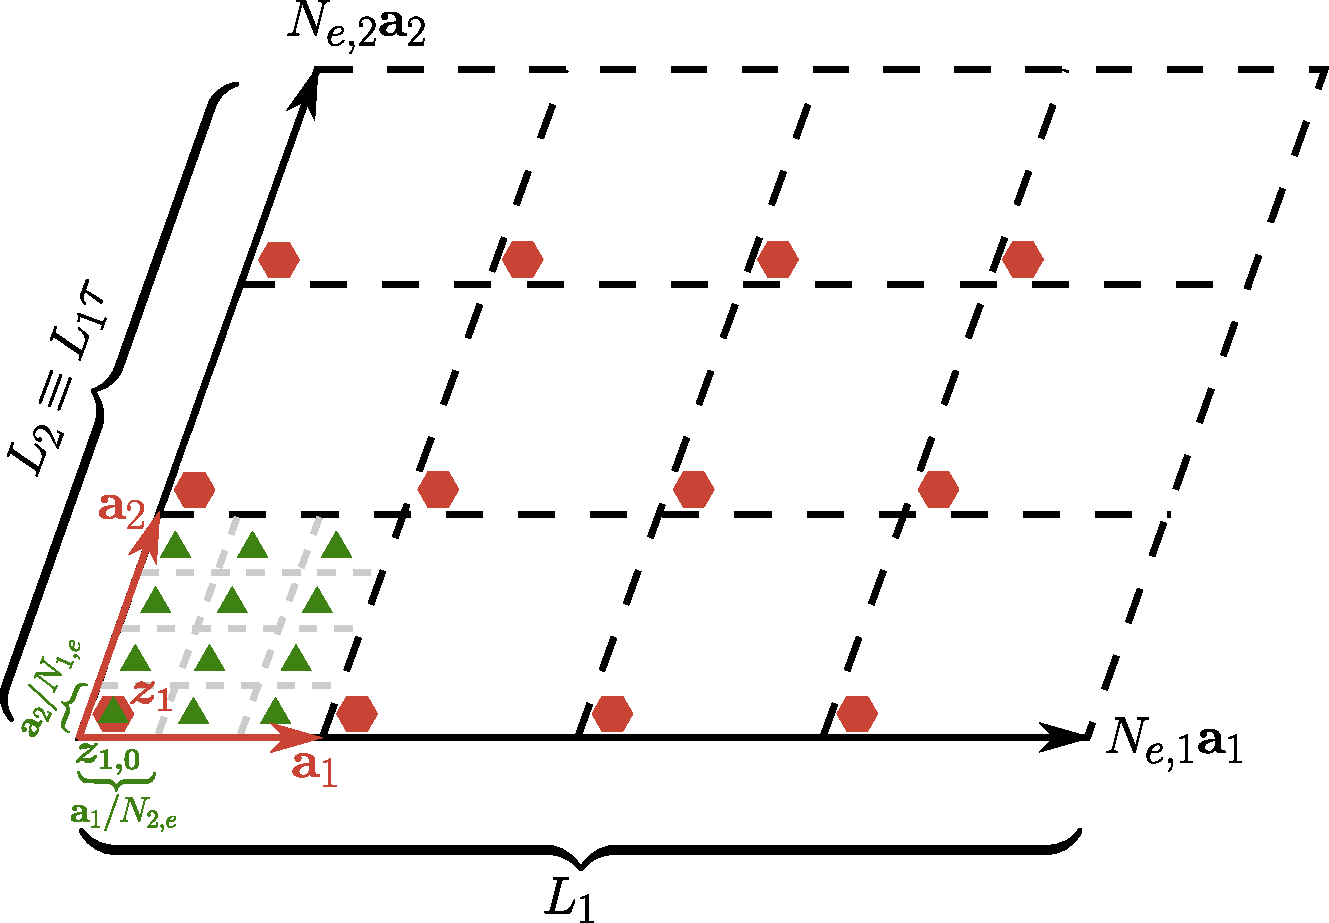
\includegraphics[width=0.75\textwidth]{figures/FCI/Haldane_Rezayi.pdf}
    \caption{Geometry Setup of the LLL Bloch Basis: The torus sample, equivalent to a parallelogram, is parameterized by a real length $L_1$ and a modular parameter $\tau$. The $N_{1,e}\cdot N_{2,e}$ zeros $\{z_\nu\}$ (red hexagons) of the Haldane-Rezayi wave function are equally distributed on the torus sample by construction, see Eq.\eqref{eq:bloch_pattern_of_zeros}. There are also $N_{1,e}\cdot N_{2,e}$ independent groups of $\{k, z_{sum}\}$ satisfying the boundary condition Eq.\eqref{eq:k_z_nu}, i.e. $N_{1,e}\cdot N_{2,e}$ independent basis parameterized by different values of $z_{1,0}$, which also forms a $N_{2,e}\cdot N_{1,e}$ grids as green triangles, see Eq.\eqref{eq:z_1_vals}.}
    \label{fig:LLL_bloch_basis}
\end{figure}
Different $|\mathbf k_e\rangle_{\text{LLL}}$'s correspond to different values of $z_1$. According to Eq.(\ref{eq:diff_z_sum}), one finds that the possible values of $z_1$ are related as:
\begin{align}
    z_1=z_{1,0}+l_2\frac{\mathbf a_{1,e}}{N_{2,e}}-l_1\frac{\mathbf a_{2,e}}{N_{1,e}}, \label{eq:z_1_vals}
\end{align}
where $z_{1,0}$ is determined by $z_{sum,0}$. Since the pattern of zeros returns to itself after $l_i\rightarrow l_i+N_{i,e}$ in Eq.(\ref{eq:bloch_pattern_of_zeros}), the linearly independent choices of $z_1$ correspond to $l_i\in [0,N_{i,e}-1]$. These allowed values of $z_{1,0}$ also form a grid (see FIG.\ref{fig:LLL_bloch_basis} for an illustration), related by magnetic translations $D_e(l_2\frac{\mathbf a_{1,e}}{N_{2,e}}-l_1\frac{\mathbf a_{2,e}}{N_{1,e}})$. There is a one-to-one mapping between the values of $\mathbf k_e$ in Eq.(\ref{eq:k_e_vals}) and the values of $z_1$ in Eq.(\ref{eq:z_1_vals}).

At this point, an instructive observation is that the magnetic translations $D_e(l_2\frac{\mathbf a_{1,e}}{N_{2,e}}-l_1\frac{\mathbf a_{2,e}}{N_{1,e}})$ are exactly the density operators in Eq.(\ref{eq:e_density}) for the finite-size sample. The relation Eq.(\ref{eq:real_momentum}) leads to the correspondence
\begin{align}
    D_e\left(l_2\frac{\mathbf a_{1,e}}{N_{2,e}}-l_1\frac{\mathbf a_{2,e}}{N_{1,e}}\right)=\rho_e\left(\mathbf q_e= \frac{l_1}{N_{1,e}} \mathbf G_{1,e} + \frac{l_2}{N_{2,e}} \mathbf G_{2,e}\right)\label{eq:mag_transl_vs_density}
\end{align}

Due to the GMP algebra, we know that for $\mathbf q_e= \frac{l_1}{N_{1,e}} \mathbf G_{1,e} + \frac{l_2}{N_{2,e}} \mathbf G_{2,e}$,
\begin{align}
    \rho_e(\mathbf q_e)|\mathbf k_e\rangle_{\text{LLL}} \propto |\mathbf q_e+\mathbf k_e\rangle_{\text{LLL}}.
\end{align}
Therefore, if one chooses $z_{1,0}$ corresponding to $\mathbf k_{e,(0,0)}$ in Eq.(\ref{eq:k_e_vals}), we have the identification $l_i=m_{i,e}$ between Eq.(\ref{eq:z_1_vals}) and Eq.(\ref{eq:k_e_vals}), as expected.

To have a concrete discussion, we still need to fix a gauge for these bloch states. In this paper, we choose the Landau-like gauge of $|\mathbf k_e\rangle_{\text{LLL}}$ so that:
\begin{align}
     & \rho_e\left(\mathbf q_e=\frac{\mathbf G_{1,e}}{N_{1,e}}\right)|\mathbf k_{e,(m_{1,e},m_{2,e})}\rangle_{\text{LLL}}\notag                    \\
     & \quad\quad=e^{\frac{2\pi i}{N_{\phi,e}}\big(m_{2,e}+\varphi_{2,e}/(2\pi)\big)}|\mathbf k_{e,(m_{1,e}+1,m_{2,e})}\rangle_{\text{LLL}},\notag \\
     & \rho_e\left(\mathbf q_e=\frac{\mathbf G_{2,e}}{N_{2,e}}\right)|\mathbf k_{e,(m_{1,e},m_{2,e})}\rangle_{\text{LLL}}\notag                    \\
     & \quad\quad=|\mathbf k_{e,(m_{1,e},m_{2,e}+1)}\rangle_{\text{LLL}}.\label{eq:rho_matrix_element}
\end{align}
The phase factor in the first line is to satisfy the GMP algebra. Applying the GMP algebra, the matrix elements of any density operator are analytically known in this LLL bloch basis. In particular, as noted in Ref.\cite{murthy2012hamiltonian}, \emph{the $N_{\phi,e}^2$ density operators with $l_1,l_2\in [0,N_{\phi,e}-1]$ form a complete basis of single-body operators in the LLL}. In fact, one can show that for any single-body operator $\hat{\mathbf A}_e$, one can expand it by the density operators:
\begin{align}
    \hat{\mathbf A}_e=\sum_{l_1,l_2\in [0,N_{\phi,e}-1]} a_{l_1 l_2}\cdot\pmb{\boldsymbol\rho}_e\left(\mathbf q_e=l_1\frac{\mathbf G_{1,e}}{N_{1,e}}+l_2\frac{\mathbf G_{2,e}}{N_{2,e}}\right),
\end{align}
where
\begin{align}
    a_{l_1 l_2}=\frac{1}{N_{\phi,e}}\mathop{\mathrm{Tr}}\left[\hat A_e\rho_e\left(\mathbf q_e=-l_1\frac{\mathbf G_{1,e}}{N_{1,e}}-l_2\frac{\mathbf G_{2,e}}{N_{2,e}}\right)\right],
\end{align}
which follows the GMP algebra and the fact that $\rho_e(\mathbf q_e)$ is traceless unless $\mathbf q_e$ is a linear superposition of $N_{2,e}\mathbf G_{1,e}$ and $N_{1,e}\mathbf G_{2,e}$ with integer coefficients.



One could extend the smooth gauge Eq.(\ref{eq:rho_matrix_element}) of the LLL bloch states beyond the BZ specified by $m_{i,e}\in [0,N_{i,e}-1]$, leading to the BZ boundary condition:
\begin{align}
    |\mathbf k_e+\mathbf G_{1,e}\rangle_{\text{LLL}} & =|\mathbf k_e\rangle_{\text{LLL}}\notag                                                 \\
    |\mathbf k_e+\mathbf G_{2,e}\rangle_{\text{LLL}} & =e^{-i \mathbf k_e\cdot\mathbf a_{1,e}}|\mathbf k_e\rangle_{\text{LLL}}\label{eq:BZ_BC}
\end{align}


It is known that the bloch wavefunctions in a $C=\pm 1$ Chern band (CB) can be mapped to the orbitals in the LLL, preserving the rotation and translation symmetries \cite{jian2013crystal}. To this end we need to discuss the magnetic rotation operation by an angle $\theta$ in the LLL:
\begin{align}
    \psi_e(z)\rightarrow U_{R,e}(\theta)R_e(\theta)\psi_e(z)=U_{R,e}(\theta)\psi_e(e^{-i\theta}z),
\end{align}
where $R_e(\theta): \psi_e(z)\rightarrow \psi_e(e^{-i\theta}z)$ is the usual rotation, $U_{R,e}(\theta)$ is the associated gauge transformation, determined up to a $U(1)$ phase factor. In this paper, we fix this phase ambiguity by choosing
\begin{align}
    U_{R,e}(\theta)=\exp\left[\frac{-i}{2l_e^2}\Big[\frac{\sin2\theta}{2}(x^2-y^2)+(1-\cos2\theta)xy\Big]\right],\label{eq:U_R}
\end{align}
satisfying $U_{R,e}(2\pi)R_e(2\pi)=\mathbf 1$ and
\begin{align}
    [U_{R,e}(\theta_1)R_e(\theta_1)] & [U_{R,e}(\theta_2)R_e(\theta_2)]\notag                                         \\
                                     & \quad=U_{R,e}(\theta_1+\theta_2)R_e(\theta_1+\theta_2),\label{eq:U_R_identity}
\end{align}
As long as the modular parameter $\tau$ and the boundary conditions are consistent with the rotation angle (e.g., there exists $n_i\in\mathbb Z$ such that $e^{i\theta}\tau\equiv n_1+n_2\tau$), the magnetic rotation in the LLL is legitimate. Generally speaking, the magnetic rotation sends $|\mathbf k_e\rangle_{\text{LLL}}$ to a linear superposition of the bloch basis.

If one further requires $\mathbf a_{i,e}$ to be consistent with the rotation, e.g., when $\mathbf a_{i,e}$ generates a square lattice and $\theta=\frac{\pi}{2}$, the magnetic rotation does send $|\mathbf k_e\rangle_{\text{LLL}}$ to a single bloch state:
\begin{align}
    U_{R,e}(\theta)R_e(\theta)|\mathbf k_e\rangle_{\text{LLL}}=e^{i \xi(\theta,\mathbf k_e)}|R_{\theta}\mathbf k_e\rangle_{\text{LLL}}.\label{eq:R_trans}
\end{align}
It turns out that, generally speaking, the rotation should be interpreted as about the $[\pi,\pi]$-point, i.e., $R_{\theta}\mathbf k_e=e^{i\theta}(\mathbf k_e-\mathbf K_e)+\mathbf K_e$ where $\mathbf K_e=\frac{\mathbf G_{1,e}}{2}+\frac{\mathbf G_{2,e}}{2}$. This is the consequence of the magnetic translation algebra (see Appendix \ref{app:mag_rot} for details).

The phase factor $e^{i \xi(\theta,\mathbf k_e)}$ is fixed by the gauge choice in Eq.(\ref{eq:rho_matrix_element}). One way to compute it is to realize the magnetic symmetry group compatibility condition:
\begin{align}
    [U_{R,e}(\theta)R_e(\theta)]D_e(z_0)[U_{R,e}(\theta)R_e(\theta)]^{-1}=D_e(e^{i\theta}z_0),\label{eq:R_T_identity}
\end{align}
which can be established using Eq.(\ref{eq:U_T},\ref{eq:U_R}). Choosing $z_0=\frac{\mathbf a_{1,e}}{N_{2,e}},\frac{\mathbf a_{2,e}}{N_{1,e}}$ and applying this identity to the bloch gauge condition Eq.(\ref{eq:rho_matrix_element}), an equation determining $\xi(\theta,\mathbf k_e)$ can be obtained and solved (see Appendix \ref{app:mag_rot} for details and explicit forms of $e^{i \xi(\theta,\mathbf k_e)}$).


In a Chern-band (CB), we will have the usual rotation $R^{\text{CB}}_{\theta}$ and usual translations $T^{\text{CB}}(\mathbf a_{i,e})$. Generally, one can show that the following correspondence can be made:
\begin{align}
    T_e^{\text{CB}}(\mathbf a_{i,e})\leftrightarrow (-1) D_e(\mathbf a_{i,e}),\quad R^{\text{CB}}_{\theta}\leftrightarrow U_{R,e}(\theta)R_e(\theta),\label{eq:CB_map_LLL_symmetry}
\end{align}
because the algebra satisfied by the corresponding operators is identical. The minus sign in the first relation is not required for $C_2$ and $C_4$ systems but is required for the $C_3$ and $C_6$ systems. To have a uniform discussion, \emph{we choose this minus sign as a convention even for $C_2$ and $C_4$ systems}. Namely, the crystal momentum for the CB system will be shifted by $(\pi,\pi)$ when mapping into the LLL:
\begin{align}
    |\mathbf k_e\rangle_{\text{CB}}\leftrightarrow |\mathbf k_e+\mathbf K_e\rangle_{\text{LLL}}.\label{eq:CB_LLL_map}
\end{align}

Precisely, one needs to choose a smooth gauge in the CB satisfying the same BZ boundary condition as Eq.(\ref{eq:BZ_BC}) \cite{jian2013crystal}:
\begin{align}
    |\mathbf k_e+\mathbf G_{1,e}\rangle_{\text{CB}} & =|\mathbf k_e\rangle_{\text{CB}}\notag                                                     \\
    |\mathbf k_e+\mathbf G_{2,e}\rangle_{\text{CB}} & =e^{-i \mathbf k_e\cdot\mathbf a_{1,e}}|\mathbf k_e\rangle_{\text{CB}},\label{eq:CB_BZ_BC}
\end{align}
and the physical rotation $R^{\text{CB}}_e(\theta)$ needs to satisfy the same rule as Eq.(\ref{eq:R_trans}):
\begin{align}
    R^{\text{CB}}_e(\theta)|\mathbf k_e\rangle_{\text{CB}}=e^{i \xi(\theta,\mathbf k_e+\mathbf K_e)}|e^{i\theta}\mathbf k_e\rangle_{\text{CB}}\label{eq:CB_rotation}
\end{align}
Under conditions Eq.(\ref{eq:CB_BZ_BC},\ref{eq:CB_rotation}), the identification Eq.(\ref{eq:CB_LLL_map}) allows one to map the original Hamiltonian $\mathbf H_{\text{CB}}$ in the CB into a Hamiltonian $\mathbf H_e$ in the LLL, preserving the rotation symmetry. If $\mathbf H_{\text{CB}}$ has the form:
\begin{align}
    \mathbf H_{\text{CB}}=\sum_{\mathbf G_e} h(\mathbf G_e) \pmb{\boldsymbol\rho}_{\text{CB}}(\mathbf G_e)+\frac{1}{2}\sum_{\mathbf q_e} V(\mathbf q_e)\pmb{\boldsymbol\rho}_{\text{CB}}(\mathbf q_e)\pmb{\boldsymbol\rho}_{\text{CB}}(-\mathbf q_e),\label{eq:CB_H_e}
\end{align}
then $\mathbf H_e$ is \cite{murthy2012hamiltonian}:
\begin{align}
    \mathbf H_e & =\sum_{\mathbf G_e} h(\mathbf G_e) \Big[\sum_{\mathbf G_e'}c(\mathbf G_e,\mathbf G_e')\pmb{\boldsymbol\rho}_{e}(\mathbf G_e+\mathbf G_e')\Big]\notag                                      \\
    +           & \frac{1}{2}\sum_{\mathbf q_e} V(\mathbf q_e)\Big[\sum_{\mathbf G_e'}c(\mathbf q_e,\mathbf G_e')\pmb{\boldsymbol\rho}_{e}(\mathbf q_e+\mathbf G_e')\Big]\cdot\Big[h.c.\Big].\label{eq:H_e}
\end{align}
Here, $\pmb{\boldsymbol\rho}_{\text{CB}}(\mathbf q_e)$ is the density operator $\sum_i e^{i\mathbf q_e\cdot \bm{r}_i}$ projected into the CB. The first term in $\mathbf H_{\text{CB}}$ represents the CB dispersion, and the second term is the density-density interaction. Because the LLL density operators $\pmb{\boldsymbol\rho}_e(\mathbf q_e)$ form a complete basis for single-body operators, one has the expansion:
\begin{align}
    \pmb{\boldsymbol\rho}_{\text{CB}}(\mathbf q_e)=\sum_{\mathbf G_e'}c(\mathbf q_e,\mathbf G_e')\pmb{\boldsymbol\rho}_{e}(\mathbf q_e+\mathbf G_e'),\label{eq:rho_CB}
\end{align}
where the summation is over $N_{2,e}\cdot N_{1,e}$ reciprocal lattice vectors.

Finally we comment on the conditions Eq.(\ref{eq:CB_BZ_BC},\ref{eq:CB_rotation}). One may wonder whether certain obstruction is present in the CB so that these conditions cannot be satisfied in a smooth gauge. The BZ boundary condition Eq.(\ref{eq:CB_BZ_BC}) can always be satisfied provided the CB has $C=-1$ that is identical to the LLL. The rotation condition Eq.(\ref{eq:CB_rotation}) requires further discussion. It is known that the Chern number of a band gives a constraint to the rotation eigenvalues at the high-symmetry points in the momentum space \cite{fang2012bulk}. We list these constraints in Eq.\eqref{eq:C_constraint} in Appendix \ref{app:mag_rot}.

These eigenvalues are preserved in the CB to LLL mapping. What if the CB and the LLL have different rotation eigenvalues? As computed in Appendix \ref{app:mag_rot}, the magnetic rotation eigenvalue for the LLL is $e^{-i\theta}$ at $\mathbf K_e$ point, corresponding to the $\Gamma$-point in the CB, while it is trivial for all other high-symmetry points. It turns out that one can always redefine the physical rotation operator, after which exactly the same eigenvalues are realized in the CB, and the conditions Eq.(\ref{eq:CB_BZ_BC},\ref{eq:CB_rotation}) can be satisfied in a smooth gauge following the prescription in Ref.\cite{jian2013crystal}. This redefinition is a source of the possible nontrivial Wen-Zee shift. We leave details in Appendix \ref{app:mag_rot}.

\subsection{Composite fermion substitution}\label{sec:CF_substitution}
From the previous section, we have the Hamiltonian $\mathbf H_e$ in the Fock space constructed with the single-particle Hilbert space $\mathcal H_e$ in the LLL, which is exactly mapped from the CB problem. In this section, following the Murthy-Shankar construction \cite{murthy2003hamiltonian}, we need to enlarge the single-particle Hilbert space and construct the composite fermion single-particle Hilbert space for the finite-size systems:
\begin{align}
    \mathcal H_e\otimes \mathcal H_v=\mathcal H_{CF}=\mathcal H_{\mathcal R_{CF}}\otimes \mathcal H_{\eta_{CF}}\label{eq:Hilbert_decomposition}
\end{align}

First, we introduce the vortex single-particle Hilbert space $\mathcal H_v$. $\mathcal H_v$ describes the guiding-center degrees of freedom of a particle carrying charge $q_v=-c^2q_e=-\frac{2ps}{2ps+1}q_e$ in \emph{the same} sample size specified by $L_1$ and $\tau$ as the electron. Consequently, the number of flux quanta seen by the vortex, i.e., the dimension of $\mathcal H_v$, is $N_{\phi,v}=c^2 N_{\phi,e}=\frac{2ps}{2ps+1}N_{\phi,e}$. One cannot define guiding-center operators as in Eq.(\ref{eq:v_guiding_center}) for a finite system. However, the density operators (magnetic translation operators) are well-defined for discrete momentum points (discrete displacements). We define them as:
\begin{align}
    D_v(z_0)=\rho_v(\mathbf q_{v,z_0}) \equiv e^{-i\mathbf q_{v,z_0}\cdot \mathcal R_v},\text{ where }\mathbf q_{v,z_0}\equiv i\frac{z_0}{l_v^2}.\label{eq:D_v}
\end{align}
Here, the additional minus sign in the exponent is due to the sign of the vortex's charge. The periodic boundary condition is specified as:
\begin{align}
    D_v(L_1)=e^{i\varphi_{1,v}}, \quad D_v(L_1\tau)=e^{i\varphi_{2,v}}.
\end{align}
A simple way to understand the vortex's density operator $\rho_v(\mathbf q_v)\equiv e^{-i\mathbf q_{v}\cdot \mathcal R_v}$ and $\mathcal H_v$ is to consider the antilinear complex conjugate operator $K$. $K$ sends the $\bar z$ in a wavefunction in $\mathcal H_v$ to $z$, and consequently sends $\mathcal H_v$ to the Hilbert space $\bar{\mathcal H}_v$ of LLL wavefunctions of a particle carrying $-q_v$, with the same sign of the electrons' charge. At the same time:
\begin{align}
    K \rho_v(\mathbf q_v) K=e^{i\mathbf q_v\cdot \bar{\mathcal R}_v},
\end{align}
where $\bar{\mathcal R}_v\equiv K\mathcal R_v K$ also satisfies the guiding-center algebra for the charge $-q_v$. Namely, our results for the density operator of electrons, e.g., Eq.(\ref{eq:rho_matrix_element}), can be directly reused for the vortex case after the caution is made for the antilinear nature of $K$:
\begin{align}
    \langle v_1|\rho_v(\mathbf q_v)|v_2\rangle=\langle \bar{v}_1|e^{i\mathbf q_v\cdot \bar{\mathcal R}_v}|\bar{v}_2 \rangle^*,
\end{align}
for any $|v_i\rangle\in\mathcal H_v$ and $|\bar{v}_i \rangle\equiv K|v_i\rangle\in \bar{\mathcal H}_v$.

Next, we decompose the tensor product of the enlarged Hilbert space $\mathcal H_e\otimes \mathcal H_v$ by introducing the full composite fermion with both the guiding-center and cyclotron degrees of freedom. We consider two cases separately: the Jain's sequence for $\nu=\frac{p}{2ps+1}$, and the composite Fermi liquid (CFL) case for $\nu=\frac{1}{2s}$. In the main text below, we focus on the Jain's sequence, and the CF substitution for CFL can be found in Appendix \ref{app:CFL_substitution}.

$\bullet$ \emph{Jain's sequence}.
The CF carries an electric charge $q_{CF}=\frac{1}{2ps+1} q_e$ as dictated by the algebra Eq.(\ref{eq:CF_algebra}). \emph{To save notation, we neglect the subscripts for $\mathcal R_{CF}$ and $\eta_{CF}$ from now on}. We similarly define the density operators (magnetic translation operators) for the CF degrees of freedom on finite-size systems:
\begin{align}
    D_{\mathcal R}(z_0)=\rho_{\mathcal R}(\mathbf q_{\mathcal R,z_0}) \equiv e^{i\mathbf q_{\mathcal R,z_0}\cdot \mathcal R},\text{ where }\mathbf q_{\mathcal R,z_0}\equiv i\frac{z_0}{l_{CF}^2},\notag \\
    D_{\eta}(z_0)=\rho_{\eta}(\mathbf q_{\eta,z_0}) \equiv e^{-i\mathbf q_{\eta,z_0}\cdot \eta},\text{ where }\mathbf q_{\eta,z_0}\equiv i\frac{z_0}{l_{CF}^2}.\label{eq:D_R_D_eta}
\end{align}
The CF guiding-center $\mathcal R$ lives on a real-space sample with \emph{the same} size as $\mathcal R_e$ and $\mathcal R_v$, specified by the boundary condition:
\begin{align}
    D_{\mathcal R}(L_1)=e^{-i\varphi_{1,\mathcal R}}, \quad D_{\mathcal R}(L_1\tau)=e^{-i\varphi_{2,\mathcal R}}.
\end{align}
For reasons that will be clear shortly, the CF cyclotron coordinates $\eta$, however, should be viewed as living on a sample whose linear size is enlarged by a factor $\frac{c}{1-c^2}=\sqrt{2ps(2ps+1)}$ where $c=\sqrt{\frac{2ps}{2ps+1}}$, satisfying the boundary condition:
\begin{align}
    D_{\eta}\left(\frac{c}{1-c^2}L_1\right)=e^{i\varphi_{1,\eta}},\quad D_{\eta}\left(\frac{c}{1-c^2}L_1\tau\right)=e^{i\varphi_{2,\eta}}.
\end{align}

Consequently, the total number of flux quanta seen by $\mathcal R$ is $N_{\phi,\mathcal R}=\frac{1}{2ps+1} N_{\phi,e}$, while that seen by $\eta$ is $N_{\phi,\eta}=\frac{1}{2ps+1}\cdot\big(\frac{c}{1-c^2}\big)^2 N_{\phi,e}=2psN_{\phi,e}$. The Hilbert space dimensions must be consistent with the decomposition relation Eq.(\ref{eq:Hilbert_decomposition}):
\begin{equation}
    N_{\phi,e}\cdot N_{\phi,v}=N_{\phi,\mathcal R}\cdot N_{\phi,\eta}
\end{equation}
Note that states in the space $\mathcal H_{\eta}$ label the CF LL indices. Namely, \emph{on a finite-size system, the number of CF LLs is finite and is equal to $N_{\phi,\eta}$.} We list these results in Table.\ref{tb:dimensions} for the convenience of readers.

\begin{table}
    \centering
    \begin{tabular}{||c | c | c | c | c||}
        \hline
                         & $\mathcal R_e$      & $\mathcal R_v$       & $\mathcal R$      & $\eta$                \\
        \hline\hline
        \# of particles  & $N$                 & $N$                  & $N$               & $N$                   \\ \hline
        sample-size      & $A$                 & $A$                  & $A$               & $2ps(2ps+1) A$        \\\hline
        charge $q/q_e$   & 1                   & $-\frac{2ps}{2ps+1}$ & $\frac{1}{2ps+1}$ & $-\frac{1}{2ps+1}$    \\ \hline
        \# of fluxes     & $\frac{2ps+1}{p} N$ & $2s N$               & $\frac{1}{p} N $  & $2s(2ps+1) N$         \\ \hline
        filling-fraction & $\frac{p}{2ps+1}$   & $\frac{1}{2s}$       & $p$               & $\frac{1}{2s(2ps+1)}$ \\ \hline
        \hline
    \end{tabular}
    \caption{Counting of the electronic guiding-center degrees of freedom $\mathcal R_e$, vortice's guiding-center degrees of freedom $\mathcal R_v$, and composite-fermion's both guiding-center $\mathcal R$ and cyclotron $\eta$ degrees of freedom on a finite-size sample for Jain's sequences $\nu=\frac{p}{2sp+1}$.}
    \label{tb:dimensions}
\end{table}

After taking the exponential, the linear superposition Eq.(\ref{eq:CF_substitution},\ref{eq:CF_substitution_inverse}) in an infinite system becomes the operator identities together with boundary condition relations:
\begin{align}
    D_e(z_0)            & =D_{\mathcal R}\left(\frac{1}{1-c^2}z_0\right) D_{\eta}\left(-\frac{c}{1-c^2}z_0\right),\notag   \\
    D_v(z_0)            & =D_{\mathcal R}\left(-\frac{c^2}{1-c^2}z_0\right) D_{\eta}\left(\frac{c}{1-c^2}z_0\right),\notag \\
    e^{-i\varphi_{i,e}} & =e^{-i(2ps+1)\varphi_{i,\mathcal R}-i\varphi_{i,\eta}},\notag                                    \\ e^{i\varphi_{i,v}}&=e^{i(2ps)\varphi_{i,\mathcal R}+i\varphi_{i,\eta}}\label{eq:D_e_D_v_to_D_R_D_eta}
\end{align}
and their inverse:
\begin{align}
    D_{\mathcal R}(z_0)          & =D_e(z_0)D_v(z_0),                   & D_{\eta}(z_0)         & =D_e(cz_0)D_v(z_0/c),\notag                                                    \\
    e^{-i\varphi_{i,\mathcal R}} & =e^{-i\varphi_{i,e}+i\varphi_{i,v}}, & e^{i\varphi_{i,\eta}} & =e^{i(2ps+1)\varphi_{i,v}-i(2ps)\varphi_{i,e}}.\label{eq:D_R_D_eta_to_D_e_D_v}
\end{align}

These identities can be translated as identities of the density operators.
\begin{align}
    \rho_e(\mathbf q_e) & =\rho_{\mathcal R}(\mathbf q_e)\rho_{\eta}(-c\mathbf q_e),\notag                              \\
    \rho_v(\mathbf q_v) & =\rho_{\mathcal R}(-\mathbf q_v)\rho_{\eta}(\mathbf q_v/c),\label{eq:CF_substitution_density}
\end{align}
and the inverse
\begin{align}
    \rho_{\mathcal R}\left(\mathbf q_{\mathcal R}\right) & =\rho_e\left(\frac{1}{1-c^2}\mathbf q_{\mathcal R}\right)\rho_v\left(\frac{c^2}{1-c^2}\mathbf q_{\mathcal R}\right),\notag \\
    \rho_{\eta}\left(\mathbf q_{\eta}\right)             & =\rho_e\left(\frac{c}{1-c^2}\mathbf q_{\eta}\right)\rho_v\left(\frac{c}{1-c^2}\mathbf q_{\eta}\right)
\end{align}
One can check that the dictionary above indeed provides a one-to-one mapping between the (finite number of) single-body operators in the electron/vortex spaces and those in the CF space.

Importantly, after choosing the bloch bases in $\mathcal H_v$, $\mathcal H_{\mathcal R}$ and $\mathcal H_{\eta}$ similar to that in $\mathcal H_e$ (See Eq.(\ref{eq:bloch_condition},\ref{eq:k_e_vals}), as well as the real-space magnetic translation unit cell choice in Eq.(\ref{eq:bloch_bases})), this dictionary also specifies the fusion coefficients $\langle  \mathbf k_{\mathcal R},\mathbf k_{\eta}  |\mathbf k_e,\mathbf k_v\rangle$ (up to an unimportant overall phase factor):
\begin{align}
    |\mathbf k_e\rangle\otimes |\mathbf k_v\rangle = \sum_{\mathbf k_{\mathcal R},\mathbf k_{\eta}} \langle  \mathbf k_{\mathcal R},\mathbf k_{\eta}  |\mathbf k_e,\mathbf k_v\rangle |\mathbf k_{\mathcal R}\rangle\otimes |\mathbf k_{\eta}\rangle.\label{eq:CG_coeff}
\end{align}

One way to compute these fusion coefficients is as follows. In the first step, due to Eq.(\ref{eq:rho_matrix_element}), one knows the matrix form of the \emph{four fundamental density operators} $\rho_e(\mathbf q_e=\frac{\mathbf G_{i,e}}{N_{i,e}})$ and $\rho_v(\mathbf q_v=\frac{\mathbf G_{i,v}}{N_{i,v}})$ (where $i=1,2$) in the \emph{electron-vortex basis} $\{|\mathbf k_e\rangle\otimes |\mathbf k_v\rangle\}$. All other density operators can be generated by these four fundamental ones. Second, again due to Eq.(\ref{eq:rho_matrix_element}), one similarly knows the matrix form of $\rho_{\mathcal R}(\mathbf q_{\mathcal R}=\frac{\mathbf G_{i,\mathcal R}}{N_{i,\mathcal R}})$ and $\rho_\eta(\mathbf q_\eta=\frac{\mathbf G_{i,\eta}}{N_{i,\eta}})$ (where $i=1,2$) in the \emph{CF basis} $\{|\mathbf k_{\mathcal R}\rangle\otimes |\mathbf k_\eta\rangle\}$. In the third step, due to Eq.(\ref{eq:CF_substitution_density}), one knows the matrix form of $\rho_e(\mathbf q_e=\frac{\mathbf G_{i,e}}{N_{i,e}})$ and $\rho_v(\mathbf q_v=\frac{\mathbf G_{i,v}}{N_{i,v}})$ (where $i=1,2$) in the \emph{CF basis} $\{|\mathbf k_{\mathcal R}\rangle\otimes |\mathbf k_\eta\rangle\}$. Finally, using results from step-1 and step-3, we are left with a linear algebra problem: finding the unitary transformation $U$ between the electron-vortex basis and the CF basis so that the matrices of the four fundamental density operators are transformed from one basis to another basis. Because $\rho_e(\mathbf q_e=\frac{\mathbf G_{1,e}}{N_{1,e}})$ and $\rho_v(\mathbf q_v=\frac{\mathbf G_{1,v}}{N_{1,v}})$ commute with each other, it is straightforward to diagonalize both operators simultaneously, in either set of basis. The unitary transformation $U$ must transform an eigenvector of these two operators in the electron-vortex basis to the corresponding eigenvector in the CF basis, with the same eigenvalues. One, therefore, can fix $U$ up to $N_{\phi,e}\cdot N_{\phi,v}$ phase factors, each of which is for one eigenvector. These phase factors can then be fixed by the matrix elements of $\rho_e(\mathbf q_e=\frac{\mathbf G_{2,e}}{N_{2,e}})$ and $\rho_v(\mathbf q_v=\frac{\mathbf G_{2,v}}{N_{2,v}})$, up to an unimportant overall phase factor.

The composite fermion substitution can now be performed. The number of electrons, vortices and composite fermions are all the same. Following Eq.(\ref{eq:CF_substitution_density}), the Hamiltonian $\mathbf H_e$ in Eq.(\ref{eq:H_e}) is then mapped to the composite fermion Hamiltonian $\mathbf H_e\rightarrow \mathbf H_{CF}$ by substituting $\rho_e(\mathbf q_e)=\rho_{\mathcal R}(\mathbf q_e)\rho_{\eta}(-c\mathbf q_e)$. One can perform the Hartree-Fock as well as time-dependent Hartree-Fock analysis for $\mathbf H_{CF}$, after caution is taken with respect to the constraint. However, before that, we need to discuss the consequence of the auxiliary vortex space.

\subsection{Gauge redundancy and projective symmetries}
The Fock spaces for electrons $\mathcal K_e$ and composite fermions $\mathcal K_{CF}$ (including both the CF guiding-center and cyclotron degrees of freedom) are fermionic spaces. The vortex Fock space $\mathcal K_v$ should be bosonic: fusing a fermionic electron with a bosonic vortex gives rise to a composite fermion. On the other hand, the construction above leads to a vast gauge redundancy. Given a state $|\psi_e\rangle\in \mathcal K_e$, one can tensor with an arbitrary state $|\psi_v\rangle\in \mathcal K_v$ and obtains a state $|\psi_e\rangle\otimes|\psi_v\rangle \in \mathcal K_{CF}$. Note that the reverse is not true: it is generally impossible to write a state in $\mathcal K_{CF}$ as a linear superposition of states in $\mathcal K_e\otimes \mathcal K_v$. Namely, $\mathcal K_e\otimes \mathcal K_v\subsetneq \mathcal K_{CF}$.

In order to go back to the physical Fock space $\mathcal K_e$, one needs to constrain states in $\mathcal K_{CF}$ by explicitly choosing some state $|\psi_v^g\rangle\in \mathcal K_v$, and only consider states in $\mathcal K_{CF}$ with the form $|\psi_e\rangle\otimes |\psi_v^g\rangle$. This choice of $|\psi_v^g\rangle$ is a gauge choice (hence the superscript $g$), and in principle, it can be arbitrary. One may write the constraint as the projector
\begin{align}
    \mathbf P_g\equiv |\psi_v^g\rangle\langle\psi_v^g|,
\end{align}
and the partition function of $\mathbf H_{CF}$ and the original $\mathbf H_e$ are identical after the projection:
\begin{align}
    \mathcal Z=\mathop{\mathrm{Tr}}[e^{-\beta \mathbf H_e}]=\mathop{\mathrm{Tr}}[ e^{-\beta \mathbf H_{CF}} \cdot \mathbf P_g]\label{eq:full_constraint}
\end{align}

A physical electronic state can be obtained from any state $|\psi_{CF}\rangle\in\mathcal K_{CF}$ using this projector:
\begin{align}
    |\psi^g_e(\psi_{CF})\rangle\otimes|\psi_v^g\rangle\equiv \mathbf P_g |\psi_{CF}\rangle =|\psi_v^g\rangle\langle\psi_v^g|\psi_{CF}\rangle.\label{eq:projection_ket}
\end{align}
Here $|\psi^g_e(\psi_{CF})\rangle\in \mathcal K_e$ is the projected wavefunction in the physical Fock space. We may view $\psi_{CF}$ as a ``label'' for the physical state $|\psi^g_e(\psi_{CF})\rangle$. As in all projective constructions, this is a many-to-one labeling, and caution needs to be taken when considering the symmetry and low energy fluctuations of $|\psi^g_e(\psi_{CF})\rangle$.

In terms of the first quantization, this projection is implemented as follows. The bosonic state $|\psi_v^g\rangle$ can be expanded in the bloch basis using the wavefunction:
\begin{align}
    |\psi_v^g\rangle=\sum_{\{\mathbf k_{v_i}\}} \psi_v^g(\mathbf k_{v_1},\mathbf k_{v_2},...,\mathbf k_{v_N}) |\mathbf k_{v_1},\mathbf k_{v_2},...,\mathbf k_{v_N}\rangle.
\end{align}
We may expand the fermionic state $|\psi_{CF}\rangle$ in the bloch bases in $\mathcal H_e$ and $\mathcal H_v$:
\begin{align}
    |\psi_{CF}\rangle=\sum_{\{\mathbf k_{e_i},\mathbf k_{v_i}\}} & \psi^{e,v}_{CF}(\mathbf k_{e_1},\mathbf k_{v_1},...,\mathbf k_{e_N},\mathbf k_{v_N}) \notag \\
                                                                 & \cdot|\mathbf k_{e_1},\mathbf k_{v_1},...,\mathbf k_{e_N},\mathbf k_{v_N}\rangle.
\end{align}
The electronic state is then:
\begin{align}
    |\psi^g_e(\psi_{CF})\rangle=\sum_{\{\mathbf k_{e_i}\}} \psi_e^g(\mathbf k_{e_1},\mathbf k_{e_2},...,\mathbf k_{e_N}) |\mathbf k_{e_1},\mathbf k_{e_2},...,\mathbf k_{e_N}\rangle,
\end{align}
where
\begin{align}
     & \psi_e^g(\mathbf k_{e_1},\mathbf k_{e_2},...,\mathbf k_{e_N})\notag                                                                                                                                   \\
     & =\sum_{\{\mathbf k_{v_i}\}}\psi_v^{g*}(\mathbf k_{v_1},\mathbf k_{v_2},...,\mathbf k_{v_N})\psi^{e,v}_{CF}(\mathbf k_{e_1},\mathbf k_{v_1},...,\mathbf k_{e_N},\mathbf k_{v_N}).\label{eq:projection}
\end{align}
The fully symmetric nature of $\psi_v^g$ and the fully antisymmetric nature of $\psi^{e,v}_{CF}$ dictate that $\psi_e^g$ is fully antisymmetric.

In the case of bosonic $\nu=1$ CFL, this projection can be exactly implemented by the $SU(N)_R$ ($N$ is the number of physical particles) singlet condition, giving rise to a field theory treatment by Read \cite{read1998lowest}. This is because in that case, electron is bosonic, and vortex is fermionic, both at filling fraction $\nu=1$. This leads to a simple and technically helpful fact: the fermionic Fock space $\mathcal K_v$ is only one-dimensional because one is filling $N$ fermionic vortices in a $N$-dimensional single-particle Hilbert space. Eq.(\ref{eq:Read_projection}) is simply the second-quantization version of Eq.(\ref{eq:projection}).

However, in the present fermionic electron case, we do not know how to implement $\mathbf P_g$ in an elegant field-theory fashion. Instead, in this paper, we will focus on the wave function perspective of the projective construction, and comment on the associated effective field theories towards the end of the paper in the Discussion Section.\ref{sec:conclusion}.

In the remaining part of this section, we implement physical symmetries in the enlarged single-particle Hilbert space $\mathcal H_{CF}$, including the magnetic translation $D_e(\mathbf a_{i,e})$ and the magnetic rotation $U_{R,e}(\theta)R_e(\theta)$. In principle, one may combine the physical symmetry operations in $\mathcal H_e$ with an \emph{arbitrary} operation in $\mathcal H_v$, as long as $|\psi_v^g\rangle$ is invariant under that operation up to a phase factor. Namely, there is a gauge choice for the symmetry operation in $\mathcal H_v$. In order to have symmetries in $\mathcal H_{CF}$ consistent with physical intuitions of composite fermions (see Eq.(\ref{eq:proj_symm}) below), we choose the projective symmetry transformation as:
\begin{align}
    D_e(\mathbf a_{i,e})       & \rightarrow D_e(\mathbf a_{i,e})\otimes D_v(\mathbf a_{i,e})=D_{\mathcal R}(\mathbf a_{i,e}),\notag \\
    U_{R,e}(\theta)R_e(\theta) & \rightarrow U_{R,e}(\theta)R_e(\theta)\otimes U_{R,v}(\theta)R_v(\theta)\notag                      \\
                               & \quad=U_{R,\mathcal R}(\theta)R_{\mathcal R}(\theta)\otimes U_{R,\eta}(\theta)R_{\eta}(\theta).
\end{align}
In addition, we will choose $|\psi_v^g\rangle$ to be symmetric under $D_v(\mathbf a_{i,e})$ and $U_{R,v}(\theta)R_v(\theta)$. Here, the magnetic translations in various spaces were already defined before, and the magnetic rotations $U_{R,\alpha}(\theta)R_{\alpha}(\theta)$ ($\alpha=v,\mathcal R,\eta$) are defined similarly to Eq.(\ref{eq:U_R}) after the magnetic length is replaced $l_e\rightarrow l_{\alpha}$ and complex conjugate is taken for $\alpha=v,\eta$, i.e., $i\rightarrow -i$ in Eq.(\ref{eq:U_R}) due to the negativity of charges. For an infinite system, consistent with Eq.(\ref{eq:CF_substitution}), these transformations are:
\begin{align}
    \left(\begin{array}{c}
                  \mathcal R_e \\
                  \mathcal R_v
              \end{array}\right)\rightarrow \left(\begin{array}{c}
                                                      \mathcal R_e+\mathbf a_{i,e} \\
                                                      \mathcal R_v+\mathbf a_{i,e}
                                                  \end{array}\right)            & \Longleftrightarrow\left(\begin{array}{c}
                                                                                                               \mathcal R \\
                                                                                                               \eta
                                                                                                           \end{array}\right)\rightarrow\left(\begin{array}{c}
                                                                                                                                                  \mathcal R+\mathbf a_{i,e} \\
                                                                                                                                                  \eta
                                                                                                                                              \end{array}\right)\notag                         \\
    \left(\begin{array}{c}
                  \mathcal R_e \\
                  \mathcal R_v
              \end{array}\right)\rightarrow e^{i\theta}\left(\begin{array}{c}
                                                                 \mathcal R_e \\
                                                                 \mathcal R_v
                                                             \end{array}\right) & \Longleftrightarrow\left(\begin{array}{c}
                                                                                                               \mathcal R \\
                                                                                                               \eta
                                                                                                           \end{array}\right)\rightarrow e^{i\theta}\left(\begin{array}{c}
                                                                                                                                                              \mathcal R \\
                                                                                                                                                              \eta
                                                                                                                                                          \end{array}\right)\label{eq:proj_symm}
\end{align}
% &(\mathcal R_e\rightarrow \mathcal R_e+\mathbf a_{i,e}, \mathcal R_v\rightarrow \mathcal R_v+\mathbf a_{i,e} )\notag\\
% &\qquad\Leftrightarrow(\mathcal R\rightarrow \mathcal R+\mathbf a_{i,e}, \eta\rightarrow \eta )\notag\\
% &(\mathcal R_e\rightarrow e^{i\theta}\mathcal R_e,\mathcal R_v\rightarrow e^{i\theta}\mathcal R_v)\notag\\
% &\qquad\Leftrightarrow(\mathcal R\rightarrow e^{i\theta}\mathcal R, \eta\rightarrow e^{i\theta}\eta )



It is convenient to choose the bloch bases in $\mathcal H_v,\mathcal H_{\mathcal R}, \mathcal H_{\eta}$ so that these projective symmetries are (partially) explicit. For instance, one can choose the real-space basis vectors and lattice sizes as:
\begin{align}
    \mathbf a_{1,v}          & =\frac{1+2ps}{2ps}\mathbf a_{1,e},            & N_{1,v}          & =\frac{2ps}{1+2ps} N_{1,e},\notag \\
    \mathbf a_{2,v}          & =\mathbf a_{2,e},                             & N_{2,v}          & =N_{2,e};\notag                   \\
    \mathbf a_{1,\mathcal R} & =(1+2ps)\mathbf a_{1,e},                      & N_{1,\mathcal R} & =\frac{1}{1+2ps} N_{1,e},\notag   \\
    \mathbf a_{2,\mathcal R} & =\mathbf a_{2,e},                             & N_{2,\mathcal R} & =N_{2,e};\notag                   \\
    \mathbf a_{1,\eta}       & =\frac{c}{1-c^2}\frac{1}{2ps}\mathbf a_{1,e}, & N_{1,\eta}       & =(2ps) N_{1,e},\notag             \\
    \mathbf a_{2,\eta}       & =\frac{c}{1-c^2} \mathbf a_{2,e},             & N_{2,\eta}       & =N_{2,e}.\label{eq:bloch_bases}
\end{align}
Here we have assumed that the lattice size $N_{1,e}$ is a multiple of $(1+2ps)$. Note that the unit cell size needs to enclose one flux quantum in the corresponding space. For instance, the unit cell for $\mathcal R$ is enlarged $(1+2ps)$-times along the $\mathbf a_{1}$ direction. On the other hand, the $\mathbf a_2$ for $v$ and $\mathcal R$ are purposely chosen to be identical to $\mathbf a_{2,e}$, so that the $D_e(\mathbf a_{2,e})$-projective symmetry is explicit.  With these bloch bases, the $D_e(\mathbf a_{2,e})$-projective symmetry dictates the selection rule for the fusion coefficients:
\begin{align}
     & \langle \mathbf k_e,\mathbf k_v|\mathbf k_{\mathcal R},\mathbf k_{\eta} \rangle \neq 0 \notag          \\
     & \quad\text{ only if } m_{2,e}-m_{2,v}=m_{2,\mathcal R} \mod N_{2,\mathcal R}.\label{eq:CG_selection_2}
\end{align}
Notice that we choose the convention for the momentum eigenvalues as (the signs in the exponents are due to the signs of the charges):
\begin{align}
    D_e(\mathbf a_{i,e})|\mathbf k_e\rangle                                & =e^{-i\mathbf k_e\cdot \mathbf a_{i,e}}|\mathbf k_e\rangle\notag                                \\
    D_v(\mathbf a_{i,v})|\mathbf k_v\rangle                                & =e^{i\mathbf k_v\cdot \mathbf a_{i,v}}|\mathbf k_v\rangle\notag                                 \\
    D_{\mathcal R}(\mathbf a_{i,\mathcal R})|\mathbf k_{\mathcal R}\rangle & =e^{-i\mathbf k_{\mathcal R}\cdot \mathbf a_{i,\mathcal R}}|\mathbf k_{\mathcal R}\rangle\notag \\
    D_{\eta}(\mathbf a_{i,\eta})|\mathbf k_{\eta}\rangle                   & =e^{i\mathbf k_{\eta}\cdot \mathbf a_{i,\eta}}|\mathbf k_{\eta}\rangle
\end{align}
and $m_{i,\alpha}\in \mathbb Z$ are the momentum quantum numbers defined as Eq.(\ref{eq:k_e_vals}) for the relevant spaces.

The $D_e((1+2ps)\mathbf a_{1,e})$ symmetry is also explicit, leading to the selection rule:
\begin{align}
     & \langle \mathbf k_e,\mathbf k_v|\mathbf k_{\mathcal R},\mathbf k_{\eta} \rangle \neq 0 \notag                      \\
     & \quad\text{ only if } (1+2ps)m_{1,e}-(2ps)m_{1,v}=m_{1,\mathcal R} \mod N_{1,\mathcal R}.\label{eq:CG_selection_1}
\end{align}

How about the $D_e(\mathbf a_{1,e})$-projective symmetry? For instance, in CF space $\mathcal H_{\mathcal R}$, it is implemented as $D_{\mathcal R}(\mathbf a_{1,e}=\frac{1}{1+2ps}\mathbf a_{1,\mathcal R})$. According to the bloch basis gauge choice Eq.(\ref{eq:rho_matrix_element}) (after modified for the $\mathcal H_{\mathcal R}$ space), we know that
\begin{align}\label{eq: translation fractionalization}
    D_{\mathcal R}(\mathbf a_{1,e})|\mathbf k_{\mathcal R}\rangle=\left|\mathbf k_{\mathcal R}+\frac{\mathbf G_{2,\mathcal R}}{1+2ps}\right\rangle.
\end{align}
If the CF mean-field state satisfies this projective symmetry, it means that the CF band structure will have a $(1+2ps)$-fold periodicity in the CF BZ -- a well-known phenomenon for \emph{translational symmetry fractionalization} \cite{wen2002quantum,chen2017symmetry,cheng2016translational}. Similarly,
\begin{align}
    D_{v}(\mathbf a_{1,e})|\mathbf k_v\rangle=\left|\mathbf k_v+\frac{(2ps)\mathbf G_{2,v}}{1+2ps}\right\rangle.
\end{align}

As a remark, in order to respect $D_e(\mathbf a_{1,e})$-projective symmetry, the sample size $N_{2,e}$ must also be a multiple of $(1+2ps)$ in the current construction (we have already assumed that $N_{1,e}$ is a multiple of $(1+2ps)$ in Eq.(\ref{eq:bloch_bases}).), otherwise $D_v(\mathbf a_{1,e})$ and $D_{\mathcal R}(\mathbf a_{1,e})$ changes the boundary conditions in $\mathcal H_v$ and $\mathcal H_{\mathcal R}$. To implement $D_e(\mathbf a_{1,e})$-projective symmetry in the case that $\text{mod}(N_{2,e},(1+2ps))\neq 0$, the construction needs to be generalized which we will leave as a future project.

The projective magnetic rotation symmetry, when implemented in the $\alpha=v,\mathcal R,\eta$ spaces, sends a bloch basis state $|\mathbf k_\alpha\rangle$ to a linear superposition of bloch basis states. These transformation rules can be computed analytically using the gauge conditions similar to Eq.(\ref{eq:rho_matrix_element}) and numerically using Haldane-Rezayi wave function.

\subsection{Hartree-Fock and time-dependent Hartree-Fock}\label{sec:HF_TDHF}
In this section, we describe how to perform the Hartree-Fock analysis for the CF mean-field ground state, and to perform the time-dependent Hartree-Fock analysis for CF excited states.

In an exact study, one should have implemented the full constraint as in Eq.(\ref{eq:full_constraint}), and only states of the form $|\psi_e\rangle \otimes|\psi_v^g\rangle\in \mathcal K_{CF}$ are physical. In a Hartree-Fock analysis or time-dependent Hartree-Fock analysis, this constraint is implemented on a mean-field level: the variational states under consideration are free CF states $|\psi^{MF}_{CF}\rangle$ (i.e., single Slater-determinants in $\mathcal K_{CF}$) satisfying
\begin{align}
    \langle \psi^{MF}_{CF}|\pmb{\boldsymbol\rho}_v(\mathbf q_v)|\psi^{MF}_{CF}\rangle=\langle\psi^g_v|\pmb{\boldsymbol\rho}_v(\mathbf q_v)|\psi^g_v\rangle,\;\; \forall \pmb{\boldsymbol\rho}_v(\mathbf q_v).\label{eq:mf_constraint}
\end{align}
Note that since $\pmb{\boldsymbol\rho}_v(\mathbf q_v)$'s form a complete basis for single-body operators, Eq.(\ref{eq:mf_constraint}) means that the expectation value of any single-body operator in
$|\psi^{MF}_{CF}\rangle$ is the same as in $|\psi_v^g\rangle$.

We have not specified the bosonic vortex state $|\psi^g_v\rangle$ yet. But we know it should respect the magnetic symmetries in the vortex space, and at the filling fraction $\nu=\frac{1}{2s}$. We make a natural choice: \emph{$|\psi^g_v\rangle$ will be one of the $2s$-fold degenerate bosonic $\nu=\frac{1}{2s}$ Laughlin wavefunction $|\psi^{Laughlin}_{\nu=1/2s,v}\rangle$ on the torus in our discussion below.} We will comment on exactly which state we choose for practical simulations in the $2s$-dimensional subspace in Appendix \ref{app:ccs}.

With this choice, we know that \cite{wen1990ground}, apart from the trivial condition for $\mathbf{q}_v=0$, $\langle\psi^g_v|\rho_v(\mathbf q_v)|\psi^g_v\rangle=0$ except for a few specific values of $\mathbf q_v=\frac{i (n_1 \frac{L_1}{2s}+ n_2\frac{L_1\tau}{2s})}{l_v^2}$ ($n_1,n_2\in [0,2s-1]$ are integers). Even for these specific values of $\mathbf q_v$, $\langle\psi^g_v|\rho_v(\mathbf q_v)|\psi^g_v\rangle$ exponentially decays to zero as the system size increases (see Appendix. \ref{app:density_expectation} for a detailed discussion).

For the simplicity of presentation, we choose the thermodynamic limit values for $\langle\psi^g_v|\rho_v(\mathbf q_v)|\psi^g_v\rangle$ for the discussion below, and require the CF mean-field state to satisfy:
\begin{align}
    \langle \psi^{MF}_{CF}|\pmb{\boldsymbol\rho}_v(\mathbf q_v)|\psi^{MF}_{CF}\rangle=0,\;\; \forall \mathbf q_v\neq 0.\label{eq:mf_constraint_1}
\end{align}
Notice that $[\pmb{\boldsymbol\rho}_v(\mathbf q_v),\mathbf H_{CF}]=0$ by construction. This mean-field level constraint is imposed via Lagrangian multipliers.  In terms of second quantization, the CF mean-field Hamiltonian obtained from the Hartree-Fock treatment of the interacting Hamiltonian Eq.\eqref{eq:H_e} (after the CF substitution), can be expressed as:
\begin{align}
    \mathbf H_{CF}^{MF} & =\sum_{\mathbf k_{\mathcal R}} \sum_{\mathbf k_{\eta_i},\mathbf k_{\eta_j}} f^\dagger_{\mathbf k_{\mathcal R},\mathbf k_{\eta_i}} h_{\mathbf k_{\eta_i},\mathbf k_{\eta_j}}(\mathbf k_{\mathcal R}) f_{\mathbf k_{\mathcal R},\mathbf k_{\eta_j}}\notag \\
                        & +\sum_{\mathbf q_v}\lambda_{\mathbf q_v}\pmb{\boldsymbol\rho}_v(\mathbf q_v),
\end{align}
where we have used the bloch bases defined in Eq.(\ref{eq:bloch_bases}), and $f^\dagger_{\mathbf k_{\mathcal R},\mathbf k_{\eta_i}}$ are the corresponding CF creation operators. Here $\bm k_{\mathcal R}$ being conserved in $\mathbf H_{CF}^{MF}$ is a consequence of the translation symmetry, implemented projectively as Eq.(\ref{eq:proj_symm}). $\pmb{\boldsymbol\rho}_v(\mathbf q_v)$ operators can be expressed using the CF operators as described in Eq.(\ref{eq:CF_substitution_density}). When the sample size is consistent with $D_e(\mathbf a_{i,e})$-projective symmetry (i.e., a multiple of $(1+2ps)$ along both directions), these projective symmetry can be exactly implemented in $\mathbf H_{CF}^{MF}$, and consequently expectation values $\langle \psi^{MF}_{CF}|\pmb{\boldsymbol\rho}_v(\mathbf q_v)|\psi^{MF}_{CF}\rangle$ may be nonzero only when $\mathbf q_v=\mathbf G_e$ is a reciprocal lattice vector of electrons. In this situation only lagrangian multipliers $\lambda_{\mathbf G_e}$ are needed.

$\mathbf H_{CF}^{MF}$ and its ground state $|\psi^{MF}_{CF}\rangle$ are determined self-consistently as in a standard Hartree-Fock calculation, during which the projective symmetries can be implemented exactly (as long as the sample size is consistent with them.). The mean-field energy does have a variational meaning despite the fact that the Hilbert space is enlarged.

After $|\psi^{MF}_{CF}\rangle$ is determined, one may proceed to perform the time-dependent Hartree-Fock (TDHF) calculation for the excitations. TDHF is an approximation scheme to compute excited states (e.g., particle-hole excitations or collective modes) in quantum systems. We are not aware of a systematic TDHF treatment in the presence of constraints and lagrangian multipliers in the literature. We briefly present the main procedure and leave the details in Appendix \ref{app:TDHF}.

TDHF is known to be a conserving approximation. Similar to static Hartree-Fock, in TDHF one considers the Slater determinant states, which are completely determined by their single-body density matrix $\boldsymbol{\mathcal P}$. Let the static Hartree-Fock self-consistent solution be $\boldsymbol{\mathcal P}_0$, the perturbed state can be parameterized by $\boldsymbol{\mathcal P}=\mathbf U\boldsymbol{\mathcal P}\mathbf U^\dagger$, where $\mathbf U=e^{i\boldsymbol{\phi}}$ is a unitary rotation generated by a small composite fermion bilinear operator $\boldsymbol{\phi}$. The time-evolution of $\boldsymbol{\phi}$ can be computed self-consistently: $\boldsymbol{\mathcal L}\cdot \boldsymbol{\phi}= i\hbar \dot{\boldsymbol{\phi}}$, where $\boldsymbol{\mathcal L}$ is a linear operator acting in a space $\boldsymbol{\mathcal W}$, spanned by fermion bilinears having nontrivial commutator with $\boldsymbol{\mathcal P}_0$. The eigenvalues of $\boldsymbol{\mathcal L}$ are the energies of the excitation modes.

In the present situation, constraints Eq.(\ref{eq:mf_constraint_1}) need to be imposed on both $\boldsymbol{\mathcal P}_0$ and $\boldsymbol{\mathcal P}$. This reduces the dimension of $\boldsymbol{\mathcal W}$ by $N_c$, the number of nontrivial constraints. $N_c=N_{\phi,v}^2-1$, since the $\mathbf q_v=0$ constraint is trivial. In addition, each symmetry generator $\boldsymbol{\rho}_v(\mathbf q_v)$ (except for $\mathbf q_v=0$) leads to an exact zero mode (the Goldstone mode) in TDHF. There are also totally $N_c$ exact zero modes. The nonzero eigenmodes can be found in the remaining subspace $\boldsymbol{\mathcal V}\subset \boldsymbol{\mathcal W}$, whose dimension is $2N_c$ smaller than the dimension of $\boldsymbol{\mathcal W}$. In the subspace $\boldsymbol{\mathcal V}$, the eigenproblem of $\boldsymbol{\mathcal L}$ can be mapped to the diagonalization problem of a free boson Hamiltonian using the symplectic Bogoliubov transformation: The eigenvalues are real and form $\pm\hbar\omega$ pairs.

A single composite fermion transforms projectively under the symmetry group, as mentioned before. The fermion bilinear $\boldsymbol{\phi}$, however, transform as a regular representation of the symmetry group. Namely, $\boldsymbol{\phi}$ carries well-defined crystalline momentum under $D_e(\mathbf a_{i,e})$: $\boldsymbol{\phi}_{\mathbf q_e}$, where $\mathbf q_e$ is inside the Brillouin Zone (BZ) of the electronic Chern band. The magnetoroton collective modes in the FCI phase form a gapped band structure $\hbar\omega_a(\mathbf q_e)$, where $a$ labels the bands. At the high symmetry points in the BZ, the crystalline rotation eigenvalues of the magnetorotons can be computed explicitly using the TDHF eigenstate $\boldsymbol{\phi}_{\mathbf q_e}$.

Special consideration needs to be made for $\mathbf q_e=0$. Here, there is a $\pm\hbar\omega_0$ pair of approximate zero modes in the TDHF calculation, and $\omega_0$ goes to zero in the thermodynamic limit. This is again related to the gauge redundancy in the projective construction. In the infinite system, the guiding center $\mathcal R_v$ is a well-defined operator at $\mathbf q=0$, corresponding to $\mathcal R_v=\mathcal R+\frac{1}{c}\eta$ on the CF side. Just like $\boldsymbol\rho_v(\mathbf q_v)$, this operator does not act in physical Hilbert space and commutes with $\mathbf H_{CF}$, giving a pair of exact zero modes.

To appreciate the physical picture of $\mathcal R_v$, let us consider the CF state in the traditional LL case. It is convenient to write $\mathcal R_v$ in terms of the ladder operators as in Eq.(\ref{eq:ladder_op}): $a^\dagger_{v}\propto a_{\mathcal R}+\frac{1}{c}a_{\eta}^\dagger$. For instance, Laughlin's $\nu=1/3$ state is represented as a single filled CF LLL: $|\psi_{CF}\rangle=|\psi_{\mathcal R}\rangle\otimes \prod_i |0_{\eta}\rangle_i$, where $|\psi_{\mathcal R}\rangle$ is the fully filled state in the $\mathcal R$-space, and all composite fermions have the same wavefunction in the $\eta$-space: the coherent state $|0_{\eta}\rangle$ that can be annihilated by $a_{\eta}$. It is then easy to see that of $\sum_i a^\dagger_{v,i}|\psi_{CF}\rangle\propto\sum_i a^\dagger_{\eta,i}|\psi_{CF}\rangle $ since $|\psi_{\mathcal R}\rangle$ is annihilated by $\sum_i a_{\mathcal R,i}$. Because $a^\dagger_{\eta}|0_{\eta}\rangle=|1_{\eta}\rangle$, $\mathcal R_v$ is creating the $\mathbf q_e=0$ particle-hole excitations between the CF LLL and the first LL. This excitation was known to be a zero mode in an infinite-system TDHF calculation previously \cite{murthy2001hamiltonian}. Here we have shown the physical origin of this zero mode.

The exact zero modes $\boldsymbol{\rho}_v(\mathbf q_v)$ as well as the zero mode due to $\mathcal R_v$ are gauge modes and do not correspond to physical excitations. One way to see this is via the projective construction: the electronic ground state is given by $|\psi^{\text{GS}}_e\rangle\otimes |\psi_v^g\rangle=\mathbf P_g|\psi_{CF}\rangle$, and the would-be excited state corresponding to $\boldsymbol{\rho}_v(\mathbf q_v)$ is $|\psi^{\text{EX}}_e\rangle\otimes |\psi_v^g\rangle=\mathbf P_g \boldsymbol{\rho}_v(\mathbf q_v)|\psi_{CF}\rangle$. The latter one can be equivalently obtained via $\mathbf{\tilde{ P}}_g\equiv |\tilde\psi_v^g\rangle\langle\tilde\psi_v^g|$: $|\psi^{\text{EX}}_e\rangle\otimes |\tilde\psi_v^g\rangle=\mathbf{\tilde{ P}}_g |\psi_{CF}\rangle$, where $|\tilde\psi^g_v\rangle\equiv \mathbf\rho_v(\mathbf q_v)^\dagger |\psi^g_v\rangle$. But the difference between $\mathbf P_g$ and $\mathbf{\tilde{ P}}_g$ is really a gauge choice: In an exact study, $|\psi_{CF}\rangle=|\psi_v\rangle\otimes|\psi_e^{\text{GS}}\rangle$ where $|\psi_v\rangle$ can be an arbitrary state in $\mathcal K_v$. Therefore $|\psi^{\text{EX}}_e\rangle\propto |\psi^{\text{GS}}_e\rangle$ is the same wavefunction in the exact study (unless $|\psi_v\rangle$ being orthogonal to $|\tilde\psi^g_v\rangle$, in which case $|\psi^{\text{EX}}_e\rangle=0$ is annihilated by the projection).

\subsection{Projection to physical states: Hyperdeterminant}\label{sec:proj}
We have demonstrated the procedure to perform static Hartree-Fock calculations to obtain the mean-field CF ground state $|\psi_{CF}^{MF}\rangle$ and to perform TDHF calculations for excited states. The physical electronic state is obtained via the projection $\mathbf P_g$ as in Eq.(\ref{eq:projection_ket},\ref{eq:projection}). In this section, we study the mathematical structure of $|\psi^g_e(\psi_{CF})\rangle$.

We will focus on a single slater determinant $|\psi_{CF}\rangle$ before the projection ($|\psi_{CF}\rangle$ could be either the mean-field ground state $|\psi_{CF}^{MF}\rangle$ or the unitary rotated states $e^{i\boldsymbol{\phi}}|\psi_{CF}^{MF}\rangle$ related to excitations). It turns out that $|\psi^g_e(\psi_{CF})\rangle$ is mathematically represented as the combinatorial hyperdeterminant of a tensor.

Given a rank $m$ tensor $T_{i_1,i_2,...,i_m}$, with each index $i_s = 1,2,..,N$ ($N$ is the dimension of the tensor), the combinatorial hyperdeterminant \cite{gelfand1994hyperdeterminants} is a direct generalization of the determinant of a matrix:
\begin{align}
    \text{Hyperdet}(T) & \equiv \sum_{P_1,P_2,...P_{m-1}\in S_N} (-1)^{P_1}(-1)^{P_2}...(-1)^{P_{m-1}} \notag    \\
                       & \cdot T_{1,P_1(1),P_2(1),..,P_{m-1}(1)}T_{2,P_1(2),P_2(2),..,P_{m-1}(2)}\cdot ...\notag \\
                       & \cdot T_{N,P_1(N),P_2(N),..,P_{m-1}(N)},
\end{align}
where $S_N$ is the permutation group and $(-1)^P$ is the signature of the permutation.

We will demonstrate the FCI states in Jain's sequence at $\nu=\frac{p}{2ps+1}$ with $s=1$ as an example. To perform the projection, we need an expression for the bosonic Laughlin's state at $\nu=1/2$ since $|\psi^g_v\rangle=|\psi^{Laughlin}_{\nu=1/2,v}\rangle$. It turns out that, the state $|\psi^{Laughlin}_{\nu=1/2,v}\rangle$ can be constructed via the same projective construction mentioned before, but for $s=1/2$. We will prove this later in Sec.\ref{sec:connection_jain}. Precisely, one views the bosonic $v$-particle as the ``electron'', and then attaches a single unit of flux ($2s=1$) to form a composite fermion. The corresponding vortices and composite fermions for $v$-particles will be denoted as $v-v$ and $v-CF$ respectively, both are fermionic. Following the projective construction:
\begin{align}
    |\psi^{Laughlin}_{\nu=1/2,v}\rangle | \psi^g_{v-v}\rangle \equiv|\psi^g_{v-v}\rangle\langle \psi^g_{v-v}|\psi^{MF}_{v-CF}\rangle
\end{align}
But here, both $|\psi^g_{v-v}\rangle$ and $|\psi^{MF}_{v-CF}\rangle$ are single slater determinants: $|\psi^g_{v-v}\rangle$ is the full filled state in the Fock space $\mathcal K_{v-v}$, which is only one-dimensional. $|\psi^{MF}_{v-CF}\rangle$ is the filled $v-CF$ LLL state. In terms of the first quantization, We may represent them using the filled orbitals as:
\begin{align}
    |\psi^g_{v-v}\rangle     & =\sum_{P\in S_N} (-1)^P |\phi^{v-v}_{P(1)}\phi^{v-v}_{P(2)}...\phi^{v-v}_{P(N)}\rangle\notag    \\
    |\psi^{MF}_{v-CF}\rangle & =\sum_{P\in S_N} (-1)^P |\phi^{v-CF}_{P(1)}\phi^{v-CF}_{P(2)}...\phi^{v-CF}_{P(N)}\rangle\notag \\
\end{align}
It is easy to see that, if one chooses a basis $\{\phi^v_{\alpha}\}$ in $\mathcal H_v$, the wavefunction of $|\psi^{Laughlin}_{\nu=1/2,v}\rangle$ will be the hyperdeterminant of a rank-3 tensor $C$ formed by the fusion coefficients similar to Eq.(\ref{eq:CG_coeff}):
\begin{align}
     & \langle \phi^v_{\alpha_1}\phi^v_{\alpha_2}...\phi^v_{\alpha_N}|\psi^{Laughlin}_{\nu=1/2,v}\rangle=\text{Hyperdet}(C), \text { where }\notag \\
     & C_{ijk}=\langle \phi^v_{\alpha_i}|\langle \phi^{v-v}_{j}|\phi^{v-CF}_{k}\rangle.
\end{align}

Next, we will perform the projection $|\psi^{Laughlin}_{\nu=1/2,v}\rangle\langle\psi^{Laughlin}_{\nu=1/2,v}|\psi_{CF}^{MF}\rangle$, where the CF mean-field state $|\psi_{CF}^{MF}\rangle$ is a single slater determinant filling $p$-CF bands:
\begin{align}
    |\psi_{CF}^{MF}\rangle=\sum_{P\in S_N} (-1)^P |\phi^{CF}_{P(1)}\phi^{CF}_{P(2)}...\phi^{CF}_{P(N)}\rangle
\end{align}
Similarly, after choosing a basis $\{\phi^e_{\alpha}\}$ in $\mathcal H_e$, the wavefunction of $|\psi^g_e(\psi_{CF})\rangle$ will be the hyperdeterminant of a rank-4 tensor $T$ formed by the fusion coefficients in the projective construction:
\begin{align}
     & \langle \phi^e_{\alpha_1}\phi^e_{\alpha_2}...\phi^e_{\alpha_N}|\psi^g_e(\psi_{CF})\rangle=\text{Hyperdet}(T), \text { where }\notag \\
     & T_{ijkl}=\langle \phi^e_{\alpha_i}|\langle \phi^{v-CF}_{j}|\phi^{v-v}_{k}\rangle |\phi^{CF}_{l}\rangle.\label{eq:hyperdet_T}
\end{align}


A very special situation is when the tensor $T$ can be represented as a product of matrices: $T_{i_1,i_2,...,i_m}=A^{(1)}_{i_1,i_2}\cdot A^{(2)}_{i_1,i_3}\cdot...\cdot A^{(m-1)}_{i_1,i_m}$, in which case the hyperdeterminant is the product of the conventional determinants of the matrices: $\text{Hyperdet}(T)=\prod_{j=1}^{m-1}\text{det}(A^{(j)})$. This is exactly the situation for the Laughlin's $\nu=1/(m-1)$ states with the open boundary condition, when the electron basis $\{\phi^e_{\alpha}\}$ is chosen to be the over-complete basis of coherent states (see Sec.\ref{sec:connection_jain}).

Generally speaking, the tensor $T$ \emph{cannot} be decomposed as a product of matrices, and computing a generic hyperdeterminant is known to be a NP-hard problem \cite{hillar2013most}. Nevertheless, the crystalline momentum conservation leads to the selection rules in the bloch bases (see Eq.(\ref{eq:CG_selection_2},\ref{eq:CG_selection_1})), slightly reducing the computation complexity. Following the algorithm in Ref.\cite{barvinok1995new}, utilizing the selection rules, we have tested that on a laptop computer, computing one hyperdeterminant of a rank-4 tensor for $N=8$ electrons takes about two seconds. This allows us to perform variational Monte Carlo calculations for the projected FCI wavefunctions and compare them with the wavefunctions obtained from exact diagonalization (see Sec.\ref{sec:benchmark}).



\subsection{Connections with Jain's wavefunctions}\label{sec:connection_jain}
We have shown that the projected wavefunction $|\psi^g_e(\psi_{CF})\rangle$ is represented as the hyperdeterminant of a tensor. In this section, we first analytically show that under the open boundary condition and in the traditional LL context, these projected wavefunctions are identical to the ones obtained from Jain's construction.

We will use the coherent state basis extensively in this section. For this purpose, we define the ladder operators satisfying $[a,a^\dagger]=1$ in the relevant single-particle Hilbert spaces:
\begin{align}
    a_e            & \equiv\frac{\mathcal R_{e,x}-i\mathcal R_{e,y}}{\sqrt{2} l_e}, & a_v      & \equiv\frac{\mathcal R_{v,x}+i\mathcal R_{v,y}}{\sqrt{2} l_v},\notag           \\
    a_{\mathcal R} & \equiv\frac{\mathcal R_x-i\mathcal R_y}{\sqrt{2} l_{CF}},      & a_{\eta} & \equiv\frac{\mathcal \eta_{x}+i\eta_{y}}{\sqrt{2} l_{CF}}.\label{eq:ladder_op}
\end{align}
The relation Eq.(\ref{eq:CF_substitution}) between $e,v$ and CF $\mathcal R,\eta$ spaces becomes the bosonic Bogoliubov transformation between these ladder operators:
\begin{align}
    a_{\mathcal R} & =\frac{1}{\sqrt{1-c^2}}(a_e-c a_v^\dagger),                 & a_{\eta} & =\frac{1}{\sqrt{1-c^2}}(-c a_e^\dagger+a_v)\notag                                 \\
    a_e            & =\frac{1}{\sqrt{1-c^2}}(a_{\mathcal R}+c a_{\eta}^\dagger), & a_v      & =\frac{1}{\sqrt{1-c^2}}(c a_{\mathcal R}^\dagger+a_{\eta})\label{eq:a_bogoliubov}
\end{align}


These operators and the magnetic translation operators defined in Eq.(\ref{eq:real_momentum},\ref{eq:D_v},\ref{eq:D_R_D_eta}) satisfy the algebra:
\begin{align}
    D^\dagger_e(z_0) a_e D_e(z_0)                                  & = a_e + \frac{\bar z_0}{\sqrt{2}l_e}\notag               \\
    D^\dagger_v(z_0) a_v D_v(z_0)                                  & = a_v + \frac{ z_0}{\sqrt{2}l_v}\notag                   \\
    D^\dagger_{\mathcal R}(z_0) a_{\mathcal R} D_{\mathcal R}(z_0) & = a_{\mathcal R} + \frac{\bar z_0}{\sqrt{2}l_{CF}}\notag \\
    D^\dagger_{\eta}(z_0) a_{\eta} D_{\eta}(z_0)                   & = a_{\eta} + \frac{ z_0}{\sqrt{2}l_{CF}}
\end{align}
Let $|0_\alpha\rangle$ ($\alpha=e,v,\mathcal R,\eta$) be the coherent state annihilated by the $a_\alpha$ operator, the coherent state basis can be obtained via magnetic translation: $|z_\alpha\rangle\equiv D_\alpha(z)|0_\alpha\rangle$. In addition, the occupation number basis can also be defined: $|n_{\alpha}\rangle\equiv\frac{a^{\dagger n}_{\alpha}}{\sqrt{n!}}|0_{\alpha}\rangle$. For instance, the $n$-th CF LL corresponds to $|n_{\eta}\rangle$.

We will work \emph{in the symmetric gauge in this section}. The many-particle wavefunctions can be obtained using the coherent state basis. We focus on the CF space as a demonstration.
Defining the position basis for CF $|\zeta_{CF}\rangle$ corresponding to a $\delta$-function located at $\zeta$, one may project it into the $n$-th CF LL. After choosing the appropriate normalization factor, it turns out that:
\begin{equation}\label{eq:coherent state projected to LLL}
    |n_{\eta}\rangle\langle n_{\eta}|\zeta_{CF}\rangle=(-1)^n |n_{\eta}\rangle \cdot D_{\mathcal R}(\zeta)|n_{\mathcal R}\rangle.
\end{equation}
We leave its derivation in Appendix \ref{app:coherent_state_fusion}.
Therefore, for a single CF in the $n$-th LL: $|\phi_{CF}\rangle=|\phi_{\mathcal R}\rangle|n_{\eta}\rangle$, its wavefunction is:
\begin{align}
    \langle \zeta_{CF} |\phi_{CF}\rangle=(-1)^n \langle n_{\mathcal R}|D_{\mathcal R}(\zeta)^\dagger|\phi_{\mathcal R}\rangle
\end{align}
If $n=0$, the wavefunction is identical to the overlap with the coherent state basis $\langle \zeta_{CF} |\phi_{CF}\rangle=\langle \zeta_{\mathcal R}|\phi_{\mathcal R}\rangle$.

Since the $e$ and $v$ particles only contain the guiding-center d.o.f., they may be viewed as if they are in the LLL:
\begin{align}
    \psi_e(z_1,z_2,...,z_N)                & =\langle z_{1,e},z_{2,e}... z_{N,e}|\psi_e\rangle,\notag         \\
    \psi_v(\omega_1,\omega_2,...,\omega_N) & =\langle \omega_{1,v},\omega_{2,v}... \omega_{N,v}|\psi_v\rangle
\end{align}
For instance,the Laughlin state $|\psi^{Laughlin}_{\nu=1/2s,v}\rangle$ in the vortex space is:
\begin{align}
    \psi^{Laughlin}_{\nu=1/2s,v}(\omega_1,\omega_2,...,\omega_N)= & \prod_{i<j} (\bar\omega_i-\bar\omega_j)^{2s}  e^{-\frac{\sum_j|\omega_j|^2}{4l_v^2}}\notag \\
    \equiv g_v^*(\{\omega_j\}) e^{-\frac{\sum_j|\omega_j|^2}{4l_v^2}},
\end{align}
where we introduced the polynomial $g_v(\{\omega_j\})=\prod_{i<j} (\omega_i-\omega_j)^{2s}$.

Next, we study the many-body CF wavefunction with $p$-filled CF LLs, which is a Slater determinant:
\begin{align}
     & \psi^{p-LL}_{CF}(\zeta_1,\zeta_2,\cdots,\zeta_N)=\langle  \zeta_{1,CF},\zeta_{2,CF},\cdots,\zeta_{N,CF} |\psi^{p-LL}_{CF}\rangle\notag \\
     & =\left|\begin{array}{llll} \bar\zeta_1^{p-1}       & \bar\zeta_2^{p-1}              & ... & \bar\zeta_N^{p-1}              \\
             \bar\zeta_1^{p-1}\zeta_1       & \bar\zeta_2^{p-1}\zeta_1       & ... & \bar\zeta_N^{p-1}\zeta_N       \\
             ...                            & ...                            & ... & ...                            \\
             \bar\zeta_1^{p-1}\zeta_1^{M-1} & \bar\zeta_2^{p-1}\zeta_2^{M-1} & ... & \bar\zeta_N^{p-1}\zeta_N^{M-1} \\
             \bar\zeta_1^{p-2}              & \bar\zeta_2^{p-2}              & ... & \bar\zeta_N^{p-2}              \\
             ...                            & ...                            & ... & ...                            \\
             ...                            & ...                            & ... & ...                            \\
             \bar\zeta_1^{2}\zeta_1^{M-1}   & \bar\zeta_2^{2}\zeta_2^{M-1}   & ... & \bar\zeta_N^{2}\zeta_N^{M-1}   \\
             \bar\zeta_1                    & \bar\zeta_2                    & ... & \bar\zeta_N                    \\
             \bar\zeta_1 \zeta_1            & \bar\zeta_2 \zeta_2            & ... & \bar\zeta_N \zeta_N            \\
             ...                            & ...                            & ... & ...                            \\
             \bar\zeta_1 \zeta_1^{M-1}      & \bar\zeta_2 \zeta_2^{M-1}      & ... & \bar\zeta_N \zeta_N^{M-1}      \\
             1                              & 1                              & ... & 1                              \\
             \zeta_1                        & \zeta_2                        & ... & \zeta_N                        \\
             ...                            & ...                            & ... & ...                            \\
             \zeta_1^{M-1}                  & \zeta_2^{M-1}                  & ... & \zeta_N^{M-1}                  \\
              \end{array} \right|\cdot e^{-\frac{\sum_k|\zeta_k|^2}{4l_{CF}^2}}\notag             \\
     & \equiv g^{p-LL}_{CF}(\{\bar\zeta_k,\zeta_k\})e^{-\frac{\sum_k|\zeta_k|^2}{4l_{CF}^2}} ,\label{eq:p_2_slater}
\end{align}
where $M\equiv N/p$, and $g^{p-LL}_{CF}(\{\bar\zeta_k,\zeta_k\})$ is the polynomial part of the Slater determinant.

In order to perform the projection, it is crucial to compute the fusion coefficient in the $e,v$-coherent state bases $\langle z_e|\langle\omega_v|\zeta_{CF}\rangle$. Using properties of the transformation in Eq.(\ref{eq:a_bogoliubov}), it can be computed:
\begin{align}
    \langle z_e|\langle\omega_v|\zeta_{CF}\rangle = & \sqrt{\frac{1+c}{1-c}}e^{-\frac{1}{4l_v^2}|\omega|^2+\frac{1}{2l_v^2}\bar\omega\big(-\frac{z}{c}+\frac{(1+c) \zeta}{c}\big)}\notag                                          \\
                                                    & \cdot e^{\frac{-1}{4l_{CF}^2}\frac{1+c}{1-c}\left|\zeta\right|^2+\frac{1}{2l_{CF}^2}\frac{\bar\zeta z}{1-c}}\cdot e^{-\frac{|z|^2}{4l_e^2}}\label{eq:coherent_state_fusion}
\end{align}
We leave its derivation in Appendix \ref{app:coherent_state_fusion}.

Using the resolution of identity in coherent state basis, e.g., $\frac{1}{2\pi l_v^2}\int d\omega |\omega_v\rangle\langle\omega_v|=\mathbf 1$, following Eq.(\ref{eq:projection_ket}), we know that for an \emph{arbitrary} CF wavefunction:
\begin{align}
    \psi_{CF}(\{\zeta_k\})\equiv\langle \{\zeta_{k,CF}\}|\psi_{CF}\rangle=g_{CF}(\{\bar\zeta_k,\zeta_k\})e^{-\frac{\sum_k|\zeta_k|^2}{4l_{CF}^2}},
\end{align}
the electronic projected wavefunction is given by:
\begin{align}
    \psi_e(\{z_i\}) & =\int \prod_j \frac{d\omega_j}{2\pi l_v^2} \prod_k \frac{d\zeta_k}{2\pi l_{CF}^2} \psi^{Laughlin \;*}_{\nu=1/2s,v}(\{\omega_j\})\notag \\
                    & \cdot {\psi}_{CF}(\{\zeta_k\})\cdot\langle z_{i,e}|\langle\omega_{i,v}|\zeta_{CF,i}\rangle,
\end{align}

One only needs to integrate out the complex variables $\{\omega_j\},\{\zeta_k\}$. Noticing the identity:
\begin{align}
    \int \frac{d\omega}{2\pi l^2} \bar\omega^m \omega^n  e^{-\frac{|\omega|^2}{2l^2}+\frac{z\bar\omega}{2l^2}}=\left(2l^2\frac{d}{dz}\right)^m z^n,
\end{align}
one finds that:
\begin{align}
     & \psi_e(\{z_i\})=e^{-\frac{1}{4l_e^2}\sum_i |z_i|^2}\notag                                                                                                                                                                                     \\
     & \cdot \left.\left[g_v\left(\left\{\frac{1+c}{c}\zeta_i-\frac{z_i}{c}\right\}\right)g_{CF}\left(\left\{\frac{2l_e^2}{1+c}\frac{\partial}{\partial \zeta_i}, \zeta_i\right\}\right)\right]\right|_{\zeta_i=z_i}.\label{eq:integrating_out_rule}
\end{align}
Here, the derivatives $\frac{\partial}{\partial \zeta_i}$ should be moved to the leftmost of the polynomial expression in the second line. The identification $\omega_i=\frac{1+c}{c}\zeta_i-\frac{z_i}{c}$ is anticipated: from Eq.(\ref{eq:CF_substitution}), we know the operator $\zeta_{CF}=\frac{1}{1+c}\mathcal R_e+\frac{c}{1+c}\mathcal R_v$. $\mathcal R_e$ and $\mathcal R_v$ can be viewed as the position operators $z_e$ and $\omega_v$ projected into the LLL, leading to $\zeta_{\text{CF}}=\frac{1}{1+c} z_e +\frac{c}{1+c}\omega_v$.

However, in Jain's prescription, the electronic wavefunction is obtained as:
\begin{align}
     & \psi^{\text{Jain}}_e(\{z_i\})=e^{-\frac{1}{4l_e^2}\sum_i |z_i|^2}\notag                                                                                                                    \\
     & \quad\cdot \left.\left[g_v(\{\zeta_i\})g_{CF}\left(\left\{2l_e^2\frac{\partial}{\partial \zeta_i}, \zeta_i\right\}\right)\right]\right|_{\zeta_i=z_i}.\label{eq:integrating_out_rule_Jain}
\end{align}
which is apparently different from Eq.(\ref{eq:integrating_out_rule}).

In fact, for a generic CF wavefunction $\psi_{CF}$ in the FCI systems, \emph{Jain's prescription and our prescription Eq.(\ref{eq:integrating_out_rule}) indeed give different electronic wavefunctions}! However, for the Galilean invariant CF wavefunction $g_{CF}=g_{CF}^{p-LL}$ in Eq.(\ref{eq:p_2_slater}), the two prescriptions give identical electronic wavefunctions, which we show below.

One may rewrite Eq.(\ref{eq:integrating_out_rule}) and Eq.(\ref{eq:integrating_out_rule_Jain}) in an equivalent fashion:
\begin{align}
     & \psi_e(\{z_i\})=e^{-\frac{1}{4l_e^2}\sum_i |z_i|^2}\left.\left[g_v(\{\omega_i\})g_{CF}\left(\left\{\frac{2l_e^2}{c}\left(\frac{\partial}{\partial \omega_i}+\frac{c}{1+c}\frac{\partial}{\partial \zeta_i}\right),\zeta_i\right\}\right)\right]\right|_{\zeta_i=\omega_i=z_i},\notag \\
     & \psi^{\text{Jain}}_e(\{z_i\})=e^{-\frac{1}{4l_e^2}\sum_i |z_i|^2}\left.\left[g_v(\{\omega_i\})g_{CF}\left(\left\{2l_e^2\left(\frac{\partial}{\partial \omega_i}+\frac{\partial}{\partial \zeta_i}\right), \zeta_i\right\}\right)\right]\right|_{\zeta_i=\omega_i=z_i}.
\end{align}
Due to the particular form of $g^{p-LL}_{CF}$ in Eq.(\ref{eq:p_2_slater}), it is easy to see that the derivatives $\frac{\partial}{\partial \zeta_i}$ can be neglected in both expressions. Consequently, up to the unimportant overall normalization factor, they give identical electronic wavefunctions. Essentially, any term involving $\frac{\partial}{\partial \zeta_i}$ would appear in the determinant as $(\frac{\partial}{\partial\omega_i})^m (\frac{\partial}{\partial\zeta_i})^n \zeta_i^l$. Varying $i$, these terms form a row in the determinant, which will be canceled by another row formed by $(\frac{\partial}{\partial\omega_i})^m (\frac{\partial}{\partial\zeta_i})^{n-1} \zeta_i^{l-1}$, unless $n=0$.

Basically, in the traditional Galilean invariant FQH context, we find that the single projection $\mathbf P_g=|\psi_v^g\rangle\langle \psi_v^g|$ in Eq.(\ref{eq:projection_ket}) in the present construction, after choosing $|\psi_v^g\rangle=|\psi^{Laughlin}_{\nu=\frac{1}{2s}}\rangle$, plays the role of both the Jastrow factor $\prod_{i<j}(z_i-z_j)^2$ and the LLL projection $\mathcal P_{LLL}$ in the original Jain's construction Eq.(\ref{eq1. Jain's wave function}). For the present construction, $\mathcal P_{LLL}$ is unnecessary because we have always been working within the electronic LLL.

A nice feature of the current projective construction is the clarification of the Gaussian factor: in Jain's construction, the Gaussian factor $e^{-\frac{|z|^2}{4l_e^2}}$ is attached to the CF mean-field state, which is physically alarming since the CF should have the magnetic length $l_{CF}$, not $l_e$. \emph{In the current construction, the Gaussian factor is indeed $e^{-\frac{|\zeta|^2}{4l_{CF}^2}}$ for the CF mean-field state. Only after the projection the Gaussian factor $e^{-\frac{|z|^2}{4l_e^2}}$ emerges}.



Finally, we comment on the torus boundary condition. In this case, Jain's construction becomes more sophisticated \cite{pu2017composite}, and we do not pursue the analytical relationship with the present construction. However, Laughlin's wavefunctions are still well-known and represented using the Jacobi's $\vartheta$-function \cite{haldane1985periodic}. We have numerically tested that, for small system sizes with $N=3,4$ electrons, the projected $|\psi^g_e(\psi_{CF})\rangle$ is indeed identical to one of $m$-fold degenerate Laughlin's wavefunction. Here, a technical detail needs to be clarified: in order to define the CF LLL, one needs to define the coherent state $|0_{\eta}\rangle$ on a finite-size torus corresponding to $\mathcal H_{\eta}$. It is known that there exist different definitions of coherent states on a finite torus. We find that one needs to use the so-called \emph{continuous coherent state} \cite{fremling2014coherent} for $|0_{\eta}\rangle$ in order to reproduce Laughlin's wavefunctions on the torus after projection. We leave the discussion for the continuous coherent state on torus in Appendix \ref{app:ccs}.

\subsection{Connections with parton states for FCI systems}\label{sec:connection_eft}
Previously, there have been efforts to write down FCI wavefunctions using the parton construction \cite{lu2012symmetry}. For example, in order to construct a $\nu=1/3$ FCI state with the same topological order as the Laughlin's state, one splits the electron $c$ into three fermionic partons $f^{(\alpha)}$ ($\alpha=1,2,3$) in the real-space \cite{jain1989incompressible}:
\begin{align}
    c_{\bm r}=f^{(1)}_{\bm r}f^{(2)}_{\bm r} f^{(3)}_{\bm r}. \label{eq:parton}
\end{align}
Each parton carries $1/3$ of the electron's charge and transform projectively under the crystalline symmetry group. It is then possible to have each $f^{(i)}$ to fill a Chern band with Chern number $C=-1$. The electron wavefunction after the identification Eq.(\ref{eq:parton}) is obviously a product of three Slater determinants $\psi_{f^{(i)}}$:
\begin{align}
    \psi_e(\bm r_1,\bm r_2,... ,\bm r_N)=\prod_{\alpha=1}^3\psi_{f^{(\alpha)}}(\bm r_1,\bm r_2,... ,\bm r_N),\label{eq:parton_wavefunc}
\end{align}
where $\psi_{f^{(\alpha)}}=\text{det}[\phi^{(\alpha)}_i(\bm r_j)]$ is formed by the wavefunction of the filled parton orbitals $|\phi^{(\alpha)}_i\rangle$.

Although this parton construction is conceptually useful in classifying symmetry fractionalization, as focused in Ref.\cite{lu2012symmetry}, it has difficulty dealing with practical microscopics. One problem is that the electronic wavefunction $\psi_e$ in Eq.(\ref{eq:parton_wavefunc}) does not need to be within the electronic CB. In the regime where electronic band mixing can be neglected, such as the system in Eq.(\ref{eq:CB_H_e}), one would need another projection $\mathbf P_{CB}$ to project $\psi_e$ into the electronic Chern band. A related problem is that the construction Eq.(\ref{eq:parton}) involves the real-space wannier orbitals, which necessarily go beyond a single electronic CB. From the practical variational wavefunction viewpoint, this construction involves an unnecessarily large number of fictitious degrees of freedom.

First, we would like to point out that, after projection to CB, $\mathbf P_{CB}|\psi_e\rangle$ is nothing but a hyperdeterminant. Introducing the fusion tensor:
\begin{align}
    \langle \phi^e_i| \phi^{(1)}_j, \phi^{(2)}_k , \phi^{(3)}_l\rangle\equiv \int d\bm r \langle \phi^e_{i}|\bm r\rangle \langle \bm r| \phi^{(1)}_j\rangle\langle \bm r| \phi^{(2)}_k\rangle\langle \bm r| \phi^{(3)}_l\rangle,
\end{align}
where $ \phi^e_i$'s are a collection of electronic orbitals in the CB, one can easily show that the following overlap is the hyperdeterminant of this tensor:
\begin{align}
    \langle\phi^e_{1},\phi^e_{2},...\phi^e_{N}|\mathbf P_{CB}|\psi_e\rangle=\text{Hyperdet}[\langle \phi^e_i| \phi^{(1)}_j, \phi^{(2)}_k , \phi^{(3)}_l\rangle]
\end{align}

Second, we want to mention that the current projective construction is \emph{not} equivalent to the usual parton construction for Jain's series in the absence of Galilean invariance. This is mostly easily seen in the disc geometry using the symmetric gauge, as discussed in Sec.\ref{sec:connection_jain}. In the usual construction, one would consider the $(2s+1)$ fermionic partons: $f^{(1)}_{\bm r}$ ($i=1,2,...,2s+1$). The first $(2s)$ partons each carry $p/(2ps+1)$ of the electron's charge at $\nu=1$, while the last parton carries $1/(2ps+1))$ of the electron's charge at $\nu=p$ \cite{jain1989incompressible}:\\
\indent $\bullet$ \emph{usual parton construction}:
\begin{align}
     & c_{\bm r}=f^{(1)}_{\bm r}f^{(2)}_{\bm r}... f^{(2s)}_{\bm r} f^{(2s+1)}_{\bm r}.\label{eq:usual_parton}
\end{align}
Putting the first $(2s)$ partons each in the lowest LL, and putting the last parton in $p$ CF Chern bands (note that here we are considering generic FCI systems in the absence of Galilean invariance, but with the disk geometry), we have the wavefunction for each parton as:
\begin{align}
    \psi_{f^{(\alpha)}}(\{\omega_j\})= & e^{-\frac{p\sum_j|\omega_j|^2}{4(2ps+1)l_e^2}} \prod_{i<j}(\omega_i-\omega_j), \;\;\alpha=1,2,...,2s.\notag \\
    \psi_{f^{(2s+1)}}(\{\zeta_k\})=    & e^{-\frac{\sum_k|\zeta_k|^2}{4(2ps+1)l_e^2}} g_{CF}(\{\bar\zeta_k,\zeta_k\})
\end{align}
The usual parton construction Eq.(\ref{eq:usual_parton}) identifies $\omega_i=\zeta_i=z_i$, where $z_i$'s are the coordinates of electrons. After projecting into the LLL of the electrons, one reproduces the Jain's prescription in Eq.(\ref{eq:integrating_out_rule_Jain}):
\begin{align}
    \psi^{\text{usual-parton}}_e(\{z_i\})=\psi^{\text{Jain}}_e(\{z_i\}).
\end{align}
As discussed earlier, this is not the same wavefunction obtained by the current projective construction in Eq.(\ref{eq:integrating_out_rule}). This brings up an interesting question: Is there a real-space prescription similar to Eq.(\ref{eq:usual_parton}) to obtain the projected wavefunction in the current construction?

It turns out that the projected wavefunction in Eq.(\ref{eq:integrating_out_rule}) can be obtained using the following real-space prescription:\\
\indent $\bullet$ \emph{current construction}:
\begin{align}
     & c_{z}=\int d\zeta e^{\frac{-(1+c)}{4l_e^2}(\bar\zeta z-\bar z\zeta)} f^{(1)}_{\frac{1+c}{c}\zeta-\frac{z}{c} }f^{(2)}_{\frac{1+c}{c}\zeta-\frac{z}{c}}... f^{(2s)}_{\frac{1+c}{c}\zeta-\frac{z}{c}} f^{(2s+1)}_{\zeta}, \label{eq:current_parton}
\end{align}
where we used complex numbers to label the positions of particles. Again the identification $\omega_v=\frac{1+c}{c}\zeta_{CF}-\frac{1}{c}z_e$ is involved, where $\omega_v$ is the position of the first $(2s)$ partons that corresponds to the vortex. Different from the usual parton construction Eq.(\ref{eq:usual_parton}), the electron operator is \emph{not} the on-site combination of parton operators.

\section{Benchmark results}\label{sec:benchmark}
\subsection{Models}
We will study two models in this section: a toy model describing Landau levels mixed due to a periodic potential with $C_4$ rotation symmetry and a realistic model for twisted bilayer MoTe$_2$ with $C_3$ rotation symmetry.
\subsubsection{Mixed Landau level (MLL) model}
Landau levels inherently possess a uniform distribution of Berry curvature with Chern number $C=-1$. One way to introduce the FCI physics into the system is to turn on a periodic potential $V_{\text{pp}}(\mathbf{r}_e)\equiv\sum_{\mathbf{G}_e} V_{\text{pp}}(\mathbf{G}_e)e^{i\mathbf{G}_e\cdot\mathbf{r}_e}$ between LLs; e.g. between $n=0$ and $n=1$ LLs. Such an LL-based model, named \emph{mixed Landau level model}, or MLL, is previously introduced in Ref.\cite{murthy2012hamiltonian}. The periodic potential has three effects: it mixes the LLs and thus modifies the Coulomb interaction projected into the lowest Chern band, which has a nonzero bandwidth, and leading to a non-constant distribution of Berry curvature.

For illustrative purposes, we consider the square lattice potential and keep only the lowest harmonics of it, corresponding to $\pm G_{1,e},\pm G_{2,e}$ with the constant coefficient $V_{\text{pp}}(\mathbf{G}_e)=V_{10}/2$. The matrix element of periodic potential in the bloch basis between $n_1,n_2=0,1$ LLs then reads
\begin{align}
     & \frac{V_{10}}{2}\langle n_1|e^{i\mathbf{G}_e\cdot\eta_e}|n_2\rangle \langle\mathbf{k}_e|e^{i\mathbf{G}_e\cdot\mathbf{R}_e}|\mathbf{k}_e\rangle\notag \\
     & =\frac{V_{10}}{2}\rho_{n_2,n_1}(\mathbf{G}_e) e^{-\frac{i\ell_e^2}{2}G_{e,x} G_{e,y}} e^{i\ell_e^2 (G_{e,x}k_{e,y}-G_{e,y}k_{e,x})},
\end{align}
where the cyclotron part of the matrix element takes the form of (see, for example, the Appendix of Ref.\cite{murthy2003hamiltonian})
\begin{align*}
     & \langle n_1|e^{i\mathbf{G}_e\cdot\eta_e}|n_2\rangle\equiv\rho_{n_2,n_1}(\mathbf{q}_e)\notag                                                                                                                           \\
     & =e^{-\frac{q_e^2\ell_e^2}{4}}\sqrt{\frac{n_<!}{n_>!}} L_{n<}^{|n_1-n_2|}\left[\frac{q_e^2\ell_e^2}{2}\right]\begin{cases}
                                                                                                                       (\tfrac{i\ell_e\bar z_{q_e}}{\sqrt{2}})^{|n_1-n_2|}, & n_1>n_2     \\
                                                                                                                       (\tfrac{i\ell_e z_{q_e}}{\sqrt{2}})^{|n_1-n_2|},     & n_1\leq n_2 \\
                                                                                                                   \end{cases}
\end{align*}
%with $z_{q,e}\equiv q_{e,x}+iq_{e,y}$ 
and the guiding-center matrix element follows from the guiding-center algebra Eq.\eqref{eq:e_guiding_center}. As a result, the MLL model is represented in the LL bloch basis \cite{murthy2012hamiltonian} as
\begin{align}\label{eq:MLL effecitve Hamiltonian}
     & H=\notag                                                                                                                                               \\
     & \begin{bmatrix}
           \frac{\widetilde{V}}{\sqrt\pi}(\cos k_{e,x}+\cos k_{e,y}) & \widetilde{V}(-i\sin k_{e,x}-\sin k_{e,y})                              \\[0.5em]
           \widetilde{V}(i\sin k_{e,x}-\sin k_{e,y})                 & \omega+\frac{\pi-1}{\sqrt{\pi}}\widetilde{V}(\cos k_{e,x}+\cos k_{e,y})
       \end{bmatrix},
\end{align}
where we define $\widetilde{V}\equiv e^{-\pi/2}\sqrt{\pi}V_{10}$, and the LL separation $\mathop{\mathrm{diag}}\{0, \omega\}$ is inserted. The MLL model Eq.\eqref{eq:MLL effecitve Hamiltonian} stays in a topological regime with Chern number $C=-1$, as long as the periodic potential satisfies $V_{10}\leq V_{10}^c\equiv\frac{e^{\pi/2}}{2\pi}\omega\approx0.766\omega$.

We consider the bare Coulomb interaction $V(\mathbf{q}_e)=\frac{2\pi e^2}{\epsilon |\mathbf{q}_e|}$. This interaction is projected to the lowest Chern band, and we fix the LL separation to be $\omega=2$ in unit of $\frac{e^2}{\epsilon l_e}$, leaving periodic potential $V_{10}$ as the only remaining tunable parameter. When $V_{10}=0$ the system returns to the traditional LL problem, whose many-body gap (magnetoroton gap) has been estimated $\sim 0.066$ in units of $\frac{e^2}{\epsilon l_e}$ \cite{balram2017positions}, in the thermodynamic limit. When $V_{10}$ is large enough, a gap-closing quantum phase transition is expected.


\subsubsection{TMD moiré (tMoTe$_2$) model}
A very recent experimental progress on searching for the zero-field FCI phase is the reported realization in R-stacked twisted $\mathrm{MoTe_2}$ \cite{cai2023signatures,zeng2023thermodynamic,park2023observation}. A realistic continuum model is to consider the $\mathbf{K}$ valley moir\'e Hamiltonian \cite{wu2019topological,wang2023fractional}
\begin{equation}\label{eq: tMoTe2 moiré Hamiltonian}
    H_\mathbf{K}=\begin{bmatrix}
        h_b(\bm r)       & T(\bm r)   \\
        T^\dagger(\bm r) & h_t(\bm r)
    \end{bmatrix},
\end{equation}
where $h_{b/t}(\bm r)\equiv-\hbar^2(\mathbf k_e-\mathbf K_{b/t})^2/2m^*+\Delta_{b/t}(\bm r)$ is the top/bottom layer Hamiltonian subject to the moir\'e potential $\Delta_{b/t}(\bm r)=2v\sum_{i=1,3,5}\cos(\mathbf g_i\cdot\bm r\pm\psi)$, and $T(\bm r)\equiv w(1+e^{-i\mathbf g_2\cdot\bm r}+e^{-i\mathbf g_3\cdot\bm r})$ is the interlayer tunnelings. Here $m^*\approx0.6m_e$ is the effective mass, $\mathbf g_i=\frac{4\pi}{\sqrt{3}a_M}(\cos\frac{\pi(i-1)}{3}, \sin\frac{\pi(i-1)}{3})$ are moir\'e reciprocal vectors with $a_M\simeq a/\theta=3.52\text{\AA}/3.89^\circ$, and $v=20.8$meV, $\psi=+107.7^\circ$, $w=-23.8$meV are parameters extracted from the large-scale DFT study of $\mathrm{tMoTe_2}$ \cite{wang2023fractional}, different from that obtained by fitting different stacking regions in Ref.\cite{wu2019topological}. The moir\'e Hamiltonian for $\mathbf{K'}$ valley can be obtained via time-reversal transformation: $H_{\mathbf{K'}}=[H_\mathbf{K}(\mathbf k_e\rightarrow -\mathbf k_e)]^*$. Due to the spin-orbit coupling, the spin and valley degrees of freedom are locked: spin up for $H_\mathbf{K}$ and spin down for $H_{\mathbf{K'}}$.



The observed FCI states appear at filling $\nu=-2/3,-3/5$ in the presence of ferromagnetic order. In the mean-field picture, this means that the topmost band for the minority spin is at filling $\nu=1/3,2/5$, while the majority spin bands are fully filled. This topmost Chern band has a bandwidth $\sim 9$meV using the above parameters in Eq.(\ref{eq: tMoTe2 moiré Hamiltonian}) in the absence of the Coulomb interaction introduced below.

We consider the Coulomb interaction $\mathrm{tMoTe_2}$ model:
\begin{align}
    H_U\equiv \frac{1}{2A}\sum_{\mathbf q_e} V(\mathbf q_e):\boldsymbol\rho(\mathbf q_e)\boldsymbol\rho(-\mathbf q_e):\label{eq:Coulomb}
\end{align}
where the electron density $\boldsymbol\rho$ is the summation from both valleys and both layers. $V(\mathbf q_e)$ is the dual-gate screening Coulomb interaction
\begin{equation}
    V(\mathbf q_e)=\frac{e^2\tanh(|\mathbf q_e|d)}{2\varepsilon_0\varepsilon_r|\mathbf q_e|}
\end{equation}
with a typical gate distance $d=300$\AA~and the relative dielectric constant $\varepsilon_r=15$, as is used in Ref.\cite{wang2023fractional}.

In our calculation, we assume the existence of ferromagnetism and project the Coulomb interaction Eq.\eqref{eq:Coulomb} into the spin minority topmost Chern band. Note that the Chern number $C=+1$ ($C=-1$) for this topmost band of $H_\mathbf{K}$ ($H_{\mathbf{K'}}$). To map to the $C=-1$ LLL, we simulate the case $H_{\mathbf{K'}}$ being partially filled (i.e., \emph{the minority spin is down spin}).


It is known that upon hole doping, the bandwidth of this Chern band is significantly renormalized from $\sim 9$meV to a smaller value due to the Coulomb interactions between this band and other filled bands, as shown in Ref.\cite{dong2023composite}. Another way to see this effect is to perform a particle-hole transformation, as done in Ref.\cite{wang2023fractional}.

Here, as a benchmarking exercise, we are motivated to investigate the effect of bandwidth in the FCI system. Therefore, we choose the bandwidth via a tuning parameter $\lambda$ instead of fixing a specific value. Precisely speaking, we simulate the model:
\begin{equation}
    H=\lambda P H_{\mathbf{K'}} P + P H_U P \label{eq:simulated_model}
\end{equation}
with the projection operation $P$ eleminates any fermion operator $c_k$ or $c^\dagger_k$ outside the partially filled Chern band. When $\lambda=0$ the CB is completely flat.

\subsection{Exact diagonalization, Hartree-Fock and time-dependent Hartree-Fock}
\subsubsection{CF mean-field ground states}

We construct both the MLL model and the $\mathrm{tMoTe_2}$ model on $6\times4$, $6\times6$, and $9\times 9$ samples at the same filling fraction $\nu=1/3$. The original models have trivial periodic boundary conditions. However, to map to the LLL, for the $9\times 9$ sample of the $\mathrm{tMoTe_2}$ model, twisted boundary conditions in the LLL $\varphi_{1,e}=\varphi_{2,e}=\pi$ are introduced, due to the identification of the operator algebra in Eq.(\ref{eq:CB_map_LLL_symmetry}). Other samples have trivial periodic boundary conditions after mapping to the LLL $\varphi_{1,e}=\varphi_{2,e}=0$. In the projected wavefunction simulations,  we always choose the vortex space $\mathcal H_v$ to have trivial periodic boundary conditions: $\varphi_{1,v}=\varphi_{2,v}=0$.



For both samples of $6\times 6$ and $9\times9$ unit cells, the system sizes are consistent with the $D_{\mathcal R}(\mathbf a_{i,e})$ projective translational symmetry in both directions as well as the projective $C_n$ rotation symmetry for the CF ($n=4$ for the MLL model and $n=3$ for the tMoTe$_2$ model). Particularly, Eq.\eqref{eq: translation fractionalization} tells that CF dispersion will display a $3$-fold periodicity in the CF Brillouin Zone (BZ), a well-known feature due to the translation-symmetry fractionalization. We perform Hartree-Fock self-consistent study for the $9\times9$ sample to obtain the composite-fermion band dispersion (see FIG.\ref{fig: CF dispersion} for the filled CF Chern band).
\begin{figure}[!htp]
    \centering
    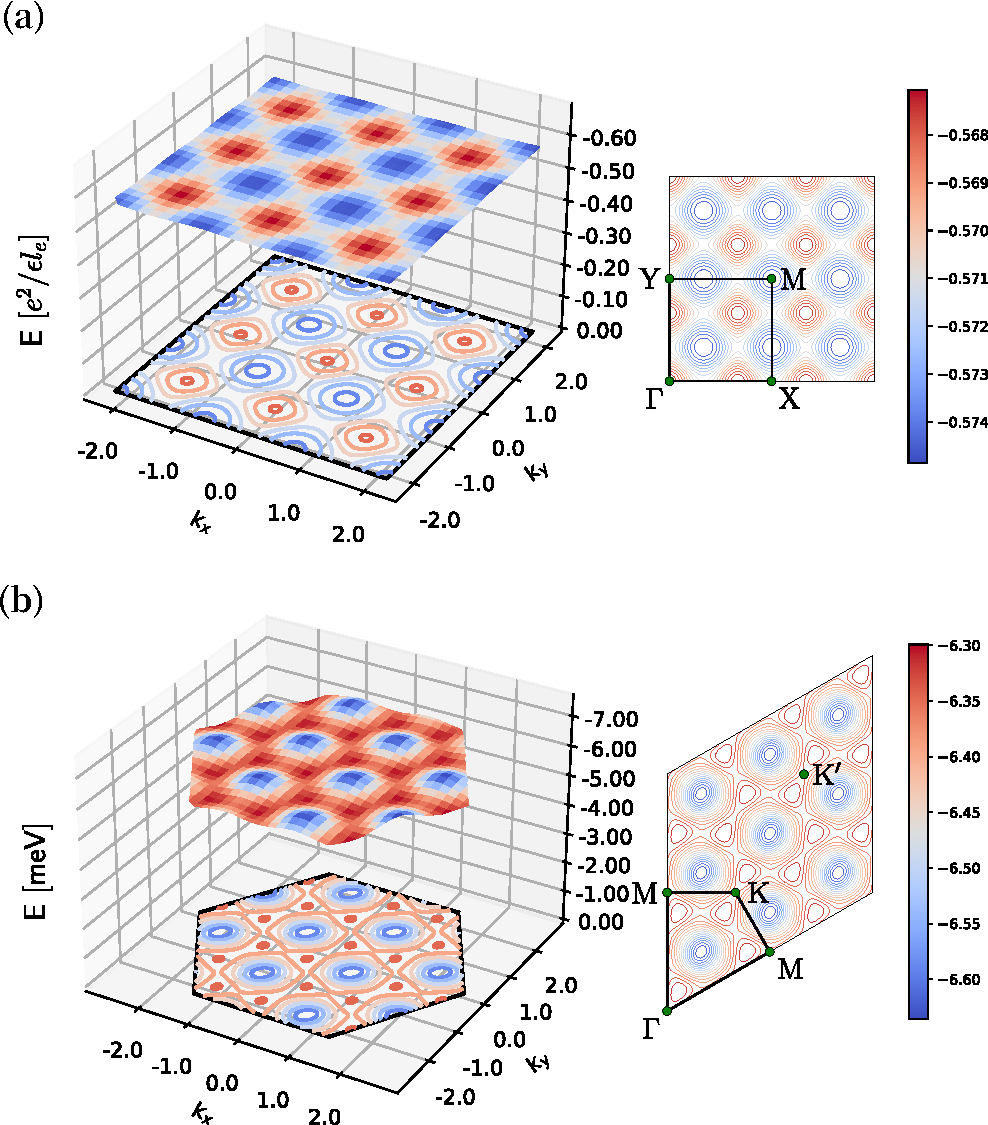
\includegraphics[width=0.85\textwidth]{figures/FCI/combined_cf_translation_fractionalization.pdf}
    \caption{Filled CF band dispersion obtained using the Hartree-Forck approximation. The calculation is done for MLL model (a) with parameter $V_{10}=0.12$ units of $\frac{e^2}{\epsilon\ell_e}$ and $\mathrm{MoTe_2}$ model (b) with parameter $\lambda=0.6$ on a $9\times9$ lattice. These Hartree-Fock CF bands turn out to be \emph{nearly flat}. As is shown in Eq.\eqref{eq: translation fractionalization}, a three-fold periodicity of CF band dispersion emerges as a manifestation of the translation-symmetry fractionalization, as is seen in both subfigures on the right. Note that we have used the \emph{electron's Brillouin Zone} (BZ) to plot the CF dispersion for better visualization of the symmetry fractionalization (in the tMoTe$_2$ model the electron's BZ is the moiré BZ.). The CF's BZ should be 1/3 of the electron's BZ due to the enlarged real-space unit cell along the $\mathbf a_1$ direction.}
    \label{fig: CF dispersion}
\end{figure}

\subsubsection{Overlap between projected wavefunctions and ED ground states}
We perform exact diagonalization (ED) on the sample of $6\times4$ unit cells with the tuning parameter: the periodic potential $V_{10}$ for MLL model, and the band scaling factor $\lambda$ for $\mathrm{tMoTe_2}$ model. The many-body spectra for selected parameter values are shown in FIG.\ref{fig: ED}. As the parameter is large enough, we observe a gap-closing phase transition ($V_{10}\sim 0.18\frac{e^2}{\epsilon l_e}$ for the MLL model and $\lambda\sim 1.0$ for the tMoTe$_2$ model).

Both the Laughlin state and our proposed projected wavefunction (in the form of \emph{combinatorial hyperdeterminants}) can be obtained by projecting the CF states back to the electronic many-body Fock space. The only difference is that for Laughlin's state \emph{non-optimized} mean-field states are used (corresponding to fully filled CF LLL), while for our projective construction, the Hartree-Fock self-consistent mean-field states $|\Psi^{MF}_{CF}\rangle$ are used (corresponding to fully filled lowest-energy CF Chern band).
\begin{figure}
    \centering
    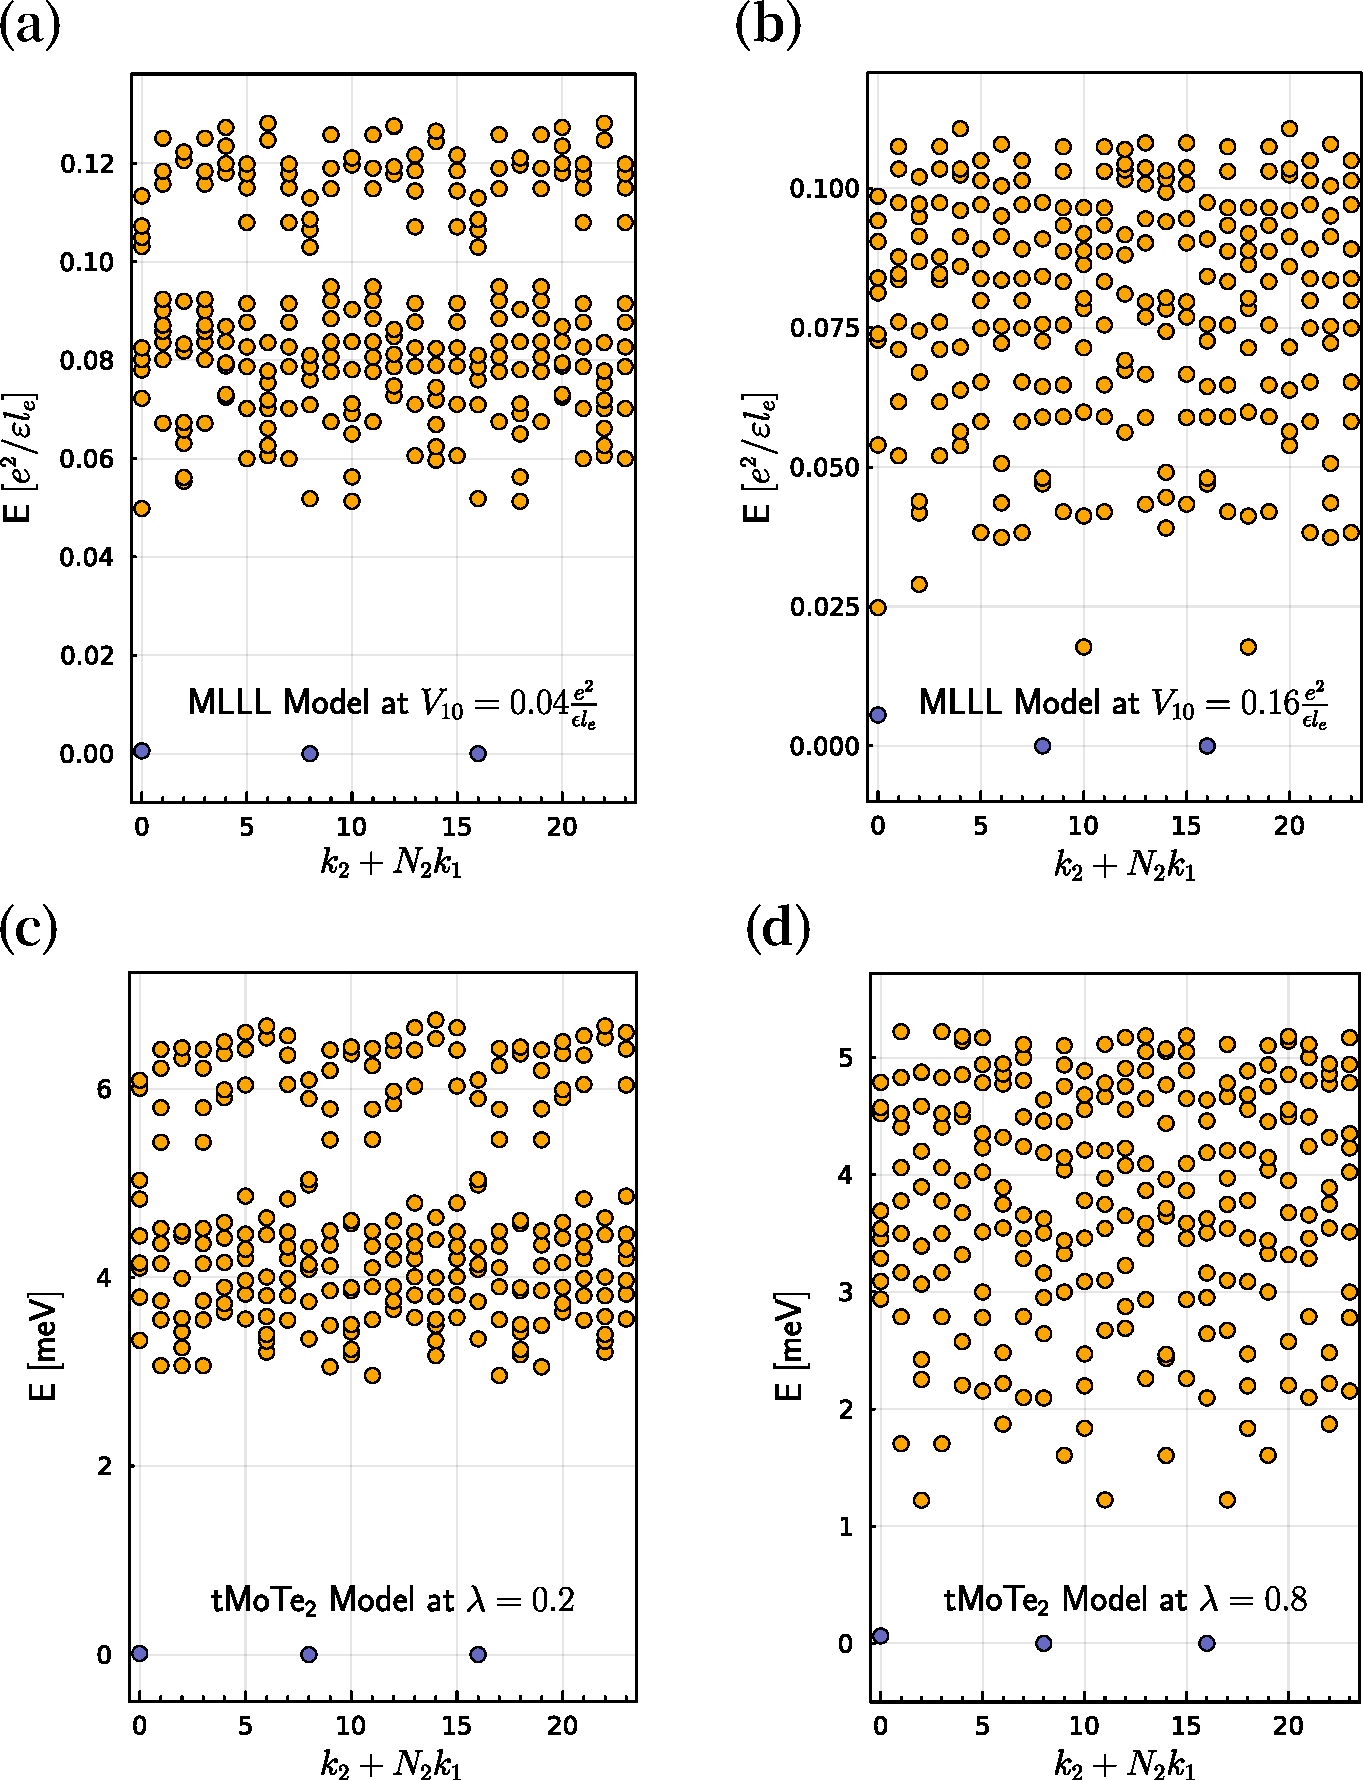
\includegraphics[width=0.9\linewidth]{figures/FCI/combined_ED.pdf}
    \caption{Selected many-body spectrum obtained from exact diagonalization on $6\times4$ unit cells. (a),(b) for MLL model and (c),(d) for $\mathrm{tMoTe_2}$ model. (a) and (c) are close to the flat band limit, while (b) and (d) have much smaller many-body gaps. The three nearly degenerate topological ground states are highlighted in dark purple.}
    \label{fig: ED}
\end{figure}


Due to the $6\times4$ system size, the projected wavefunction $\mathbf P_g|\Psi^{MF}_{CF}\rangle$ is not translational symmetric along the $\mathbf a_{1,e}$ direction with $6$ unit cells. Namely, $\mathbf P_g|\Psi^{MF}_{CF}\rangle$ is a superposition of sectors with the center of mass (COM) crystalline momentum at $\Gamma$, $\frac{1}{3}\mathbf G_{1,e}$ and $\frac{2}{3}\mathbf G_{1,e}$. When we perform the overlap calculation with the three-fold ground states obtained from ED at these three COM momenta, we use the corresponding COM sector of the same projected wavefunction $\mathbf P_g|\Psi^{MF}_{CF}\rangle$.

It turns out that, \emph{this projective construction outperforms Laughlin's states across the entire parameter space for all the three COM sectors}, as is shown in Fig.\ref{fig: ED overlap}. Notice that our optimization is performed only for the CF mean-field ground states, \emph{not} on the level of the projected electronic wavefunctions. These benchmark results indicate the present projective construction can indeed capture the microscopics of the FCI states.

\begin{figure*}
    \centering
    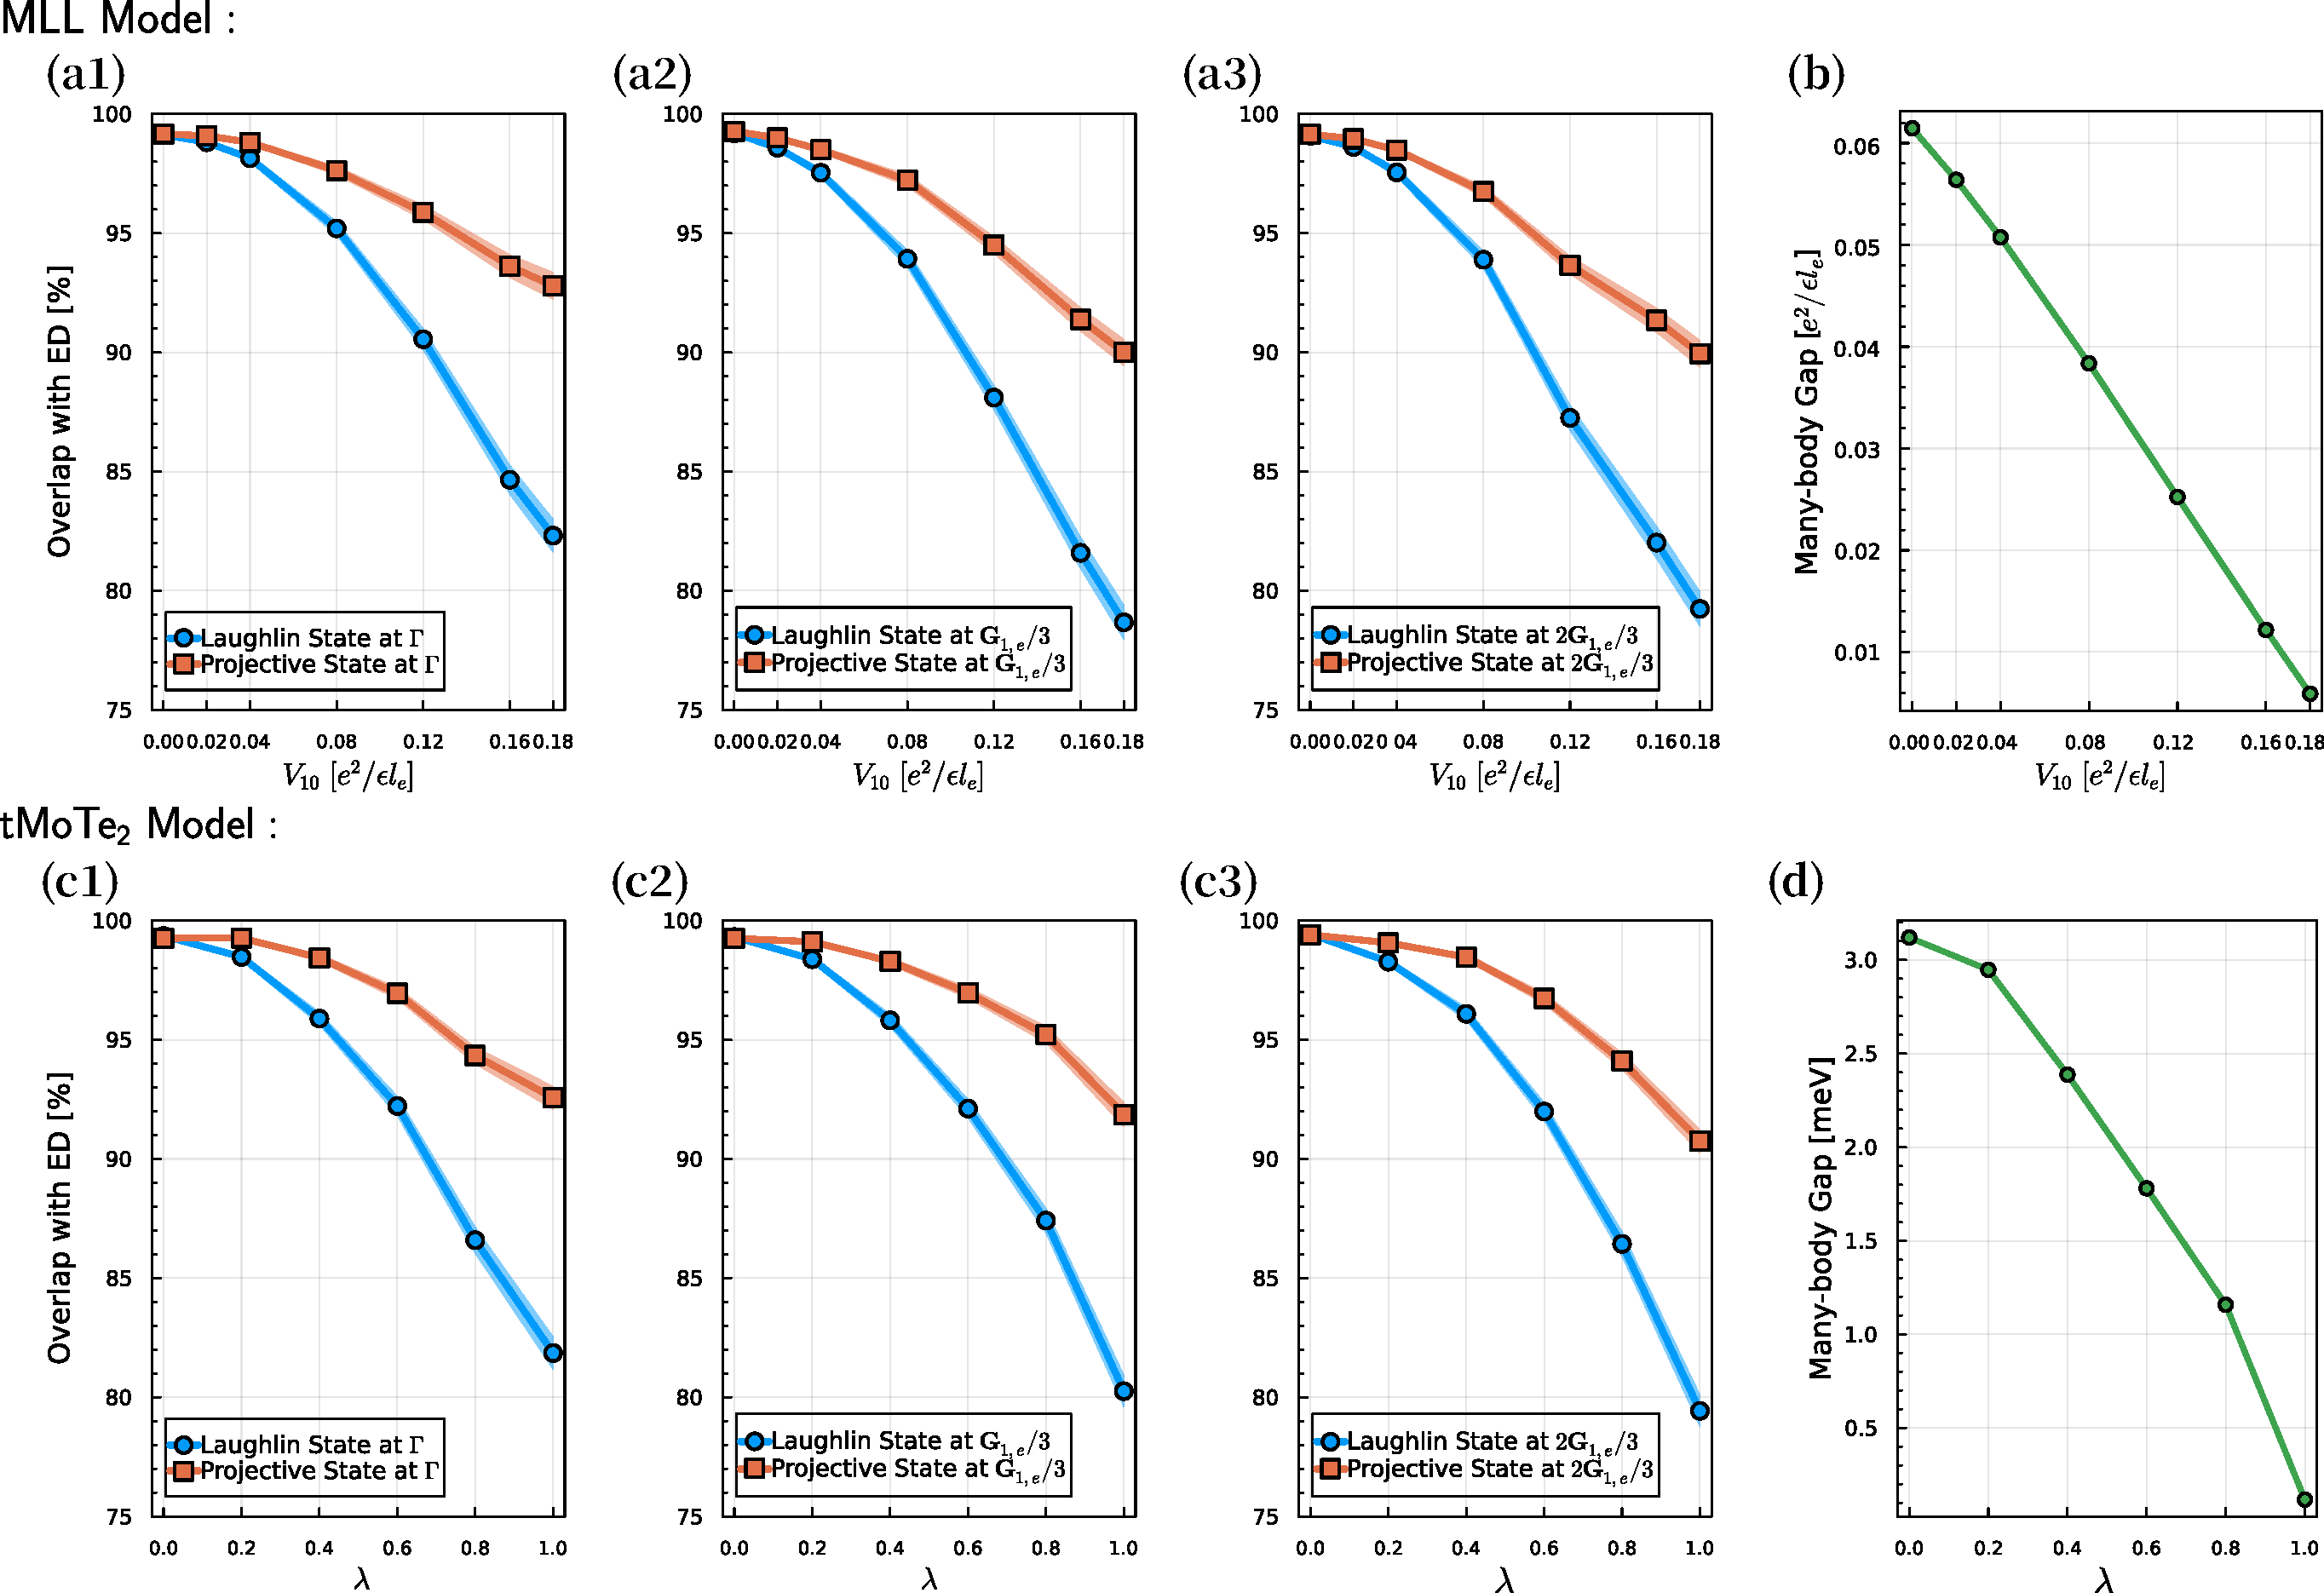
\includegraphics[width=\textwidth]{figures/FCI/combined_overlap.pdf}
    \caption{(a1)-(a3) and (c1)-(c3) exhibit the overlaps between our eletronic hyperdeterminant states and the ED ground states (red line), and the the overlaps between Laughlin's states and the ED ground states (blue line) for both MLL model and $\mathrm{tMoTe_2}$ model. Here, the overlap is defined as $|\langle \psi_{\text{ED}}|\psi_{\text{Proj}}\rangle|$ where the two wavefunctions are obtained from ED and the projective construction respectively. There exists three sectors of ground states carrying center-of-mass momentum $\Gamma, \frac{1}{3}\mathbf G_{1,e}$, and $\frac{2}{3}\mathbf G_{1,e}$ (the dark purple points in FIG.\ref{fig: ED}). The ribbon around each overlap curve represents the error bar due to variational Monte Carlo samplings. The many-body gap (i.e., the energy difference between the ground state manifold and the first excited state.) as a function of the tuning parameter is plotted in (b) and (d).}
    \label{fig: ED overlap}
\end{figure*}

\subsubsection{Magnetoroton spectra and quantum numbers}
For the samples of $6\times 6$ and $9\times9$ unit cells, we obtain the magnetoroton spectra using the time-dependent Hartree-Fock (TDHF) approximation, where eigenmodes come into pairs $\pm\hbar\omega_a(\mathbf q_e)$, with $a$ labels the magnetoroton band. The positive bands correspond to excitations above the ground state. In our TDHF calculation a nearly dispersionless CF particle-hole (PH) continuum in both models is observed, consistent with the nearly flat mean-field CF bands. This PH continuum occurs at energy $\sim 0.23 \frac{e^2}{\epsilon l_e}$ for the MLL model at $V_{10}=0.04 \frac{e^2}{\epsilon l_e}$, and at energy $\sim 11.2$meV for the tMoTe$_2$ model at $\lambda=0.2$.

Below the PH continuum, we observe four (three) branches of magnetoroton bands for the MLL (tMoTe$_2$) model. We plot the magnetoroton bands $\omega_a(\mathbf q_e)$ from the TDHF calculation in FIG.\ref{fig: magnetoroton spectrum}. In both models, \emph{the lowest energy magnetorotons are found near the BZ boundary}. The high energy magnetoroton bands (i.e., band-3 and band-4 for the MLL model and band-3 for the tMoTe$_2$ model) are visible below the PH continuum only in a small region of the BZ. Even the lowest magnetoroton band (band-1) merges into the PH continuum near the $\Gamma$-point. The rotation eigenvalues for the high-symmetry points of the magnetoroton bands are computed in Table.\ref{tab: rotation eigvals}.


\begin{figure*}[htp!]
    \centering
    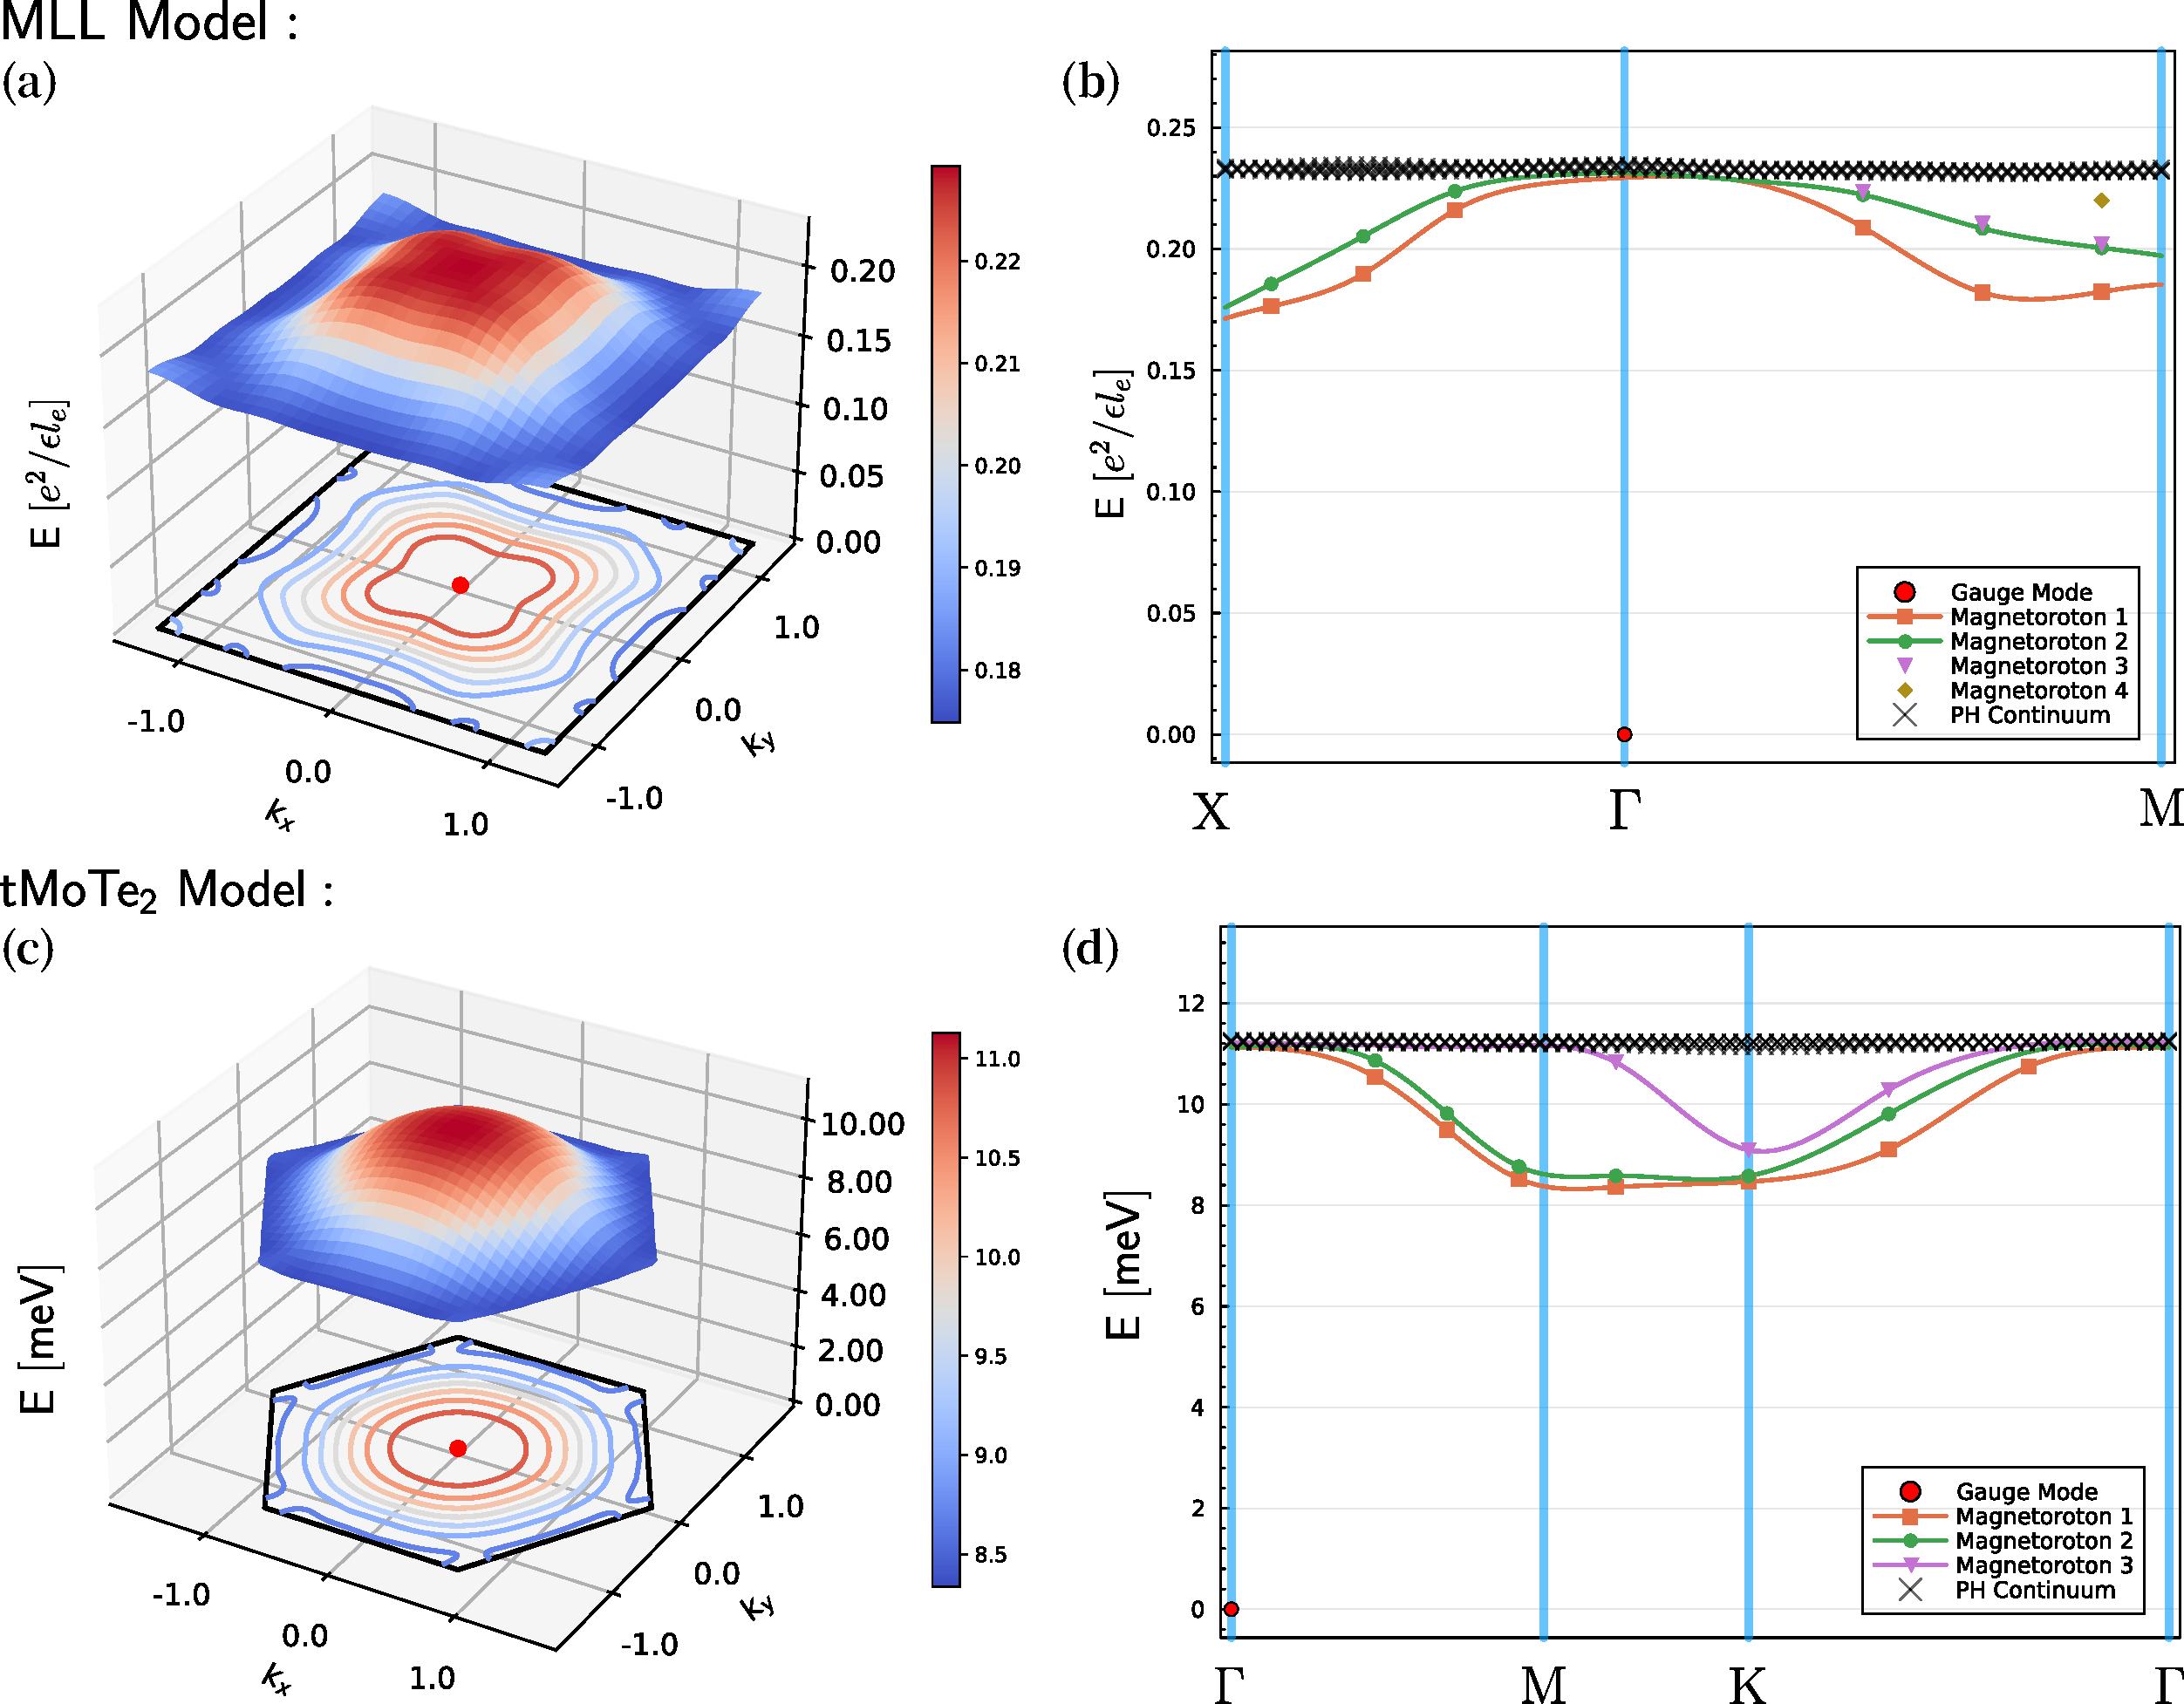
\includegraphics[width=0.95\textwidth]{figures/FCI/combined_tdhf_bands_and_surface_contour.pdf}
    \caption{Magnetoroton bands for samples of $9\times9$ unit cells obtained using the TDHF approximation. (a), (b) are for the MLL model with the parameter $V_{10}=0.04$ units of $e^2/\epsilon l_e$, and (c), (d) are for the $\mathrm{tMoTe_2}$ model with the parameter $\lambda=0.2$. (a) and (c) are the fitted 2D surface contour of the lowest magnetoroton band (band-1), while (b) and (d) exhibit the full magnetoroton spectra, where scattering points represent the raw data along the path, and the higher horizontal crosses are from the particle-hole (PH) continuum. See Fig.\ref{fig: CF dispersion} for the definitions of the high-symmetry points. Note: there is no raw data point along the $\mathrm{X}$-$\mathrm{M}$ line in the MLL model due to the choice of $9\times9$ sample size. We provide the raw data for a smaller $6\times6$ MLL sample in the Appendix. \ref{app:extended_data} for comparison. We do not perform band fitting for the magnetoroton band-3 and band-4 for the MLL model due to the limited number of points outside the PH continuum. The appearance of the nearly zero-energy modes (red dots in all four figures) at the $\Gamma$-point is due to the $\mathcal R_v$ gauge degrees of freedom discussed in the main text near the end of Sec.\ref{sec:HF_TDHF}.}
    \label{fig: magnetoroton spectrum}
\end{figure*}

\begin{table}[htp!]
    \centering
    \begin{tabular}{|| c | c | p{1.5cm} | p{1.5cm} | p{1.5cm}}
        % \hline
        % MLL model & $\Gamma:i$ & $\text{X or Y}:-1$ & $\mathrm{M}:-i$ \\
        % \hline
        % $\mathrm{tMoTe_2}$ model & $\Gamma:e^{i2\pi/3}$ & $\mathrm{K}:1$ & $\mathrm{K'}:1$ \\
        % \hline\hline
        \hline
                                 & band \# & $\Gamma$                                     & $\mathrm{X}$ or $\mathrm{Y}$                 & $\mathrm{M}$   \\
        \hline
        MLL model                & 1       & \diagbox[innerwidth=1.5cm, height=\line]{}{} & $-1$                                         & $-i$           \\
                                 & 2       & \diagbox[innerwidth=1.5cm, height=\line]{}{} & $1$                                          & $1$            \\
                                 & 3       & \diagbox[innerwidth=1.5cm, height=\line]{}{} & \diagbox[innerwidth=1.5cm, height=\line]{}{} & $-1$           \\
                                 & 4       & \diagbox[innerwidth=1.5cm, height=\line]{}{} & \diagbox[innerwidth=1.5cm, height=\line]{}{} & $i$            \\
        \hline\hline
                                 & band \# & $\Gamma$                                     & $\mathrm{K}$                                 & $\mathrm{K'}$  \\
        \hline
        $\mathrm{tMoTe_2}$ model & 1       & \diagbox[innerwidth=1.5cm, height=\line]{}{} & $1$                                          & $1$            \\
                                 & 2       & \diagbox[innerwidth=1.5cm, height=\line]{}{} & $e^{-i2\pi/3}$                               & $e^{-i2\pi/3}$ \\
                                 & 3       & \diagbox[innerwidth=1.5cm, height=\line]{}{} & $e^{i2\pi/3}$                                & $e^{i2\pi/3}$  \\
        \hline\hline
    \end{tabular}
    \caption{Rotation eigenvalues for high-symmetry points of TDHF bands. For MLL model, unlike $\Gamma$ or $\mathrm{M}$ points, the rotation eigenvalue for X and Y points are defined for $C_2$ rotation instead of $C_4$. For $\mathrm{tMoTe_2}$ model, all high symmetry points are defined for $C_3$ rotation, and the magnetorotons at $\mathrm{K}$ and $\mathrm{K'}$ points are related by the $C_{2y}\mathcal T$ symmetry \cite{wu2019topological} and thus have identical eigenvalues. Note: when the magnetoroton band merges into the particle-hole(PH) continuum, the corresponding rotation eigenvalue is not presented since one cannot separate the magnetoroton state from the PH continuum. See Fig.\ref{fig: magnetoroton spectrum} for details.}
    \label{tab: rotation eigvals}
\end{table}

We find that the energy scale of the magnetoroton excitations obtained using the TDHF approximation is larger than the excitation energy scale obtained from ED (by a factor $\sim 3$ in both models for the parameters chosen in Fig.\ref{fig: magnetoroton spectrum}). Performing the projection $\mathbf P_g$ is expected to improve the energetics significantly. Due to the complexity of the calculation, we leave computing the projected magnetoroton energies as a future project.

Finally, for the models studied here, no CF LL band inversion is observed. Namely, the FCI quantum phase remains adiabatically connected to the traditional Laughlin's wavefunctions. It would be very interesting to identify and simulate a model where CF band inversion actually occurs. We again leave this as a future direction.

\section{Discussion and Conclusions}\label{sec:conclusion}
In this paper, we present a general projective construction for the composite fermion states in a partially filled Chern band with Chern number $\pm 1$. In the context of the traditional fractional Quantum Hall liquids, the current construction clarifies a few physical puzzles and unifies several previous studies. In the context of FCI, the current construction paves a route to extract important and experimental relevant microscopic information for the FCI states, including magnetoroton spectrum, magnetoroton quantum numbers, and anyon quasiparticle band structures and  crystalline symmetry fractionalization pattern, the Fermi surface shape of the composite Fermi liquid, etc. Some of these seem difficult to access using other methods. We demonstrate how to apply our construction and extract microscopic information in some model systems, including the model for the twisted bilayer MoTe$_2$.

This work also leaves many open questions. A practical question is about the computation of a hyperdeterminant, which is known to be NP-hard. In the present work, we have used translational symmetry to slightly reduce the computational complexity. This allows us to compute hyperdeterminant exactly up to a system size comparable to those used in exact diagonalization. Is it possible to compute hyperdeterminants for larger systems? There may be two directions to proceed. First, instead of computing hyperdeterminant exactly, there may be algorithms to perform the projection approximately. Second, instead of considering the general hyperdeterminant wavefunctions, one may focus on a subclass of wavefunctions whose hyperdeterminants are easier to compute.

On the conceptual side, one open question is about the non-abelian fractional quantum Hall states. The simplest state in this regard may be the Pfaffian state obtained via pairing on the composite Fermi surface \cite{moore1991nonabelions,lee2007particle,levin2007particle,son2015composite,read2000paired}. We expect the present construction, after moderate revision, can be applied to such states in the FCI context. The mathematically relevant object is the so-called hyperpfaffian \cite{aboud2016hyperpfaffians}, which is the natural generalization of pfaffian, but defined for tensors.

Another crucial conceptual question that we did not answer in this work is the effective theories associated with the projected wavefunctions. We have demonstrated that in the context of the Galilean invariant traditional Fractional quantum Hall liquids, the projected wavefunctions in our construction are identical to those obtained by Jain's prescription, whose low energy Chern-Simons effective theories have been studied previously using various methods \cite{lopez1991fractional,zhang1992chern,lu2016classification,gromov2015framing,gromov2017bimetric,geracie2015spacetime,sohal2018chern,wen1999projective,barkeshli2010effective}. Even in this Galilean invariant case, finding the correct long-wavelength effective theories can be nontrivial. A remarkable example was established by Dong and Senthil recently \cite{dong2020noncommutative}, where they investigated the composite Fermi liquid for the $\nu=1$ bosonic system. This system has two apparently different theories: the Halperin-Lee-Read theory (HLR) theory \cite{halperin1993theory} and the Pasquier-Haldane-Read (PHR) theory \cite{pasquier1998dipole,read1998lowest}. The former theory is not within the LLL, leading to an effective theory with a Chern-Simons term. The latter theory is within the LLL, but apparently leads to an effective theory with no Chern-Simons term. Dong and Senthil showed that the effective theory of PHR is defined in a noncommutative space. After approximately mapping to a commutative field theory, the same Chern-Simon term as HLR emerges.

The present construction includes the effects of the crystalline potential and generally applies to Jain's sequence and the composite Fermi liquid in FCI systems. Similar to the PHR theory, our construction is explicitly within the partially filled Chern band. The HLR theory, however, is parallel to the usual parton construction \emph{without} projecting into the Chern band (see Eq.(\ref{eq:usual_parton})). We leave the investigation of the long-wavelength effective theories for the proposed projected wavefunctions in future works.


\vspace{1em}
\noindent\emph{Acknowledgement.---} We thank Senthil Todadri, Ashvin Vishwanath, Yong Baek Kim and Yuan-Ming Lu for helpful discussions. We acknowledge the HPC resources from Andromeda cluster at Boston College.  D.X. acknowledges support from the Center on Programmable Quantum Materials, an Energy Frontier Research Center funded by DOE BES under award DE-SC0019443.


\vspace{1em}
\noindent\emph{Note added.---} After the completion of the manuscript, we became aware that Junren Shi \cite{shi2023quantum} generalizes the Pasquier-Haldane-Read’s construction for the $\nu=1$ bosonic composite Fermi liquid to the case of Galilean invariant $\nu=1/2$ fermionic composite Fermi liquid in the disc geometry, where a projection to the $\nu=1/2$ bosonic Laughlin state in the vortex space is used, and coincides with our construction in this case.




\begin{subappendices}
    \section{The rotation transformations of LLL bloch states and the CB-LLL mapping}\label{app:mag_rot}
    Let us consider a 2D rotation symmetric sample with $e^{i\theta}\mathbf a_{i,e}= \sum_j r_{ij}\mathbf a_{j,e}$ and $N_{1,e}=N_{2,e}\equiv N$, where $r_{ij}\in\mathbb Z$ and $i,j\in\{1,2\}$. Choosing $z_0=\mathbf a_{i,e}$ in Eq.(\ref{eq:R_T_identity}), then
    \begin{align}
         & D_e(\mathbf a_{i,e})=[U_{R,e}(\theta)R_e(\theta)]^{-1} D_e(e^{i\theta}\mathbf a_{i,e})[U_{R,e}(\theta)R_e(\theta)]\notag \\
         & \quad=[U_{R,e}(\theta)R_e(\theta)]^{-1} D_e(\sum_{ij}\mathbf a_{j,e})[U_{R,e}(\theta)R_e(\theta)].
    \end{align}
    Applying to the bloch basis $|\mathbf k_e\rangle_{\text{LLL}}$, and expanding $D_e(\sum_{ij}\mathbf a_j)$ using the GMP algebra
    \begin{align}
        D_e(\sum_j r_{ij}\mathbf a_{j,e})=e^{i\pi r_{i1}r_{i2}}D_e( r_{i1}\mathbf a_{1,e})D_e( r_{i2}\mathbf a_{2,e}),
    \end{align}
    we have
    \begin{align}
        e^{-i \mathbf k_e\cdot \mathbf a_{i,e}}=e^{i\pi r_{i1}r_{i2}} e^{-i (R_{\theta}\mathbf k_e)\cdot  (e^{i\theta}\mathbf a_{i,e})}.
    \end{align}


    Using the identity $(-1)^{r_{i1}+r_{i2}+1}=(-1)^{r_{i1}r_{i2}}$ (because $r_{i1},r_{i2}$ cannot be both even, since $\det(r_{ij})=1$), and noting that $e^{-i \mathbf k_e\cdot \mathbf a_{i,e}}\equiv e^{-i (e^{i\theta}\mathbf k_e)\cdot (e^{i\theta}\mathbf a_{i,e})}$, one can obtain the expression:
    \begin{align}
        e^{-i (R_{\theta}\mathbf k_e)\cdot  (e^{i\theta}\mathbf a_{i,e})} & =e^{-i (e^{i\theta}(\mathbf k_e-\mathbf K_e)+\mathbf K_e)\cdot (e^{i\theta}\mathbf a_{i,e})},\notag \\
        \text{where }\mathbf K_e                                          & \equiv \frac{\mathbf G_{1,e}}{2}+\frac{\mathbf G_{2,e}}{2}.
    \end{align}

    Therefore, generally speaking, the rotation should be viewed as about the $[\pi,\pi]$-point $\mathbf K_e$ of the BZ. For the $C_2$ and $C_4$ systems, the phase factor $e^{i\pi r_{i1}r_{i2}}$ is trivial and the rotation can also be viewed as about the $[0,0]$-point. However, for the $C_3$ and $C_6$ systems, this phase factor is nontrivial, and one does need to view the rotation as about the $[\pi,\pi]$-point (or momentum points differ by a reciprocal lattice vector). \emph{To have a uniform discussion, in this paper we always view the rotation as about the $[\pi,\pi]$-point in the LLL.}

    Choosing $z_0=\frac{\mathbf a_{i,e}}{N}$ in Eq.(\ref{eq:R_T_identity}), we have:
    \begin{align}
         & [U_{R,e}(\theta)R_e(\theta)]\rho_e(\tfrac{\mathbf G_{1,e}}{N})[U_{R,e}(\theta)R_e(\theta)]^{-1}\notag                                                                            \\
         & \quad\quad=\rho_e(e^{i\theta}\tfrac{\mathbf G_{1,e}}{N})=e^{i\pi\frac{r_{21}r_{22}}{N^2}}\rho_e(r_{22}\tfrac{\mathbf G_{1,e}}{N})\rho_e(-r_{21}\tfrac{\mathbf G_{2,e}}{N})\notag \\
         & [U_{R,e}(\theta)R_e(\theta)]\rho_e(\tfrac{\mathbf G_{2,e}}{N})[U_{R,e}(\theta)R_e(\theta)]^{-1}\notag                                                                            \\
         & \quad\quad=\rho_e(e^{i\theta}\tfrac{\mathbf G_{2,e}}{N})=e^{i\pi\frac{r_{11}r_{12}}{N^2}}\rho_e(-r_{12}\tfrac{\mathbf G_{1,e}}{N})\rho_e(r_{11}\tfrac{\mathbf G_{2,e}}{N})
    \end{align}
    Applying to Eq.(\ref{eq:rho_matrix_element}), one obtains:
    \begin{align}
         & e^{i\xi(\theta,\mathbf k_e+\frac{\mathbf G_{1,e}}{N})} e^{i\frac{\mathbf k_e\cdot\mathbf a_{2,e}}{N}}\notag                                                               \\
         & \qquad=e^{i\pi\frac{r_{21}r_{22}}{N^2}}e^{ir_{22}\frac{(R_{\theta}\mathbf k_e-r_{21}\frac{\mathbf G_{2,e}}{N})\cdot\mathbf a_{2,e}}{N}}e^{i\xi(\theta,\mathbf k_e)}\notag \\
         & e^{i\xi(\theta,\mathbf k_e+\frac{\mathbf G_{2,e}}{N})}\notag                                                                                                              \\
         & \qquad=e^{i\pi\frac{r_{11}r_{12}}{N^2}}e^{-ir_{12}\frac{(R_{\theta}\mathbf k_e+r_{11}\frac{\mathbf G_{2,e}}{N})\cdot\mathbf a_{2,e}}{N}}e^{i\xi(\theta,\mathbf k_e)}.
    \end{align}
    Namely:
    \begin{align}
        e^{i\xi(\theta,\mathbf k_e+\frac{\mathbf G_{1,e}}{N})} & =e^{-i\pi\frac{r_{21}r_{22}}{N^2}}e^{-i\frac{\mathbf k_e\cdot\mathbf a_{2,e}}{N}}e^{ir_{22}\frac{R_{\theta}\mathbf k_e\cdot\mathbf a_{2,e}}{N}}e^{i\xi(\theta,\mathbf k_e)}\notag \\
        e^{i\xi(\theta,\mathbf k_e+\frac{\mathbf G_{2,e}}{N})} & =e^{-i\pi\frac{r_{11}r_{12}}{N^2}}e^{-ir_{12}\frac{R_{\theta}\mathbf k_e\cdot\mathbf a_{2,e}}{N}}e^{i\xi(\theta,\mathbf k_e)}.
    \end{align}
    These equations fully determine $e^{i\xi(\theta,\mathbf k_e)}$ up to an overall shift, which can be fixed by computing $e^{i\xi(\theta,\mathbf 0)}$.

    For instance, for a $C_4$ symmetric lattice, the matrix $(r_{ij})=i\sigma_y$, $R_{\theta}\mathbf{k}_e\equiv R_\theta(k_1 \frac{\mathbf G_{1,e}}{2\pi} + k_2 \frac{\mathbf G_{2,e}}{2\pi})=((-k_2+2\pi) \frac{\mathbf G_{1,e}}{2\pi} + k_1 \frac{\mathbf G_{2,e}}{2\pi})$, one finds:
    \begin{align}
        C_4:\; e^{i\xi(\frac{\pi}{2},\mathbf k_e)}=e^{-i \frac{k_1 k_2}{2\pi}}.
    \end{align}
    Using the BZ boundary condition Eq.(\ref{eq:BZ_BC}), the rotation eigenvalues are:
    \begin{align}
         & C_4 \text{ systems: }\notag                                      \\
         & \quad\quad C_4([(0,0)\text{ shifted by }(\pi,\pi)])=(-i), \notag \\
         & \quad\quad C_4([(\pi,\pi)\text{ shifted by }(\pi,\pi)])=1,\notag \\
         & \quad\quad C_2([(\pi,0)\text{ shifted by }(\pi,\pi)])=1.
    \end{align}

    For a $C_6$ symmetric lattice, we choose $\mathbf a_{2,e}=e^{i\frac{2\pi}{3}}\mathbf a_{1,e}$ and the $(r_{ij})$ matrix becomes $\begin{pmatrix} 1& 1 \\ -1 & 0\end{pmatrix}$. Consequently $\mathbf G_{2,e}=e^{i\frac{\pi}{3}}\mathbf G_{1,e}$. As is mentioned before, the rotation center is shifted to $[\pi,\pi]$, so $R_\theta\mathbf k_e\equiv R_{\theta} (k_1 \frac{\mathbf G_{1,e}}{2\pi} + k_2 \frac{\mathbf G_{2,e}}{2\pi})=(-(k_2-\pi)+\pi) \frac{\mathbf G_{1,e}}{2\pi} + ((k_1-\pi)+(k_2-\pi)+\pi) \frac{\mathbf G_{2,e}}{2\pi}=(-k_2+2\pi) \frac{\mathbf G_{1,e}}{2\pi} + (k_1+k_2-\pi) \frac{\mathbf G_{2,e}}{2\pi}$, and one finds:
    \begin{align}
        C_6:\; e^{i\xi(\frac{\pi}{3},\mathbf k_e)}=e^{-i\frac{\pi}{12}}e^{-i \frac{k_1 k_2+\frac{1}{2}k_2(k_2-2\pi)}{2\pi}}.
    \end{align}
    The rotation eigenvalues are:
    \begin{align}
         & C_6\text{ systems: }\notag                                                               \\
         & \quad\quad C_6([(0,0)\text{ shifted by }(\pi,\pi)])=e^{-i\frac{\pi}{3}},\notag           \\
         & \quad\quad C_3([(\tfrac{2\pi}{3},\tfrac{2\pi}{3})\text{ shifted by }(\pi,\pi)])=1,\notag \\
         & \quad\quad C_2([(\tfrac{\pi}{2},0)\text{ shifted by }(\pi,\pi)])=1.
    \end{align}
    The rotation transformation for $C_2$ and $C_3$ can be obtained by the square of the $C_4$ and $C_6$. These results show that in the LLL, the magnetic rotation eigenvalues are $e^{-i\theta}$ at the $\mathbf K_e=(\pi,\pi)$-point, and are trivial everywhere else.

    In a general Chern band, The Chern number put a constraint on the rotation eigenvalues at these high-symmetry points \cite{fang2012bulk}:
    \begin{align}
         & C_2 \text{ systems }:\notag                                                                                                         \\
         & (-1)^C=C_2[(0,0)]\cdot C_2[(\pi,\pi)]\cdot C_2[(\pi,0)]\cdot C_2[(0,\pi)]\notag                                                     \\
         & C_4 \text{ systems }:\notag                                                                                                         \\
         & e^{i\frac{\pi}{2}C}=(-1)^F C_4[(0,0)]\cdot C_4[(\pi,\pi)]\cdot C_2[(\pi,0)]\notag                                                   \\
         & C_3 \text{ systems }:\notag                                                                                                         \\
         & e^{i\frac{2\pi}{3}C}=(-1)^F C_3[(0,0)]\cdot C_3[(\frac{2\pi}{3},\frac{2\pi}{3})]\cdot C_3[-(\frac{2\pi}{3},\frac{2\pi}{3})]\notag   \\
         & C_6 \text{ systems }:\notag                                                                                                         \\
         & e^{i\frac{\pi}{3}C}=(-1)^F C_6[(0,0)]\cdot C_3[(\frac{2\pi}{3},\frac{2\pi}{3})]\cdot C_2[(\frac{\pi}{2},0)],\label{eq:C_constraint}
    \end{align}
    where $(C_n)^n=(-1)^F$. Here, we have $C=-1$ and choose the convention that $(-1)^F=1$. It is straightforward to redefine the rotation operation to describe the case of $(-1)^F=-1$.

    Due to the mapping Eq.(\ref{eq:CB_LLL_map}), we know that if the CB has a rotation eigenvalue $e^{-i\theta}$ at the $\Gamma$-point and trivial everywhere else (coined ``\emph{the fundamental case}'' below), a smooth gauge satisfying Eq.(\ref{eq:CB_BZ_BC},\ref{eq:CB_rotation}) can be found following the prescription of Ref.\cite{jian2013crystal}. If the rotation eigenvalues do not match the fundamental case, one needs to redefine the rotation operation $R_{\text{CB}}(\theta)$ following two steps as below, without changing the algebra satisfied by $R_{\text{CB}}(\theta)$ and $T_{\text{CB}}(\mathbf a_{i,e})$.

    In the first step, one redefines $R_{\text{CB}}(\theta)$ by multiplying a factor $e^{-im\theta}$ ($m\in\mathbb Z$): $R_{\text{CB}}(\theta)\rightarrow e^{-im\theta}R_{\text{CB}}(\theta)$, so that the eigenvalue $C_n[(0,0)]=e^{-i\theta}$, matching the fundamental case. This step induces a possible nontrivial Wen-Zee shift. After this step, the eigenvalues at the other high-symmetry points still may not match the fundamental case, in which case we need the second step.

    In the second step, we redefine $R_{\text{CB}}(\theta)$ by combining a translation. For example, for $C_4$ systems, after the first step, it is possible that $C_4[(\pi,\pi)]=C_2[(\pi,0)]=-1$. In this case, one redefine $R_{\text{CB}}(\theta)\rightarrow T_{\text{CB}}(\mathbf a_{1,e})R_{\text{CB}}(\theta)$, and the redefined rotation eigenvalues match the fundamental case. Physically, if $R_{\text{CB}}(\theta)$ is the $C_4$ rotation about a square lattice site, then $T_{\text{CB}}(\mathbf a_{1,e})R_{\text{CB}}(\theta)$ is the $C_4$ rotation about a plaquette center. Similar redefinitions can be made for $C_2$ (using either the link center or the plaquette center rotations) and $C_3$ systems (using the plaquette center rotation). For $C_6$ systems, the second step is not needed since one must have $C_3[(\frac{2\pi}{3},\frac{2\pi}{3})]=C_2[(\frac{\pi}{2},0)]=1$ after the first step. After these two steps of redefinition, a complete match with the fundamental case can always be made.

    \section{Composite fermion substitution for the case of $\nu=\frac{1}{2s}$ composite Fermi liquid}\label{app:CFL_substitution}
    In the case of $\nu=\frac{1}{2s}$, the bosonic vortex carries $q_v=-q_e$, and forms a $\nu=\frac{1}{2s}$ fractional quantum hall liquid. This corresponds to the $p\rightarrow\infty$ case of the Jain's sequence. In the disc geometry with the open boundary condition, $\mathcal R_e$ and $\mathcal R_v$ satisfies the algebra:
    \begin{align}
        [\mathcal R_{e,x},\mathcal R_{e,y}] & =-il_e^2, & [\mathcal R_{v,x},\mathcal R_{v,y}] & =il_e^2.
    \end{align}
    They can be used to construct the charge-neutral composite fermion variables:
    \begin{align}
        r_x & =\frac{1}{2}(\mathcal R_{e,x}+\mathcal R_{v,x})\notag      \\
        r_y & =\frac{1}{2}(\mathcal R_{e,y}+\mathcal R_{v,y})\notag      \\
        k_x & =\frac{-1}{l_e^2}(\mathcal R_{e,y}-\mathcal R_{v,y})\notag \\
        k_y & =\frac{1}{l_e^2}(\mathcal R_{e,x}-\mathcal R_{v,x})
    \end{align}
    It is straightforward to check that these CF variables satisfy $[r_x,k_x]=[r_y,k_y]=i$, while all other commutators vanish. Note that $\bm k$ can be represented as:
    \begin{align}
        \bm k=\frac{1}{l_e^2}\hat z\times(\mathcal R_e-\mathcal R_v),
    \end{align}
    indicating that the CF's momentum is related to its electric dipole moment.

    On a finite size system with $N_{1,e}\cdot N_{2,e}$ unit cells, one may choose either the real-space or momentum-space basis for the CF. For example, the momentum-space basis is given by the eigenstates of the translation operator:
    \begin{align}
        T_{CF}(z)=e^{-i\bm k\cdot z}=D_e(z)\cdot D_v(z)
    \end{align}
    The boundary-condition-allowed $z$ is given by $z=l_2\frac{\mathbf a_{1,e}}{N_{2,e}}-l_1\frac{\mathbf a_{2,e}}{N_{1,e}}$, $l_i\in \mathbb Z$. And the physically distinct $\bm k$ eigenvalues are:
    \begin{align}
        \bm k= (m_{1}+\frac{\varphi_{1,e}-\varphi_{1,v}}{2\pi})\frac{\mathbf G_{1,e}}{N_{1,e}}+(m_{2}+\frac{\varphi_{2,e}-\varphi_{2,v}}{2\pi})\frac{\mathbf G_{2}}{N_{2,e}},
    \end{align}
    where $m_i\in [0,N_{1,e}\cdot N_{2,e}-1]$ are integers. Since the number of fluxes $N_{\phi,e}=N_{\phi,v}=N_{1,e}\cdot N_{2,e}$, one finds that these $N_{\phi,e}^2$ number of momentum eigenstates exactly reproduce the dimension of the Hilbert space $\mathcal H_e\otimes \mathcal H_v$.

    In the presence of crystalline potential, these momentum eigenstates will hybridize and form the CF band structure with the Brillion Zone characterized by $\mathbf G_{i,e}$, and each band has $N_{\phi,e}$ momentum points. On the mean-field level, the composite Fermi liquid is formed by filling the lowest (mean-field) energy band by the filling fraction $\frac{1}{2s}$. This CFL mean-field state can then be fed into the projector $\mathbf P_g$ to obtain the projected electronic wavefunction, which is still a hyperdeterminant.

    \section{Density operator expectation values in Laughlin states on the torus}\label{app:density_expectation}
    The discussion here largely follows Ref.\cite{wen1990ground}, apart from the numerical results. It is known that Laughlin's states at $\nu=1/m$ form a $m$-fold irreducible representation of the many-body magnetic translation algebra on a torus:
    \begin{align}
        \pmb{\bm D}_e(z_1)\pmb{\bm D}_e(z_2) & =e^{\frac{i}{2} \frac{z_1\times z_2}{l_e^2} N_e}\pmb{\bm D}_e(z_1+z_2)\notag \\
                                             & =e^{i \frac{z_1\times z_2}{l_e^2} N_e} \pmb{\bm D}_e(z_2)\pmb{\bm D}_e(z_1)
    \end{align}
    For convenience of discussion below, we introduce the minimal translation displacement $\delta_1$ ($\delta_2$) along the $L_1$ ($L_1\tau$) direction of the sample that is consistent with the torus boundary condition.
    \begin{align}
        \delta_1\equiv & \frac{L_{1}}{N_{\phi,e}}, & \delta_2\equiv & \frac{L_{1}\tau}{N_{\phi,e}},
    \end{align}
    leading to
    \begin{align}
        \pmb{\bm D}_e(\delta_1)\pmb{\bm D}_e(\delta_2)=e^{i\frac{2\pi}{m}}\pmb{\bm D}_e(\delta_2)\pmb{\bm D}_e(\delta_1).
    \end{align}
    One can choose a gauge for the $m$-fold Laughlin's states $|\psi_i\rangle$ ($i \in [0,m-1]$) as the eigenstates of $\pmb{\bm D}_e(\delta_1)$, satisfying:
    \begin{align}
        \pmb{\bm D}_e(\delta_1)|\psi_i\rangle & =e^{i\phi_1}e^{i\frac{2\pi i}{m}}|\psi_i\rangle, & \pmb{\bm D}_e(\delta_2)|\psi_i\rangle & =|\psi_{i+1}\rangle,\label{eq:Laughlin_gauge}
    \end{align}
    where $|\psi_{i+m}\rangle\equiv e^{i\phi_2}|\psi_{i}\rangle$ and the phase factors $e^{i\phi_i}$ depend on the boundary condition.

    The many-particle density operator satisfies a relation with the magnetic translation operator:
    \begin{align}
        \pmb{\bm D}_e(z_0) \pmb{\boldsymbol\rho}_e(\mathbf q_e=\frac{iz_1}{l_e^2}) \pmb{\bm D}_e(z_0)^\dagger=e^{i\frac{z_0\times z_1}{l_e^2}}\pmb{\boldsymbol\rho}_e(\mathbf q_e=\frac{iz_1}{l_e^2}).
    \end{align}
    Plugging in $z_0=m\delta_1$ or $z_0=m\delta_2$, using Eq.(\ref{eq:Laughlin_gauge}), the above identity leads to:
    \begin{align}
         & \langle \psi_i|\pmb{\boldsymbol\rho}_e(\mathbf q_e)|\psi_j\rangle\neq 0 \notag                                    \\
         & \text{ only if } \mathbf q_e=\mathbf q_e(n_1,n_2)\equiv\frac{i (n_1 \frac{L_1}{m}+ n_2\frac{L_1\tau}{m})}{l_e^2},
    \end{align}
    where $n_i\in [0,m-1]$ are integers.

    Let's define the operators:
    \begin{align}
        \mathbf A(n_1,n_2)\equiv \pmb{\bm D}_e(n_1\delta_1+n_2\delta_2)^{-1} \pmb{\boldsymbol\rho}_e(\mathbf q_e(n_1,n_2)).\label{eq:A_def}
    \end{align}
    One can show that $\mathbf A(n_1,n_2)$ commutes with both $\pmb{\bm D}_e(\delta_1)$ and $\pmb{\bm D}_e(\delta_2)$, and consequently must be a constant in the ground state manifold.


    \begin{table}
        \centering
        \vspace{2mm}
        \begin{tabular}{||c | c | c | c | c||}
            \hline
            $N_\phi$ & $\tau=i$    & $\tau=e^{i\frac{2\pi}{3}}$ \\
            \hline\hline
            2        & 1           & 1                          \\\hline
            4        & -$\sqrt{2}$ & -1.156(1)                  \\\hline
            6        & 1.267(1)    & 1.000(1)                   \\\hline
            8        & -0.8652(4)  & -0.5591(7)                 \\\hline
            10       & 0.5658(7)   & 0.3273(7)                  \\\hline
            12       & -0.3423(8)  & -0.1831(9)                 \\\hline
            14       & 0.1993(8)   & 0.0932(5)                  \\\hline
            16       & -0.1139(3)  & -0.0461(3)                 \\\hline
            18       & 0.0641(4)   & 0.0228(2)                  \\\hline
            \hline
        \end{tabular}
        \caption{$\mathbf A(n_1=1,n_2=0)$ (see Eq.(\ref{eq:A_def})) for Laughlin's $\nu=1/2$ state, with the sample shape parameter $\tau=i$ and $\tau=e^{i\frac{2\pi}{3}}$, and boundary condition $\varphi_{1,e}=\varphi_{2,e}=0$ (see Eq.(\ref{eq:boundary_conditions})).}
        \label{tb:rho_v_expectation}
    \end{table}

    We have checked numerically that $A(n_1,n_2)\sim e^{-c \cdot N_{\varphi,e}}$ in the ground state manifold exponentially decay in the thermodynamic limit ($c$ is a constant for a given $\tau$ and boundary condition.). For instance, in Table.\ref{tb:rho_v_expectation} we list the values of $\mathbf A(n_1=1,n_2=0)$ in the ground state manifold for Laughlin's $\nu=1/2$ states (electron is bosonic), computed via variational Monte Carlo.

    \section{Time-dependent Hartree-Fock approximation in the presence of constraints}\label{app:TDHF}
    Here we describe the general prescription to compute the excitation spectrum in the framework of TDHF in the presence of constraints and Lagrange multipliers. The original many-body Hamiltonian $\mathbf H=\mathbf H_0+\mathbf V$, where $\mathbf H_0$ is the two-body term. For simplicity, we consider $\mathbf V$ as the density-density interaction:
    \begin{align}
        \mathbf V=\frac{1}{2}\sum_{\mathbf q} V_{\mathbf q} \pmb{\boldsymbol\rho}(\mathbf q)\pmb{\boldsymbol\rho}(-\mathbf q),
    \end{align}
    where $\pmb{\boldsymbol\rho}(\mathbf q)$ is a fermion bilinear. We assume a collection of linearly independent Hermitian symmetry generators $\{\mathbf S_i\}$ that are fermion bilinears. They commute with $\mathbf H$, and form a closed algebra:
    \begin{align}
        [\mathbf S_i,\mathbf H]   & =0,\;\forall i,\notag                             \\
        [\mathbf S_i,\mathbf S_j] & =i\sum_{k} c_{ijk}\mathbf S_k\label{eq:S_algebra}
    \end{align}
    In the main text, the symmetry generators $\{\mathbf S_i\}$ are vortices density operators $\{\pmb{\boldsymbol\rho}_v(\mathbf q_v)\}$.

    The mean-field \emph{free-fermion states} $|\psi\rangle$'s under consideration are those that satisfy the constraints:
    \begin{align}
        \langle \psi |\mathbf S_i| \psi\rangle =0.\;\forall i\label{eq:S_constraints}
    \end{align}
    $|\psi\rangle$ is completely captured by its single-body density matrix:
    \begin{align}
        \boldsymbol{\mathcal P}\equiv \sum_{\alpha,\beta}\langle \psi| f_{\beta}^\dagger f_{\alpha}|\psi\rangle f_{\alpha}^\dagger f_{\beta},
    \end{align}
    where $\alpha,\beta$ labels a basis in the single-particle Hilbert space.

    For any single-body density matrix $\boldsymbol{\mathcal P}$, we define the Hartree-Fock approximated Hamiltonian:
    \begin{align}
        \mathbf H_{HF}(\boldsymbol{\mathcal P})\equiv \mathbf H_0+\mathbf V_{HF}(\boldsymbol{\mathcal P}),
    \end{align}
    where
    \begin{align}
        \mathbf V_{HF}(\boldsymbol{\mathcal P}) & \equiv \frac{1}{2} \sum_{{\mathbf q}}V_{\mathbf q}\bigg[ \mathop{\mathrm{Tr}}[\pmb{\boldsymbol\rho}(\mathbf q)\boldsymbol{\mathcal P}]\pmb{\boldsymbol\rho}(-\mathbf q)+\pmb{\boldsymbol\rho}(\mathbf q)\mathop{\mathrm{Tr}}[\pmb{\boldsymbol\rho}(-\mathbf q)\boldsymbol{\mathcal P}]\notag \\
                                                & \quad-\pmb{\boldsymbol\rho}(\mathbf q)\boldsymbol{\mathcal P}\pmb{\boldsymbol\rho}(-\mathbf q)-\pmb{\boldsymbol\rho}(-\mathbf q)\boldsymbol{\mathcal P}\pmb{\boldsymbol\rho}(\mathbf q) \bigg].
    \end{align}

    The standard static Hartree-Fock calculation boils down to finding $\boldsymbol{\mathcal P}_0$ that minimizes the variational energy $\langle\psi|\mathbf H|\psi\rangle$, subject to the constraints Eq.(\ref{eq:S_constraints}). One can show that under a small perturbation $\boldsymbol{\mathcal P}_0\rightarrow \boldsymbol{\mathcal P}_0+\delta\boldsymbol{\mathcal P}$, the linear order change of variational energy is:
    \begin{align}
        0=\delta\langle\psi|\mathbf H|\psi\rangle=\mathop{\mathrm{Tr}}[\mathbf H_{HF}(\boldsymbol{\mathcal P}_0)\delta\boldsymbol{\mathcal P}].
    \end{align}
    Quite generally, such a small perturbation can be parameterized by a small unitary rotation $\boldsymbol{\mathcal P}_0\rightarrow \mathbf U\boldsymbol{\mathcal P}_0\mathbf U^\dagger$ where $\mathbf U=e^{i\boldsymbol\phi}$, $\boldsymbol\phi$ is a small fermion bilinear operator. To the leading order, $\delta\boldsymbol{\mathcal P}=i[\boldsymbol\phi,\boldsymbol{\mathcal P}_0]$, so
    \begin{align}
        0=i\mathop{\mathrm{Tr}}[\mathbf H_{HF}(\boldsymbol{\mathcal P}_0)[\boldsymbol\phi,\boldsymbol{\mathcal P}_0]]=-i\mathop{\mathrm{Tr}}[\boldsymbol\phi[\mathbf H_{HF}(\boldsymbol{\mathcal P}_0),\boldsymbol{\mathcal P}_0]],\label{eq:P0_condition}
    \end{align}
    where we have used the trace identity $\mathop{\mathrm{Tr}}[\mathbf A[\mathbf B,\mathbf C]]=\mathop{\mathrm{Tr}}[\mathbf B[\mathbf C,\mathbf A]]$.

    At this point, it is helpful to introduce the symplectic structure of the space of the fermion bilinear operators. We can separate any fermion bilinear operator $\mathbf A$ into two parts:
    \begin{align}
        \mathbf A            & =\{\mathbf A\}_{phys}+\{\mathbf A\}_{unphys},\;\;\text{where}\notag                                                                               \\
        \{\mathbf A\}_{phys} & \equiv [[\mathbf A,\boldsymbol{\mathcal P}_0],\boldsymbol{\mathcal P}_0]\notag                                                                    \\
                             & =(\mathbf 1-\boldsymbol{\mathcal P}_0)\mathbf A\boldsymbol{\mathcal P}_0+\boldsymbol{\mathcal P}_0\mathbf A(\mathbf 1-\boldsymbol{\mathcal P}_0).
    \end{align}
    Using the fact that $\boldsymbol{\mathcal P}_0$ is a projector, one can easily show that $[\mathbf A,\boldsymbol{\mathcal P}_0]=[\{\mathbf A\}_{phys},\boldsymbol{\mathcal P}_0]$. Namely, to consider the small unitary rotation above, it is sufficient to consider the linear space spanned by $\{\mathbf A\}_{phys}$, which we denote as $\boldsymbol{\mathcal W}$. Note that for one has $[\mathbf A,\boldsymbol{\mathcal P}_0]\in \boldsymbol{\mathcal W},\; \forall \text{ fermion bilinear } \mathbf A$, and there is a useful identity:
    \begin{align}
        \mathop{\mathrm{Tr}}[\boldsymbol{\mathcal P}_0[\mathbf A,\mathbf B]]=\mathop{\mathrm{Tr}}[\boldsymbol{\mathcal P}_0[\{\mathbf A\}_{phys},\{\mathbf B\}_{phys}]]
    \end{align}

    In $\boldsymbol{\mathcal W}$, we can define two different inner products. The first (single angle bracket) is a conventional one while the second (double angle bracket) is a symplectic one.
    \begin{align}
        \langle \{\mathbf A\}_{phys},\{\mathbf B\}_{phys}\rangle  & \equiv\mathop{\mathrm{Tr}}[ \{\mathbf A^\dagger\}_{phys}\cdot \{\mathbf B\}_{phys}]\notag                              \\
        \llangle\{\mathbf A\}_{phys},\{\mathbf B\}_{phys}\rrangle & \equiv\mathop{\mathrm{Tr}}[ \{\mathbf A^\dagger\}_{phys}\cdot [ \{\mathbf B\}_{phys},\boldsymbol{\mathcal P}_0]]\notag \\
                                                                  & =\mathop{\mathrm{Tr}}[\boldsymbol{\mathcal P}_0 [ \{\mathbf A^\dagger\}_{phys},\{\mathbf B\}_{phys}]].
    \end{align}

    The condition that $\delta \boldsymbol{\mathcal P}$ does not change the constraint relations Eq.(\ref{eq:S_constraints}) can also be written as $-i\mathop{\mathrm{Tr}}[\boldsymbol{\mathcal P}_0[\mathbf S_i,\boldsymbol{\phi}]]=0$, or in terms of the symplectic inner product introduced above:
    \begin{align}
        \llangle\{\mathbf S_i\}_{phys},\{\boldsymbol\phi\}_{phys}\rrangle=0.
    \end{align}
    We may denote the subspace in $\boldsymbol{\mathcal W}$ spanned by $\{\mathbf S_i\}_{phys}$ as $\boldsymbol{\mathcal W}_{\mathbf S}$. The above condition means that $\{\boldsymbol\phi\}_{phys}\in \overline{\boldsymbol{\mathcal W}_{\mathbf S}}$, where $\overline{\boldsymbol{\mathcal W}_{\mathbf S}}$ is the symplectic complement of $\boldsymbol{\mathcal W}_{\mathbf S}$. Drastically different from the conventional complement subspace, here we have:
    \begin{align}
        \boldsymbol{\mathcal W}_{\mathbf S} \subset \overline{\boldsymbol{\mathcal W}_{\mathbf S}},
    \end{align}
    which is a consequence of Eq.(\ref{eq:S_algebra}). The variational minimization problem now becomes finding $\boldsymbol{\mathcal P}_0$ so that Eq.(\ref{eq:P0_condition}) is satisfied for all $\boldsymbol\phi\in\overline{\boldsymbol{\mathcal W}_{\mathbf S}}$.

    If the objective was to find $\boldsymbol{\mathcal P}_0$ so that Eq.(\ref{eq:P0_condition}) is satisfied for all $\boldsymbol\phi$ in the \emph{entire space} $\boldsymbol{\mathcal W}$, then it would lead to the well-known self-consistent condition $[\mathbf H_{HF}(\boldsymbol{\mathcal P}_0),\boldsymbol{\mathcal P}_0]=0$. However, since $\overline{\boldsymbol{\mathcal W}_{\mathbf S}}$ is smaller than $\boldsymbol{\mathcal W}$, as long as $[\mathbf H_{HF}(\boldsymbol{\mathcal P}_0),\boldsymbol{\mathcal P}_0]\in \overline{\boldsymbol{\mathcal W}_{\mathbf S}}^\perp$, $\boldsymbol{\mathcal P}_0$ is a legitimate optimal solution to satisfy Eq.\eqref{eq:P0_condition} satisfied. Here $\overline{\boldsymbol{\mathcal W}_{\mathbf S}}^\perp$ is the conventional complement subspace of $\overline{\boldsymbol{\mathcal W}_{\mathbf S}}$ (Here and below we always use ${\;\cdot\;}^\perp$ to denote the conventional complement and $\overline{\;\cdot\;}$ to denote the symplectic complement).

    One can show that $\overline{\boldsymbol{\mathcal W}_{\mathbf S}}^\perp$ is actually the symplectic dual of the subspace $\boldsymbol{\mathcal W}_{\mathbf S}$. Namely, they are orthogonal to each other w.r.t. the conventional inner product, have the same dimension, and the linear map $\mathbf x\mapsto [\mathbf x,\boldsymbol{\mathcal P}_0]$ is a one-to-one mapping between the two subspaces. One way to see this is to decompose $\overline{\boldsymbol{\mathcal W}_{\mathbf S}}$ into the direct sum of two mutually orthogonal subspaces (w.r.t. the conventional inner product): $\overline{\boldsymbol{\mathcal W}_{\mathbf S}}=\boldsymbol{\mathcal W}_{\mathbf S}\oplus \boldsymbol{\mathcal V}$. It follows that, by definition, $\boldsymbol{\mathcal W}$ is the direct sum of three mutually orthogonal (w.r.t. the conventional inner product) subspaces:
    \begin{align}
        \boldsymbol{\mathcal W}=\boldsymbol{\mathcal W}_{\mathbf S}\oplus\overline{\boldsymbol{\mathcal W}_{\mathbf S}}^\perp\oplus\boldsymbol{\mathcal V}\label{eq:W_decomposition}
    \end{align}
    Now by choosing an arbitrary $\mathbf x\in \boldsymbol{\mathcal W}_{\mathbf S}$, from above decomposition we know $\llangle \boldsymbol{\mathcal W}_{\mathbf S},\mathbf x\rrangle=\llangle \boldsymbol{\mathcal V},\mathbf x\rrangle=0$, i.e., $\langle \boldsymbol{\mathcal W}_{\mathbf S},[\mathbf x,\boldsymbol{\mathcal P}_0]\rangle=\langle \boldsymbol{\mathcal V},[\mathbf x,\boldsymbol{\mathcal P}_0]\rangle=0$. Thus we must have $[\mathbf x,\boldsymbol{\mathcal P}_0]\in \overline{\boldsymbol{\mathcal W}_{\mathbf S}}^\perp$. Noting that $[[\mathbf x,\boldsymbol{\mathcal P}_0],\boldsymbol{\mathcal P}_0]=\mathbf x$, we showed that $\mathbf x\mapsto [\mathbf x,\boldsymbol{\mathcal P}_0]$ is a one-to-one mapping between $\boldsymbol{\mathcal W}_{\mathbf S}$ and $\overline{\boldsymbol{\mathcal W}_{\mathbf S}}^\perp$. This mapping also sends $\boldsymbol{\mathcal V}$ back to $\boldsymbol{\mathcal V}$.

    Therefore, there exist a collection of Lagrange multipliers $\lambda_i$, so that $[\mathbf H_{HF}(\boldsymbol{\mathcal P}_0),\boldsymbol{\mathcal P}_0]=-[\sum_i\lambda_i\mathbf S_i,\boldsymbol{\mathcal P}_0]$. This is equivalent to the condition:
    \begin{align}
        [\mathbf{\tilde H}_{HF}(\boldsymbol{\mathcal P}_0), \boldsymbol{\mathcal P}_0]\equiv\bigg[\mathbf H_{HF}(\boldsymbol{\mathcal P}_0)+\sum_i\lambda_i\mathbf S_i, \boldsymbol{\mathcal P}_0\bigg]=0.
    \end{align}
    This is the well-known prescription: one can introduce Lagrange multipliers so that the ground state of $\mathbf{\tilde H}_{HF}(\boldsymbol{\mathcal P}_0)$ satisfies the constraints Eq.(\ref{eq:S_constraints}), and perform the self-consistent calculation as usual.

    Now we are ready to study the time-evolution of the single-body density matrix near $\boldsymbol{\mathcal P}_0$:
    \begin{align}
        [\mathbf{\tilde H}_{HF}(\boldsymbol{\mathcal P}), \boldsymbol{\mathcal P}]=i\hbar\dot{\boldsymbol{\mathcal P}}
    \end{align}
    To the linear order of $\boldsymbol\phi$, this leads to:
    \begin{align}
         & [\mathbf {\tilde H}_{HF}(\boldsymbol{\mathcal P}_0),[\boldsymbol\phi,\boldsymbol{\mathcal P}_0]]+[\mathbf V_{HF}([\boldsymbol\phi,\boldsymbol{\mathcal P}_0]),\boldsymbol{\mathcal P}_0]\notag \\
         & \quad+(-i)\left[\sum_i\delta\lambda_i(\boldsymbol\phi) \mathbf S_i,\boldsymbol{\mathcal P}_0\right]=i\hbar [\dot{\boldsymbol\phi},\boldsymbol{\mathcal P}_0].
    \end{align}
    $\delta\lambda_i(\boldsymbol\phi)\propto \boldsymbol\phi$ is the adjustment of the Lagrange multipliers due to $\boldsymbol\phi$, so that the ground state of $\mathbf{\tilde H}_{HF}(\boldsymbol{\mathcal P})$ satisfies the constraints Eq.(\ref{eq:S_constraints}).
    Equivalently, we can define the operator $\boldsymbol{\mathcal H}$:
    \begin{align}
        \boldsymbol{\mathcal H} \cdot \{\boldsymbol\phi\}_{phys} & \equiv [[\mathbf {\tilde H}_{HF}(\boldsymbol{\mathcal P}_0),\{\boldsymbol\phi\}_{phys}],\boldsymbol{\mathcal P}_0]\notag     \\
                                                                 & \quad+[\mathbf V_{HF}([\{\boldsymbol\phi\}_{phys},\boldsymbol{\mathcal P}_0]),\boldsymbol{\mathcal P}_0], \label{eq:H_eigen}
    \end{align}
    and introduce the linear operator $\boldsymbol{\mathcal L}$ to represent the eigen equation (using Jacobi identity and static condition)
    \begin{align}
        \boldsymbol{\mathcal L}\cdot \{\boldsymbol\phi\}_{phys} & \equiv [\boldsymbol{\mathcal H} \cdot \{\boldsymbol\phi\}_{phys},\boldsymbol{\mathcal P}_0]+(-i)\sum_i\delta\lambda_i(\boldsymbol\phi) \{\mathbf S_i\}_{phys}\notag \\
                                                                & =i\hbar\{\dot{\boldsymbol\phi}\}_{phys}=\hbar\omega\{\boldsymbol\phi\}_{phys} .\label{eq:L_eigen}
    \end{align}

    One can show that if $\{\boldsymbol\phi\}_{phys}\in \overline{\boldsymbol{\mathcal W}_{\mathbf S}}$, then $\boldsymbol{\mathcal L}\cdot \{\boldsymbol\phi\}_{phys}\in \overline{\boldsymbol{\mathcal W}_{\mathbf S}}$ as well. To see this, it is sufficient to show $[\boldsymbol{\mathcal H} \cdot \{\boldsymbol\phi\}_{phys},\boldsymbol{\mathcal P}_0]\in \overline{\boldsymbol{\mathcal W}_{\mathbf S}}$, or equivalently $\boldsymbol{\mathcal H} \cdot \{\boldsymbol\phi\}_{phys}\in \boldsymbol{\mathcal W}_{\mathbf S}^{\perp}$.

    In fact, one can show that the operator $\boldsymbol{\mathcal H}$ is Hermitian (w.r.t the conventional inner product) in the full space $\boldsymbol{\mathcal W}$. It the follows that $\forall i$ and $\{\boldsymbol\phi\}_{phys}\in \overline{\boldsymbol{\mathcal W}_{\mathbf S}}$,
    \begin{align}
        \langle \{\mathbf S_i\}_{phys},\boldsymbol{\mathcal H} \cdot \{\boldsymbol\phi\}_{phys}\rangle=\langle \{\boldsymbol\phi\}_{phys},\boldsymbol{\mathcal H} \cdot \{\mathbf S_i\}_{phys} \rangle^*=0
    \end{align}
    This is because
    \begin{align}
        \boldsymbol{\mathcal H} \cdot \{\mathbf S_i\}_{phys} \in \overline{\boldsymbol{\mathcal W}_{\mathbf S}}^\perp,\label{eq:H_S}
    \end{align}
    as a consequence of the symmetry, which we will explain next.

    TDHF is known to be a conserving approximation. For instance, the Goldstone mode computed in TDHF is gapless. This can be demonstrated explicitly. A symmetry generator $\mathbf S_i$ should satisfy both $[\mathbf S_i,\mathbf H_0]=0$ and $[\mathbf S_i,\mathbf V]=0$. The latter condition leads to an important identity:
    \begin{align}
        [\mathbf S_i,\mathbf V_{HF}(\boldsymbol{\mathcal P})]=\mathbf V_{HF}([\mathbf S_i,\boldsymbol{\mathcal P}])
    \end{align}
    Therefore, if $\boldsymbol{\mathcal P}_0$ is a static Hartree-Fock solution with Lagrange multipliers $\lambda_j$, then $e^{i\epsilon \mathbf S_i}\boldsymbol{\mathcal P}_0 e^{-i\epsilon \mathbf S_i}$ is automatically another static Hartree-Fock solution with Lagrange multipliers unitary rotated by $e^{i\epsilon \mathbf S_i}$. One finds that
    \begin{align}
        \boldsymbol{\mathcal L}\cdot\{\mathbf S_i\}_{phys}=0, \text{ with } \delta\lambda_j(\mathbf S_i)=\sum_k c_{kij}\lambda_k
    \end{align}
    Namely, each $\mathbf S_i$ corresponds to an exact zero mode -- the Goldstone mode. This result in turn tells that $[\boldsymbol{\mathcal H} \cdot \{\mathbf S_i\}_{phys},\boldsymbol{\mathcal P}_0]\in\boldsymbol{\mathcal W}_{\mathbf S}$, which, under the one-to-one correspondence $\mathbf x\mapsto[\mathbf x,\boldsymbol{\mathcal P}_0], \boldsymbol{\mathcal W}_{\mathbf S}\rightarrow\overline{\boldsymbol{\mathcal W}_{\mathbf S}}^\perp$, also establishes the validity of Eq.(\ref{eq:H_S}).

    We are now ready to find all the eigen modes in TDHF. Note the decomposition of $\boldsymbol{\mathcal W}$ in Eq.(\ref{eq:W_decomposition}). We should solve the eigenproblem of $\boldsymbol{\mathcal L}$ in
    $\overline{\boldsymbol{\mathcal W}_{\mathbf S}}=\boldsymbol{\mathcal W}_{\mathbf S}\oplus \boldsymbol{\mathcal V}$, and the subspace $\boldsymbol{\mathcal W}_{\mathbf S}$ is the null space of $\boldsymbol{\mathcal L}$. One then only needs to consider the operator $\boldsymbol{\mathcal L}$ in the subspace $\boldsymbol{\mathcal V}$, where the eigenvalues are generically nonzero. Introducing the projector $\mathbf P_{\boldsymbol{\mathcal V}}$ into the subspace $\boldsymbol{\mathcal V}$, we need to solve the eigenproblem for the operator $\boldsymbol{\mathcal L}_{\boldsymbol{\mathcal V}}$:
    \begin{align}
         & \boldsymbol{\mathcal L}_{\boldsymbol{\mathcal V}}\cdot\boldsymbol{\phi}=[\boldsymbol{\mathcal H}_{\boldsymbol{\mathcal V}}\cdot\boldsymbol{\phi},\boldsymbol{\mathcal P}_0],\notag                                                                                                                                                                       \\
         & \text{where }\boldsymbol{\mathcal L}_{\boldsymbol{\mathcal V}}\equiv \mathbf P_{\boldsymbol{\mathcal V}}\cdot\boldsymbol{\mathcal L}\cdot\mathbf P_{\boldsymbol{\mathcal V}}\text{ and }\boldsymbol{\mathcal H}_{\boldsymbol{\mathcal V}}\equiv \mathbf P_{\boldsymbol{\mathcal V}}\cdot\boldsymbol{\mathcal H}\cdot\mathbf P_{\boldsymbol{\mathcal V}}.
    \end{align}
    If $\boldsymbol{\mathcal L}_{\boldsymbol{\mathcal V}}\cdot \boldsymbol\phi =\hbar\omega \boldsymbol\phi $ with $\omega\neq 0$ for $\boldsymbol\phi\in \boldsymbol{\mathcal V}$, one can always extend $\boldsymbol\phi$ to $\overline{\boldsymbol{\mathcal W}_{\mathbf S}}$ by adding a unique component in $\boldsymbol{\mathcal W}_{\mathbf S}$ so that Eq.(\ref{eq:L_eigen}) holds.

    The eigenproblem of $\boldsymbol{\mathcal L}_{\boldsymbol{\mathcal V}}$ can be shown to be equivalent to diagonalizing a free boson Hamiltonian via the bosonic Bogoliubov transformation (i.e., symplectic transformation): the eigenvalues are real and appear as $\pm \hbar\omega$ pairs. This is because $\boldsymbol{\mathcal H}_{\boldsymbol{\mathcal V}}$ satisfies the following conditions:
    \begin{align}
        \boldsymbol{\mathcal H}_{\boldsymbol{\mathcal V}}\cdot \boldsymbol{\phi}^\dagger=(\boldsymbol{\mathcal H}_{\boldsymbol{\mathcal V}}\cdot \boldsymbol{\phi})^\dagger,
    \end{align}
    which can be easily seen from Eq.(\ref{eq:H_eigen}) using $[\mathbf A^\dagger,\mathbf B^\dagger]\equiv-[\mathbf A,\mathbf B]^\dagger$. Consequently, if $\boldsymbol{\mathcal L}_{\boldsymbol{\mathcal V}}\boldsymbol{\phi}=\hbar\omega \boldsymbol{\phi}$, then $\boldsymbol{\mathcal L}_{\boldsymbol{\mathcal V}}\boldsymbol{\phi}^\dagger=-\hbar\omega \boldsymbol{\phi}^\dagger$.

    Let's summary some main results here. Let the dimension of the linear space $\boldsymbol{\mathcal W}$ be $D_{\boldsymbol{\mathcal W}}$. In the energy eigenbasis of $\tilde {\mathbf H}_{HF}(\boldsymbol{\mathcal P}_0)$, $\boldsymbol{\mathcal W}$ is spanned by the fermion bilinears $c_{\alpha}^{\dagger} d_{i}$ and $d_{i}^{\dagger} c_{\alpha}$, where $i$ labels the filled single-particle orbitals and $\alpha$ labels the empty single-particle orbitals. Only these bilinears have nontrivial commutator with $\boldsymbol{\mathcal P}_0$. Therefore $D_{\boldsymbol{\mathcal W}}=2\cdot N_{filled}\cdot N_{empty}$, where $N_{filled}$ ($N_{empty}$) is the number of filled (empty) single-particle orbitals.

    In the presence of $N_c$ constraints, the perturbations corresponding to violation of the constraints span a subspace $\overline{\boldsymbol{\mathcal W}_{\mathbf S}}^\perp$, which is $N_c$ dimensional. The exact zero energy Goldstone modes, span a subspace $\boldsymbol{\mathcal W}_{\mathbf S}$, which is also $N_c$ dimensional. The nonzero energy modes can be found by studying the subspace $\boldsymbol {\mathcal V}$, which is $D_{\boldsymbol{\mathcal W}}-2\cdot N_c$ dimensional. $\boldsymbol{\mathcal W}$ has the important decomposition Eq.(\ref{eq:W_decomposition}).


    \section{Derivation of Eq.\eqref{eq:coherent state projected to LLL} and Eq.\eqref{eq:coherent_state_fusion}}\label{app:coherent_state_fusion}
    We always work within the symmetric gauge in this appendix. First of all, let us prove Eq.\eqref{eq:coherent state projected to LLL}. The basic idea is to realize that the Dirac delta function at the origin carries zero angular momentum $L_z=a_\eta^\dagger a_\eta - a_R^\dagger a_R=0$, so that the non-vanishing expansion of it comes from states with equal $n_R$ and $n_\eta$:
    \begin{equation}
        |0_{CF}\rangle=\sum_n (-1)^n|n_R,n_\eta\rangle,
    \end{equation}
    which can be seen from the known Laguerre polynomial wavefunctions of $| n_{\mathcal R}\rangle|n_{\eta}\rangle$:
    \begin{align}\label{eq:coherent state Laguerre polynomials}
        \langle\zeta_{CF}| n_{\mathcal R}\rangle|n_{\eta}\rangle=(-1)^nL_n\left(\frac{|\zeta|^2}{2l_{CF}^2}\right) e^{-\frac{|\zeta|^2}{4l_{CF}^2}}.
    \end{align}

    So the projection to $n$-th LL reads
    \begin{align}
         & |n_\eta\rangle\langle n_\eta|\zeta_{CF}\rangle=|n_\eta\rangle\langle n_\eta|\hat T(\zeta)|0_{CF}\rangle\nonumber                       \\
         & = |n_\eta\rangle\langle n_\eta| D_R(\zeta/2)D_\eta(\zeta/2)|0_{CF}\rangle\nonumber                                                     \\
         & =|n_\eta\rangle\langle n_\eta| D_R(\zeta/2)D_\eta(\zeta/2) e^{\frac{i}{2l_{CF}^2}(\zeta_x\hat y-\zeta_y\hat x)}|0_{CF}\rangle\nonumber \\
         & =|n_\eta\rangle\langle n_\eta| D_R(\zeta/2)D_\eta(\zeta/2) D_R(\zeta/2)D_\eta(-\zeta/2)|0_{CF}\rangle\nonumber                         \\
         & =D_R(\zeta)|n_\eta\rangle\langle n_\eta|0_{CF}\rangle\nonumber                                                                         \\
         & =(-1)^n|n_\eta\rangle D_R(\zeta)|n_R\rangle.
    \end{align}
    Here, in the second line, we use an identity of the \emph{usual} translation operator $\hat T(\zeta)$ introduced in Eq.\eqref{eq:op id: D_R(z)D_eta(-z)=T(2z)}, and in the third line we insert an identity using the exponential operator (since the position operator is vanishing when acting on $|0_{CF}\rangle$), and in the fourth line we use the operator identity Eq.\eqref{eq:op id: D_R(z)D_eta(-z)=exp(...)}. Thus Eq.\eqref{eq:coherent state projected to LLL} is established.


    Following the notation in Eq.(\ref{eq:coherent_state_fusion}) in the main text, we will first compute a simpler fusion coefficient:
    \begin{align}
        A(\zeta)\equiv\langle\zeta_{CF}| 0_e\rangle|0_v\rangle.
    \end{align}
    Notice that the bosonic Bogoliubov transformation Eq.(\ref{eq:a_bogoliubov}) is generated by the unitary:
    \begin{align}
        U(c)\equiv e^{\text{arctanh}(c) (a_e^\dagger a_v^\dagger-a_ea_v)}=e^{\text{arctanh}(c) (a_{\mathcal R}^\dagger a_{\eta}^\dagger-a_{\mathcal R}a_{\eta})}.
    \end{align}
    $U(c)$ satisfies $U(c)^\dagger=U(-c)$ and:
    \begin{align}
        U(c) a_e U(c)^\dagger & =a_{\mathcal R}, & U(c) a_v U(c)^\dagger & =a_{\eta},
    \end{align}
    We thus have the relation between the coherent states and the occupation number basis:
    \begin{align}
        |0_e\rangle|0_v\rangle=U(-c)|0_{\mathcal R}\rangle|0_\eta\rangle=\sqrt{1-c^2}\sum_{n=0}^{\infty} (-c)^n|n_{\mathcal R}\rangle|n_\eta\rangle,
    \end{align}
    leading to:
    \begin{align}
        A(\zeta)=\sqrt{1-c^2}\sum_n (-c)^n\langle\zeta_{CF}| n_{\mathcal R}\rangle|n_{\eta}\rangle
    \end{align}
    where zero angular momentum wavefunctions $\langle\zeta_{CF}|n_R,n_\eta\rangle$ are the Laguerre polynomials \eqref{eq:coherent state Laguerre polynomials}.
    % It is known that the relevant wavefunctions in the CF space are the Laguerre polynomials:
    % \begin{align}
    % \langle\zeta_{CF}| n_{\mathcal R}\rangle|n_{\eta}\rangle=(-1)^nL_n\left(\frac{|\zeta|^2}{2l_{CF}^2}\right) e^{-\frac{|\zeta|^2}{4l_{CF}^2}}.
    % \end{align}
    In addition, the Laguerre polynomials have the generating function:
    \begin{align}
        \sum_n t^n L_n(x)=\frac{1}{1-t}e^{-\frac{tx}{1-t}}.
    \end{align}

    In the current situation, $t=c$, and one has:
    \begin{align}
        A(\zeta)= & \sqrt{1-c^2}\frac{1}{1-c} \exp\left[-\frac{c}{1-c}\frac{|\zeta|^2}{2l_{CF}^2}-\frac{|\zeta|^2}{4l_{CF}^2}\right]\notag \\
        =         & \sqrt{\frac{1+c}{1-c}}\exp\Big[-\Big(\frac{1+c}{1-c}\Big)\frac{|\zeta|^2}{4l_{CF}^2}\Big]
    \end{align}

    Next, we compute the complex conjugate of Eq.(\ref{eq:coherent_state_fusion}):
    \begin{align}
        B(z,\omega,\zeta)\equiv\langle\zeta_{CF}|z_e\rangle|\omega_v\rangle=\langle\zeta_{CF}|D_{e}(z) D_{v}(\omega)|0_e\rangle|0_v\rangle.\label{eq:B_definition}
    \end{align}
    Using Eq.(\ref{eq:D_e_D_v_to_D_R_D_eta}), one can show:
    \begin{align}
        D_{e}(z) D_{v}(\omega)=D_{\mathcal R}(X)D_\eta(Y).
    \end{align}
    where
    \begin{align}
        X & \equiv\frac{z-c^2\omega}{1-c^2}, & Y & \equiv\frac{c(\omega-z)}{1-c^2}.
    \end{align}
    Introducing:
    \begin{align}
        s & \equiv\frac{X+Y}{2}, & d & \equiv\frac{X-Y}{2},
    \end{align}
    one has:
    \begin{align}
         & D_{e}(z) D_{v}(\omega)\notag                                                                                                                        \\
         & =\Theta\left(\frac{d}{\sqrt{2}l_{CF}},\frac{2s}{\sqrt{2}l_{CF}}\right) D_{\mathcal R}(d)D_{\eta}(-d)D_{\mathcal R}(s)D_{\eta}(s),\label{eq:D_e_D_v}
    \end{align}
    where we have defined the phase factor involved in the magnetic translation algebra:
    \begin{align}
        \Theta(\alpha,\beta)\equiv e^{\frac{\alpha\bar\beta-\bar\alpha\beta}{2}},
    \end{align}
    whose exponent is bilinear in $\alpha,\beta$ and satisfies:
    \begin{align}
        \Theta(\alpha,\beta)          & =\bar \Theta(\beta,\alpha)\notag \\
        \Theta(\bar \alpha,\bar\beta) & =\bar \Theta(\alpha,\beta).
    \end{align}
    For instance:
    \begin{align}
        D_e(z_0)D_e(z_1)           & =\Theta\left(\frac{\bar z_0}{\sqrt 2l_e},\frac{\bar z_1}{\sqrt 2l_e}\right)D_e(z_0+z_1)\notag      \\
        D_v(\omega_0)D_v(\omega_1) & =\Theta\left(\frac{\omega_0}{\sqrt 2l_v},\frac{\omega_1}{\sqrt 2l_v}\right)D_v(\omega_0+\omega_1).
    \end{align}

    Finally, in the symmetric gauge:
    \begin{align}
        \eta_x       & =\frac{\hat x}{2}-l^2_{CF} \hat k_y, & \eta_y       & =\frac{\hat y}{2}+l^2_{CF} \hat k_x,\notag \\
        \mathcal R_x & =\frac{\hat x}{2}+l^2_{CF} \hat k_y, & \mathcal R_y & =\frac{\hat y}{2}-l^2_{CF} \hat k_x.\notag \\
    \end{align}
    leading to the operator identities:
    \begin{align}
        D_{\mathcal R}(z) D_{\eta}(-z) & =e^{\frac{i}{l_{CF}^2}(x\hat y-y\hat x)}\label{eq:op id: D_R(z)D_eta(-z)=exp(...)} \\
        D_{\mathcal R}(z) D_{\eta}(z)  & =\hat T(2z),\label{eq:op id: D_R(z)D_eta(-z)=T(2z)}
    \end{align}
    where $z=x+iy$ and $\hat T(z)=e^{-i(x \hat k_x+y\hat k_y)}$ is the usual translation operator in the CF space. Therefore,
    \begin{align}
        D_{\mathcal R}(-d)D_{\eta}(d)|\zeta_{CF}\rangle  & =\Theta\left(\frac{d}{\sqrt{2}l_{CF}},\frac{2\zeta}{\sqrt{2}l_{CF}}\right)|\zeta_{CF}\rangle\notag \\
        D_{\mathcal R}(-s)D_{\eta}(-s)|\zeta_{CF}\rangle & =|(\zeta-2s)_{CF}\rangle
    \end{align}

    Plugging these results into Eq.(\ref{eq:D_e_D_v},\ref{eq:B_definition}), one finds:
    \begin{align}
        B(z,\omega,\zeta)=\Theta\left(\frac{d}{\sqrt{2}l_{CF}},\frac{2s-2\zeta}{\sqrt{2}l_{CF}}\right)A(\zeta-2s).
    \end{align}
    After some basic manipulations and taking the complex conjugate, Eq.(\ref{eq:coherent_state_fusion}) is established.


    \section{Continuous coherent state and the projective construction for Laughlin's states on the torus}\label{app:ccs}
    The mean-field CF picture for the Laughlin's state corresponds to fully fill the CF LLL. On a finite torus, one needs to define the coherent state $|0_{\eta}\rangle$ in the cyclotron space of the CF. One natural definition for such a coherent state is to project the $\delta$-function at the origin $|\zeta_{CF}=0\rangle$ to the CF LLL, which has been termed as the continuous coherent state in Ref.\cite{fremling2014coherent}. We have numerically tested for a small number of electrons $N=3,4$, the projected CF wavefunction is identical to one of the $m$-fold degenerate Laughlin's states on the torus.

    This choice of $|0_{\eta}\rangle$ naturally preserves the magnetic rotation symmetry. Namely, when the sample size and the boundary conditions are consistent with the magnetic rotation symmetry, the projected wavefunction obtained with this prescription is a rotational eigenstate.

    \section{Extended Data}\label{app:extended_data}
    In Fig.\ref{fig: supplemental tdhf bands}, we provide the magnetoroton bands raw data of the $6\times6$ sample for the MLL model, as a supplement to Fig.\ref{fig: magnetoroton spectrum} in the main text. Still, the points mixed with the particle-hole continuum are removed.
    \begin{figure}
        \centering
        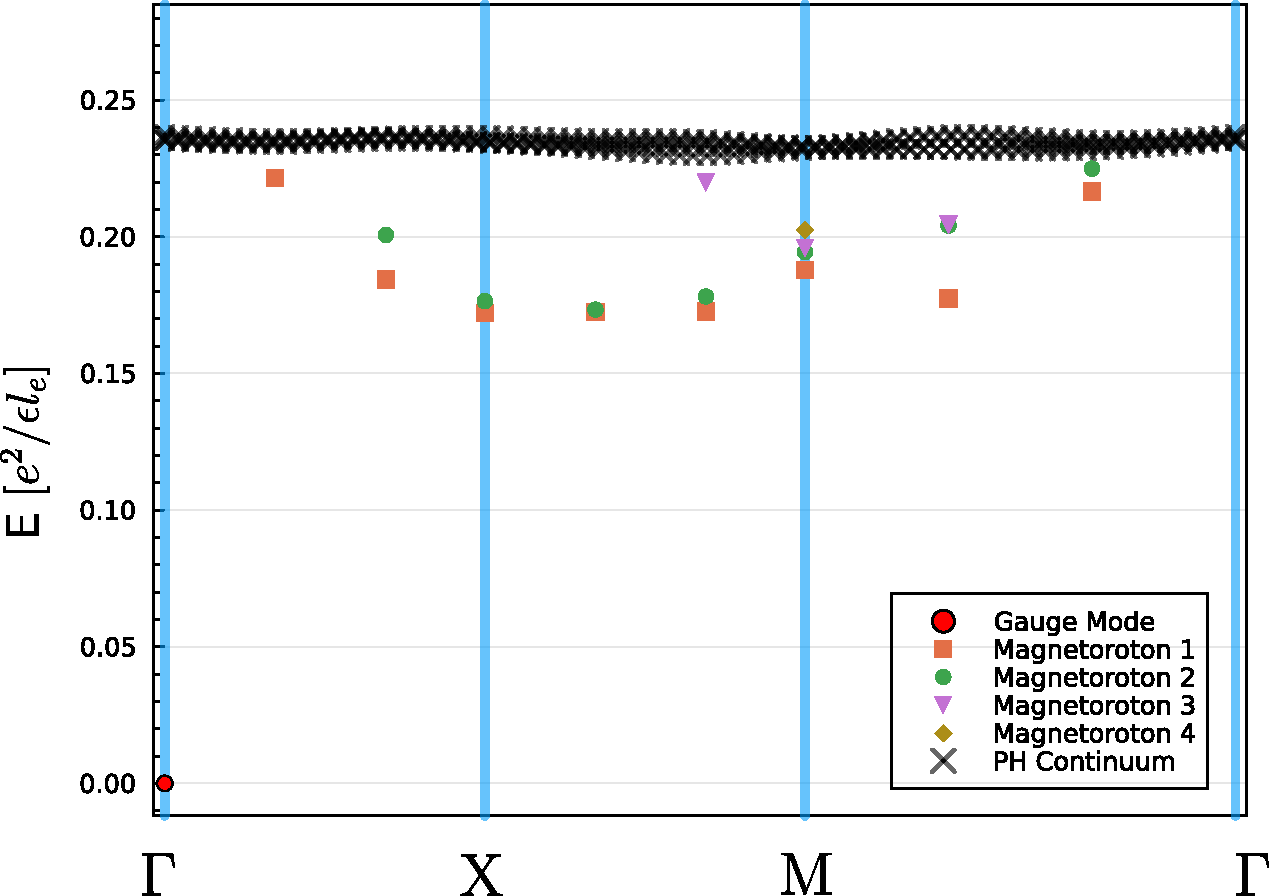
\includegraphics[width=0.95\linewidth]{figures/FCI/supplemental_tdhf_bands.pdf}
        \caption{Magnetoroton bands for the $6\times6$ MLL model.}
        \label{fig: supplemental tdhf bands}
    \end{figure}

\end{subappendices}
% \chapter{Engineering Chiral Topological Superconductivity in Twisted Ising Superconductors}

\section{Introduction}
Transition metal dichalcogenides (TMD) are van der Waals (vdW) materials and can be prepared as 2D atomic crystals. They have attracted considerable interest and have demonstrated rich electronic phenomena ranging from charge-density wave order, superconducitivity, exciton formation to the optical control of the valley degrees of freedom \cite{lian2018unveiling,he2020valley,jones2013optical,rivera2016valley,li2021optical}. Strikingly, when prepared in few-layer forms, the so-called Ising superconductors gated-2H-MoS$_2$, 2H-NbSe$_2$, 2H-TaS$_2$, 2H-NbS$_2$ and 2H-TaSe$_2$ have anomalously large in-plane upper critical field, several times beyond the Pauli limit \cite{costanzo2016gate,yan2019thickness,Cho2021,de2018tuning,li2017superconducting,lian2019coexistence}. The physical reason for this behavior can be attributed to strong Ising spin-orbit coupling in these materials, which pins the electrons' spin along the $z$-direction and is much less susceptible to an in-plane magnetic field.

Due to their 2D nature, TMD allow the fabrication of various vdW heterostructures with flexible tunability and interplay between electronic structures, superconductivity and magnetism. For instance, the ferromagntic proximity effect in monolayer TMD has been well characterized in heterostructures such as WSe$_2$/CrI$_3$ \cite{cai2019atomically,aivazian2015magnetic,mcguire2017magnetic} via optical probes. More recently, ferromagnetic Josephson junction NbSe$_2$/Cr$_2$Ge$_2$Te$_6$/NbSe$_2$ have been fabricated and investigated, and unconventional Josephson phase is reported \cite{ai2021van,idzuchi2020van}.

On the other hand, a new paradigm in the engineering of quantum phases of matter has been recently developed based on moir\'{e} patterns \cite{cao2018correlated,cao2018unconventional,bistritzer2011moire} introduced by stacking 2D crystals with twisting angles. Motivated by the discovery of correlated insulators and superconductivity in twisted bilayer graphene, the idea of moir\'{e} engineering has been extended into other materials including TMD \cite{li2021imaging,devakul2021magic,angeli2021gamma,wu2019topological}.

Interestingly, recent theories pointed out that twisted bilayer cuprate (Bi2212) may realize chiral topological superconductivity with nonzero Chern numbers \cite{can2021high,song2021doping,zhao2021emergent} --- a novel state of matter that yet to be experimentally confirmed, which has triggered further experimental and theoretical investigations \cite{volkov2020magic,volkov2021josephson}. The crucial mechanism of realizing nontrivial topology here is based on the nodal superconductivity, due to sign changes of the pairing order parameter around the Fermi surface. Intuitively, nodal superconductors are naturally located on the boundary between trivial and nontrivial band topology, and engineering topological phases via perturbations becomes possible.

In order to fabricate moir\'{e} structures, vdW 2D crystals are highly desirable. Practically, however, Bi2212 may be the only known nodal superconductor among vdW 2D crystals. This puts forward a serious constraint on the moir\'{e}-engineering of topological superconductivity. For example, the TMD superconductors are known to be nodeless and s-wave superconductors, despite theoretical discussions on the role played by magnetic fluctuations in the pairing mechanism \cite{shaffer2020crystalline}. It would be unfortunate if they cannot be included in the moir\'{e}-engineering of topological superconductivity, especially considering their fabricational flexibililty and tunability.

Motivated by these experimental and theoretical efforts, we ask the following question: is it possible to moir\'{e}-engineer topological superconductivity in TMD superconductors? The answer is positive. We find that twisted Ising superconductors like 2H-NbSe$_2$ and 2H-TaS$_2$ in the presence of an proximity-induced in-plane Zeeman field (beyond the Pauli limit) and out-of-plane supercurrent can host chiral topological superconductivity with Chern number 12 or 6. The topological phases are found to be robust and occupies physically realizable parameter regimes. Under proper experimental conditions the topological pairing gap is $>0.1$meV.

Not surprisingly, the mechanism underlying our proposal still involves pairing-gap-closing nodes, required by a trivial-to-topological phase transition. Here the pairing nodes are induced by the in-plane Zeeman field (beyond the Pauli limit) for Ising superconductors with Fermi pockets around the $\Gamma$-point in the momentum space. These Zeeman-field induced nodes were firstly pointed out theoretically by He et.al. \cite{he2018magnetic}, and experimental evidences for such nodal states in the presence of an external magnetic field have been reported \cite{xi2016ising,xing2017ising,de2018tuning,navarro2016enhanced}.

Unlike the proposal based on cuprates \cite{can2021high,song2021doping}, here the topological superconductivity in TMD twisted bilayers is limited to low temperatures $\lesssim 1$K. Nevertheless, it is worth mentioning a few advantages of the present proposal. First, different from strongly-correlated cuprates, the TMD Ising superconductivity has been fairly well-understood as conventional s-wave pairing without strong correlations. Namely the low energy physics of TMD are well under control in terms of theoretical modelling. Second, detecting the chiral majorana edge modes is the smoking-gun experiment to identify chiral topological superconductivity. In the present proposal, these edge modes are sharply located at the edge of the ferromagnetic buffer layer, and can be detected using either thermal transport or scanning tunnelling microscope (STM) (see FIG.\ref{fig: proposals} for an illustration). In the proposal based on cuprates, these edge modes will hybridize with the nodal superconductivity due to the irregular shape of the atomically thin flakes, and could be challenging to locate in real space.


\section{Main results}
Unlike twisted bilayer graphene, twisted heterostructures of TMDs have two distinct configurations differ by a 180$^\circ$ relative rotation, which were referred to as $\alpha$ and $\beta$  \cite{xian2019multiflat}. The $\alpha$-bilayer can be viewed as the building block for the bulk 2H-TMD structure, which restores the inversion symmetry. In this paper we instead focus on $\beta$-bilayer structure of Ising superconductors with Fermi pockets around the $\Gamma$-point (e.g. 2H-NbSe$_2$, 2H-TaS$_2$ but not gated 2H-MoS$_2$). In addition, a ferromagnetic insulating buffer layer with an in-plane magnetic moment is placed in the middle of the $\beta$-bilayer. At small twisting angles between the top and bottom TMD monolayers, we show that the system hosts chiral topological superconductivity when an out-of-plane supercurrent is present (see FIG.\ref{fig: proposals} for an illustration).
\begin{figure*}
	\centering
	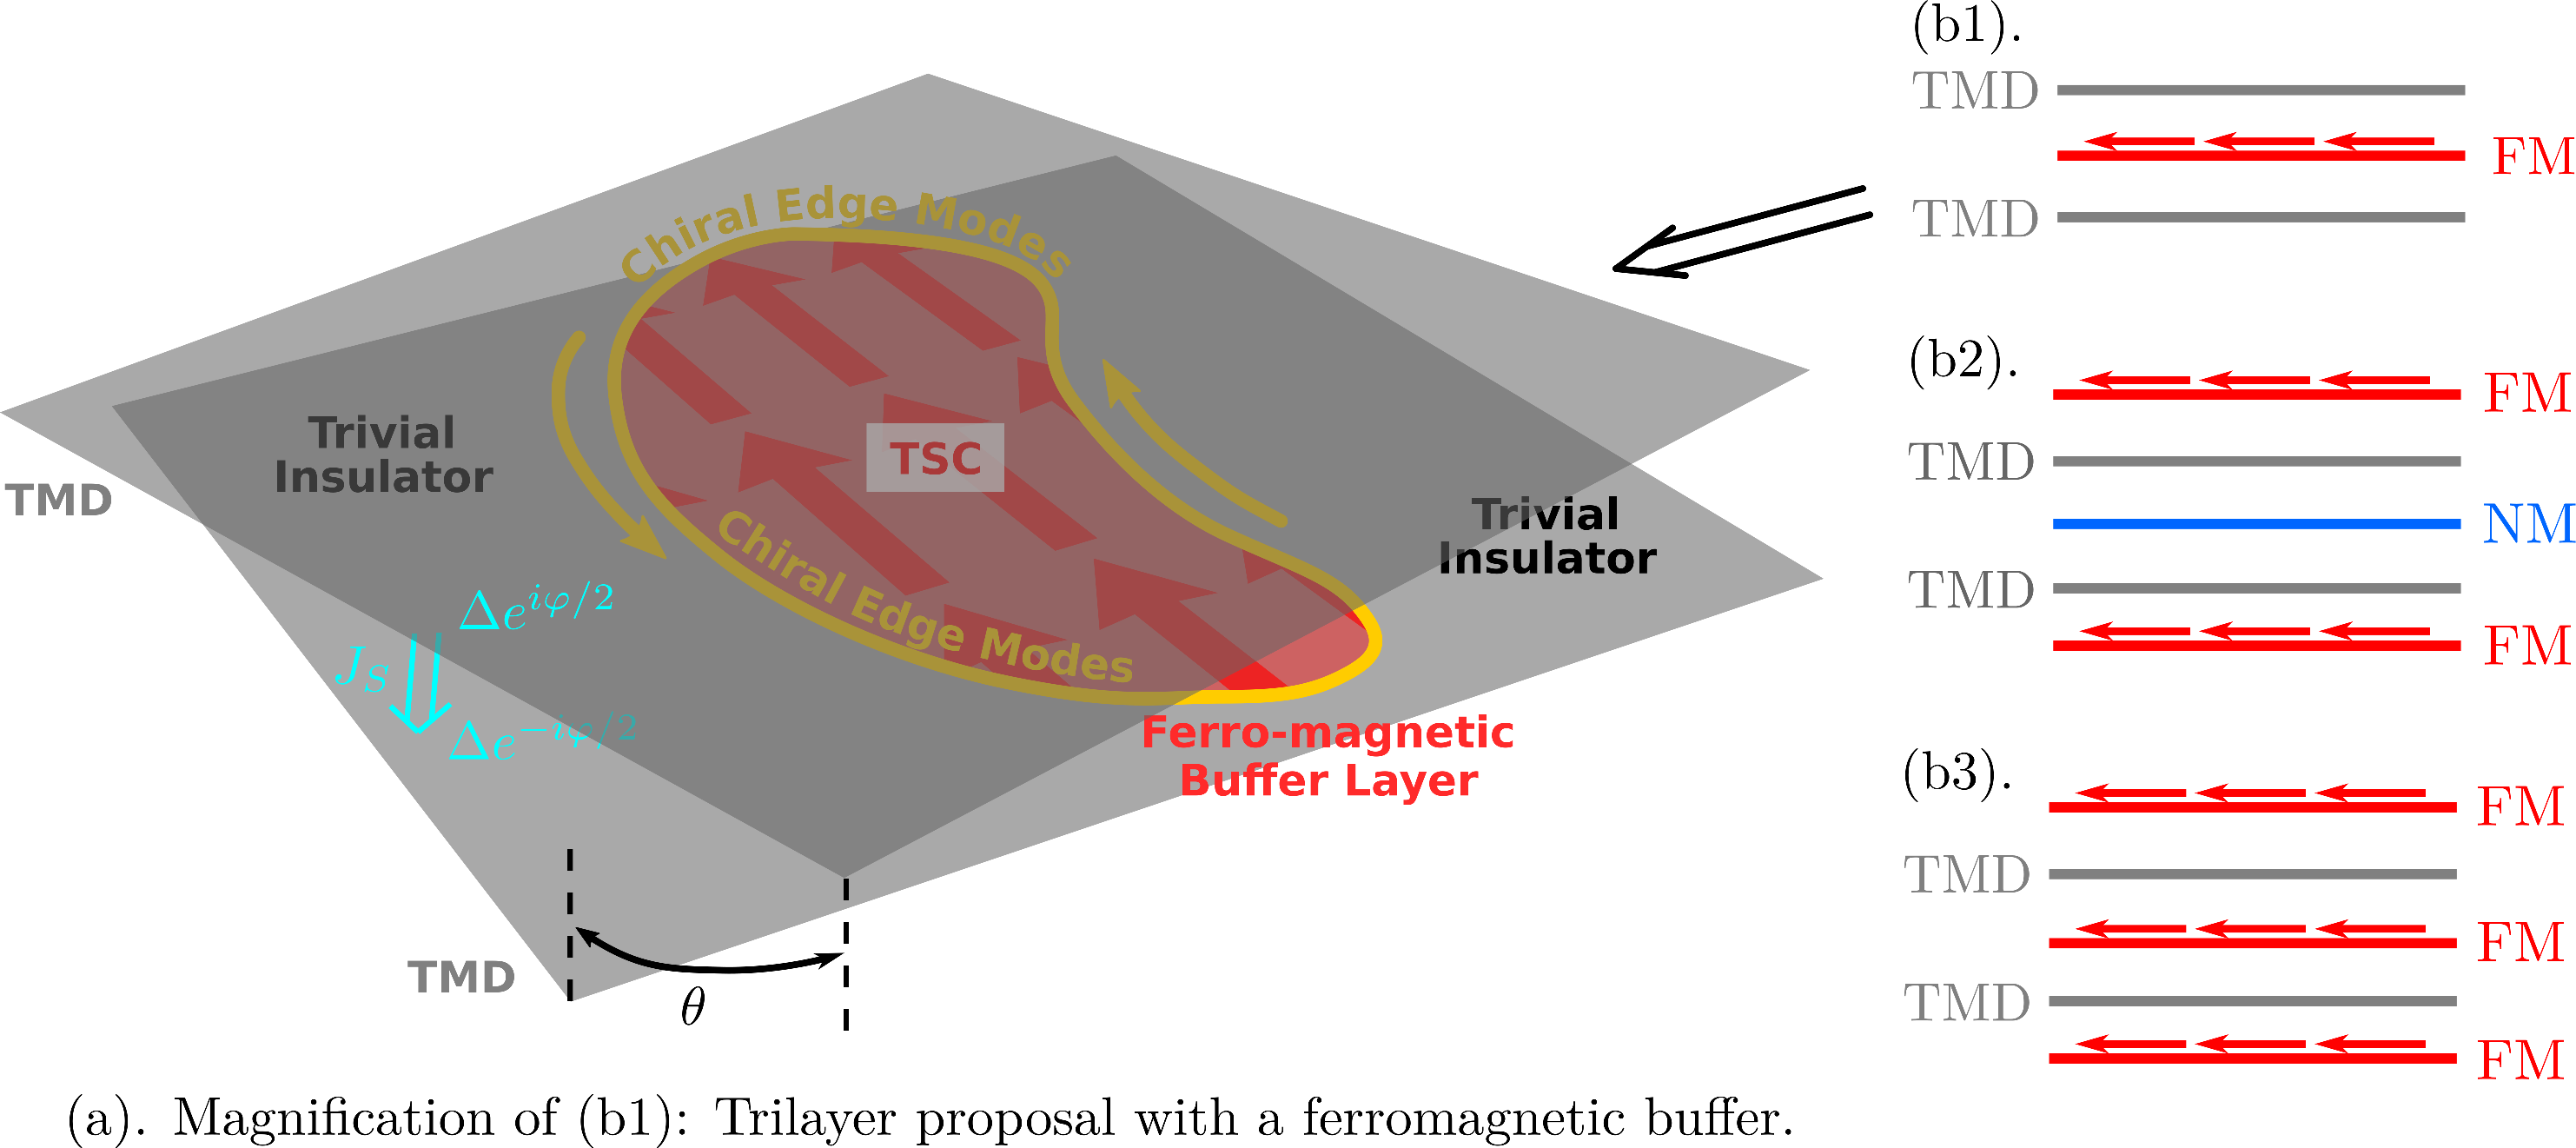
\includegraphics[width=1.0\textwidth]{contents/Ising_Top/figures/pdf_files/Magnetic_Buffer_Layer.combo.pdf}
	\caption{{\bf Setups}: Proposals of twisted $\beta$-bilayer TMD heterostructures with an insulating middle buffer layer. (a,b1): The vertical cyan arrow represents the super-current $J_S$ tuning the Josephson phase between top and bottom layers of TMD, and $\theta$ is a small twisting angle. The middle buffer layer with an \emph{in-plane} ferromagnetic moment (red arrows)  introduces an exchange Zeeman field $H_{\text{exch.}}$ for TMD layers through magnetic proximity effect, realizing the chiral topological superconducting phase. Outside the trilayer overlapping region, trivial superconductivity is realized. The gapless chiral edge modes are localized (yellow curves and arrows) at the boundary of the overlapping region. (b2,b3): Two additional proposals in the same spirits allowing more tunabilities for the parameters $t_\perp,t_{s,\perp}$ and $H_{\text{exch.}}$: FM (NM) means a ferromagnetic (nonmagnetic) buffer layer.}
	\label{fig: proposals}
\end{figure*}

Experimentally, most ferromagnetic vdW materials have an out-of-plane magnetic anisotropy. Only recently the monolayer CrCl$_3$ has been successfully isolated and confirmed to have an in-plane ferromagnetic order \cite{cai2019atomically,lu2020meron}. On the other hand, theoretical first-principle calculations predicted that monolayer $\mathrm{Cr_2I_3Cl_3}$ \cite{zhang2020electronic}, 2H-$\mathrm{VS_2}$ \cite{fuh2016newtype} and 2H-$\mathrm{VSe_2}$ \cite{zhang2019magnetic,kezilebieke2020electronic} should be insulators with in-plane ferromagnetic order. In addition, because of a weak magnetic anisotropy, the ferromagnetic moment in CrBr$_3$ can be re-oriented to an in-plane direction by a fairly small external magnetic field ($\sim 0.5$T)\cite{aikebaier2022controlling}. These vdW materials may serve as the ferromagnetic buffer layer in the present proposal.

Apart from the intrinsic electronic structures of the monolayer TMD, the proposed heterostructures are characterized by three parameters: the Zeeman exchange field $H_{\text{exch.}}$ induced by the magnetic proximity effect, the spin-independent interlayer hopping $t_\perp$, and the spin-dependent interlayer hopping $t_{s,\perp}$. These parameters depend on the choice of the buffer layer in the setup proposed in FIG.\ref{fig: proposals}(a). Moreover, one may consider more sophisticated multilayer setups as shown in FIG.\ref{fig: proposals}(b). By choosing different setups, in principle all the three parameters can be tuned individually.

In the simplest setup in FIG.\ref{fig: proposals}(a), $H_{\text{exch.}}$ and $t_{s,\perp}$ both are originated from the ferromagnetic buffer layer. In general there is no direct relation between them. However, in a mean-field treatment, the second-order perturbation theory gives $t_{s,\perp}=\mu_B H_{\text{exch.}}$ (see Appendix \ref{app:magnetic_buffer_layer_perturbation}). Although there is no available experimental data to quantify $H_{\text{exch.}}$ for the proposed heterostructures, similar heterostructures like WSe$_2$/CrI$_3$, MoSe$_2$/CrBr$_3$ with out-of-plane ferromagnetic layer have been well characterized experimentally and theoretically \cite{zhong2017van,zhong2020layer,seyler2018valley,zollner2019proximity,ciorciaro2020observation,aikebaier2022controlling}, where a proximity-induced Zeeman splitting around $1\sim2$meV is reported for electronic bands near the $K$ point. A similar value of splitting in the proposed heterostructures corresponds to $H_{\text{exch.}}=3\sim6 H_p$. Notice that monolayer NbSe$_2$ has been reported to sustain a in-plane upper critical field $6\sim 8  H_p$ \cite{xi2016ising,xing2017ising,de2018tuning} (and about $9\sim10 H_p$ for TaS$_2$ \cite{navarro2016enhanced,pan2017enhanced}).

We find that the topological phase is robust at least when a small twisting angle $\theta$ is comparable with $t_\perp/(\hbar v_{\text{Ising}} k_F)$, where $k_F$ is the Fermi wavevector and the velocity $v_{\text{Ising}}$ is characterizing the Ising spin-orbit coupling near the $\Gamma$-$M$ direction (see Eq.(\ref{eqn:1layer})). It is convenient to introduce a dimensionless parameter to capture the ratio of the two quantities:
\begin{align}
	\xi\equiv \arctan \frac{2t_\perp}{\hbar v_{\text{Ising}} k_F\theta}.\label{eqn:xi}
\end{align}

We consider proposed heterostructures involving either TaS$_2$ or NbSe$_2$. Their monolayer electronic structures are obtained using relaxed crystal structure based on first-principle calculations (see Appendix \ref{app:phase_diagram_details} for details). For each TMD material, two cases for the spin-dependent hopping $t_{s,\perp}$ are investigated, corresponding to:

\begin{align}
	\textbf{case-(i): }  & t_{s,\perp}=\mu_BH_{\text{exch.}}\notag \\
	\textbf{case-(ii): } & t_{s,\perp}=0\label{eqn:cases}
\end{align}


We show the global phase diagram by tuning the spin-independent hopping $t_\perp$ and the Zeeman exchange field $H_{\text{exch.}}$ in FIG.\ref{fig:t-H phase digram}, based on numerical calculations. For presentation purpose, we have fixed $\xi^{\mathrm{TaS_2}}=0.9$ and $\xi^{\mathrm{NbSe_2}}=1.1$, and fixed the Josephson phase $\varphi=\pi/2$ corresponding the maximal supercurrent state. Topological superconducting phases are found to exist when $t_\perp\lesssim 9$meV for TaS$_2$ (and $t_\perp\lesssim 2.7$meV for NbSe$_2$). A Chern-number-12 phase is found to occupy a large portion of the parameter space, while a Chern-number-6 phase appears for case-(i) at small values of $t_\perp$. Under appropriate conditions, the gap in the topological phase can reach $0.1$meV.

These phase diagrams are also well-understood via analytical calculations. We have plotted the phase boundary (see Eq.(\ref{Phase boundary})) between trivial and topological phases from our perturbative calculations in FIG.\ref{fig:t-H phase digram}, which is in good agreement with the numerical calculations.
\begin{figure*}[!htp]
	\centering
	\begin{minipage}{1.0\textwidth}
		\RaggedRight (a). $\mathbf{TaS_2:}$\\[0.5em]
		\begin{minipage}{0.45\textwidth}
			\centering
			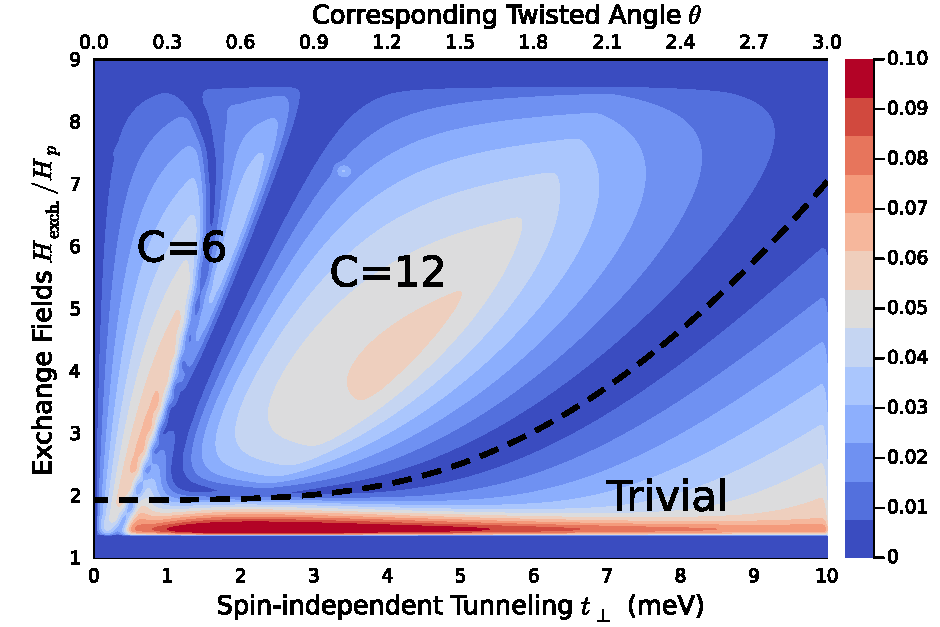
\includegraphics[width=\linewidth]{contents/Ising_Top/figures/pdf_files/Gap_Size_Phase_Diagram.TaS2.t_H.magnetic_with_prediction.pdf}\\
			case (i).
		\end{minipage}
		\hspace{1em}
		\begin{minipage}{0.45\textwidth}
			\centering
			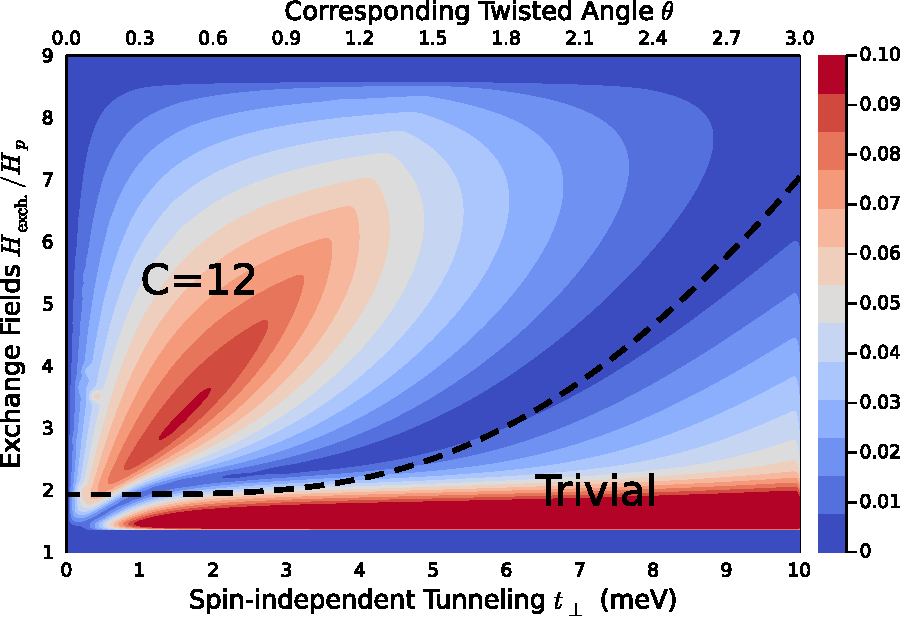
\includegraphics[width=\linewidth]{contents/Ising_Top/figures/pdf_files/Gap_Size_Phase_Diagram.TaS2.t_H.non-magnetic_with_prediction.pdf}\\
			case (ii).\\
		\end{minipage}
	\end{minipage}
	\\[1em]
	\begin{minipage}{1.0\textwidth}
		\RaggedRight (b). $\mathbf{NbSe2_2:}$\\[0.5em]
		\begin{minipage}{0.45\textwidth}
			\centering
			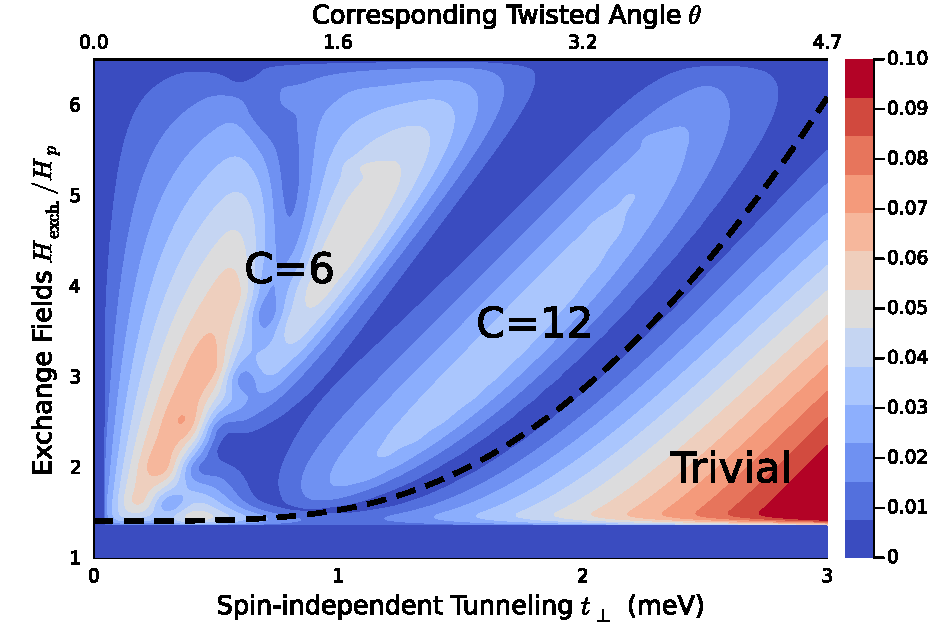
\includegraphics[width=\linewidth]{contents/Ising_Top/figures/pdf_files/Gap_Size_Phase_Diagram.NbSe2.t_H.magnetic_with_prediction.pdf}\\
			case (i).
		\end{minipage}
		\hspace{1em}
		\begin{minipage}{0.45\textwidth}
			\centering
			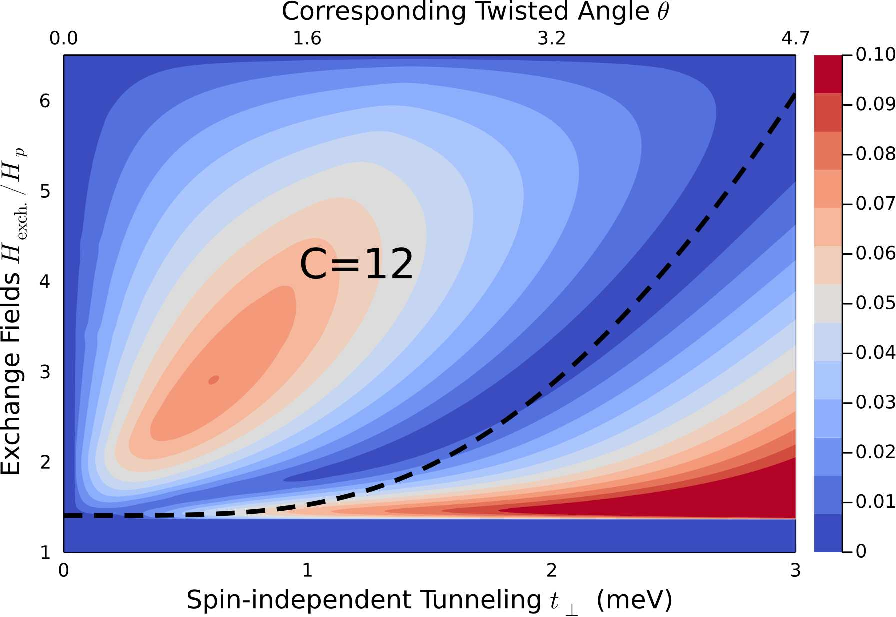
\includegraphics[width=\linewidth]{contents/Ising_Top/figures/pdf_files/Gap_Size_Phase_Diagram.NbSe2.t_H.non-magnetic_with_prediction.pdf}\\
			case (ii).\\
		\end{minipage}
	\end{minipage}
	%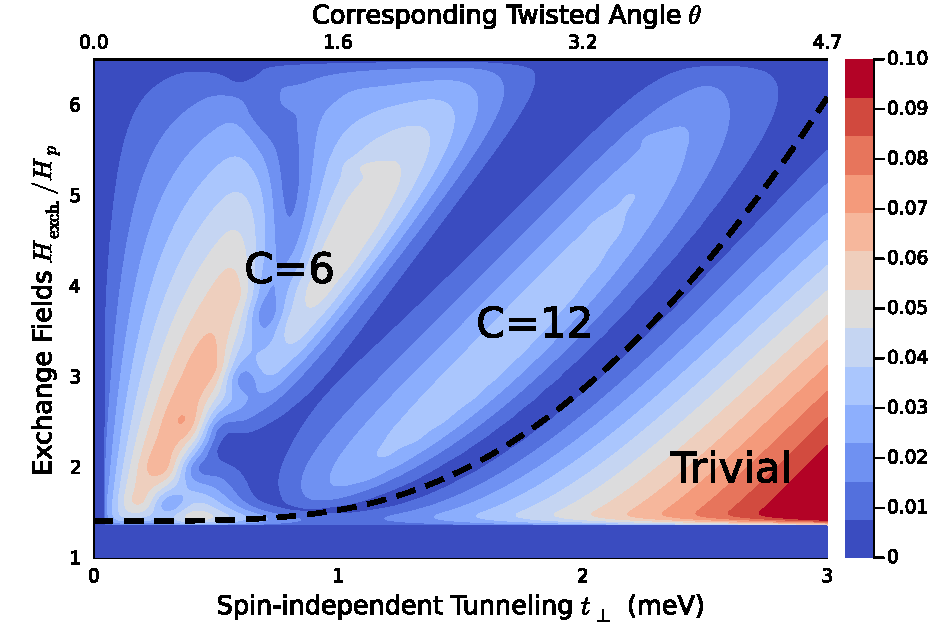
\includegraphics[scale=0.5]{contents/Ising_Top/figures/pdf_files/Gap_Size_Phase_Diagram.NbSe2.t_H.magnetic_with_prediction.pdf}
	%\hspace{1em}
	%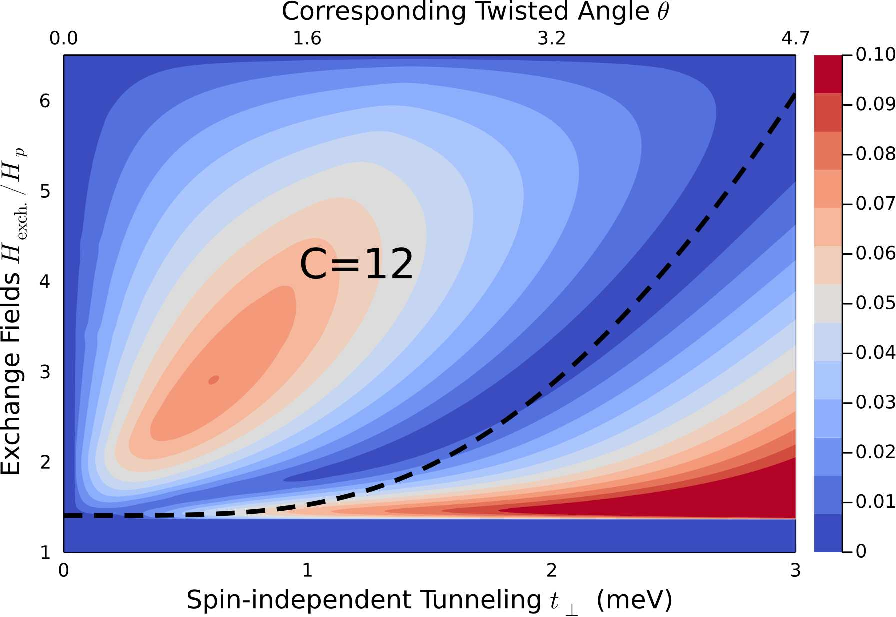
\includegraphics[scale=0.5]{contents/Ising_Top/figures/pdf_files/Gap_Size_Phase_Diagram.NbSe2.t_H.non-magnetic_with_prediction.pdf}
	\caption{{\bf $t_\perp$-$(H/H_p)$ Phase Diagram:} The superconducting gap (gap minimum in the momentum space) and Chern numbers for proposed heterostructures involving $\mathrm{TaS_2}$ (a) and $\mathrm{NbSe_2}$ (b) based on numerical calculations. Here the Josephson phase is fixed to be $\varphi=\pi/2$ and the parameter $\xi$ (see Eq.(\ref{eqn:xi}) for its definition) is fixed to be $\xi^{\mathrm{TaS_2}}=0.9$ and $\xi^{\mathrm{NbSe_2}}=1.1$. $H_p$ in the vertical axis is the Pauli limit field strength. $t_\perp$ and the corresponding twisting angle are displayed on the horizontal axis. For both materials the phase diagrams corresponding to case-(i) and case-(ii) in Eq.(\ref{eqn:cases}) are calculated. The black dashed lines exhibit the predicted topological/trivial phase boundary from analytical perturbative calculations (see Eq.(\ref{Phase boundary})).}
	\label{fig:t-H phase digram}
\end{figure*}


Apart from the global phase diagrams, we also plot the phase diagrams with a few selected values of $t_\perp$. Fixing $H_{\text{exch.}}=4H_p$, we tune the twisting angle $\theta$ and the Josephson phase $\varphi$, and the results are shown in FIG.\ref{fig:theta-phi phase digram}. Consistent with the global phase diagram, the topological phase is realized when $t_\perp$ is not too large. Interestingly, for intermediate values of $t_\perp$, trivial to topological phase transitions are observed by tuning $\varphi$ alone while fixing the twisting angle $\theta$ in an appropriate regime. Such a Josephson-phase-driven topological transition in a single device can lead to unique features to unambiguously identify the topological phase in experiments. For instance, the gapless chiral majorana edge modes should appear only in the topological phase, after the phase transition occurs when $\varphi$ is tuned up.
\begin{figure*}
	\raggedright(a). $\mathbf{TaS_2:}$\\[1em]
	\begin{minipage}{1.0\textwidth}
		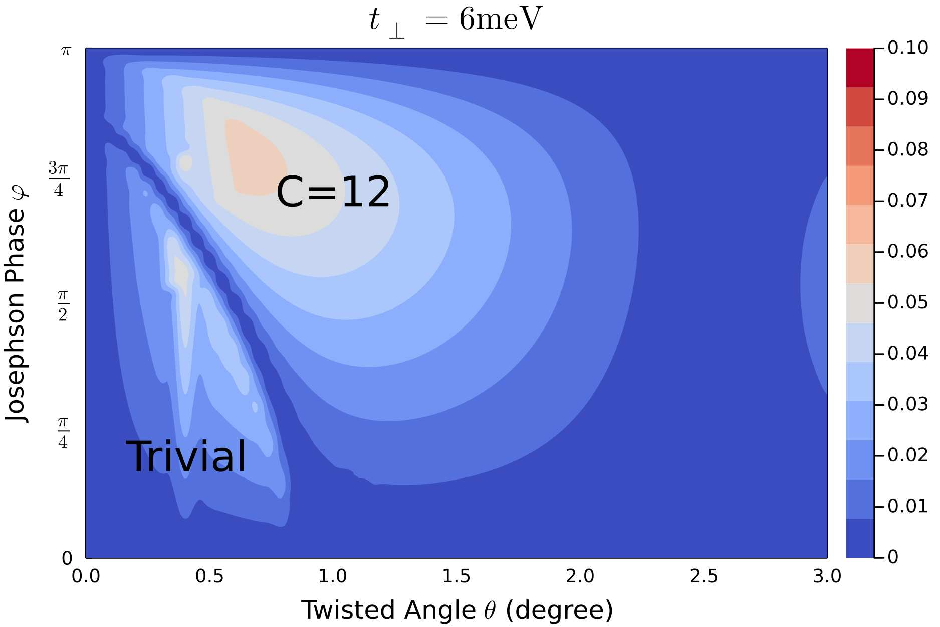
\includegraphics[width=0.33\linewidth]{contents/Ising_Top/figures/pdf_files/gap_size_distribution.TaS2.theta_phi.magnetic.t=6.pdf}
		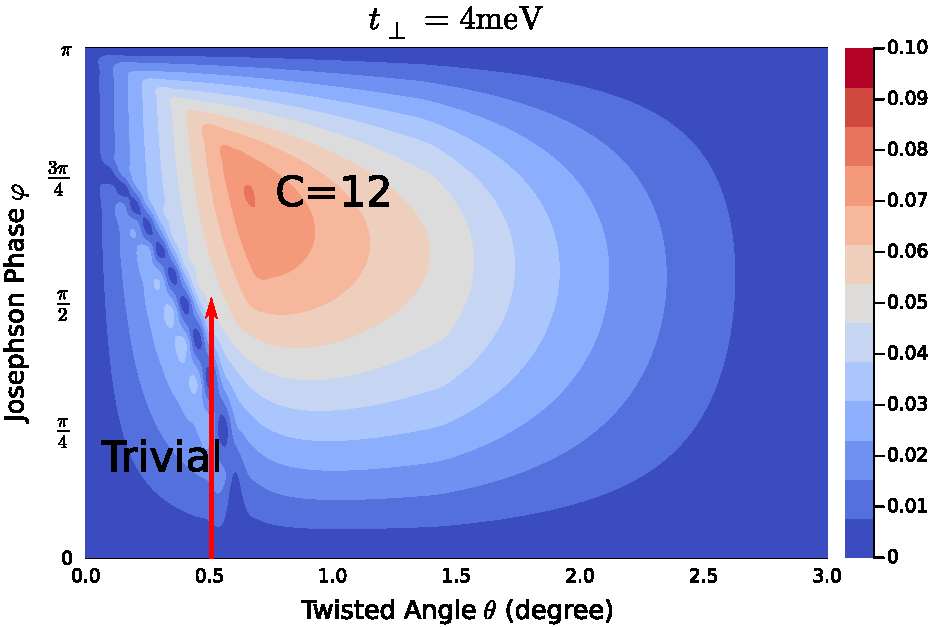
\includegraphics[width=0.33\linewidth]{contents/Ising_Top/figures/pdf_files/gap_size_distribution.TaS2.theta_phi.magnetic.t=4.pdf}
		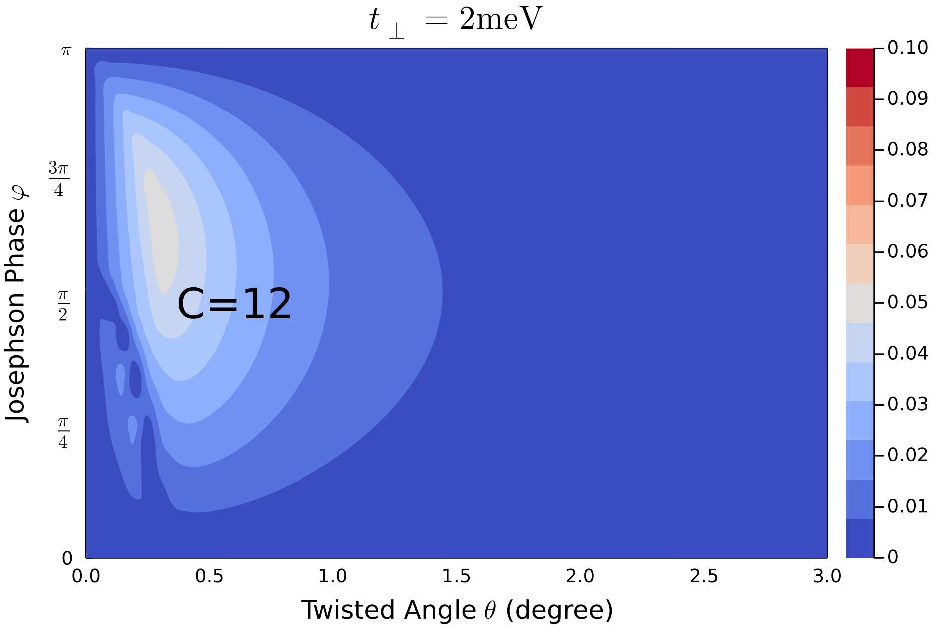
\includegraphics[width=0.33\linewidth]{contents/Ising_Top/figures/pdf_files/gap_size_distribution.TaS2.theta_phi.magnetic.t=2.pdf}
		\\
		case (i)\\[1em]
		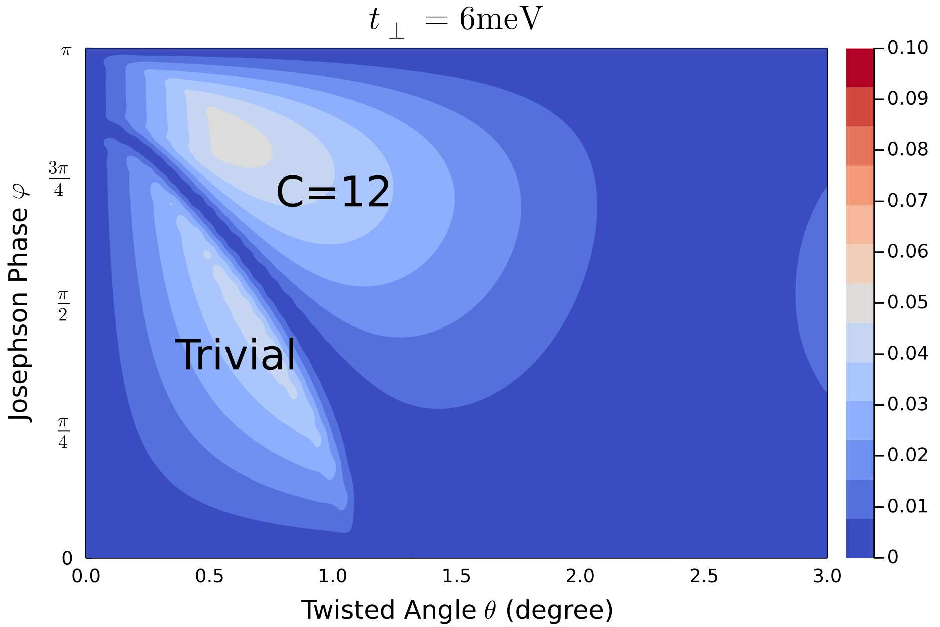
\includegraphics[width=0.33\linewidth]{contents/Ising_Top/figures/pdf_files/gap_size_distribution.TaS2.theta_phi.non-magnetic.t=6.pdf}
		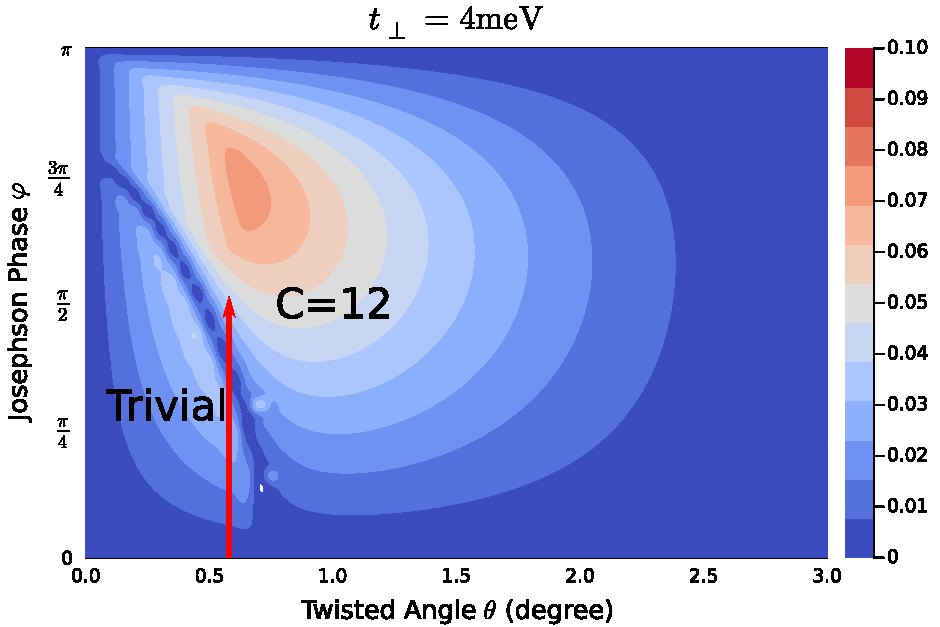
\includegraphics[width=0.33\linewidth]{contents/Ising_Top/figures/pdf_files/gap_size_distribution.TaS2.theta_phi.non-magnetic.t=4.pdf}
		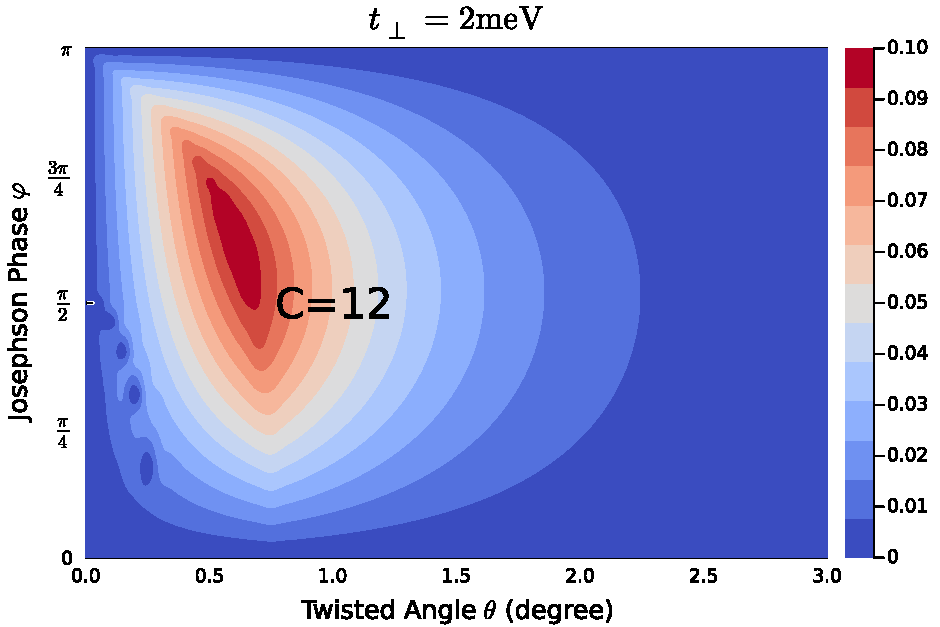
\includegraphics[width=0.33\linewidth]{contents/Ising_Top/figures/pdf_files/gap_size_distribution.TaS2.theta_phi.non-magnetic.t=2.pdf}
		\\
		case (ii)
	\end{minipage}
	\\
	\vspace{1.5em}
	\raggedright(b). $\mathbf{NbSe_2:}$\\[1em]
	\begin{minipage}{1.0\textwidth}
		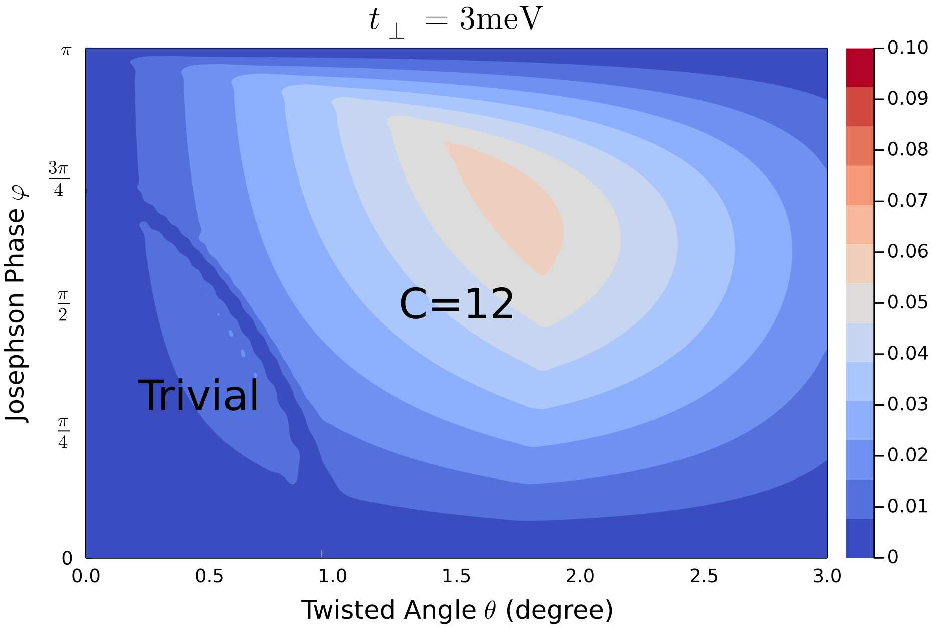
\includegraphics[width=0.33\linewidth]{contents/Ising_Top/figures/pdf_files/gap_size_distribution.NbSe2.theta_phi.magnetic.t=3.pdf}
		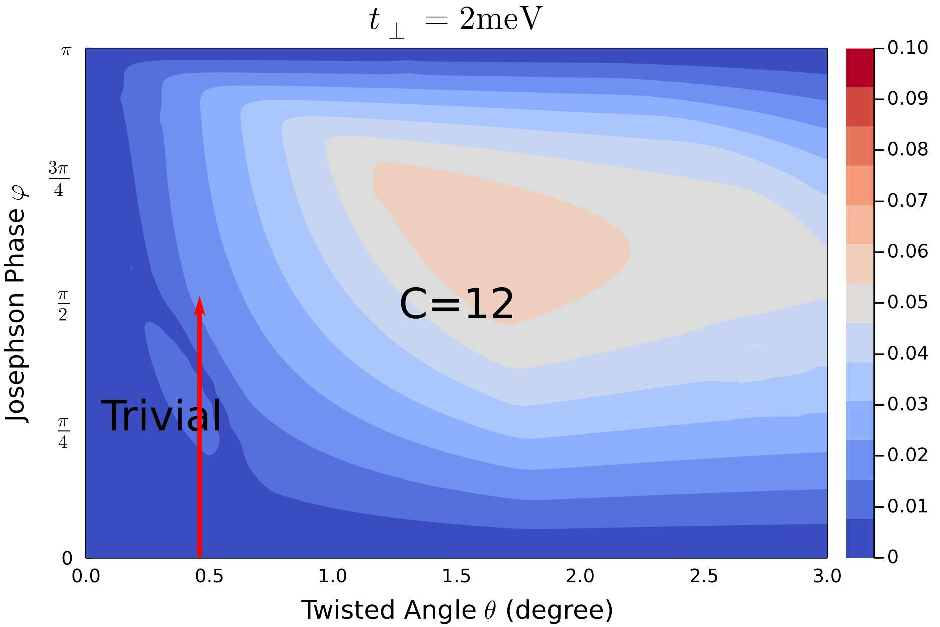
\includegraphics[width=0.33\linewidth]{contents/Ising_Top/figures/pdf_files/gap_size_distribution.NbSe2.theta_phi.magnetic.t=2.pdf}
		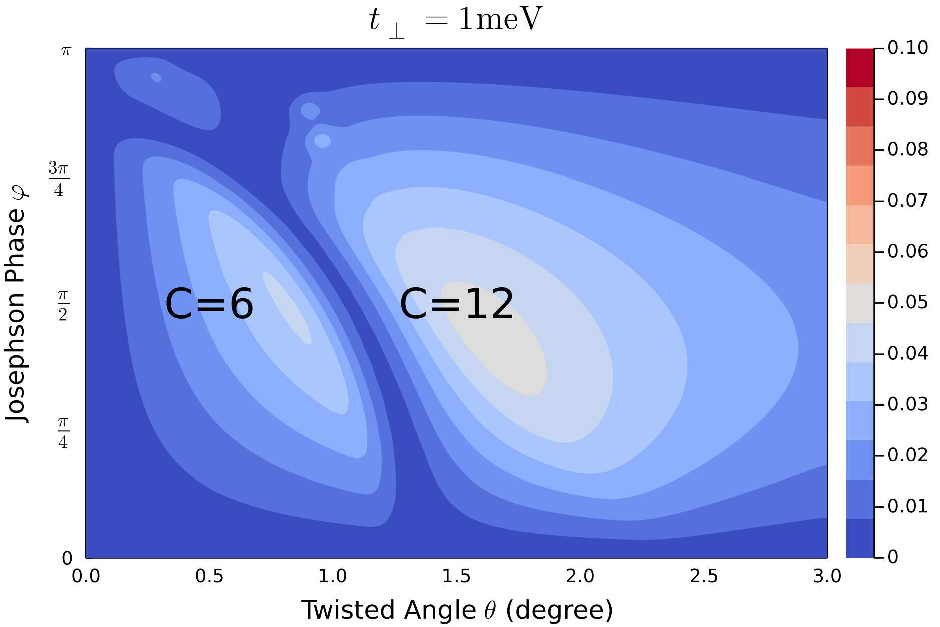
\includegraphics[width=0.33\linewidth]{contents/Ising_Top/figures/pdf_files/gap_size_distribution.NbSe2.theta_phi.magnetic.t=1.pdf}
		\\
		case (i)\\[1em]
		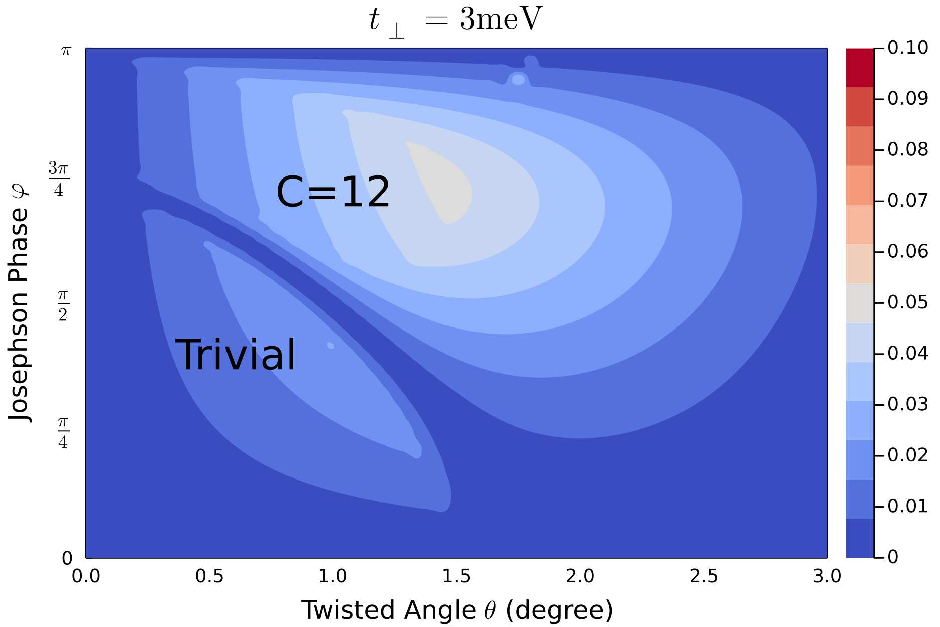
\includegraphics[width=0.33\linewidth]{contents/Ising_Top/figures/pdf_files/gap_size_distribution.NbSe2.theta_phi.non-magnetic.t=3.pdf}
		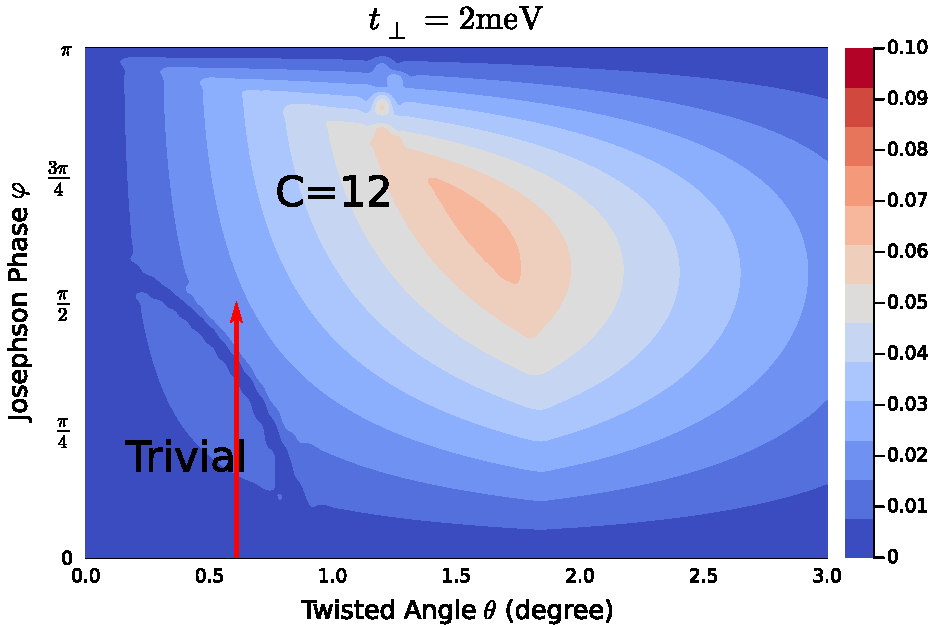
\includegraphics[width=0.33\linewidth]{contents/Ising_Top/figures/pdf_files/gap_size_distribution.NbSe2.theta_phi.non-magnetic.t=2.pdf}
		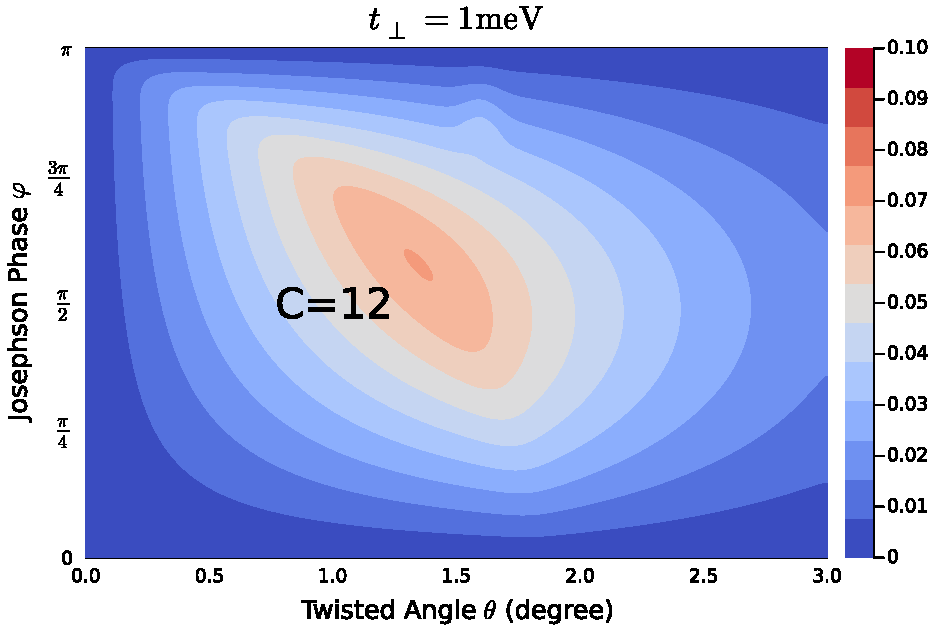
\includegraphics[width=0.33\linewidth]{contents/Ising_Top/figures/pdf_files/gap_size_distribution.NbSe2.theta_phi.non-magnetic.t=1.pdf}
		\\
		case (ii)
	\end{minipage}
	\caption{{\bf $\theta$-$\varphi$ Phase Diagram:} The superconducting gap (gap mininum in the momentum space) and Chern numbers by varying the twisting angle $\theta$ and the Josephson phase $\varphi$ for proposed heterostructures involving $\mathrm{TaS_2}$ and $\mathrm{NbSe_2}$. Here in each figure we fix the Zeeman field to be four times the Pauli limit $H_{\text{exch.}}=4H_p$ and fix the spin-independent tunneling $t_\perp$. Red arrows are to indicate the trivial-topological phase transitions by tuning $\varphi$ in a single device. Note that the regime $\varphi\leq \pi/2$ corresponds to the stable branch of the Josephson junction.}
	\label{fig:theta-phi phase digram}
\end{figure*}

\section{Model}
In an in-plane Zeeman field regime $H_{\text{exch.}}>\sqrt{2}H_p$, it was pointed out that the pairing gap around the $\Gamma$-pockets will close and nodal superconductivity is formed \cite{he2018magnetic}, while the pairing gap around the $K$-pockets remain nodeless. These nodes on $\Gamma$-pockets turn out to be the origin of the topological superconductivity in the present proposal.

The minimal model for the bands forming the $\Gamma$-pockets (which has dominant $d_{z^2}$ orbital content of the transition metal) is as follows
\begin{align}
	h(\bm k)=\varepsilon_0(\bm k)+\lambda^{\text{Ising}}_{\mathrm{SO}}(\bm k) \sigma_z.
\end{align}
Drastically different from the usual Rashba spin-orbit coupling, here the Ising spin-orbit coupling $\lambda^{\text{Ising}}_{\mathrm{SO}}(\bm k)$ splits bands with fixed $S_z$-spin. In fact, due to the $z\rightarrow -z$ mirror symmetry of monolayer 2H-TMD, the Rashba spin-orbit coupling is forbidden. Time-reversal symmetry dictates that $\lambda^{\text{Ising}}_{\mathrm{SO}}(\bm k)=-\lambda^{\text{Ising}}_{\mathrm{SO}}(-\bm k)$, so $\lambda^{\text{Ising}}_{\mathrm{SO}}(\bm k)$ necessarily has sign changes. Due to the mirror plane containing the $\Gamma$-$M$ axis, the six $\Gamma$-$M$ directions are exact where $\lambda^{\text{Ising}}_{\mathrm{SO}}(\bm k)$ changes sign.

We therefore begin with a first-order $\bm{k\cdot p}$ model near the intersection point $P$ between the Fermi surface and one $\Gamma$-$M$ direction ($k_x$-direction, see Fig.\ref{fig: monolayer FS} for an illustration):
\begin{align}
	h^{\text{mono.}}=\hbar v_F k_x + \hbar v_{\text{Ising}} k_y\sigma_z,\label{eqn:1layer}
\end{align}
where $\lambda^{\text{Ising}}_{\mathrm{SO}}(\bm k)$ vanishes along the $k_x$-direction, and $v_{\text{Ising}}\equiv \frac{\partial \lambda^{\text{Ising}}_{\mathrm{SO}}(\bm k)}{\hbar \partial k_y}$. We list these parameters for NbSe$_2$ and TaS$_2$ in Table.\ref{table:parameters} based on first principle calculations (Fig. \ref{fig: band_plot Gamma-M-K} plot the band structures, full list of quartic $\bm{k\cdot p}$ expansion parameters is given in Appendix \ref{app:phase_diagram_details}).
\begin{table}
	\centering
	\begin{tabular}{|c|c|c|c|c|}
		\hline
		TMD      & $\hbar v_F$(eV$\cdot$\AA) & $\hbar v_{\text{Ising}}$ (eV$\cdot$\AA) & $k_F$ (\AA$^{-1}$) & $\Delta$ (meV) \\ \hline
		NbSe$_2$ & -2.22                     & 0.12                                    & 0.48               & 0.46           \\ \hline
		TaS$_2$  & -2.89                     & 0.36                                    & 0.54               & 0.52           \\ \hline
	\end{tabular}
	\caption{The parameters in the $\bm{k\cdot p}$ model.}
	\label{table:parameters}
\end{table}

\vspace{1em}
\textbf{Monolayer:} After introducing an spin-singlet pairing $\Delta$ \footnote{$\Gamma$-$M$ mirror symmetry protects that there is no singlet-triplet mixing at $P$-point.}, in the Nambu basis we obtain the BCS mean-field Hamiltonian:
\begin{align}\label{eqn:1layer_bcs}
	h^{\text{mono.}}_{\text{BCS}}= & \hbar v_F k_x \tau_z+ \hbar v_{\text{Ising}} k_y\sigma_z+\mu_B H_y \sigma_y+\Delta \sigma_y\tau_y,
\end{align}
where Pauli $\tau$-matrices label the particle-hole space, and an Zeeman field $H_y$ along the $y$-direction is introduced (the g-factor is assumed to be 2). Because the system has a spin-rotation symmetry around $S_z$-direction, the choice of the direction of the in-plane magnetic field is not important. Since there are three independent $\Gamma$-$M$-directions, related by $C_3$ rotations, the full electronic structure of NbSe$_2$ (TaS$_2$) has three copies of the effective theory in Eq.(\ref{eqn:1layer_bcs}).
\begin{figure*}
	\centering
	\raisebox{-0.5\height}{
		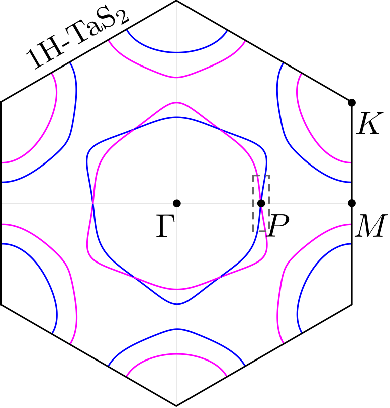
\includegraphics[scale=0.75]{contents/Ising_Top/figures/pdf_files/monolayer_Fermi_Surface_TaS2.pdf}
	}
	\hspace{1.5em}
	\raisebox{-0.5\height}{
		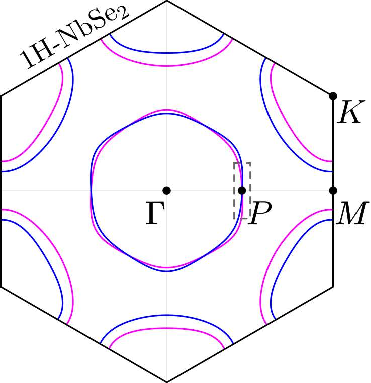
\includegraphics[scale=0.75]{contents/Ising_Top/figures/pdf_files/monolayer_Fermi_Surface_NbSe2.pdf}
	}
	\raisebox{-0.5\height}{
	$\xymatrix @+2em { \ar@{=>}[r]^{\text{\small Magnify}}_{\text{\small Dash box}} & }$
	}
	\raisebox{-0.5\height}{
		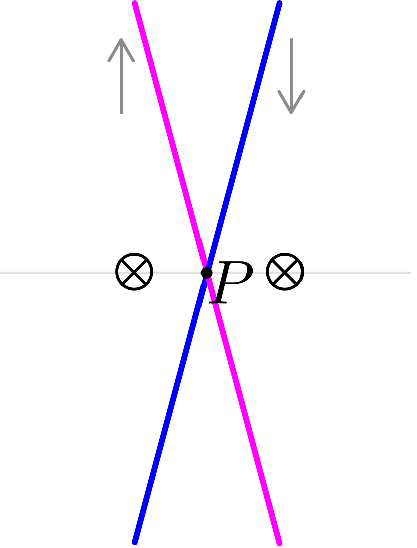
\includegraphics[scale=0.4]{contents/Ising_Top/figures/pdf_files/node.pdf}
	}
	\caption{{\bf Monolayer Fermi Surfaces and Band Structures:} $\Gamma$-pocket and $K$-pocket of monolayer $\mathrm{NbSe_2}$ and $\mathrm{TaS_2}$ are shown. Point $P$ is the intersection of $\Gamma$-$M$ line and the the $\Gamma$-pocket, where Ising SOC vanishes and two nodes (cross symbols) emerge when an in-plane Zeeman field $H_{\text{exch.}}$ exceeds the superconducting gap. Magenta and blue colors indicate the different $S_z$-spin components.}
	\label{fig: monolayer FS}
\end{figure*}
Eq.(\ref{eqn:1layer_bcs}) can be solved straightforwardly. A pair of Dirac nodes are found to emerge when $\mu_B H_y>\Delta$, located at $\bm k^{\pm}=(\pm \frac{1}{\hbar v_F} \sqrt{(\mu_B H_y)^2-\Delta^2},0)$ (see Fig.\ref{fig: monolayer FS}) for a schematic illustration, consistent with earlier works \cite{he2018magnetic,shaffer2020crystalline}, whose low energy effective theories are:
\begin{align}
	h^{\pm}_{\text{node}}=\pm\hbar v_F \cos\eta \delta k_x\Sigma_z+\hbar v_{\text{Ising}}\sin\eta \delta k_y\Sigma_x,\label{eqn:1layer_eff}
\end{align}
where $\eta=\arcsin\frac{\Delta}{\mu_B H_y}$, $\delta \bm k$ is measured from the nodal points $\bm k^{\pm}$, and $\Sigma$ are Pauli matrices in the low energy space. These nodes are protected by a chiral symmetry $\sigma_x\tau_y$ in model Eq.(\ref{eqn:1layer_bcs}) (corresponding to the combination of the physical time-reversal transformation $i\sigma_yK$, the particle-hole transformation $\tau_x K$ and a $S_z$-$\pi$ rotation $i\sigma_z\tau_z$) sending $h(\bm k)\rightarrow -h(\bm k)$.
\begin{figure}[!htp]
	\centering
	\begin{minipage}{0.9\linewidth}
		\RaggedRight (a). $\mathbf{TaS_2}$:\\[0.5em]
		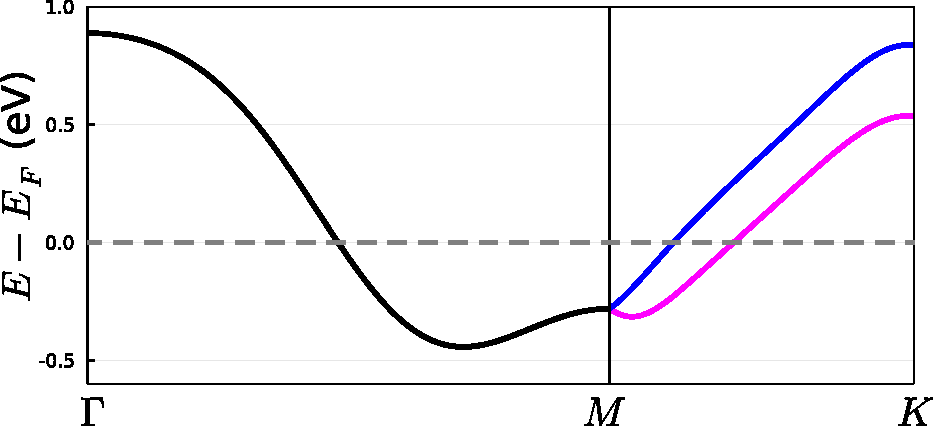
\includegraphics[width=\textwidth]{contents/Ising_Top/figures/pdf_files/monolayer_band_Gamma_M_K_TaS2.pdf}
	\end{minipage}
	\\[2em]
	\begin{minipage}{0.9\linewidth}
		\RaggedRight (b). $\mathbf{NbSe2_2}$:\\[0.5em]
		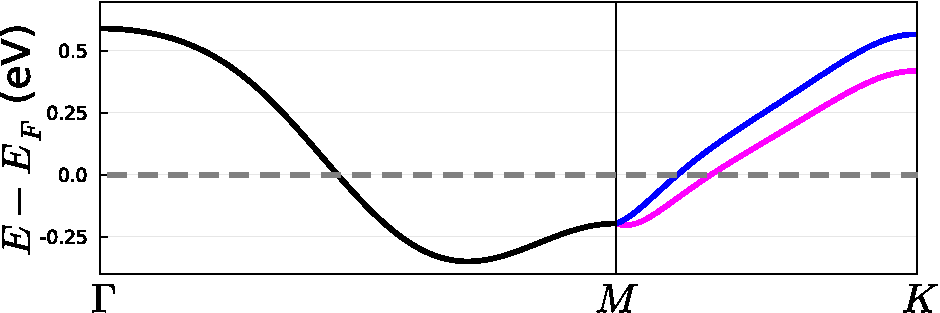
\includegraphics[width=\textwidth]{contents/Ising_Top/figures/pdf_files/monolayer_band_Gamma_M_K_NbSe2.pdf}
	\end{minipage}
	\caption{{\bf Monolayer Band Structures.}}
	\label{fig: band_plot Gamma-M-K}
\end{figure}
\vspace{1em}\par
\textbf{Twisted bilayer:} Next we consider a $\beta$-bilayer (separated by an insulator buffer layer) with a twisting angle $\theta$, which can be viewed as top/bottom monolayer twisted by angle $\pm\theta/2$ respectively. Introducing $k_F$ being the crystal momentum of point $P$, we obtain the following effective theory near $P$:
\begin{align}
	h^{\text{bilayer}}_{\text{BCS}}= & \hbar v_F k_x\tau_z+\hbar v_{\text{Ising}} k_y\sigma_z+\Delta\cos\frac{\varphi}{2}\sigma_y\tau_y\notag                         \\
	+                                & \Delta\sin\frac{\varphi}{2} \sigma_y\tau_x\nu_z-\hbar v_{\text{Ising}}k_F\frac{\theta}{2}\sigma_z\nu_z+\mu_B H_y\sigma_y\notag \\
	+                                & t_\perp \tau_z\nu_x+t_{s_y,\perp}\sigma_y\nu_x.\label{eqn:bilayer_bcs}
\end{align}
Here the Pauli matrices $\nu$ captures the top/bottom layer space. $\Delta>0$ and the pairing amplitude is $\Delta e^{\pm i\varphi/2}$ for the top/bottom layer respectively. The $t_\perp$ and $t_{s_y,\perp}$ terms describes the spin-independent and spin-dependent interlayer hopping processes respectively. Based on the two-center approximation \cite{bistritzer2011moire,devakul2021magic}, and the fact that point $P$ is far away from the Brillouin zone boundary, the interlayer hopping processes have a weak stacking-dependence, and are considered as constants in the present work \cite{volkov2020magic,volkov2021josephson} (see Appendix \ref{app:two-center approximation} for a discussion on the two-center approximation).


The model Eq.(\ref{eqn:bilayer_bcs}) can be analytically solved in various perturbative regimes. To demonstrate the stability of the topological superconductivity, below we focus on one particular regime, in which $\sqrt{(\hbar v_{\text{Ising}} k_F\theta)^2+4t_\perp^2}\gg \Delta,\mu_B H_y, t_{s_y,\perp}$. The advantage of this regime is that it is always realizable in the proposed heterostructures by tuning the twisting angle $\theta$. In this regime, we find that the topological superconductivity with Chern number 4 (corresponding to Chern number 12 for the whole heterostructure) is always realized in model Eq.(\ref{eqn:bilayer_bcs}) by tuning $\varphi,\theta$ and $\mu_B H_y \gtrsim  \Delta$.

To understand this behavior, we may firstly turn off the pairing $\Delta$ and $\mu_B H_y, t_{s_y,\perp}$  in model Eq.(\ref{eqn:bilayer_bcs}). There are four intersection points between the spin-up and spin-down Fermi surfaces, which we label as $C,D$ and $F,G$ and are located at the $k_y$ and $k_x$ axes respectively (see FIG. \ref{fig: all eight nodes}).
\begin{figure}[!htp]
	\centering
	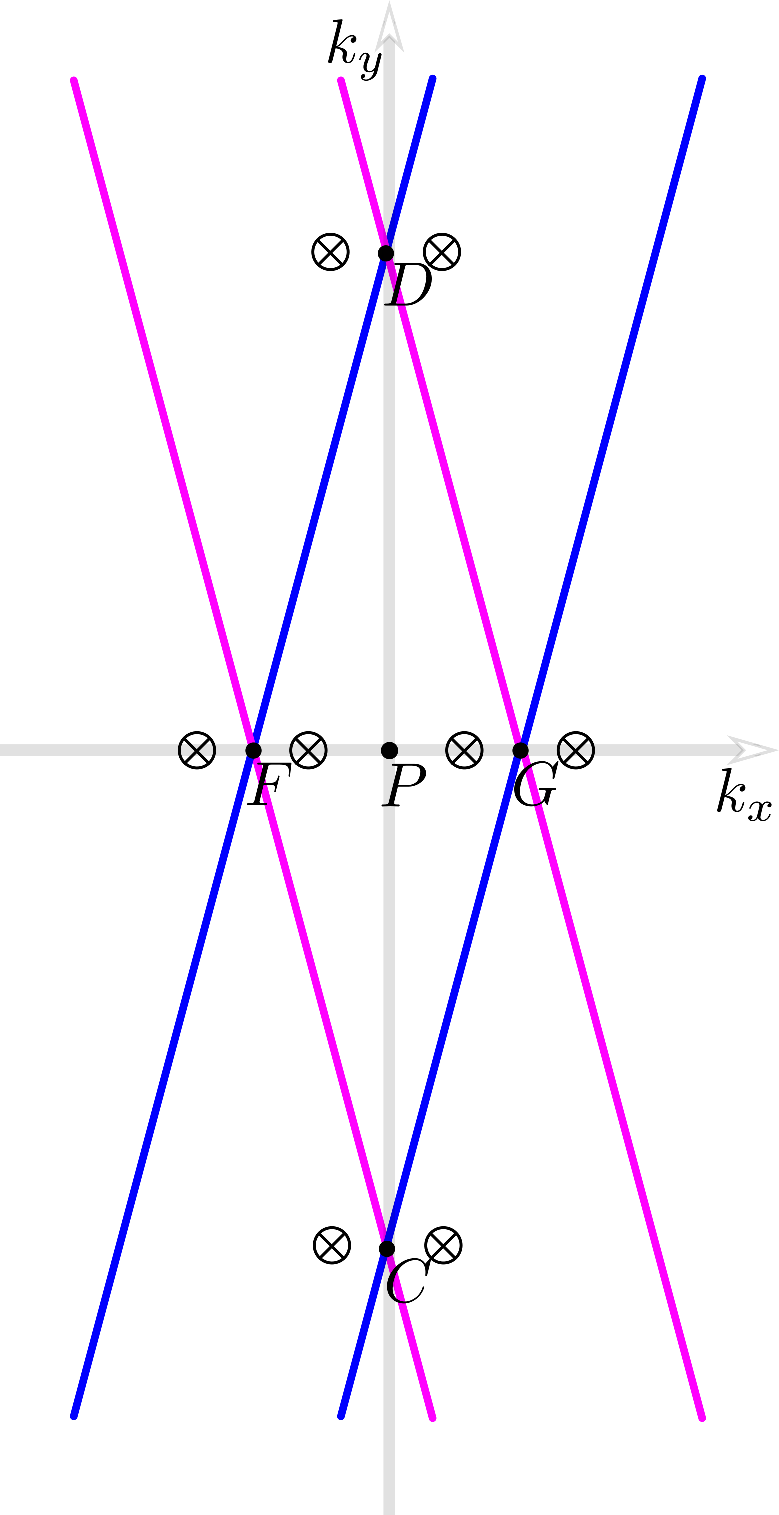
\includegraphics[scale=0.4]{contents/Ising_Top/figures/pdf_files/eight_nodes.pdf}
	\caption{{\bf Schematic Plot of Four Fermi Surface Intersection Points in a Twisted Bilayer Near Point-P}: When $\varphi=0$, each intersection point will give rise to two pairing nodes after $H_{\text{exch.}}$ is tuned up. When $\varphi\neq 0$, these nodes open up energy gaps: The four nodes near points $F$ and $G$ along the $\Gamma$-$M$ line have total Chern number zero. The four nodes near points $C$ and $D$ have total Chern number 4.}
	\label{fig: all eight nodes}
\end{figure}
The low energy effective theory near each point resembles Eq.(\ref{eqn:1layer}) with modified $v_F$ and $v_{\text{Ising}}$.

After $\Delta,\varphi$ are turned on but $\mu_B H_y=t_{s_y,\perp}=0$, the pairing gap minima near $C,D,F,G$ are found to be the same $\Delta_{C,D,F,G}=\Delta\sqrt{\cos^2\frac{\varphi}{2}+\cos^2\xi\sin^2\frac{\varphi}{2}}$, where $\xi$ is defined in Eq.(\ref{eqn:xi}).
Because the connection with the $\varphi=0$ limit, the superconducting phase so far must still be topologically trivial even though $\varphi\neq 0$ breaks the time-reversal symmetry.

When $\mu_B H_y,t_{s_y,\perp} \neq 0$ are tuned up, the behavior near the points $C,D$ versus $F,G$ are qualitatively different. The pairing gap minima near $F,G$ never go to zero as long as $\varphi\neq 0$. In particular, we find:
\begin{align}
	\Delta_{F,G}=\left\{\begin{array} {cc} \sqrt{(\Delta\cos\frac{\varphi}{2}-b)^2+\Delta^2\cos^2\xi\sin^2\frac{\varphi}{2}}, & b<\Delta\cos\frac{\varphi}{2}\\ \Delta\cos\xi|\sin\frac{\varphi}{2}|,&  b\geq \Delta\cos\frac{\varphi}{2}\end{array}\right.\label{eqn:gap_FG}
\end{align}
where
\begin{align}
	b\equiv
	\begin{cases}
		|\mu_B H_y\sin\xi -t_{s_y,\perp}|  & \mbox{ for point } F, \\
		|\mu_B H_y\sin\xi + t_{s_y,\perp}| & \mbox{ for point } G.
	\end{cases}
\end{align}

On the contrary, near points $C,D$ topological phase transition occurs with four Dirac nodes (two near each point) emerging when $H_y=H^{\text{topo.}}_{c}$, where the critical Zeeman field strength is
\begin{align}
	\mu_B H^{\mathrm{topo.}}_{c}\equiv\Delta\sqrt{\sec^2\xi\cos^2\frac{\varphi}{2}+\sin^2\frac{\varphi}{2}}.\label{eqn:Hc_topo}
\end{align}
When $H_y> H^{\mathrm{topo.}}_{c}$ the four Dirac nodes acquire topological mass gap, transferring a Chern number of 4:
\begin{align}
	\Delta^{\text{topo.}}_{C,D}=\sin\varphi\frac{\Delta^2\sin^2\xi}{\hbar v_{\text{Ising}}k_F\theta}\sqrt{\left(\frac{H_y}{H^{\text{topo.}}_{c}}\right)^2-1}\label{eqn:topo_gap}
\end{align}
The details of the calculations are presented in Appendix \ref{app:analytical}.

Note that different from $\Delta_{F,G}$, the topological gap $\Delta^{\text{topo.}}_{C,D}$ $\propto\Delta^2$. This is because $\Delta$-linear order gap remains zero in the present linear-order $\bm{k\cdot p}$ effective theory, and the second order perturbation plays the dominant role: the topological phase is always realized when $H_y>H^{\text{topo.}}_{c}$.

When a higher order $\bm{k\cdot p}$ expansion is considered, we do find that a non-topological $\Delta$-linear order gap near $C,D$ becomes nonzero (see Appendix \ref{app:analytical}). When this gap is large the topological superconductivity will be destroyed. Based on perturbative calculations, the topological phase requires the following criterion to be satisfied (See Appendix \ref{app:analytical} Eq.(\ref{eqn:v2_condition}) for details):
\begin{align}
	t_\perp^2      & < \frac{\Delta \hbar k_F v^2_{\text{Ising}}}{v_2}a(\xi,\varphi)\sqrt{\left(\frac{H_y}{H_c^{\text{topo.}}}\right)^2-1},\label{Phase boundary} \\
	a(\xi,\varphi) & \equiv \tan\xi\sin\xi\sqrt{\sec^2\xi\cos^2\frac{\varphi}{2}+\sin^2\frac{\varphi}{2}}.\nonumber
\end{align}
Here $v_2$ is a velocity parameter (defined in Eq.(\ref{eqn:v2_definition})) in the quadratic-order $\bm{k\cdot p}$ expansion, $\hbar v^{\text{NbSe}_2}_2=0.94$ and $\hbar v^{\text{TaS}_2}_2=3.1$ eV$\cdot$\AA based on our electronic structure calculations (See Appendix \ref{app:phase_diagram_details}). Namely, $t_\perp$ cannot be too large. This criterion serves as the phase boundary between the trivial and topological phases, and is plotted in FIG.\ref{fig:t-H phase digram} as the dashed black line.

The previous perturbative regime well captures the Chern-number-12 topological phase. Aiming at understanding the Chern-number-6 topological phase in the numerical phase diagrams, we have performed the analytical calculations in a different perturbative regime: $t_\perp\ll\Delta,\hbar v_{\text{Ising}}k_F\theta\ll\Delta$, and reproduced the Chern-number-6 topological phase (see Appendix \ref{app:analytical}).


\section{Discussion and conclusions}
Before concluding, we would like to remark on a few experiment-related issues.

\emph{Chiral edge modes:} When topological superconductivity is realized in the proposed heterostructure in Fig.\ref{fig: proposals}(a), the edge of the ferromagnetic buffer layer is the natural boundary between the topological superconductivity and trivial superconductivity. This is because outside the buffer layer region, due to the lack of Zeeman exchange field, gapped trivial superconductivity is realized in the TMD bilayer. Majorana chiral edge modes are then sharply located at this edge, leading to well-known quantized thermal Hall conductance $\frac{\kappa_{xy}}{T}=C\frac{\pi}{12}\frac{k_B^2}{\hbar}$, where $C$ is the Chern number. In addition, the edge modes can detected via scanning tunnelling microscopy as mid-gap states.

Mid-gap states located at the edge of a superconducting material has non-topological explanations, such as the Yu-Shiba-Rusinov bound states. However, in an appropriate regime, as shown in Fig.\ref{fig:theta-phi phase digram}, we note that a single device may realize trivial to topological phase transition while the Josephson phase $\varphi$ is tuned up. Such a $\varphi$-driven topological phase transition has unique experimental signatures since the majorana edge states are expected to exist only in the topological phase, which may be used to sharply identify the nature of the mid-gap states.

\vspace{1em}

\emph{The effect of in-plane external magnetic field:} When an in-plane magnetic field is applied to the proposed heterostructures, the Josephson phase $\varphi(x)=2\pi x/L$ becomes spatial dependent along the in-plane transverse direction, where $L=\frac{\Phi_0}{H_{\text{ext.}}d}$ and $d$ is the effective thickness of the junction. For instance, an external magnetic field $H_{ext.}\sim 0.5$T is needed to reorient the magnetic moment of CrBr$_3$ to an in-plane direction, corresponding to $L\sim 2\mu$m if $d\sim 20\text{\AA}$ is used. Due to the fact that the Chern number flips sign when $\varphi\rightarrow -\varphi$, the topological superconductivity is expect to form spatial stripes, or domains with width $L/2$, with alternating Chern numbers, e.g., $C=\pm12$ in which case 24 chiral majorana states are expected to form at each domain-wall. In Appendix \ref{app:domain_wall_modes} we estimate the spatial spread $l_\perp$  of the domain-wall majorana states along the transverse direction of the domain-wall. Only when $l_\perp$ is much smaller than the stripe width $L/2$ are the domain-wall states well-defined. We find that for a generic magnetic field direction $l_\perp$ is comparable with $L/2$ for $H_{ext.}\sim 0.5$T. However, when $H_{ext.}$ is parallel to one $\Gamma-M$ direction, 8 among the 24 domain-wall majorana states have an $l_\perp$ that can be $5\sim 10$ times smaller than $L/2$. These domain wall chiral states may be observable in probes such as STM or thermal transport.



\vspace{1em}
\emph{Charge-density-wave Order:} It is known that Ising superconductivity in 2H-$\mathrm{NbSe_2}$ or 2H-$\mathrm{TaS_2}$ coexists with the charge-density-wave (CDW) order \cite{ugeda2016characterization,xi2015strongly,nakata2018anisotropic}. For the Fermi pockets around $\Gamma$, the Fermi surface folding due to CDW occurs near the $\Gamma$-$K$ direction, which would not qualitatively affect the low energy physics near the $\Gamma$-$M$ direction, which we have been focusing on in this paper.

\vspace{1em}
\emph{Rashba Spin-orbit Coupling:} As emphasized before, the $z\rightarrow-z$ mirror symmetry forbids the Rashba spin-orbit coupling in the monolayer TMD. A Rashba spin-orbit coupling breaks an important invariance of Eq.(\ref{eqn:bilayer_bcs}) related to the combination of particle-hole and time-reversal transformation $\mathsf{PH}\circ\mathsf{TR}=\sigma_y\tau_x$. $\mathsf{PH}\circ\mathsf{TR}$ always sends $h_{\text{BCS}}^{\text{bilayer}}(\bm{k},H_y,\varphi)\mapsto -h_{\text{BCS}}^{\text{bilayer}}(\bm{k},-H_y,-\varphi)$. In the absence of the Rashba spin-orbit coupling one may flip the sign of $H_y$ and $\varphi$ by a complex conjugation since all other terms in the Hamiltonian are real: $-h_{\text{BCS}}^{\text{bilayer}}(\bm{k},-H_y,-\varphi)=-(h_{\text{BCS}}^{\text{bilayer}})^*(\bm{k},H_y,\varphi)$. Namely there is an invariance protecting the Bogoliubov quasiparticle spectrum being $\pm E$ symmetric at any $\bm k$. Such an invariance is lost in the presence of a Rashba spin-orbit coupling, leading to Bogoliubov Fermi pockets \cite{shaffer2020crystalline}.

In the proposed heterostructures, despite the lack of the $z\rightarrow-z$ mirror symmetry, the intrinsic Rashba coupling induced by the vdW interlayer interactions can be safely neglected since it is extremely weak (see in Appendix \ref{app:phase_diagram_details}). Although an extrinsic, substrate-induced Rashba coupling is possible, in this paper we do not consider this effect, since nevertheless this coupling could be tuned to zero via gating.

\vspace{1em}
\emph{Interlayer Tunneling Strength:} It is clear from the phase diagrams in FIG. \ref{fig:t-H phase digram} and criterion Eq.(\ref{Phase boundary}) that the interlayer tunneling $t_\perp$ cannot be too large in order to realize the topological superconductivity ($<10$meV). On the other hand, based on our DFT calculation (see Appendix \ref{app:phase_diagram_details}), due to the $d_{z^2}$ nature of Fermi pockets around $\Gamma$-point, a fairly large interlayer tunneling of the bilayer systems of $\mathrm{NbSe_2}$ or $\mathrm{TaS_2}$ \emph{without} a buffer layer is found near the point-$P$ ($>50$meV) \footnote{In literature \protect\url{https://www.nature.com/articles/s41467-018-03888-4}, a smaller value of tunneling about 15meV for bilayer $\mathrm{NbSe_2}$ is reported. We ascribe such discrepancy to the choice of van der Waals pseudopotentials.}. This actually motivates us to consider the insulating buffer layer in the proposed heterostructures. In Appendix \ref{app:phase_diagram_details}, as an estimate, we performed DFT calculations on a $\mathrm{TaS_2}/\mathrm{WS_2}/\mathrm{TaS_2}$ heterostructure, and $t_\perp\sim 5$meV is found -- well within the regime where topological superconductivity is realized.

\vspace{1em}
In summary, we theoretically propose twisted bilayer vdW Ising superconductors as a new flexible and tunable platform to realize chiral topological superconductivity with Chern numbers. In the simplest setup, an insulating buffer layer with an in-plane ferromagnetic moment is introduced between the TMD Ising superconductors such as $\mathrm{NbSe_2}$ or $\mathrm{TaS_2}$, providing Zeeman exchange field in the TMD layers via the magnetic proximity effect. We show that the out-of-plane supercurrent induces topological superconductivity over a large parameter regime, and the characteristic majorana chiral edge modes are localized on the edge of the ferromagnetic buffer layer. We hope that the present study may motivate further experimental and theoretical investigations on such vdW heterostructures.


\begin{subappendices}
	\section{Domain-wall chiral modes}\label{app:domain_wall_modes}
	Assuming inter-node scattering being weak, here we may use the Dirac equation for a single node to estimate the spatial size of the chiral domain-wall modes. Denoting the magnetic field direction as $\hat B$, we have the spatial-dependent Josephson phase $\varphi(\bm r)=\frac{2\pi}{L}\hat B\times\hat z  \cdot \bm r\equiv \frac{2\pi}{L}\hat n\cdot \bm r$, where we defined unit vector $\hat n\equiv \hat B\times \hat z$. Based on Eq.(\ref{eqn:topo_gap}), the spatial-dependent Dirac equation becomes:
	\begin{align}
		H=v_x p_x\Sigma_x+v_y p_y\Sigma_z+m_0\sin\varphi(\bm r)\Sigma_y,
	\end{align}
	where
	\begin{align}
		m_0\equiv\frac{\Delta^2\sin^2\xi}{\hbar v_{\text{Ising}}k_F\theta}\sqrt{\Big(\frac{H_y}{H^{\text{topo.}}_{c}}\Big)^2-1}.
	\end{align}
	$v_x=v_F\cos\theta^+$ and $v_y=v_{\text{Ising}}\sin\theta^+$ according to Eq.(\ref{heff for P+ and P-}), and $v_x\gg v_y$ since $\theta^+$ is an angle parameter of order unity.
	The mass-sign-changing domain walls are located at $\hat n\cdot \bm r=\frac{k L}{2}$, and $k\in\mathbb{Z}$. Near each domain wall, we may linearize the mass as $m_0\sin\varphi(\bm r)\sim (-1)^k m_0\tilde \varphi(\delta \bm r)$, where $\tilde\varphi(\delta \bm r)=\varphi(\bm r)-k\pi=\frac{2\pi\hat n\cdot \delta\bm r}{L}$, and $\delta \bm r$ is the position measured from the domain wall.

	It is now convenient to rotate into the coordinate system with axes $(x_\parallel,x_\perp)$ along and perpendicular to the domain-wall. The corresponding momentum are denoted as $(p_\parallel,p_\perp)$. Writing the cosine $c$ and sine $s$ of the rotation angle between the two coordinate systems, then $p_x\equiv c p_\parallel- s p_\perp$ and $p_y\equiv s p_\parallel+c p_\perp$, and we have
	\begin{align}
		H & =v_x (c p_\parallel- s p_\perp)\Sigma_x+v_y (s p_\parallel+c p_\perp)\Sigma_z\nonumber \\
		  & \qquad+(-1)^k m_0\frac{2\pi x_\perp}{L}\Sigma_y,
	\end{align}
	$H^2$ has a simple form:
	\begin{align}
		H^2 & =v_x^2(c p_\parallel- s p_\perp)^2+v_y^2(s p_\parallel+c p_\perp)^2+m_0^2\left(\frac{2\pi x_\perp}{L}\right)^2\notag \\
		    & -(-1)^k \hbar m_0\frac{2\pi}{L}(sv_x\Sigma_z+c v_y\Sigma_x)
	\end{align}
	Since $p_\parallel$ is a good quantum number we are left with a one-dimensional harmonic oscillator involving $p_\perp,x_\perp$:
	\begin{align}
		H^2 & =\big((cv_x)^2+(sv_y)^2\big)p_\parallel^2+\big((sv_x)^2+(cv_y)^2\big)(p_\perp - p_0(p_\parallel) )^2\notag \\
		+   & m_0^2\left(\frac{2\pi x_\perp}{L}\right)^2-(-1)^k \hbar m_0\frac{2\pi}{L}(sv_x\Sigma_z+c v_y\Sigma_x),
	\end{align}
	where $p_0$ is a linear function of $p_\parallel$. The corresponding mass and frequency for this harmonic oscillator are:
	\begin{align}
		M      & =\frac{1}{2}[(sv_x)^2+(cv_y)^2]^{-1}\notag \\
		\omega & =\sqrt{2M^{-1}}\frac{m_02\pi}{L}.
	\end{align}
	The energy levels are:
	\begin{align}
		E_n=2\hbar\sqrt{(sv_x)^2+(cv_y)^2}\frac{m_02\pi}{L}(n+\frac{1}{2}).
	\end{align}
	The zero energy state of $H$ and $H^2$ for $p_\parallel=0$, corresponding to the chiral majorana modes, is the $n=0$ ground state of the harmonic ocsillator. The last term in $H^2$ chooses a specific eigenstate of $(sv_x\Sigma_z+c v_y\Sigma_x)$, so that the zero-point energy in the harmonic oscillator is exactly canceled. Since we are working with complex fermion, this zero energy state corresponds to two chiral majorana modes.

	The spatial spread $l$ of the chiral model along the $x_\perp$ direction can be readily read out from the harmonic oscillator ground state $\psi(x_\perp)\propto e^{-x_\perp^2/(2l_\perp^2)}$:
	\begin{align}
		l_\perp & =\sqrt{\frac{\hbar}{M\omega}}=\sqrt{\frac{\hbar [(sv_x)^2+(cv_y)^2]^{1/2} L}{2\pi m_0}}
	\end{align}

	$l_\perp$ is proportional to the square root of the velocity $[(sv_x)^2+(cv_y)^2]^{1/2}$. Note that $v_x\gg v_y$, for a generic magnetic field direction, $l_\perp\sim \sqrt{\frac{\hbar v_x L}{2\pi m_0}}$. Assuming $\hbar v_x\sim 1\mathrm{eV}\cdot\text{\AA}$, $m_0\sim 0.1\mathrm{meV}$, and $L\sim 2\mathrm{\mu m}$, one finds $l_\perp\sim 0.4\cdot L/2$.

	To minimize $l_\perp$, one may choose the magnetic field direction (i.e., the domain-wall direction) being along $x$ (i.e., one $\Gamma$-$M$ direction), leading to $l_\perp=\sqrt{\frac{\hbar v_y L}{2\pi m_0}}$ for 4 nodes near this $\Gamma$-$M$ direction among the total of 12 nodes. In this case, among the 24 majorana domain wall states, 8 of them have $l_\perp\sim 0.2\cdot L/2$ (for TaS$_2$) and $l_\perp\sim 0.1\cdot L/2$ (for NbSe$_2$) using the parameters above.

	\section{A mean-field treatment for the ferromagnetic buffer layer}\label{app:magnetic_buffer_layer_perturbation}
	We will show in this section that, for the proposed setup in Fig.\ref{fig: proposals}(a) with a ferromagnetic buffer layer, the direct couplings between the top/bottom layer and the middle layer will induce an in-plane exchange Zeeman-field $H_{\text{exch.}}$, and a spin-dependent tunneling $t_{s,\perp}$. In a simple perturbative mean-field treatment, $\mu_B H_{\text{exch.}}=t_{s,\perp}$.


	Without loss of generality, we can work in the basis where the buffer layer Hamiltonian is diagonalized $\bm{h}^\text{m}=\mathop{\mathrm{diag}}\{h^{\text{m}}_\uparrow, h^\text{m}_\downarrow\}$, where $\uparrow$ and $\downarrow$ indicate the spin components parallel and antiparallel to \emph{the in-plane ferromagnetic moment direction}. For simplicity we assume $h^{\text{m}}_\uparrow$, $h^{\text{m}}_\downarrow$ each contains a single band, which can be easily generalized to multi-band cases.


	In the absence of the middle layer, we consider the spinful TMD bilayer Hamiltonian $\bm{h}^\text{bilayer}=\mathop{\mathrm{diag}}\{\bm{h}^\text{t}(\bm{k}), \bm{h}^\text{b}(\bm{k})\}$. The full Hamiltonian for the trilayer system is then:
	\begin{equation}\label{trilayer Hamiltonian}
		H^{\text{trilayer}}(\bm{k})=\left(\begin{array}{c|c}
				\begin{matrix}
					\bm{h}^\text{t}(\bm{k}) &                         \\
					                        & \bm{h}^\text{b}(\bm{k})
				\end{matrix} & \text{\Large $\bm{V}$}                                                  \\
				\hline
				\text{\Large $\bm{V}^T$}                             & \begin{matrix}
					                                                       h^\text{m}_\uparrow &                       \\
					                                                                           & h^\text{m}_\downarrow
				                                                       \end{matrix}
			\end{array}\right),
	\end{equation}
	where $\bm{V}=(\bm{V}_1,\bm{V}_2)$, $\bm{V}_1=(t^\text{t}_\uparrow,0,t^\text{b}_\uparrow,0)^T$, and $\bm{V}_2=(0,t^\text{t}_\downarrow,0,t^\text{b}_\downarrow)^T$.\par
	Due to the $z\rightarrow -z$ mirror symmetry for the TMD bilayer at the zero twisting angle, one may assume these direct hoppings to be layer-independent $t^{\text{t,b}}_{\uparrow,\downarrow}=t_{\uparrow,\downarrow}$ at small twisting angles. Since the middle buffer layer is an insulator, 	$h^\text{m}_\uparrow,	h^\text{m}_\uparrow$ are high energy states. Standard perturbation theory gives
	\begin{align}
		 & H^{\text{bilayer}}_\text{induced}(\bm{k})\simeq \bm{h}^{\text{bilayer}}-\sum_{i=1,2} \bm{V}_i(\bm{h}^\text{m})^{-1}\bm{V}_i^T\nonumber                                    \\
		 & =\bm{h}^{\text{bilayer}}-\dfrac{t_\uparrow^2}{h^\text{m}_\uparrow}\left(\begin{array}{cccc}
				                                                                           1 & 0 & 1 & 0 \\
				                                                                           0 & 0 & 0 & 0 \\
				                                                                           1 & 0 & 1 & 0 \\
				                                                                           0 & 0 & 0 & 0
			                                                                           \end{array}\right)-\dfrac{t_\downarrow^2}{h^\text{m}_\downarrow}\left(\begin{array}{cccc}
				                                                                                                                                                 0 & 0 & 0 & 0 \\
				                                                                                                                                                 0 & 1 & 0 & 1 \\
				                                                                                                                                                 0 & 0 & 0 & 0 \\
				                                                                                                                                                 0 & 1 & 0 & 1
			                                                                                                                                                 \end{array}\right)\nonumber \\
		 & =\bm{h}^{\text{bilayer}}-\delta\mu\sigma_0\nu_0+t_\perp\sigma_0\nu_x+\mu_B H_{\text{exch.},z}\sigma_z\nu_0+t_{s,\perp}\sigma_z\nu_x,\label{proximity-induced Heff}
	\end{align}
	where we separate out the second-order perturbation of bilayer Hamiltonian into four parts: the chemical potential shift $\delta\mu$, the spin-independent tunneling $t_\perp$, the (proximity-induced) Zeeman field $H_{\text{exch.}}$, and the spin-dependent tunneling $t_{s,\perp}$, where.
	\begin{align}
		-\delta\mu            & = t_\perp=-\dfrac{1}{2}\left(\dfrac{t^2_\uparrow}{h^\text{m}_\uparrow}+\dfrac{t^2_\downarrow}{h^\text{m}_\downarrow}\right),\label{proximity-induced constraint: mu and t_perp}          \\
		\mu_BH_{\text{exch.}} & =t_{s,\perp}=-\dfrac{1}{2}\left(\dfrac{t^2_\uparrow}{h^\text{m}_\uparrow}-\dfrac{t^2_\downarrow}{h^\text{m}_\downarrow}\right).\label{proximity-induced constraint: h_exch and t_s,perp}
	\end{align}

	\section{Details of the phase diagram calculations and discussions on the  stacking-dependence}\label{app:phase_diagram_details}
	All phase diagrams of the proposed heterostructures involving either 2H-NbSe$_2$ or 2H-TaS$_2$ are obtained by listing the gap size for all eight nodes (topological and trivial) and picking out the \emph{minima} of them. To capture the physics among entire phase-diagrams (particularly the large-$H_\text{exch.}$ regions), we follow Ref.\cite{xi2016ising} to introduce the pair breaking equation throughout our numerical calculation
	\begin{equation*}
		\ln(T_c/T_{c0})+\psi\left(\dfrac{1}{2}+\dfrac{\mu_B H^2/H_{\text{so}}}{2\pi k_B T_c}\right)-\psi(1/2)\equiv0,
	\end{equation*}
	where $\psi$ is the digamma function, $T_{c0}$ is the zero-field critical temperature ($3.0$K for $\mathrm{NbSe_2}$ \cite{xi2016ising} and $3.4$K for $\mathrm{TaS_2}$ \cite{yang2018enhanced}), and $H_{\text{so}}$ can be taken as a fitting parameter to match the asymptotic Ginzberg-Landau behavior $H\sim H_0\sqrt{1-T/T_{c0}}$ for $T_c\sim T_{c0}$, where $H_0\sim\sqrt{H_{\text{so}}H_p}$ and the Pauli limit  $H_p=\frac{\Delta_0}{\sqrt{2}\mu_B}=(1.86~\mathrm{T/K})\cdot T_{c0}$ assuming the $g$-factor equals to 2 and the BCS formula $\Delta_0=1.76k_B T_{c0}$ still to hold \footnote{For few-layer $\mathrm{TaS_2}$, the relation is also reported to be $\Delta_0=2.2k_B T_{c0}$ in \protect\url{https://www.nature.com/articles/s41563-018-0061-1}. Since such coefficient is material- and stacking-dependent, we will still take the value of BCS approximation $\Delta_0=1.76k_B T_{c0}$ as a demonstration.}. The best fitting of experimental data gives $H_0=43.6\mathrm{T}$ for $\mathrm{NbSe_2}$ and $H_0=65.6\mathrm{T}$ for $\mathrm{TaS_2}$ \cite{de2018tuning}, so we take $H_{\text{so}}^{\mathrm{NbSe_2}}=340\mathrm{T}$ and $H_{\text{so}}^{\mathrm{TaS_2}}=680\mathrm{T}$ throughout our numerical calculations.\par
	All parameters we input in our numerical calculations of phase diagrams (up to fourth-order of $\bm{k\cdot p}$ expansion) are extracted from the monolayer tight-binding models obtained from LDA calculation by QUANTUM ESPRESSO \cite{giannozzi2009quantum,giannozzi2017advanced} and Wannier90 routine \cite{pizzi2020wannier90}. Our strategies is to first build a AA-stacking $\beta$-bilayer slab system for both materials, then relax the structure with non-local van de Waals correlation functionals to get the proper layer distance and (spin-independent) tunneling strengths. For convergence reasons, we choose to use the functional vdW-DF-C6 \cite{tkatchenko2009accurate,berland2019van} for $\mathrm{TaS_2}$ while vdW-DF2-C09 \cite{lee2010higher,cooper2010van} for $\mathrm{NbSe_2}$. The resulting relaxed layer separation is $d_\perp^{\mathrm{TaS_2}}=6.57\text{\AA}$ and $d_\perp^{\mathrm{NbSe_2}}=6.80\text{\AA}$. Since tunneling processes only occur around the interesction points $P$, with their strengths to be half of the energy splitting around the Fermi energy $\varepsilon_F$, we can directly read them out from the the non self-consistent output at $\bm{k}=(k_F,0)$, reading $t_\perp^{\mathrm{TaS_2}}=56.9\mathrm{meV}$ and $t_\perp^{\mathrm{NbSe_2}}=116.2\mathrm{meV}$.\par
	Next, we take the relaxed structure as an input to build a monolayer slab system and perform a LDA calculation to obtain a monolayer electronic structure. Note that this monolayer relaxed structure weakly breaks the $z\rightarrow -z$ symmetry, but preserves the mirror planes parallel with the $z$-axis. The LDA result is used to fit the $\bm{k\cdot p}$ model up to quartic order. More precisely, we fit the model consistent with the $y\rightarrow -y$ mirror symmetry:
	\begin{align}\label{monolayer quartic kdotp expansion}
		H^{\text{mono}}_{\text{quartic}}(\bm{k}) & =\bigg[\varepsilon_F +v_F k_x + a k_y^2 + p_5 k_x^2 + p_6 k_x k_y^2\nonumber                 \\
		                                         & \quad + p_7 k_y^4 + p_8 k_x^3 + p_9 k_x^4 + p_{10} k_x^2 k_y^2\bigg]\sigma_0\nonumber        \\
		                                         & \quad + p_{11}\sigma_y +\bigg[ v_{\text{Ising}} k_y + p_{13} k_x k_y + p_{14} k_y^3\nonumber \\
		                                         & \quad + p_{15} k_x^2 k_y + p_{16} k_x^3 k_y + p_{17} k_x k_y^3\bigg]\sigma_z.
	\end{align}
	The results for both $\mathrm{TaS_2}$ and $\mathrm{NbSe2}$ are listed as following: (in the eV-\AA~unit system and we set $\hbar=1$, as a complement of the TABLE.\ref{table:parameters} given in the main text)

	\begin{center}
		\begin{tabular}{c|ccccccccccccccccc}
			\hline\hline
			\diagbox{Materials}{Coef. $p_i$} & $k_F$ & $v_F$ & $a$   & $p_5$ & $p_6$ & $p_7$ & $p_8$ & $p_9$ \\
			\hline
			$\mathrm{TaS_2}$                 & 0.54  & -2.89 & 0.25  & 2.34  & 17.82 & -8.72 & 11.53 & -8.67 \\
			\hline
			$\mathrm{NbSe_2}$                & 0.48  & -2.22 & -0.76 & 1.36  & 15.10 & -2.98 & 9.85  & -0.76 \\
			\hline\hline
		\end{tabular}
		\vspace*{5mm}
		\begin{tabular}{c|ccccccccc}
			\hline\hline
			\diagbox{Materials}{Coef. $p_i$} & $p_{10}$ & $p_{11}$ & $v_{\text{Ising}}$ & $p_{13}$ & $p_{14}$ & $p_{15}$ & $p_{16}$ & $p_{17}$ \\
			\hline
			$\mathrm{TaS_2}$                 & 17.20    & 0.00     & 0.36               & 1.41     & -1.06    & -0.72    & -2.11    & -8.45    \\
			\hline
			$\mathrm{NbSe_2}$                & 26.15    & 0.00     & 0.12               & 0.86     & -0.20    & 0.25     & -3.56    & -4.14    \\
			\hline\hline
		\end{tabular}
	\end{center}

	The intrinsic Rashba SOC, ignored in Eq.\eqref{eqn:1layer}, appears as the vanishingly small $p_{11}$ in the above fitting. Due to the loss of the $z\rightarrow -z$ mirror symmetry in the vdW relaxed structure, in principle this coupling may be nonzero. However, we find that the raw energy splittings (corresponding to $2p_{11}$) at the point-$P$ is less than $10^{-10}\text{meV}$ for both $\mathrm{NbSe_2}$ and $\mathrm{TaS_2}$, and conclude that weak vdW interactions cannot lead to any sizable intrinsic Rashba SOC.

	The values of aforementioned spin-independent tunnelings $t_\perp$ for bilayer $\mathrm{NbSe_2}$ and $\mathrm{TaS_2}$ are far beyond the topological superconducting regime that we find in the numerical phase diagrams. That actually motivates us to propose the buffer layer heterostructures in FIG.~\ref{fig: proposals}. To have an estimation on the magnitude of the spin-independent tunneling $t_\perp$ \emph{after} the insertion of an insulating buffer layer, we build a trilayer slab system $\mathrm{TaS_2}/\mathrm{WS_2}/\mathrm{TaS_2}$ of ABA and AAA stackings. Since $\mathrm{2H}$-$\mathrm{TaS_2}$ and $\mathrm{2H}$-$\mathrm{WS_2}$ have similar lattice constants, we use the lattice constants of $\mathrm{2H}$-$\mathrm{TaS_2}$ for the trilayer system without enlarging the supercell \footnote{We use the crystalline data from Spinger Materials, see \protect\url{https://materials.springer.com/isp/crystallographic/docs/sd_0457067} and \protect\url{https://materials.springer.com/isp/crystallographic/docs/sd_0551013}.} ($a=0.331$nm and $c=0.121$nm for $\mathrm{2H}$-$\mathrm{TaS_2}$, and $a=0.315$nm and $c=0.121$nm for $\mathrm{2H}$-$\mathrm{WS_2}$). We then again relax the positions for all atoms of the trilayer system with the non-local van der Waals functional vdW-DF-C6 \cite{tkatchenko2009accurate,berland2019van} along the out-of-plane direction. We find, after an inserting of a non-magnetic buffer layer $\mathrm{WS_2}$, the separation between top and bottom $\mathrm{TaS_2}$ layers for both stackings almost doubles to $d_\perp^{\mathrm{TaS_2},\text{ABA}}=12.00\text{\AA}$ and  $d_\perp^{\mathrm{TaS_2},\text{AAA}}=13.18\text{\AA}$, and the corresponding strengths of the spin-independent tunneling reduce to $t_\perp^{\mathrm{TaS_2},\text{ABA}}=5.0\mathrm{meV}$ and $t_\perp^{\mathrm{TaS_2},\text{AAA}}=4.5\mathrm{meV}$.


	\section{Details of analytical perturbative calculations}\label{app:analytical}
	We will work with the atomic units by default throughout the derivation here. For example, $\hbar=\mu_B=1$.
	\hfill\\
	\subsection{Perturbative theory for $\sqrt{(v_{\text{Ising}}k_F\theta)^2+4t_\perp^2}\gg \Delta $: $C=12$ Topological Phases}
	In this section, we will give a perturbative analysis on the twisted bilayer Hamiltonian given in the main text. We will focus on the regime when $\sqrt{(v_{\text{Ising}}k_F\theta)^2+4t_\perp^2}\gg \Delta $ and give an explanation on the origin of $C=\pm12$ topological phases. Mass gaps for all nodes and the phase boundary will also be also derived.
	\subsubsection{Construction of Hamiltonian}
	Let us start with constructing the effective Hamiltonian. We will consider a small twisting angle $\theta$, and keep the $\bm{k\cdot p}$ expansion up to $\mathcal{O}(\theta^2)$ (the reason will be given in the next subsection). As is discussed in the main text, in-plane mirror symmetry prohibit the existence of Rashba SOC, so the monolayer effective Hamiltonian around the intersection point $P$ of the Fermi surface and the $\Gamma$-$M$ line simply reads
	\begin{equation}\label{monolayer Hamiltonian}
		h^{\text{mono}}(\bm{k})=(v_F k_x + a k_y^2)+v_{\text{Ising}} k_y \sigma_z,
	\end{equation}
	where $a$ is the coefficient of $\bm{k\cdot p}$ expansion. We keep a quadratic term $ak_y^2$ here because it turns out that this term contributes to the leading order deviation from the linear $\bm{k\cdot p}$ expansion. Equation \eqref{monolayer Hamiltonian} can be easily extend to higher orders and we did use the fitting fourth-order $\bm{k\cdot p}$ in our numerical calculations, see section V.\par
	Without loss of generality, we can consider a bilayer system with the top layer rotated by $\theta/2$, and the bottom layer rotated by $-\theta/2$. This is achieved by simple replacement $k_x\mapsto(k_x+k_F)\cos\frac{\theta}{2}\pm k_y\sin\frac{\theta}{2}-k_F$ and $k_y\mapsto\mp(k_x+k_F)\sin\frac{\theta}{2}+k_y\cos\frac{\theta}{2}$ and expansion still up to $\theta^2$. The resulting bilayer Hamiltonian \emph{without} tunneling is then

	\begin{align}\label{bilayer Hamiltonian without Tunneling}
		h^{\text{bilayer w/o tunneling}}(\bm{k}) & =\left(v_F k_x+ak_y^2+\dfrac{ak_F^2}{4}\theta^2-\dfrac{v_F k_F}{8}\theta^2\right)+\left(-ak_F k_y \theta+\dfrac{\theta}{2}v_F k_y\right)\nu_z\nonumber \\
		                                         & \quad+v_{\text{Ising}} k_y\sigma_z-v_{\text{Ising}} k_F\dfrac{\theta}{2}\sigma_z\nu_z \nonumber                                                        \\
		                                         & =\left(v_F k_x+ak_y^2-\dfrac{v_2 k_F}{8}\theta^2\right)+\dfrac{\theta}{2}v_2k_y\nu_z+v_{\text{Ising}} k_y\sigma_z\nonumber                             \\
		                                         & \quad-\dfrac{\theta}{2}v_{\text{Ising}} k_F\sigma_z\nu_z,
	\end{align}

	where $\nu_i$ are Pauli matrices within the layer space and we defined
	\begin{equation}
		v_2\equiv v_F-2ak_F.\label{eqn:v2_definition}
	\end{equation}
	In Eq.(\ref{bilayer Hamiltonian without Tunneling}), the crucial role played by $v_2$ is due to the second term, which gives the leading order correction to the wavefunctions comparing with the linear $\bm{k\cdot p}$ expansion.
	\indent Next, let us try to add interlayer tunnelings to \eqref{bilayer Hamiltonian without Tunneling}. Based on \emph{two-center approximation} \cite{bistritzer2011moire}, it can be shown that (see in Appendix \ref{app:magnetic_buffer_layer_perturbation}) the interlayer tunneling have a weak spatial-dependence and will be considered as a constant here $t=t_\perp$ (we will consider the spin-dependent tunnelings $t_{s,\perp}$ later). We thus have
	\begin{align}\label{bilayer Hamiltonian}
		h^{\text{bilayer}} & =\left(v_F k_x+ak_y^2-\dfrac{v_2k_F^2}{8}\theta^2\right)\nonumber                                                           \\
		                   & \quad+\dfrac{\theta}{2}v_2 k_y\nu_z+v_{\text{Ising}} k_y\sigma_z-\dfrac{\theta}{2}v_{\text{Ising}} k_F\sigma_z\nu_z+t\nu_x.
	\end{align}
	Hamiltonian \eqref{bilayer Hamiltonian} reduce to simple two-band model \cite{bernevig2013topological} (so can be readily diagonalized) for $\sigma_z=\pm1$. Keeping up to $\mathcal{O}(\theta^2)$, we have, for $\sigma_z=+1$,
	\begin{align*}
		\varepsilon_\pm^\uparrow & =\left(v_F k_x +a k_y^2-\dfrac{\theta^2}{8}v_2 k_F\right)+v_{\text{Ising}}k_y\pm\dfrac{\Gamma}{2}\left[1-\dfrac{v_2\cdot\cos^2\xi}{v_{\text{Ising}} k_F}k_y\right]
	\end{align*}
	and for $\sigma_z=-1$,
	\begin{equation*}
		\varepsilon^\downarrow_\pm=\left(v_F k_x +a k_y^2-\dfrac{\theta^2}{8}v_2 k_F\right)-v_{\text{Ising}}k_y\pm\dfrac{\Gamma}{2}\left[1+\dfrac{v_2\cdot\cos^2\xi}{v_{\text{Ising}} k_F}k_y\right],
	\end{equation*}
	where
	\begin{equation*}
		\xi\equiv \arctan\dfrac{2t}{v_{\text{Ising}} k_F \theta},\quad\text{and}\quad\Gamma\equiv\sqrt{(v_{\text{Ising}}k_F\theta)^2+4t^2}.
	\end{equation*}

	There are some crossing points between the spin-up and spin-down Fermi surfaces. Solving $\varepsilon_\pm^\uparrow=\varepsilon_\pm^\downarrow=0$, we find two such points $F$ and $G$ along the $k_x$ direction ($\Gamma$-$M$ line)
	\begin{equation}\label{F,G coordinates withouth Delta and phi}
		F=\left(-\dfrac{\Gamma}{2v_F}+\dfrac{v_2k_F\theta^2}{8v_F}, 0\right),\quad G=\left(+\dfrac{\Gamma}{2v_F}+\dfrac{v_2k_F\theta^2}{8v_F}, 0\right).
	\end{equation}
	At $F$, the two low energy bands come from $\varepsilon_-^{\uparrow,\downarrow}$, while at $G$, the two low energy bands are formed by $\varepsilon_+^{\uparrow,\downarrow}$. Interestingly, there are another two such points $C$ and $D$ emergent along the $k_y$-direction that have different low-energy bands information. We also have
	\begin{align}
		C & =\left(-\dfrac{k_F\theta^2}{8}-\dfrac{a t^2}{v_Fv_{\text{Ising}}^2}, -\dfrac{\Gamma}{2v_{\text{Ising}}}\right),\label{C coordinates withouth Delta and phi} \\
		D & =\left(-\dfrac{k_F\theta^2}{8}-\dfrac{a t^2}{v_Fv_{\text{Ising}}^2}, +\dfrac{\Gamma}{2v_{\text{Ising}}}\right).\label{D coordinates withouth Delta and phi}
	\end{align}
	At $C$, the two low-energy bands are formed by $\varepsilon_-^\uparrow,\varepsilon_+^\downarrow$, while at $D$, the two low-energy bands are formed by $\varepsilon_+^\uparrow,\varepsilon_-^\downarrow$. They are all illustrated in the main text. In the following derivation, we will denote the $\bm{k}$-space coordinates of the intersection points $F$ as $\bm{F}_+$, $G$ as $\bm{F}_-$, $C$ as $\bm{C}_-$, and $D$ as $\bm{C}_+$.\par
	The low-energy effective Hamiltonian of each node is then the projection of \eqref{bilayer Hamiltonian} onto these bands. First of all, we need to read out the eigenstates in $\nu$-space. Introducing the elevation angle
	\begin{align*}
		\xi_\pm & =\arctan\dfrac{t}{\frac\theta 2(v_2k_y-v_{\text{Ising}} k_F)}                                                           \\
		        & \simeq\arctan\left[\left(1\pm\dfrac{v_2k_y}{v_{\text{Ising}} k_F}\right)\dfrac{2t}{v_{\text{Ising}} k_F \theta}\right],
	\end{align*}
	we obtain:
	\begin{align*}
		\sigma_z=+1: & \quad|\nu_1\rangle=\sin\frac{\xi_+}{2}|\nu_\uparrow\rangle+\cos\frac{\xi_+}{2}|\nu_\downarrow\rangle,  \\
		             & \quad|\nu_2\rangle=\cos\frac{\xi_+}{2}|\nu_\uparrow\rangle-\sin\frac{\xi_+}{2}|\nu_\downarrow\rangle,  \\
		\sigma_z=-1: & \quad|\nu_3\rangle=\cos\frac{\xi_-}{2}|\nu_\uparrow\rangle+\sin\frac{\xi_-}{2}|\nu_\downarrow\rangle,  \\
		             & \quad|\nu_4\rangle=-\sin\frac{\xi_-}{2}|\nu_\uparrow\rangle+\cos\frac{\xi_-}{2}|\nu_\downarrow\rangle.
	\end{align*}
	We can then lift \eqref{bilayer Hamiltonian} into Nambu representation

	\begin{equation}\label{bilayer Hamiltonian in Nambu}
		H^{\text{bilayer}}=\left(v_F k_x+ak_y^2-\dfrac{v_2 k_F}{8}\theta^2\right)\tau_z+\dfrac{\theta}{2}v_2k_y\nu_z\tau_z+v_{\text{Ising}} k_y\sigma_z-\dfrac{\theta}{2}v_{\text{Ising}} k_F\sigma_z\nu_z+t\nu_x\tau_z,
	\end{equation}
	and perform the projection. Here $\nu_i$ are Pauli matrices for the Nambu space.\par
	Choosing the basis as following
	\begin{align*}
		\text{At }G: & \quad \{|\tau_\uparrow,\sigma_\uparrow,\nu_2\rangle,|\tau_\uparrow,\sigma_\downarrow,\nu_4\rangle,|\tau_\downarrow,\sigma_\uparrow,\nu_4\rangle,|\tau_\downarrow,\sigma_\downarrow,\nu_2\rangle, |\tau_\uparrow,\sigma_\uparrow,\nu_1\rangle,|\tau_\uparrow,\sigma_\downarrow,\nu_3\rangle, \\
		             & \quad|\tau_\downarrow,\sigma_\uparrow,\nu_3\rangle,|\tau_\downarrow,\sigma_\downarrow,\nu_1\rangle\},                                                                                                                                                                                       \\
		\text{At }F: & \quad \{|\tau_\uparrow,\sigma_\uparrow,\nu_1\rangle,|\tau_\uparrow,\sigma_\downarrow,\nu_3\rangle,|\tau_\downarrow,\sigma_\uparrow,\nu_3\rangle,|\tau_\downarrow,\sigma_\downarrow,\nu_1\rangle,|\tau_\uparrow,\sigma_\uparrow,\nu_2\rangle,|\tau_\uparrow,\sigma_\downarrow,\nu_4\rangle,  \\
		             & \quad|\tau_\downarrow,\sigma_\uparrow,\nu_4\rangle,|\tau_\downarrow,\sigma_\downarrow,\nu_2\rangle\},                                                                                                                                                                                       \\
		\text{At }D: & \quad \{|\tau_\uparrow,\sigma_\uparrow,\nu_2\rangle,|\tau_\uparrow,\sigma_\downarrow,\nu_3\rangle,|\tau_\downarrow,\sigma_\uparrow,\nu_3\rangle,|\tau_\downarrow,\sigma_\downarrow,\nu_2\rangle,|\tau_\uparrow,\sigma_\uparrow,\nu_1\rangle,|\tau_\uparrow,\sigma_\downarrow,\nu_4\rangle,  \\
		             & \quad|\tau_\downarrow,\sigma_\uparrow,\nu_4\rangle,|\tau_\downarrow,\sigma_\downarrow,\nu_1\rangle\},                                                                                                                                                                                       \\
		\text{At }C: & \quad \{|\tau_\uparrow,\sigma_\uparrow,\nu_1\rangle,|\tau_\uparrow,\sigma_\downarrow,\nu_4\rangle,|\tau_\downarrow,\sigma_\uparrow,\nu_4\rangle,|\tau_\downarrow,\sigma_\downarrow,\nu_1\rangle,|\tau_\uparrow,\sigma_\uparrow,\nu_2\rangle,|\tau_\uparrow,\sigma_\downarrow,\nu_3\rangle,  \\
		             & \quad|\tau_\downarrow,\sigma_\uparrow,\nu_3\rangle,|\tau_\downarrow,\sigma_\downarrow,\nu_2\rangle\},
	\end{align*}
	then \eqref{bilayer Hamiltonian in Nambu} near $F$ and $G$ can be shown to have the form
	\begin{equation}\label{H0 F,G}
		H_0(\bm{F}_\pm)=v_F\delta k_x\tau_z+v_{\text{Ising}}\delta k_y\sigma_z\pm\Gamma\dfrac{1-\nu_z}{2}\tau_z.
	\end{equation}
	Similarly near $\bm{C}_\pm$ we have
	\begin{equation}\label{H0 C,D}
		H_0(\bm{C}_\pm)=v_F\delta k_x\tau_z+v_{\text{Ising}}\delta k_y\sigma_z\pm\Gamma\dfrac{1-\nu_z}{2}\sigma_z.
	\end{equation}
	Here we slightly abuse the notation: instead of introducing a new symbol, we use the $\nu$-Pauli matrices to represent the low ($\nu_z=1$) and high ($\nu_z=-1$) energy subspaces.
	\subsubsection{Low-energy Effective Theory in Nambu Space}
	The next step is to turn on an in-plane Zeeman exchange field and the intra-layer superconducting order parameters $\Delta$. With out loss of generality, below we consider the in-plane Zeeman field to be along the $k_y$ direction: $\bm{b}=(0,b_y)$, together with a \emph{spin-dependent hopping} $t_{s,\perp}=t_y$ due to a ferromagnetic layer:
	\begin{align}\label{H'}
		H'=b_y\sigma_y+\Delta\cos\frac{\varphi}{2}\cdot \sigma_y\tau_y+\Delta\sin\frac{\varphi}{2}\cdot\sigma_y\tau_x\nu_z+t_y\sigma_y\nu_x.
	\end{align}
	Here $\Delta$ is real and we add a Josephson phase difference $\varphi$ between the top and bottom layer through turning on the super-current.\par
	Still taking the basis we chose for the low-energy space for each node in the former section, we have
	\begin{align}\label{H' for Q+ and Q-}
		H'(\bm{F}_+) & =-b_y\sin\xi\cdot\sigma_y\nu_z+\Delta\cos\frac{\varphi}{2}\cdot\sigma_y\tau_y+\Delta\cos\xi\sin\frac{\varphi}{2}\cdot\sigma_x\tau_y\nu_z\nonumber \\
		             & \quad+b_y\cos\xi\cdot\sigma_y\nu_x+\Delta\sin\xi\sin\frac{\varphi}{2}\cdot\sigma_x\tau_y\nu_x+t_y\sigma_y,                                        \\
		H'(\bm{F}_+) & =b_y\sin\xi\cdot\sigma_y\nu_z+\Delta\cos\frac{\varphi}{2}\cdot\sigma_y\tau_y-\Delta\cos\xi\sin\frac{\varphi}{2}\cdot\sigma_x\tau_y\nu_z\nonumber  \\
		             & +b_y\cos\xi\cdot\sigma_y\nu_x+\Delta\sin\xi\sin\frac{\varphi}{2}\cdot\sigma_x\tau_y\nu_x+t_y\sigma_y.
	\end{align}
	And for $\bm{C}_\pm$:
	\begin{align}
		H'(\bm{C}_+) & =b_y\cos\xi\cdot\sigma_y+\Delta\cos\frac{\varphi}{2}\cdot\sigma_y\tau_y+\Delta\cos\xi\sin\frac{\varphi}{2}\cdot\sigma_y\tau_x\nu_z\nonumber                                                                                          \\
		             & \quad-b_y\sin\xi\cdot\sigma_x\tau_z\nu_y+\Delta\sin\xi\sin\frac{\varphi}{2}\cdot\sigma_x\tau_y\nu_x\nonumber                                                                                                                         \\
		             & \quad-\frac{\Delta}{2v_{\text{Ising}}}\sin^2\xi\sin\frac{\varphi}{2} \cdot v_2\theta\cdot\sigma_x\tau_y\nu_z+\frac{\Delta}{2v_{\text{Ising}}}\cos\xi\sin\xi \sin\frac{\varphi}{2} \cdot v_2\theta\cdot \sigma_y\tau_x\nu_x\nonumber  \\
		             & \quad-\frac{t_y}{2v_{\text{Ising}}}\sin\xi\cdot v_2\theta\cdot\sigma_y\nu_z+t_y\sigma_y\nu_x,\label{H' for P+}                                                                                                                       \\
		H'(\bm{C}_-) & =b_y\cos\xi\cdot\sigma_y+\Delta\cos\frac{\varphi}{2}\cdot\sigma_y\tau_y-\Delta\cos\xi\sin\frac{\varphi}{2}\cdot\sigma_y\tau_x\nu_z\nonumber                                                                                          \\
		             & \quad+b_y\sin\xi\cdot\sigma_x\tau_z\nu_y+\Delta\sin\xi\sin\frac{\varphi}{2}\cdot\sigma_x\tau_y\nu_x \nonumber                                                                                                                        \\
		             & \quad-\frac{\Delta}{2v_{\text{Ising}}}\sin^2\xi\sin\frac{\varphi}{2} \cdot v_2\theta\cdot\sigma_x\tau_y\nu_z -\frac{\Delta}{2v_{\text{Ising}}}\cos\xi\sin\xi \sin\frac{\varphi}{2} \cdot v_2\theta\cdot \sigma_y\tau_x\nu_x\nonumber \\
		             & \quad-\frac{t_y}{2v_{\text{Ising}}}\sin\xi\cdot v_2\theta\cdot\sigma_y\nu_z+t_y\sigma_y\nu_x.\label{H' for P-}
	\end{align}
	The effective Hamiltonian for the low-energy sector $|\nu_\uparrow\rangle$ then can be obtained from standard perturbation theory. We will keep the $\theta$-linear-order and the $\Delta$-second-order. Since both $\theta$ and $\Delta$ are small, we will drop terms proportional to $\Delta^2\theta$. Finally:
	\begin{align}
		H_{\text{eff}}(\bm{F}_\pm) & =v_F\delta k_x \tau_z+v_{\text{Ising}}\delta k_y \sigma_z\mp (b_y\sin\xi\mp t_y)\cdot\sigma_y+\Delta\cos\frac{\varphi}{2}\cdot\sigma_y\tau_y\pm\Delta\cos\xi\sin\frac{\varphi}{2}\cdot\sigma_x\tau_y\nonumber                   \\
		                           & \quad\pm\frac{1}{\Gamma}\Big[\big[-b_y^2\cos^2\xi+\Delta^2\sin^2\frac{\varphi}{2}\sin^2\xi\big]\tau_z+b_y\Delta\sin\frac{\varphi}{2}\sin 2\xi\sigma_z\tau_x\Big],\label{Heff for Q+ and Q-}                                     \\
		H_{\text{eff}}(\bm{C}_\pm) & =v_F\delta k_x \tau_z+v_{\text{Ising}}\delta k_y \sigma_z+b_y\cos\xi\cdot\sigma_y+\Delta\cos\frac{\varphi}{2}\cdot\sigma_y\tau_y\pm\Delta\cos\xi\sin\frac{\varphi}{2}\cdot\sigma_y\tau_x\nonumber                               \\
		                           & \quad-\frac{\Delta v_2\theta}{2v_{\text{Ising}}}\sin^2\xi\sin\frac{\varphi}{2}\sigma_x\tau_y-\frac{t_y\cdot v_2\theta}{2v_{\text{Ising}}}\sin\xi\cdot\sigma_y\nonumber                                                          \\
		                           & \quad\pm\frac{1}{\Gamma}\Big[\big[b_y^2+\Delta^2\sin^2\xi\big]\sin^2\xi\cdot\sigma_z\pm2b_y\Delta\sin^2\xi\sin\frac{\varphi}{2}\cdot\sigma_z\tau_x+t_y^2\sigma_z\mp 2b_y t_y \sin\xi\cdot\tau_z\Big]\label{Heff for P+ and P-}.
	\end{align}

	\subsubsection{Topological Nodes $C$ and $D$}
	Let us first focus on the node $C$ and $D$, i.e., $\bm{k}\sim\bm{C}_\pm$. It is convenient to perform a charge rotation $e^{\pm i\zeta/2\tau_z}$ to eliminate the $\pm\Delta\cos\xi\sin\frac{\varphi}{2}\cdot\sigma_y\tau_x$ term in \eqref{Heff for P+ and P-} with $\zeta\equiv\arctan(\cos\xi\tan\frac{\varphi}{2})$. In addition, the $\sigma_y$ term (and $\tau_z$ term) can be absorbed by redefining $\delta k_y$ (and $\delta k_x$). Using $e^{-i\zeta/2\tau_z}\tau_y e^{i\zeta/2\tau_z}=\cos\zeta\cdot\tau_y-\sin\zeta\cdot\tau_x$, we will arrive at

	\begin{align}
		\widetilde{H}_{\text{eff}}(\bm{C}_\pm) & =v_F\delta k_x \tau_z+v_{\text{Ising}}\delta k_y \sigma_z+\Big[b_y^{\text{origin.}}\cos\xi-\frac{t_y\cdot v_2\theta}{2v_{\text{Ising}}}\sin\xi\Big]\cdot\sigma_y+\tilde\Delta\cdot\sigma_y\tau_y\nonumber                                                                               \\
		                                       & \quad-\frac{\Delta v_2\theta}{2v_{\text{Ising}}}\sin^2\xi\sin\frac{\varphi}{2}\cdot\sigma_x\cdot(\cos\zeta\tau_y\mp\sin\zeta\tau_x)+\frac{2b_y\Delta}{\Gamma}\sin^2\xi\sin\frac{\varphi}{2}\cdot\sigma_z(\cos\zeta\cdot\tau_x\pm \sin\zeta\cdot\tau_y),\nonumber                        \\
		                                       & =v_F\delta k_x \tau_z+v_{\text{Ising}}\delta k_y \sigma_z+b_y\cos\xi\cdot\sigma_y+\widetilde\Delta\cdot\sigma_y\tau_y\nonumber                                                                                                                                                          \\
		                                       & \quad-\frac{\Delta v_2\theta}{2v_{\text{Ising}}}\sin^2\xi\sin\frac{\varphi}{2}\cdot\sigma_x\cdot(\cos\zeta\tau_y\mp\sin\zeta\tau_x)+\frac{2b_y\Delta}{\Gamma}\sin^2\xi\sin\frac{\varphi}{2}\cdot\sigma_z(\cos\zeta\cdot\tau_x\pm \sin\zeta\cdot\tau_y)\label{Heff_tilde for P+ and P-},
	\end{align}

	with $\widetilde\Delta=\Delta\sqrt{\cos^2\frac{\varphi}{2}+\sin^2\frac{\varphi}{2}\cos^2\xi}\equiv\Delta\frac{\cos\frac{\varphi}{2}}{\cos\zeta}$. In \eqref{Heff_tilde for P+ and P-} we have denoted the original magnetic fields $b_y$ as $b_y^{\text{origin.}}$ and rewritten the $\sigma_y$ term as $b_y\cos\xi$ by introducing a new shifted field (this is why we introduce the spin-dependent tunneling together with the the magnetic fields)
	\begin{equation*}
		b_y\equiv b_y^{\text{origin.}}-\frac{t_y\cdot v_2\theta}{2v_{\text{Ising}}}\tan\xi=b_y^{\text{origin.}}-\frac{t_y\cdot v_2 t}{v_{\text{Ising}}^2 k_F}.
	\end{equation*}
	\indent Starting with the linear-order effective Hamiltonian (the first line of \eqref{Heff_tilde for P+ and P-}, so $\bm{C}_\pm$ has the same form), we find that a pair of Dirac nodes $\bm{k}^\pm_0=(\pm k^+_{x,0},0)$ along the $\delta k_x$ direction emerges when $b_y\cos\xi>\widetilde\Delta$. Repeating the two-band effective theory analysis (separating for $\sigma_y=\pm1$), we find, near the $\bm{k}_0^\pm$ Dirac nodes:
	\begin{equation}\label{heff for P+ and P-}
		h^\pm_{\text{eff}_\pm}(\bm{C})=\pm(-v_F\cos\theta^+\cdot\delta k_x\mu_z+v_{\text{Ising}}\sin\theta^+\cdot\delta k_y\mu_x),
	\end{equation}
	where
	\begin{equation*}
		\theta^+=\arctan\frac{\widetilde\Delta}{v_F k^+_{x,0}},\quad k^+_{x,0}=\frac{1}{v_F}\sqrt{(b_y\cos\xi)^2-\widetilde\Delta^2}
	\end{equation*}
	These effective theories are obtained in the basis:
	\begin{align*}
		|\psi^+_1\rangle & =|\sigma_y=1\rangle\otimes (i\sin\frac{\theta^+}{2}|\tau_z,\uparrow\rangle+\cos\frac{\theta^+}{2}|\tau_z,\downarrow\rangle),  \\
		|\psi^+_2\rangle & =|\sigma_y=-1\rangle\otimes (\cos\frac{\theta^+}{2}|\tau_z,\uparrow\rangle-i\sin\frac{\theta^+}{2}|\tau_z,\downarrow\rangle), \\
		|\psi^-_1\rangle & =|\sigma_y=1\rangle\otimes(\cos\frac{\theta^+}{2}|\tau_z,\uparrow\rangle-i\sin\frac{\theta^+}{2}|\tau_z,\downarrow\rangle),   \\
		|\psi^-_2\rangle & =|\sigma_y=-1\rangle\otimes (i\sin\frac{\theta^+}{2}|\tau_z,\uparrow\rangle+\cos\frac{\theta^+}{2}|\tau_z,\downarrow\rangle).
	\end{align*}
	To be concrete, states $|\sigma_y=\pm 1\rangle$ are defined as $|\sigma_y=~1\rangle=\frac{1}{\sqrt{2}}(|\sigma_z,\uparrow\rangle+i|\sigma_z,\downarrow\rangle)$ and $|\sigma_y=-1\rangle=\frac{1}{\sqrt{2}}(i|\sigma_z,\uparrow~\rangle+|\sigma_z,\downarrow\rangle)$.\par
	The left task to to project the last line of \eqref{Heff_tilde for P+ and P-} (as perturbation) onto these low-energy basis. We get, for $\bm{C}_+$,
	\begin{align}
		\text{At }\bm{k}_0^+:\quad & \frac{\Delta v_2\theta}{2v_{\text{Ising}}}\sin^2\xi\sin\frac{\varphi}{2}(\sin\zeta\cos\theta^+\mu_x+\cos\zeta\mu_y)\nonumber       \\
		                           & +\frac{2b_y\Delta}{\Gamma}\sin^2\xi\sin\frac{\varphi}{2}\cdot(-\cos\zeta\cos\theta^+\mu_y-\sin\zeta\mu_x),\label{H' for P+ at k0+} \\
		\text{At }\bm{k}_0^-:\quad & \frac{\Delta v_2\theta}{2v_{\text{Ising}}}\sin^2\xi\sin\frac{\varphi}{2}(\sin\zeta\cos\theta^+\mu_x-\cos\zeta\mu_y)\nonumber       \\
		                           & +\frac{2b_y\Delta}{\Gamma}\sin^2\xi\sin\frac{\varphi}{2}\cdot(-\cos\zeta\cos\theta^+\mu_y+\sin\zeta\mu_x)\label{H' for P+ at k0-}
	\end{align}
	and for $\bm{C}_-$,
	\begin{align}
		\text{At }\bm{k}_0^+:\quad & \frac{\Delta v_2\theta}{2v_{\text{Ising}}}\sin^2\xi\sin\frac{\varphi}{2}(-\sin\zeta\cos\theta^+\mu_x+\cos\zeta\mu_y)\nonumber      \\
		                           & +\frac{2b_y\Delta}{\Gamma}\sin^2\xi\sin\frac{\varphi}{2}\cdot(-\cos\zeta\cos\theta^+\mu_y+\sin\zeta\mu_x),\label{H' for P- at k0+} \\
		\text{At }\bm{k}_0^-:\quad & \frac{\Delta v_2\theta}{2v_{\text{Ising}}}\sin^2\xi\sin\frac{\varphi}{2}(-\sin\zeta\cos\theta^+\mu_x-\cos\zeta\mu_y)\nonumber      \\
		                           & +\frac{2b_y\Delta}{\Gamma}\sin^2\xi\sin\frac{\varphi}{2}\cdot(-\cos\zeta\cos\theta^+\mu_y-\sin\zeta\mu_x).\label{H' for P- at k0-}
	\end{align}
	The new $\mu_x$-terms brought by perturbation just shift the nodes, while the new $\mu_y$-terms brought by perturbation open gaps. Collecting all $\mu_y$-terms, we get the four masses $m_\pm$ (each value is two-fold degenerate) for the nodes split from point intersection points $C$ and $D$:

	\begin{align}\label{topological mass gap}
		m_\pm(\bm{C}_\pm) & =\dfrac{2b_y\Delta}{\Gamma}\sin^2\xi\sin\frac{\varphi}{2}\cos\zeta\cos\theta^+\nonumber                 \\
		                  & \quad\times\left(1\pm\frac{c\theta\Gamma}{4b_yv_{\text{Ising}}\cos\theta^+}\right)\equiv m(1\pm\delta).
	\end{align}
	Clearly it is the dimensionless number $\delta\equiv\frac{c\theta\Gamma}{4b_yv_{\text{Ising}}\cos\theta^+}$ that dominates the topology around $\bm{C}_\pm$. If $|\delta|<1$, we find all four Dirac nodes generate masses of \emph{the same sign}, resulting in a total transfer of Chern Number $\pm4$. In terms of the original parameters, such condition reduces to
	\begin{equation}
		v_2t^2<\Delta k_Fv_{\text{Ising}}^2 a(\xi,\varphi)\sqrt{\left(\dfrac{b_y}{b_c^{\text{topo.}}}\right)^2-1},\label{eqn:v2_condition}
	\end{equation}
	with
	\begin{equation}\label{b_c topological}
		b_c^{\text{topo.}}\equiv\Delta\sqrt{\sec^2\xi\cos^2\frac{\varphi}{2}+\sin^2\frac{\varphi}{2}}.
	\end{equation}
	and
	\begin{equation*}
		a(\xi,\varphi)=\tan\xi\sin\xi\sqrt{\sec^2\xi\cos^2\frac{\varphi}{2}+\sin^2\frac{\varphi}{2}}.
	\end{equation*}
	As for the mass gap, in terms of original parameters, we have
	\begin{align}\label{topological mass gap (original paramter)}
		m & \equiv\dfrac{2b_y\Delta}{\Gamma}\sin^2\xi\sin\frac{\varphi}{2}\cos\zeta\cos\theta^+\nonumber                                                                                   \\
		  & =\sin2\frac{\varphi}{2}\dfrac{\Delta^2\sin^2\xi}{v_{\text{Ising}} k_F\theta}\sqrt{\dfrac{(b_y/\Delta)^2}{\sec^2\xi\cos^2\frac{\varphi}{2}+\sin^2\frac{\varphi}{2}}-1}\nonumber \\
		  & \equiv\sin\varphi\dfrac{\Delta^2\sin^2\xi}{v_{\text{Ising}} k_F\theta}\sqrt{\left(\dfrac{b_y}{b_c^{\text{topo.}}}\right)^2-1}.
	\end{align}
	Recall that $\varphi$ is the Josephson phase differences that we do no require to be small, so is $\xi=\arctan\frac{2t}{v_{\text{Ising}}k_F\theta}$. To have a meaningful topological gap, fraction $b_y/\Delta$ must be large enough so that the quantity inside the square root is positive definite. This requirement is satisfied for the two candidate $\mathrm{NbSe_2}$ and $\mathrm{TaS_2}$ we proposed in the main text --- which support large in-plane magnetic fields that far beyond the Pauli limit.

	\subsubsection{Trivial Nodes $F$ and $G$}
	Finally let us look at the intersection point $F$ and $G$, i.e., $\bm{k}\sim\bm{F}_\pm$. Still we can absorb the last term of \eqref{Heff for Q+ and Q-} by redefining $\delta k_x$. After that we get
	\begin{align}\label{Heff_tilde for Q+ and Q-}
		\widetilde H_{\text{eff}}(\bm{F}_\pm) & =v_F\delta \tilde k_x \tau_z+v_{\text{Ising}}\delta k_y \sigma_z\mp (b_y^{\text{origin.}}\sin\xi\mp t_y)\cdot\sigma_y\nonumber \\
		                                      & \quad+\Delta\cos\frac{\varphi}{2}\cdot\sigma_y\tau_y\pm\Delta\cos\xi\sin\frac{\varphi}{2}\cdot\sigma_x\tau_y\nonumber          \\
		                                      & \quad\quad\pm\frac{1}{\Gamma}b_y^{\text{origin.}}\Delta\sin\frac{\varphi}{2}\sin 2\xi\sigma_z\tau_x
	\end{align}
	Without bothering to perform the projection one more time, as we have done for $\bm{C}_\pm$, it's helpful to notice an effective ($\delta k_x\mapsto -\delta k_x$) mirror symmetry $\tau_y$ for the $\Delta$-linear order effective Hamiltonian $\widetilde H_{\text{eff}}(\bm{F}_\pm)$. Therefore the total Chern number must vanishes for the effective theory of each intersection point ($C$ and $D$). And the gap position can be easily solved from the first line of \eqref{Heff_tilde for Q+ and Q-}
	\begin{equation*}
		\tilde k_x=\pm\dfrac{1}{v_F}\sqrt{(b_y^{\text{origin.}}\sin\xi-t_y)^2-\Delta^2\cos^2\frac{\varphi}{2}},
	\end{equation*}
	with the gap size
	\begin{equation}\label{trivial mass gap}
		m(\bm{F}_\pm)=\Delta\cos\xi\sin\frac{\varphi}{2}.
	\end{equation}
	As a side remark, if one includes on the second-order perturbation, it can be shown that the second-order gap is always much smaller than the linear-order gap \eqref{trivial mass gap} in the current perturbative regime.

	\subsection{A different perturbative regime: $C=6$ Topological Phases}
	In this section we briefly discuss the Chern number $C=6$ topological phases in a different perturbative regime. We start with the limit that the spin-independent hopping and the twisting angle both vanish: $t_\perp=0,\theta=0$. In addition, we let the spin-dependent hopping equal to the Zeeman exchange field: $t_y=b_y$ as in case-(i) in the main text.

	Writing down the full linear order $k \cdot p$ BCS Hamiltonian near the point $P$:
	\begin{align}
		H_{\text{BCS}}^{\text{bilayer}}(\bm{k}) & =v_F k_x\tau_z+v_{\text{Ising}} k_y\sigma_z+\cos\frac{\varphi}{2} \Delta \sigma_y\tau_y+\sin\frac{\varphi}{2}\Delta\sigma_y\tau_x\nu_z\notag \\
		                                        & -v_{\text{Ising}} k_F\theta/2 \sigma_z\nu_z+b_y\sigma_y+t_y\sigma_y\nu_x+t\tau_z\nu_x.\label{BCS Hamiltonian}
	\end{align}
	Precisely speaking, our strategy is to firstly consider the situation of $t_y=b_y\sim \Delta$ with $t_\perp=0,\theta=0$, and finally turn on a small $t_\perp\ll\Delta$ and a small twisting angle $v_{\text{Ising}}k_F\theta\ll \Delta$ as perturbations. This exactly corresponds to the regime in the numerical phase diagrams where $C=6$ is realized.

	One way to see the origin of the $C=6$ phase is to realize that when $t_y=b_y$, only the $\nu_x=1$ subspace (a half of the bands) experiences the magnetism captured by the two terms $b_y\sigma_y+t_y\sigma_y\nu_x$. Therefore, instead of 4 topological Dirac nodes (corresponding to the $C=12$ phase for the whole heterostructure), in the present situation Eqn.(\ref{BCS Hamiltonian}) only have 2 Dirac nodes emerging when $t_y=b_y$ is tuned up. After a small $t_\perp\ll\Delta$ and a small twisting angle $v_{\text{Ising}}k_F\theta\ll \Delta$ are turned on, these Dirac nodes receive topological mass gap and the $C=6$ phase is realized.


	\section{Two-center approximation}
	Given two Bloch states $|\psi^\text{u}_{\bm{k},\alpha}\rangle$ and $|\psi^\text{d}_{\bm{k'},\beta}\rangle$ from top and bottom layer with the crystal momentum $\bm{k}$ and $\bm{k'}$ and sublattice labels $\alpha$ and $\beta$, two-center approximation \cite{bistritzer2011moire} tells that the tunneling strength between these two states takes a general form of \cite{catarina2019twisted}
	\begin{equation}\label{general tunneling}
		t^{\alpha\beta}_{\bm{k},\bm{k'}}\equiv\langle\psi^\text{u}_{\bm{k},\alpha}|H|\psi^\text{d}_{\bm{k'},\beta}\rangle=\dfrac{1}{V}\sum_{\bm{G}_1,\bm{G}_2}\delta_{\bm{k}+\bm{G}_1,\bm{k'}+\bm{G}_2}\cdot e^{-i\bm{G}_2\cdot\bm{\tau}_{2\beta}}\cdot t^{\alpha\beta}(\bm{k}+\bm{G}_1)\cdot e^{i\bm{G}_1\cdot\bm{\tau}_{1 \alpha}}
	\end{equation}
	if one expands the Block state with Wannier basis for each layer, i.e., $t^{\alpha\beta}(\bm{k}-\bm{G}_2)\equiv\langle\bm{R}_1+\bm{\tau}_1|H|\bm{R}_2+\bm{\tau}_2\rangle$ with $\bm{\tau}_{1,2}$ the sublattice vectors, and makes use of the Poisson resummation formula \cite{ledwith2021lecture}.\par
	The allowed tunneling processes are constrained by the delta function in \eqref{general tunneling}, while its concrete form mainly comes from the two exponentials. More concretely, let us consider the bilayer system with the top layer rotated by a small angle $\theta/2$, and the bottom layer totated by $-\theta/2$, and focus on the region around the intersection point $P$: $\bm{k}=\bm{k}_P^{\text{t}}+\bm{F}^{\text{t}}$ and $\bm{k'}=\bm{k}_P^{\text{b}}+\bm{F}^{\text{b}}$ with $|\bm{F}^{\text{t,b}}|\ll1$. Since the real-space tunneling $t(\bm{r}^{\text{t}}-\bm{r}^{\text{b}})$ is the function of the spatial separation of two Wannier states $\sqrt{(\bm{r}^{\text{t}}-\bm{r}^{\text{b}})^2+|\bm{d}_\perp|^2}$, where inter-layer spacing $|\bm{d}_\perp|\gg\mathcal{O}(|\bm{r}^{\text{t}}-\bm{r}^{\text{b}}|)$, it should be flat enough in a large region of real space (to the same order as the Moir\'{e} pattern). Accordingly, $t^{\alpha\beta}(\bm{k}_P^{\text{t}}+\bm{F}^{\text{t}}+\bm{G}_1)\simeq t^{\alpha\beta}(\bm{k}_P^{\text{t}}+\bm{G}_1)$ is a good approximation and the summation over the BZ of each layer in \eqref{general tunneling} can be easily done:
	\begin{itemize}
		\item Since $|\bm{F}^\text{t}|, |\bm{F}^\text{b}|\gg1$, the Kronecker delta function in \eqref{general tunneling} is non-vanishing only if $\bm{G}_1$ and $\bm{G}_2$ differ by a small rotation. Namely,
		      \begin{equation*}
			      t^{\alpha\beta}_{\bm{F}^{\text{t}},\bm{F}^{\text{b}}}=\dfrac{1}{V}\sum_{\bm{G}_1,\bm{G}_2}\delta_{\bm{G}_1,\bm{G}_2}\cdot e^{-i\bm{G}_2\cdot\bm{\tau}_{2\beta}}\cdot t^{\alpha\beta}(\bm{k}_P+\bm{G}_1)\cdot e^{i\bm{G}_1\cdot\bm{\tau}_{1 \alpha}}
		      \end{equation*}
		\item Since the three-fold intersection point $P$ are NOT connected with the reciprocal vectors for each layer (as a sharp contrast, in twisted bilayer graphene the three-fold $K$ valleys are directly connected with some reciprocal vectors --- this is actually how Moir\'{e} pattern enters in constraining the form of tunneling terms), the above summation only need to count the branch with $\bm{G}_1=\bm{G}_2=\bm{0}$.
	\end{itemize}
	As a result, we find that the tunneling strength only has a trivial momentum-dependence $t^{\alpha\beta}_{\bm{F}^{\text{t}},\bm{F}^{\text{b}}}=t$.\label{app:two-center approximation}

\end{subappendices}
% \chapter{Julia Code for Projective Consruction of FCI}

\section{Lowest Landau Level Bloch Basis}
The general structure of the submodule \texttt{LLL} takes the form of:
\begin{minted}[linenos, breaklines, mathescape, numbersep=5pt, frame=lines, framesep=2mm]{julia}
module LLL

using LinearAlgebra
using EllipticFunctions # need to use the log of the elliptic theta function `ljtheta1`
using MLStyle
using Test

const RUN_TESTS = true
const ERROR = 1.0E-10
const ANGLE_ERROR = 1.0E-6

export Torus_Sample, Haldane_Rezayi_State, Bloch_Basis, LLL_States_in_Bloch_Basis
export initialize_torus_sample, initialize_bloch_basis, _q_int_to_q_complex, _q_int_to_q_cart, _k_int_plus_q_int_back_to_BZ

# Structs Below
"""
### Modular-τ Representation of Torus
> with extra constraint of Dirac quantization `(δL1×L2)⋅z/ℓ^2=2π` and `(δL2×L1)⋅z/ℓ^2=2π`, and the twisted boundary condition `[ϕ1,ϕ2]`
"""
struct Torus_Sample
    ℓ::Float64 # magnetic length
    L1::Float64 # the length of the torus (parallelogram) along x-axis, always real
    τ::ComplexF64 # the geometry of the parallelogram is determined by `(L1, L1*τ)` on the complex plane (so `L2=L1*τ`)
    Ns::Int64 # number of flux piercing through the parallelogram
    mag_trans_units::Vector{ComplexF64} # the *minimal* quantized intervals of real-space translation step `(δL1, δL2)` along two oblique directions such that each thin rectangular is pierced with exact *one* quantum flux `(δL1×L2)⋅z/ℓ^2=2π` or `(δL2×L1)⋅z/ℓ^2=2π`. This complex vector serve as the `Plank vector` the LLL. Namely, any allowed magnetic translation must be integer multiples of `δL1` and/or `δL2`
    phase_twists_over_2π::Vector{Float64} # phase twists along two oblique directions
end


"""
### Haldane-Rezayi Wave Functions
- `k_over_2π`: the U(1) *real* parameter `k` (devided by 2π) for the holomorphic part `f(z)` of Haldane-Rezay wave function
- `zν_list`: position of `Ns` zeros for the holomorphic part `f(z)` of Haldane-Rezay wave function
- `log_of_norm_factor`: the *logarithm* of the normalization factor of full Haldane-Rezayi wave function, i.e., `ψ(z) = N * e^{-(z-z_bar)^2/(8ℓ^2)} * f(z)` with `N≡e^(log_of_norm_factor)`. We will initialize `log_of_norm_factor=0.0` and determine them during the runtime by *relative* normalization using magnetic translation algebra
---
The real parameter `k` and the sum of `Ns`-position of zeros `z0=∑_ν zν` can be shown to satisfy the constraint equations due to the quasiperiodicity of the elliptic-ϑ function within the fundamental domain, see `PhysRevB.31.2529` for details.
"""
mutable struct Haldane_Rezayi_State
    k_over_2π::Float64 # the U(1) parameter `k` for the holomorphic part `f(z)` of Haldane-Rezay wave function 
    zν_list::Vector{ComplexF64} # position of `Ns` zeros for the holomorphic part `f(z)` of Haldane-Rezay wave function 
    log_of_norm_factor::ComplexF64 # `log_of_norm_factor`: the *logarithm* of the normalization factor of full Haldane-Rezayi wave function, i.e., `ψ(z) = N * e^{-(z-z_bar)^2/(8ℓ^2)} * f(z)` with `N≡e^(log_of_norm_factor)`.
end


"""
### LLL Bloch Basis as the Magnetic Translations Eigenstates
- `torus_sample`: the torus data
- `T_vec`: commuting `T1` times of `δL1`-magnetic translations and `T2` times of `δL2`-magnetic translations define the bloch basis. Note: the *real-space* sample size (as well as the momentum-space sample size) `N_vec` is then the reverse: `N_vec=reverse(T_vec)`
- `G_vec`: reciprocal vectors
- `z_seed`: the random seed needed for computation of magnetic translation eigvalues
- `state_list`: the list of LLL states by *equally distribute* the `Ns` zeros of Haldane-Rezayi wave functions
- `k_int_list`: the list of allowed `k`-points in the first Brillouin zone, stored in *the same order* as `state_list` (this is NOT the ordered list like `[[i,j] for i in 0:(T1-1) for j in 0:(T2-1)]`)
- `k_int_to_ind_hashmap`: the hashmap from `k_int` to the index of `k_int_list` (as well as the index of `state_list`)
- `k1_ind_and_k2_ind_to_k1_plus_k2_ind_map`: `Matrix{k1_ind, k2_ind}=[k1+k2]_ind`
- `q_int_list`: the `Ns*Ns` *distinct* displacement vectors, so is also the *distinct* argument for the LLL density operators. Note: different from `k_int_list`, the `q_int_list` is indeed the simple ordered list like `[[i,j] for i in 0:(Ns-1) for j in 0:(Ns-1)]`
- `q_int_to_ind_hashmap`: the hashmap from `q_int` to the index of `q_int_list`
- `n_int_list`: the full `Ns*Ns` allowed n-points
- `ρ_array`: full matrix for the LLL density operator for all q-point: each column save a list of coefficients for the density operator `ρ_q` carrying momentum-q
---
Any state living in the LLL can be expanded with these magnetic translation eigenstates. 
> Note: during the construction, the compatibility condition between magnetic translation and magnetic rotation are also considered.
"""
mutable struct Bloch_Basis
    torus_sample::Torus_Sample # torus data
    T_vec::Vector{Int64} # commuting `T1` times of `δL1`-magnetic translations and `T2` times of `δL2`-magnetic translations define the bloch basis. Note: the *real-space* sample size (as well as the momentum-space sample size) `N_vec` is then the reverse: `N_vec=reverse(T_vec)`
    G_vec::Vector{ComplexF64} # reciprocal vectors

    z_seed::ComplexF64 # the random seed needed for computation of magnetic translation eigvalues
    state_list::Vector{Haldane_Rezayi_State}
    k_int_list::Vector{Vector{Int64}}
    k_int_to_ind_hashmap::Dict{Vector{Int64},Int64}
    # k_ind_to_LLL_state_ind_map::Vector{Int64} # `Vector[k_ind]=LLL_state_ind` # Dict{Vector{Int64},Haldane_Rezayi_State}
    k1_ind_and_k2_ind_to_k1_plus_k2_ind_map::Matrix{Int64} # `Matrix{k1_ind, k2_ind}=[k1+k2]_ind`

    q_int_list::Vector{Vector{Int64}} # the *distinct* displacement vectors, so is also the *distinct* argument for the LLL density operators
    q_int_to_ind_hashmap::Dict{Vector{Int64},Int64}
    n_int_list::Vector{Vector{Int64}}

    ρ_array::Matrix{ComplexF64} # full matrix for the LLL density operator for all q-point: each column save a list of coefficients for the density operator `ρ_q` carrying momentum-q
end


"### Expansion of LLL state in the `Bloch_Basis`"
struct LLL_States_in_Bloch_Basis
    coef::Vector{ComplexF64}
    basis::Bloch_Basis
end


# Methods Below
include("LLL_init.jl")
include("LLL_utils.jl")
include("LLL_magnetic_translation.jl")
include("LLL_magnetic_rotation.jl")
include("LLL_Haldane_Rezayi_wavefunction.jl")
include("LLL_density_operator.jl")


# Test Set 
if RUN_TESTS
    include("LLL_test.jl")
end

end # module LLL
\end{minted}

\noindent Here subfile \texttt{LLL\_Haldane\_Rezayi\_wavefunction.jl} reads:
\begin{minted}[linenos, breaklines, mathescape, numbersep=5pt, frame=lines, framesep=2mm]{julia}
"""
### *Logarithm* of the holomorphic part of the Haldane-Rezayi wave function 
> Note: the normalization factor of Haldane-Rezayi wavefunction also belongs to the holomorphic part
---
Namely `ln(ψ(z))≡ln(⟨z|ψ⟩) ≡ ln(Gaussian) + log(holomorphic)`, where `ln(holomorphic)≡ln(N)+ln(f(z))`, and 
```
ln(f(z)) = ln(e^{im*k*z}) log(∏_{ν=1}^N_s ϑ_1((z-z_ν)*π/L1, τ)) = im*k*z + ∑_{ν=1}^N_s ln(ϑ_1((z-z_ν)*π/L1, τ)),
```
see `PhysRevB.31.2529` for the explicit form.
"""
@inline function _log_of_holomorphic_part_of_Haldane_Rezayi_wavefunc(z::ComplexF64, ψ::Haldane_Rezayi_State, torus_sample::Torus_Sample)
    res = im * 2 * pi * ψ.k_over_2π * z
    for zν in ψ.zν_list
        q_nome = exp(im * pi * torus_sample.τ) # `q` is the so-called *nome* of the elliptic theta function `ϑ_1(z,q)` defined as `q=e^{im*π*τ}`, see https://en.wikipedia.org/wiki/Theta_function
        res += EllipticFunctions.ljtheta1(pi * (z - zν) / torus_sample.L1, q_nome) # `EllipticFunctions.ljtheta1` is the **Logarithm** of the elliptic theta function `ln(ϑ_1(z,q))`
    end
    res += ψ.log_of_norm_factor
    return res
end

"""
### *Logarithm* of the Haldane-Rezayi Wave Function
> Namely the logarithm of *both* holomorphic part and Gaussian part `e^{-(z-z_bar)^2/(8ℓ^2)}`
---
`ln(ψ(z))≡ln(⟨z|ψ⟩) = ln(e^{-(z-z_bar)^2/(8ℓ^2)}) + log(N) + ln(f(z))`
"""
function _log_of_Haldane_Rezayi_wavefunc(z::ComplexF64, ψ::Haldane_Rezayi_State, torus_sample::Torus_Sample)
    return -imag(z)^2 / (2 * torus_sample.ℓ^2) + _log_of_holomorphic_part_of_Haldane_Rezayi_wavefunc(z, ψ, torus_sample)
end
\end{minted}

\noindent And finally subfile \texttt{LLL\_init.jl} reads:
\begin{minted}[linenos, breaklines, mathescape, numbersep=5pt, frame=lines, framesep=2mm]{julia}
###########################################################################################################
##################################### Main Construction Functions #########################################
###########################################################################################################
"""
### Initialize Torus Sample
> - `τ`: complex modular parameter (with the assumption of `imag(τ)>0`)
> - `Ns`: number of fluxes (number of fluxes)
> - `phase_twists_over_2π`: phase twists along two oblique directions
---
Here Dirac quantization condition `|L1×L2|=L1^2*Im(τ)=2*pi*ℓ^2*Ns` is always implemented. Particularly, the complex vector `mag_tans_units` serve as the `Plank lengths` of the FQH system on the torus. As a result, any allowed magnetic translation must be an integer multiple of `δL1` and/or `δL2`
"""
function initialize_torus_sample(τ::ComplexF64, Ns::Int64, phase_twists_over_2π::Vector{Float64}; ℓ::Float64=1.0)
    @assert imag(τ) > 0 # we always assume `sin(θ)>0`
    printstyled("Info: ", bold=true, color=:blue)
    println("torus sample with `angle(τ)=", round(rad2deg(angle(τ)), digits=2), " degree` is constructed")
    L1 = sqrt(2 * pi * ℓ^2 * Ns / imag(τ)) # Dirac quantization condition `|L1×L2|=L1^2*Im(τ)=2*pi*ℓ^2*Ns`
    mag_tans_units = [L1 / Ns, L1 * τ / Ns] .|> ComplexF64 # the *minimal* quantized intervals of real-space sample `(δL1, δL2)` along two oblique directions such that each thin rectangular is pierced with *only one* quantum flux `(δL1×L2)⋅z/ℓ^2=2π` or `(δL2×L1)⋅z/ℓ^2=2π`. 

    return Torus_Sample(
        ℓ,
        L1,
        τ,
        Ns,
        mag_tans_units,
        phase_twists_over_2π
    )
end



"""
### Initialize the Bloch Basis from Commuting `T1*T2` Magnetic Translations
- `T_vec`: commuting `T1` times of `δL1`-magnetic translations and `T2` times of `δL2`-magnetic translations define the bloch basis. See the doc of `_generate_LLL_state_list` for details.
---
Here the strategy is: 
1. *Equally distribute* all zeros `{z_ν}` of the Haldane-Rezayi wavefunction to form a real-space lattice, on which magnetic translations can be performed.
2. After appropriate gauge fixing, the eigenstates of magnetic translation operators can be obtained.

Note: we choose the sign of translation operator sending `|z⟩->|z-z_0⟩`, so under magnetic translation `t(z_0)=U(z_0)T(z_0)`, `t(z_0)ψ(z)≡⟨z|t(z_0)|ψ⟩=ψ(z+z_0)`. So given one initial zero `z_origin`, all the other zeros can be generated with the magnetic translation `t(L1)` and `t(L1*τ)` on the complex plane.
"""
function initialize_bloch_basis(T_vec::Vector{Int64}, torus_sample::Torus_Sample)
    Ns = torus_sample.Ns
    @assert reduce(*, T_vec) == Ns # make sure the number of grids matches the number of fluxes
    (T1, T2) = Tuple(T_vec)
    (N1, N2) = Tuple(reverse(T_vec))
    L1 = torus_sample.L1
    τ = torus_sample.τ
    ℓ = torus_sample.ℓ
    θ = angle(τ)

    (a1, a2) = (L1 / N1, L1 * τ / N2) # lattice vectors (in complex coordinates)
    G_vec = [-im * a2, im * a1] / ℓ^2 # 2d reciprocal vectors (complex π/2-rotation is simply implemented by multiply with `im`). The corresponding explicit form is `2 * pi * Ns / sin(θ) * [-im * exp(im * θ) / (L1 * T1), im / (L2 * T2)]`, where `L2≡|L1*τ|`

    LLL_state_list = _generate_LLL_state_list(T_vec, torus_sample)

    let z_seed = 0.723 + 0.267 * im # reduce(+, [1, im] .* rand(2)) |> normalize # seed for construction of the magnetic bloch states and gauge fixings, which can be chosen randomly (note: we require `Im(z)>0`) 
        k_int_list = _generate_k_int_list_in_LLL_state_order(z_seed, T_vec, torus_sample, LLL_state_list; rotation_angle=θ)
        # @show k_int_list

        k_int_to_ind_hashmap = Dict{Vector{Int64},Int64}()
        let k_ind = 1
            for k_int in k_int_list
                k_int_to_ind_hashmap[k_int] = k_ind
                k_ind += 1
            end
        end

        k1_ind_and_k2_ind_to_k1_plus_k2_ind_map = Matrix{Int64}(undef, Ns, Ns)
        for k1_ind in eachindex(k_int_list), k2_ind in eachindex(k_int_list)
            k1_int = k_int_list[k1_ind]
            k2_int = k_int_list[k2_ind]
            k1_plus_k2_back_to_BZ_int = mod.(k1_int + k2_int, reverse(T_vec))

            k1_ind_and_k2_ind_to_k1_plus_k2_ind_map[k1_ind, k2_ind] = k_int_to_ind_hashmap[k1_plus_k2_back_to_BZ_int]
        end

        q_int_list = Vector{Vector{Int64}}(undef, Ns^2)
        q_int_to_ind_hashmap = Dict{Vector{Int64},Int64}()
        ρ_array = Matrix{ComplexF64}(undef, Ns, Ns^2) # placeholder for `ρ_array[k_ind, q_ind]`
        let q_ind = 1
            for i in 0:(Ns-1), j in 0:(Ns-1)
                q_int = [i, j]
                q_int_list[q_ind] = q_int
                q_int_to_ind_hashmap[q_int] = q_ind

                q_ind += 1
            end
        end
        n_int_list = [[T1, T2] for T1 in 0:(T1-1) for T2 in 0:(T2-1)]

        let bloch_basis = Bloch_Basis(
                torus_sample,
                T_vec,
                G_vec,
                z_seed,
                LLL_state_list,
                k_int_list,
                k_int_to_ind_hashmap,
                k1_ind_and_k2_ind_to_k1_plus_k2_ind_map,
                q_int_list,
                q_int_to_ind_hashmap,
                n_int_list,
                ρ_array
            )
            # update the unset `ρ_q`-matrics for `bloch_basis`
            for q_ind in axes(ρ_array, 2)
                q_int = q_int_list[q_ind]
                @views ρ_array[:, q_ind] = _generate_ρ_q_list_for_bloch_basis(q_int, bloch_basis)
            end

            _update_Haldane_Rezayi_state_norm_factor_with_gauge_fixing!(bloch_basis)

            return bloch_basis
        end
    end
end



###########################################################################################################
######################################## Auxiliary Functions ##############################################
###########################################################################################################
"Find one solution of `k_over_2π` and `z_tot` from `torus_sample` using Eq.(7) of `PhysRevB.31.2529`"
function _find_k_over_2π_and_z_tot_from_torus_sample(torus_sample::Torus_Sample)
    let
        (ϕ1, ϕ2) = Tuple(2 * pi * torus_sample.phase_twists_over_2π)
        Ns = torus_sample.Ns
        L1 = torus_sample.L1
        τ = torus_sample.τ
        begin
            k_over_2π = begin
                k = log((-1)^Ns * exp(im * ϕ1)) / (im * L1) # i.e. `exp(im*k*L1) = (-1)^Ns * exp(im*ϕ1)`
                @assert isapprox(imag(k), 0.0; atol=ERROR) # `k` is real
                k / (2 * π) |> real
            end
            z_tot = log((-1)^Ns * exp(im * (ϕ2 - k * L1 * τ))) / (2 * pi * im / L1) # i.e. `exp(im*2*π*z_tot/L1) = (-1)^Ns * exp(im*(ϕ2-k*L1*τ))`

            return (k_over_2π, z_tot)
        end
    end
end


"""### Generate `Ns`-independent `Haldane_Rezayi_State` Satisfying the Haldane-Rezayi Quasiperiodicity Conditions, see `PhysRevB.31.2529`
- `T_vec`: commuting `T1` times of `δL1`-magnetic translations and `T2` times of `δL2`-magnetic translations define the bloch basis
> Note: 
> 1. recall that given a `N_vec≡[N1,N2]`-grid of real-space sample, i.e. `a1=L1/N1` and `a2=L2/N2`, **there are actually `N2` number of `δL1`-magnetic translation within `[0,a1)`, and `N1` number of `δL2`-magnetic translation within `[0,a2)`**. So we always have the correspondence that `[N1,N2]≡[T2,T1]`, or `N_vec=reverse(T_vec)`. 
> 2. Periodicity of Haldane-Rezayi wave function `ψ(r+L1)∝ψ(r)` and `ψ(r+L2)∝ψ(r)` ensures that the reciprocal lattice is of the same shape as the `[N1,N2]`-grid of real-space lattice (lattice of zeros by construction). Namely,
>```
k_{m1,m2} ≡ (m1 + ϕ1_over_2π)/N1 * G1 + (m2 + ϕ2_over_2π)/N2 * G2
> ```
> where `G1` and `G2` are the reciprocal lattice vectors.
---
The strategy is to *equally distrbute* the `Ns` zeros. So each zeros should be seperated with `a1 = |L1|/T2` along `L1` direction, and `Δ2 = L1*τ/T1` along `L1*τ` direction. We will take these two intervals as the bravias vector `a1` and `a2`, from which magnetic translation operators can be defined.
"""
function _generate_LLL_state_list(T_vec::Vector{Int64}, torus_sample::Torus_Sample)
    (T1, T2) = Tuple(T_vec)
    (N1, N2) = Tuple(reverse(T_vec))
    L1 = torus_sample.L1
    τ = torus_sample.τ
    Ns = torus_sample.Ns
    (δL1, δL2) = Tuple(torus_sample.mag_trans_units)
    (a1, a2) = (L1 / N1, L1 * τ / N2) # lattice vectors (in complex coordinates)
    (k_over_2π, z_tot) = _find_k_over_2π_and_z_tot_from_torus_sample(torus_sample)

    z_origin = z_tot / Ns # scale `z_tot` to the parallalogram spanned with `(a1,a2)=(L1/N1, L2/N2)` to serve as the ``new origin`` of the cartesian lattice

    # shift origin of lattice if the number of sites is even
    if mod(N1, 2) == 0 # if the L1 direction has even sites, shift by half grid to avoid duplicate counting
        z_origin += a1 / 2
    end
    if mod(N2, 2) == 0 # if the L2 direction has even sites, shift by half grid to avoid duplicate counting
        z_origin += a2 / 2
    end
    zν_list = [z_origin + i * a1 + j * a2 for i in 0:(N1-1) for j in 0:(N2-1)]

    # Due to our choice of `z_origin=z_tot/N_s` (and possible associated extra shifts of `a1/2` and `a2/2`), the sum of the position of all zeros `∑_ν zν` will no longer be the same as the previously obtained `z_tot`. In fact, the new sum of zeros `z_tot_new = ∑_ν zν = ∑_{i,j} (z_origin + i * a1 + j * a2) = z_tot + M1*L1 + M2*L1*τ`, with the *integer* coefficients `M1` and `M2`. The integer-fact can be analytically shown with account of the extra shifts. 
    # Numerically, however, we can simply use the fact that all imaginary contribution come from the second term `M2*L1*τ` to first extract the expansion coefficient `M2`, then extract `M1` once all complex contributions are subtracted.
    Δz_tot = sum(zν_list) - z_tot # note here `Δz_tot = M1*L1 + M2*L1*τ` 
    M2 = round(imag(Δz_tot) / imag(L1 * τ), digits=10)
    M1 = round((Δz_tot - M2 * L1 * τ) / L1, digits=10)
    @assert isinteger(M2) && isinteger(M1)

    # Due to the quasiperiodicity for Haldane-Rezayi wavefunctions, the parameter `k` will also suffer some change associated with the change of `z_tot`. From `exp(im*2*π*z_tot/L1) = (-1)^Ns * exp(im*(ϕ2-k*L1*τ))` one can easily see that the associated changes satisfy `e^{im*2π*Δz_tot/L1} = e^{-im*Δk*L1*τ}`. Because parameter `k` is always *real*, there cannot be any contribution from the term involving `M1/τ`. Instead, we must be left with `Δk = -2π*M2/L1`.
    # Furthermore, note that within the first unit cell there are `Ns`-independent origin points `z_{origin, (m1,m2)} = z_origin + m1*δ1 + m2*δ2` due to Dirac quantization. So we actually have `Ns` independent collection of `zν_list` (as desired for Haldane-Rezayi wave function). Following the same spirit above (to extract the integer tuple `(M1, M2)`), one can immediately obtain the shift of the sum of all zeros labelled with `(m1,m2)` as `Δz_tot_{(m1,m2)} = (M1+m1)*L1 + (M2+m2)*L1*τ`. Therefore, the associated change for `k` reads `Δk = -2π*(M2+m2)/L1`
    # each Haldane-Rezayi state serves as one LLL state
    LLL_state_list = [
        Haldane_Rezayi_State(
            k_over_2π - (M2 + m2) / L1,
            zν_list .+ (m1 * δL1 + m2 * δL2),
            Complex(0.0) # the `log_of_norm_factor` is initialized as 0.0 and will be determined later
        )
        for m1 in 0:(T1-1) for m2 in 0:(T2-1)
    ]
    return LLL_state_list
end



"""
### Label Each LLL Bloch State (Haldane-Rezayi State) with a Integer Tuple `|ψ⟩=|k≡(k1,k2)⟩`, and Generate `k_int_list` in *the Same Order* as the Given `LLL_state_list`
> - `z`: the random seed for the magnetic translation operator
> - `rotation_angle`: the rotation angle of the lattice (to determine the rotation order of the lattice)
---
The LLL Bloch state are defined to satisfy `T(a_α)|ψ⟩=e^{-i2π*α_eigval_over_2π}|ψ⟩`. If we label the bloch state with integer tuples `(k1,k2)`, then gauge fixing  `T(a_α)|k1,k2⟩=e^{-im*2π*m_α/N_β-im*ϕ_α/N_β}|k1,k2⟩`. So we have `m_α/N_β = (α_eigval_over_2π) - (ϕ_α/2π)/N_β`. Namely, the integer tuple `(k1,k2)` can be extracted from the eigenvalues of magnetic translation operators `T(a_α)`.

We do need the information of `rotation_angle` because **magnetic translation and magnetic rotation of the LLL states are compatible with each other *for C3 or C6 lattice*, only if the magnetic rotation is taken as been performed NOT at Γ-point, but at `[π,π]`**. In terms of magnetic translation eigenvalues, this effect will shift the original eigenvalue to `[π,π]`. To achieve this, one needs to
> recall that we may shift the grids by half cell due to eveness of the number of cells. So the appropirate way to include such π-shift is to
> 1. retrieving such eveness-induced half-cell shift by changing `[ϕ1,ϕ2] -> [ϕ1,ϕ2] - π/2*[1-(-1)^T2, 1-(-1)^T1]`
> 2. adding minus signs to LLL's magnetic translation operators by changing the translation eigenvalues by `α_eigval_over_2π -> α_eigval_over_2π + 1/2`

Note: the integer pair `(k1,k2)` needs to be moded by `T2` and `T1` respectively to ensure that `k` lives within BZ.
"""
function _generate_k_int_list_in_LLL_state_order(z::ComplexF64, T_vec::Vector{Int64}, torus_sample::Torus_Sample, LLL_state_list::Vector{Haldane_Rezayi_State}; rotation_angle::Float64)
    (T1, T2) = Tuple(T_vec)
    (ϕ1_over_2π, ϕ2_over_2π) = Tuple(torus_sample.phase_twists_over_2π)
    (δL1, δL2) = Tuple(torus_sample.mag_trans_units)
    (a1, a2) = (δL1 * T1, δL2 * T2)

    # first, calculate the magnetic translation eigenvalues along two basis-direction
    a1_eigval_over_2π_list = _magnetic_translation_eigval_over_2π_list(a1, z, LLL_state_list, torus_sample)
    a2_eigval_over_2π_list = _magnetic_translation_eigval_over_2π_list(a2, z, LLL_state_list, torus_sample)

    "determine if a lattice is C3 or C6 symmetric"
    @inline function _is_C3_or_C6_symmetric(θ::Float64)::Bool
        return abs(θ - pi / 3) < ANGLE_ERROR || abs(θ - pi / 6) < ANGLE_ERROR
    end

    (k1_list, k2_list) =
        @match _is_C3_or_C6_symmetric(rotation_angle) begin
            false => begin # if does NOT possess C3 or C6 symmetry: no further compatible condition needs to be considered
                # use the relation `m_α/N_β = (α_eigval_over_2π) - (ϕ_α/2π)/N_β` to extract the integer tuple
                k1_list = [mod(round((T2 * α_eigval_over_2π - ϕ1_over_2π), digits=10), T2) for α_eigval_over_2π in a1_eigval_over_2π_list]
                k2_list = [mod(round((T1 * α_eigval_over_2π - ϕ2_over_2π), digits=10), T1) for α_eigval_over_2π in a2_eigval_over_2π_list]
                for i in eachindex(LLL_state_list)
                    @assert @inbounds isinteger(k1_list[i]) && isinteger(k2_list[i]) # ensure that both `k1_list` and `k2_list` are list of integers
                end
                (round.(Int, k1_list), round.(Int, k2_list))
            end

            true => begin # if does possess C3 or C6 symmetry: we need to consider the compatibility between magnetic translation and magnetic rotation
                # 1. retrieving such eveness-induced half-cell shift by changing `[ϕ1,ϕ2] -> [ϕ1,ϕ2] - π/2*[1-(-1)^T2, 1-(-1)^T1]` 
                ϕ1_over_2π -= 1 / 4 * (1 - (-1)^T2)
                ϕ2_over_2π -= 1 / 4 * (1 - (-1)^T1)

                # 2. use the relation `m_α/N_β = (α_eigval_over_2π) + 1/2 - (ϕ_shifted_α/2π)/N_β` to extract the integer tuple
                k1_list = [mod(round((T2 * (α_eigval_over_2π + 1 / 2) - ϕ1_over_2π), digits=10), T2) for α_eigval_over_2π in a1_eigval_over_2π_list]
                k2_list = [mod(round((T1 * (α_eigval_over_2π + 1 / 2) - ϕ2_over_2π), digits=10), T1) for α_eigval_over_2π in a2_eigval_over_2π_list]
                for i in eachindex(LLL_state_list)
                    @assert @inbounds isinteger(k1_list[i]) && isinteger(k2_list[i]) # ensure that both `k1_list` and `k2_list` are list of integers
                end
                (round.(Int, k1_list), round.(Int, k2_list))
            end
        end
    k_int_list_in_LLL_state_order = zip(k1_list, k2_list) .|> collect # convert to Array{Vector{Int64}}
    return k_int_list_in_LLL_state_order
end



"""
### Relatively Normalize the Bloch Basis (Gauge Fixing)
with the gauge fixing conditions `t(δL1)|k1,k2⟩=|k1,k2+1⟩` and `t(-δL2)|k1,k2⟩=e^{i2π*k2/Ns+iϕ2/Ns}|k1+1,k2⟩`. 
> Note: we have `⟨z|ψ_{k1,k2}⟩ ≡ N_{k1,k2} * e^{-(z-z_bar)^2/(8ℓ^2)} * f(z)`
---
1. We first implement the gauge-fixing condition along δL2-direction: from `t(-δL2)|k1,k2⟩=e^{i2π*k2/Ns+iϕ2/Ns}|k1+1,k2⟩` we get, by taking `|0,0⟩` as the reference state, that `ln(⟨z|t(-k1*δL2)|0,0⟩/⟨z|0,0⟩) ≡ (log-ratio) = (i2π*0/Ns + im*ϕ2/Ns) * k1 + ln(N_{k1,0}) - ln(N_{0,0}) = im*ϕ2/Ns * k1 + ln(N_{k1,0}) - ln(N_{0,0})`
2. Then we implement the the gauge fixing condition along δL1-direction: from `t(δL1)|k1,k2⟩=|k1,k2+1⟩` we get, for each value of `k1`, by taking `|k1,0⟩` as the reference state (whose gauge is already fixed), that `ln(⟨z|t(k2*δL1)|k1,0⟩/⟨z|k1,0⟩)≡ (log-ratio) = ln(N_{k1,k2}) - ln(N_{k1,0})`

We use the `log_of_norm_factor_map[k1+1,k2+1]` to save the *relative differences* of the logarithm of the normalization for the state at `k_int=[k1, k2]` (shifted by `[1,1]` since `k_int` start from `[0,0]`) with that of the choosen reference state `ψ_ref`. So extra alignment of `log_of_norm_factor_map[]` based on the normalization of the reference state is necessary to obtain the correct normalization for each state, such that the value of the state, i.e, `abs(exp(_log_of_Haldane_Rezayi_wave_func()))` at a generic z-point is **nearly unity**.
"""
function _update_Haldane_Rezayi_state_norm_factor_with_gauge_fixing!(bloch_basis::Bloch_Basis)
    let
        (δL1, δL2) = Tuple(bloch_basis.torus_sample.mag_trans_units)
        (ϕ1_over_2π, ϕ2_over_2π) = bloch_basis.torus_sample.phase_twists_over_2π
        (T1, T2) = Tuple(bloch_basis.T_vec)
        Ns = bloch_basis.torus_sample.Ns
        begin
            log_of_norm_factor_hashmap = Dict{Vector{Int64},ComplexF64}()

            # take `|0,0⟩` (which has `k_ind=1`) as the initial reference state
            k_ind_ref = bloch_basis.k_int_to_ind_hashmap[[0, 0]]
            ψ_ref = bloch_basis.state_list[k_ind_ref]

            # first, relatively normalize along L1-direction
            for k1 in 0:(T2-1)
                k_ind = bloch_basis.k_int_to_ind_hashmap[[k1, 0]]
                ψ = bloch_basis.state_list[k_ind]

                log_of_norm_factor = _log_ratio_between_magnetic_translated_state_and_reference_state(-k1 * δL2, bloch_basis.z_seed, ψ_ref, ψ, bloch_basis.torus_sample)
                log_of_norm_factor -= im * 2 * pi * k1 * ϕ2_over_2π / Ns

                for k2 in 0:(T1-1)
                    log_of_norm_factor_hashmap[[k1, k2]] = log_of_norm_factor
                end
            end

            # next, relatively normalize along L2-direction for each value of `k1`
            for k1 in 0:(T2-1)
                k_ind_tmp = bloch_basis.k_int_to_ind_hashmap[[k1, 0]] # the gauge-fixed reference state
                ψ_ref_tmp = bloch_basis.state_list[k_ind_tmp]
                for k2 in 0:(T1-1)
                    k_ind = bloch_basis.k_int_to_ind_hashmap[[k1, k2]]
                    ψ = bloch_basis.state_list[k_ind]

                    log_of_norm_factor_hashmap[[k1, k2]] += _log_ratio_between_magnetic_translated_state_and_reference_state(k2 * δL1, bloch_basis.z_seed, ψ_ref_tmp, ψ, bloch_basis.torus_sample)
                end
            end

            # then, align the `log_of_norm_factor_map` with the normalization of the reference state `ψ_ref`
            let k_ind = bloch_basis.k_int_to_ind_hashmap[[0, 0]]
                map!(x -> x .- log_of_norm_factor_hashmap[[0, 0]], values(log_of_norm_factor_hashmap))
                map!(x ->
                        x .- _log_of_holomorphic_part_of_Haldane_Rezayi_wavefunc(bloch_basis.z_seed, bloch_basis.state_list[k_ind], bloch_basis.torus_sample),
                    values(log_of_norm_factor_hashmap)
                )
            end

            # show(stdout, "text/plain", abs.(exp.(values(log_of_norm_factor_hashmap))))
            # println("\n")
            for k1 in 0:(T2-1), k2 in 0:(T1-1)
                k_int = [k1, k2]
                k_ind = bloch_basis.k_int_to_ind_hashmap[k_int]
                bloch_basis.state_list[k_ind].log_of_norm_factor = log_of_norm_factor_hashmap[k_int]
            end
            return nothing
        end
    end
end
\end{minted}



%now enable appendix numbering format and include any appendices
% \appendix
% \include{appendix1}
% \include{appendix2}

%next line adds the Bibliography to the contents page
\addcontentsline{toc}{chapter}{Bibliography}
%uncomment next line to change bibliography name to references
% \renewcommand{\bibname}{References}

% \bibliographystyle{plain}  %use the plain bibliography style
\bibliographystyle{unsrt} % ensure order of appearance
\bibliography{hxd}        %use a bibtex bibliography file refs.bib


\end{document}